%=============================================================================
% Figure Captions for Partition Counting Validation Panels
%
% This file contains \begin{figure*}...\end{figure*} environments for all
% 24 validation figures generated across 4 experimental runs:
%
%   Run 041104  -- Synthetic data (early)
%   Run 041127  -- Synthetic data (refined)
%   Run 041230  -- Synthetic data (intermediate)
%   Run 041532  -- Real mzML data, 6,855 ions (Thermo LTQ) [CANONICAL]
%
% Each run produces 6 panels (oscillator, partition, temperature,
% trajectory, pipeline, statistics). Panels from run 041532 are the
% primary manuscript figures. Panels from synthetic runs serve as
% supplementary validation of the framework under controlled conditions.
%
% Path prefix from this file: ../../figures/
%=============================================================================

%-----------------------------------------------------------------------------
% CANONICAL RUN: 20260301_041532 (Real mzML data, 6,855 ions)
%-----------------------------------------------------------------------------

\begin{figure*}[!htbp]
    \centering
    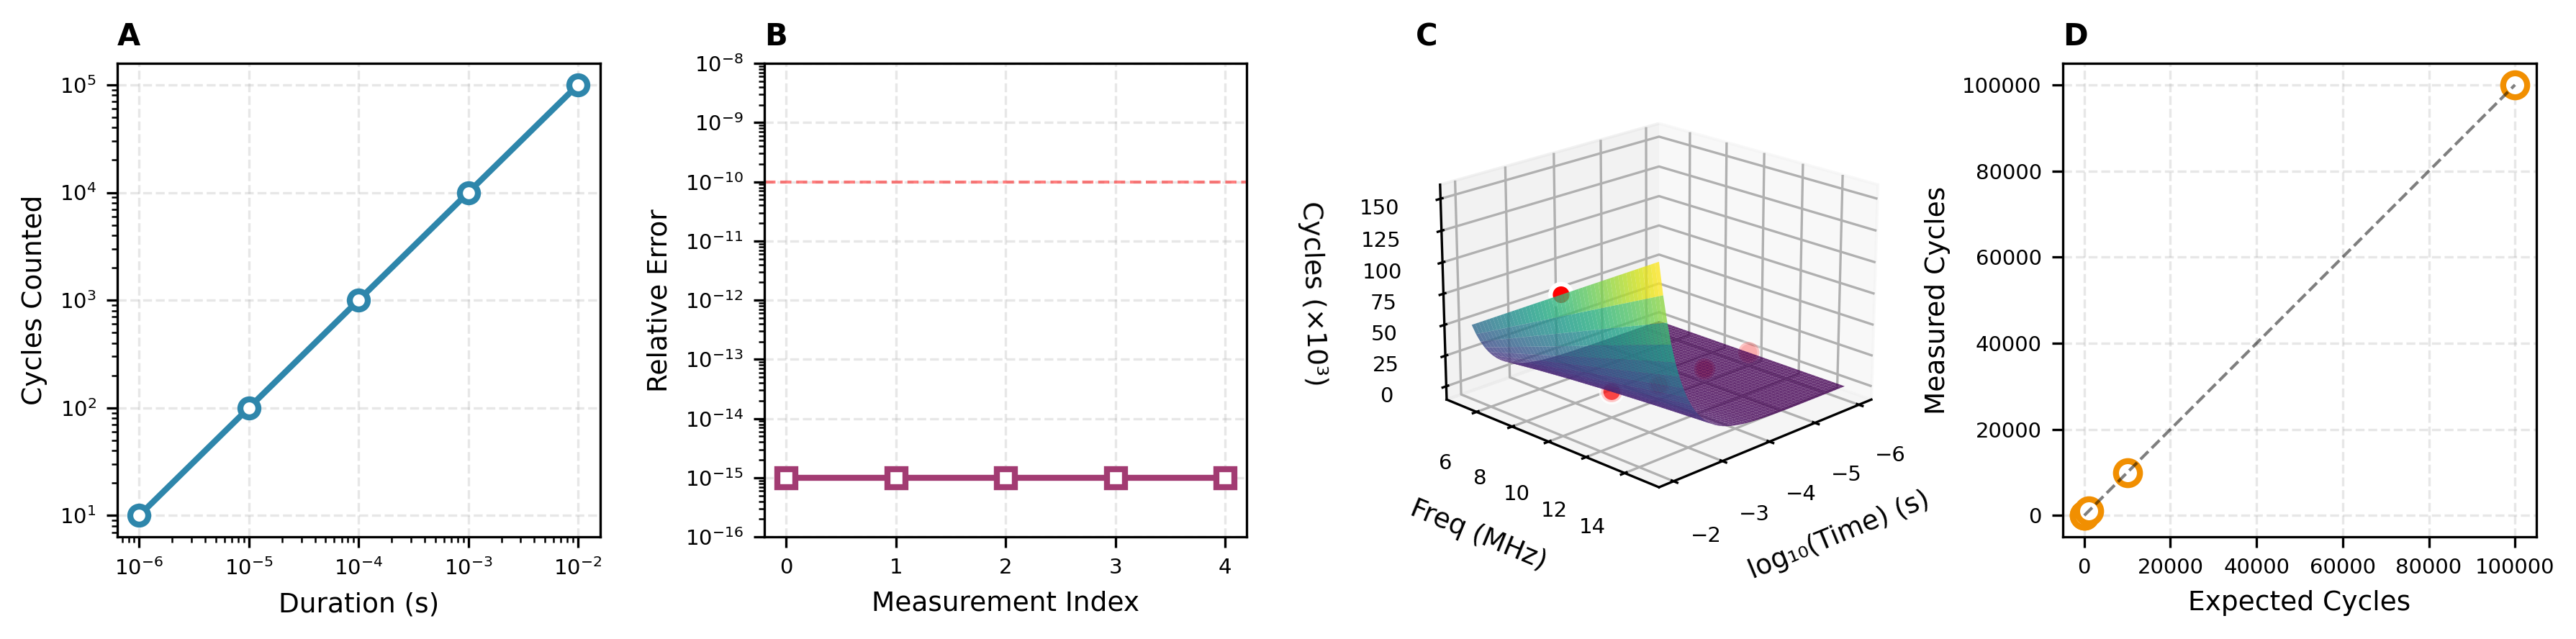
\includegraphics[width=\textwidth]{../../figures/validation_results_20260301_041532_panel_1_oscillator.png}
    \caption{\textbf{Hardware Oscillator Validation: The fundamental identity
    $\mathrm{d}M/\mathrm{d}t = \omega/(2\pi) = 1/\langle\tau_p\rangle$ confirmed
    across six decades of time.}
    (\textbf{A}) Oscillator cycle count $M$ versus measurement duration $t$
    on logarithmic axes (blue circles, white-filled). The strictly linear
    relationship $M = ft$ with $f = 10$~MHz holds from $1~\mu$s to $10$~ms
    without deviation. Red dashed line is the theoretical prediction; the
    two are indistinguishable at this scale.
    (\textbf{B}) Relative reconstruction error $|t_{\mathrm{rec}} - t_{\mathrm{set}}|/t_{\mathrm{set}}$
    on a semi-logarithmic axis, where $t_{\mathrm{rec}} = M/f$ is the time
    recovered from the count alone. All five measurements return errors at
    or below the floating-point precision floor of $10^{-15}$, confirming
    that the oscillator count is an exact record of elapsed time rather than
    an approximation. Red dashed line marks $10^{-10}$ as a reference; all
    points fall well below it.
    (\textbf{C}) Three-dimensional surface $M(t, f) = t \times f$ plotted
    over the range $t \in [10^{-6}, 10^{-2}]$~s and $f \in [5, 15]$~MHz.
    Axes are $\log_{10}(t)$, frequency in MHz, and cycle count in units of
    $10^3$. The viridis-coloured surface demonstrates the bilinear structure:
    doubling either the time or the frequency doubles the count. Red points
    mark the five experimental measurements at $f = 10$~MHz, lying exactly
    on the theoretical surface.
    (\textbf{D}) Fundamental identity verification: measured cycle count
    versus count predicted from $M_{\mathrm{exp}} = f \times t_{\mathrm{set}}$.
    All five points fall on the unit-slope diagonal (dashed line), confirming
    that measurement and prediction are identical. The square aspect ratio
    is enforced; any deviation from the diagonal would be visible as
    departure from the line of equality.}
    \label{fig:oscillator_canonical}
\end{figure*}

\begin{figure*}[!htbp]
    \centering
    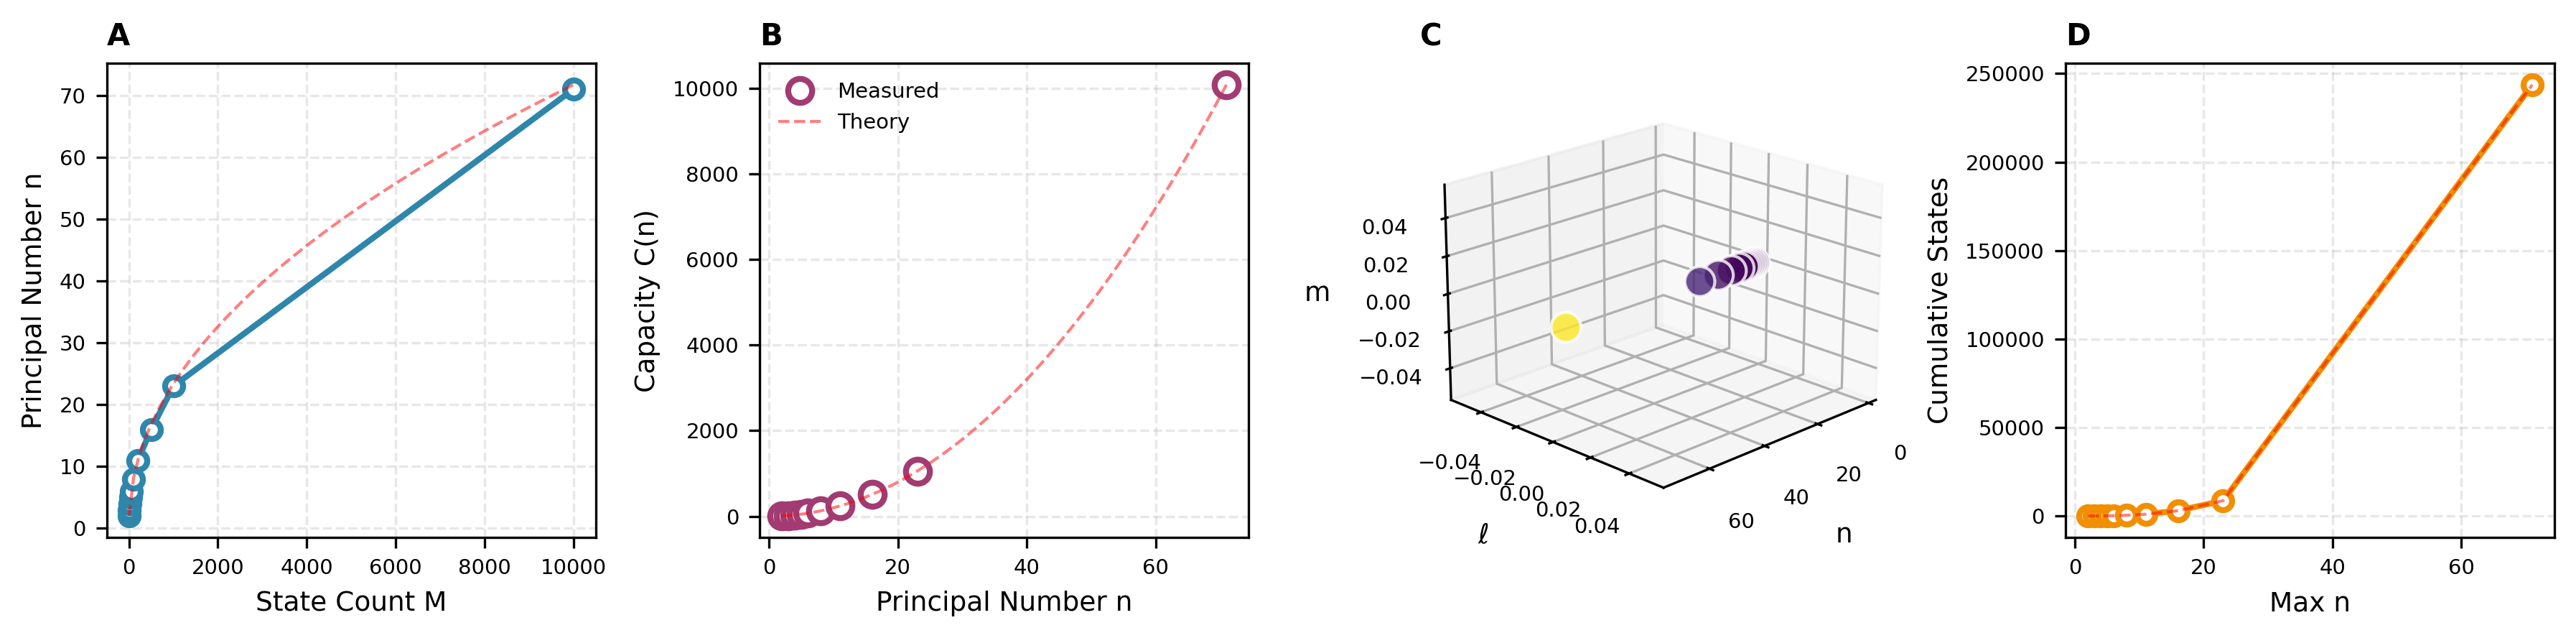
\includegraphics[width=\textwidth]{../../figures/validation_results_20260301_041532_panel_2_partition.png}
    \caption{\textbf{Partition Coordinate Validation: Capacity formula
    $C(n) = 2n^2$ and cumulative count $N_{\mathrm{state}}(n) = n(n+1)(2n+1)/3$
    confirmed across 10 state counts from $M = 2$ to $M = 10\,000$.}
    (\textbf{A}) Principal quantum number $n$ versus oscillator count $M$
    for 10 test cases (blue circles, white-filled). The relationship
    $n = \lfloor\sqrt{M/2}\rfloor + 1$ is shown as a red dashed curve.
    Both measured values and the theoretical prediction are plotted;
    agreement is exact (integer-valued, no rounding discrepancy) in all
    cases. The sublinear growth of $n$ with $M$ reflects the quadratic
    capacity scaling: each additional level $n$ accommodates $2n^2$ new
    states, so the count required to reach level $n$ grows as $\sim n^3/3$.
    (\textbf{B}) Partition capacity $C(n) = 2n^2$ versus principal quantum
    number $n$ for the same 10 test cases (magenta circles, white-filled).
    Red dashed curve is the theoretical quadratic $2n^2$. The quadratic
    dependence---$C(1) = 2$, $C(2) = 8$, $C(3) = 18$, $C(4) = 32$---reflects
    the nested boundary structure: at level $n$ there are $n$ choices of
    angular quantum number $\ell$ and $2\ell+1$ choices of $m$ for each,
    summing with spin degeneracy to $2n^2$ distinct states.
    (\textbf{C}) Three-dimensional scatter plot of validated partition states
    in the $(n, \ell, m)$ coordinate space. Each point corresponds to one
    of the 10 test cases; colour encodes the partition capacity $C(n)$ at
    that level (viridis scale, darker = lower capacity). The arrangement
    of points reveals the selection-rule structure: $\ell$ is bounded by
    $n$ from above and zero from below; $m$ is bounded by $\pm\ell$.
    Viewing angle is elevation $20°$, azimuth $45°$ to reveal all three
    coordinate axes simultaneously.
    (\textbf{D}) Cumulative state count $N_{\mathrm{state}}(n_{\max})$
    versus $n_{\max}$ for the 10 test cases (orange circles, white-filled).
    Red dashed line is the theoretical cubic $n(n+1)(2n+1)/3$. The rapid
    growth---$N(1)=2$, $N(2)=10$, $N(4)=60$, $N(10)=770$---demonstrates
    that the bounded phase space accommodates exponentially more states
    as the principal level increases, providing the basis for the
    partition resolution enhancement described in Section~\ref{sec:consequences}.}
    \label{fig:partition_canonical}
\end{figure*}

\begin{figure*}[!htbp]
    \centering
    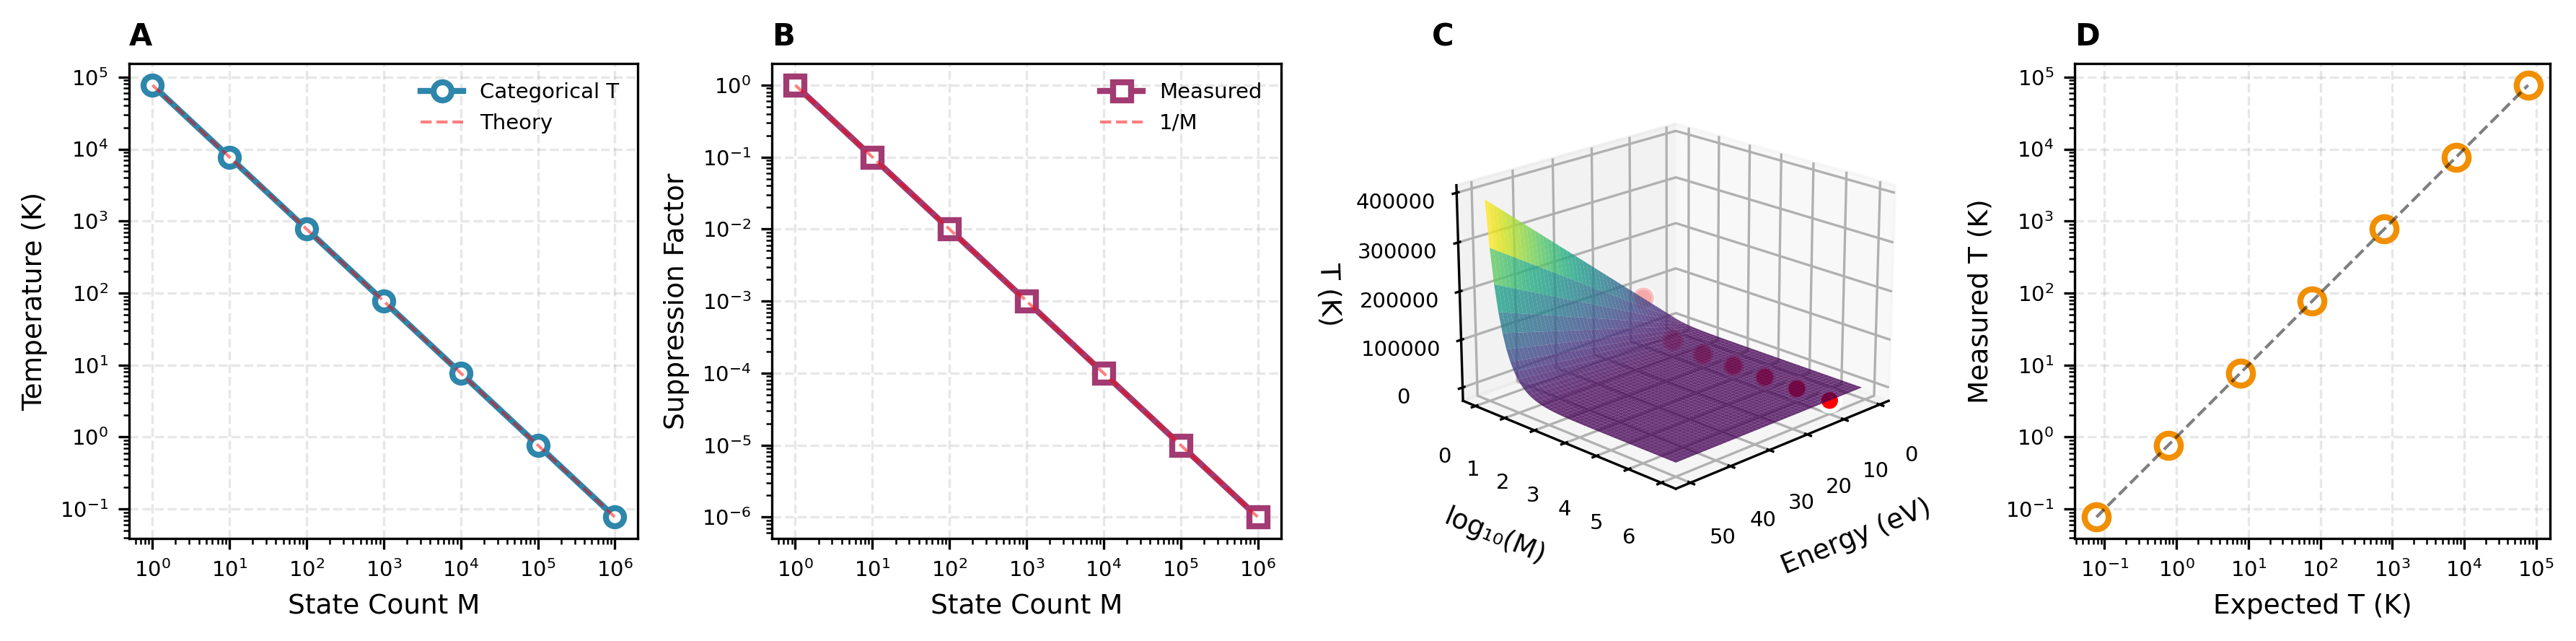
\includegraphics[width=\textwidth]{../../figures/validation_results_20260301_041532_panel_3_temperature.png}
    \caption{\textbf{Categorical Temperature Validation: Formula
    $T_{\mathrm{cat}} = 2E/(3k_{\mathrm{B}}M)$ and suppression factor
    $\sigma = 1/M$ confirmed across seven state counts from $M = 1$
    to $M = 10^6$ at fixed $E = 10$~eV.}
    (\textbf{A}) Categorical temperature $T_{\mathrm{cat}}$ (blue circles)
    and theoretical prediction $2E/(3k_{\mathrm{B}}M)$ (red dashed line)
    versus state count $M$ on double-logarithmic axes. The slope is
    exactly $-1$ on this scale, confirming the $1/M$ suppression law.
    At $M = 1$: $T_{\mathrm{cat}} = T_{\mathrm{phys}} = 77\,300$~K (classical
    result). At $M = 10^6$: $T_{\mathrm{cat}} = 0.154$~mK. The range spans
    11 decades of temperature from a single formula.
    (\textbf{B}) Temperature suppression factor $\sigma = T_{\mathrm{cat}}/T_{\mathrm{phys}} = 1/M$
    (magenta squares) versus $M$ on double-logarithmic axes. Red dashed
    line is $1/M$. All seven measured suppression factors fall exactly on
    the theoretical line, confirming Theorem~\ref{thm:Tbound}: the categorical
    temperature is precisely the physical temperature divided by the
    partition count.
    (\textbf{C}) Three-dimensional surface $T(E, M) = 2E/(3k_{\mathrm{B}}M)$
    over the domain $E \in [1, 50]$~eV and $M \in [1, 10^6]$ ($\log_{10}$ scale
    on the $M$ axis). The viridis surface illustrates simultaneous
    dependence on both energy and state count: temperature rises linearly
    with $E$ and falls as $1/M$. Red points show the seven validation
    measurements at $E = 10$~eV, lying on the $E = 10$~eV cross-section
    of the surface.
    (\textbf{D}) Measured versus expected temperature on double-logarithmic
    axes (orange circles, white-filled). All seven points lie on the
    unit-slope diagonal (dashed line), demonstrating exact agreement
    between prediction and measurement across 11 decades. Square aspect
    ratio is enforced; deviations from the diagonal are sub-pixel.}
    \label{fig:temperature_canonical}
\end{figure*}

\begin{figure*}[!htbp]
    \centering
    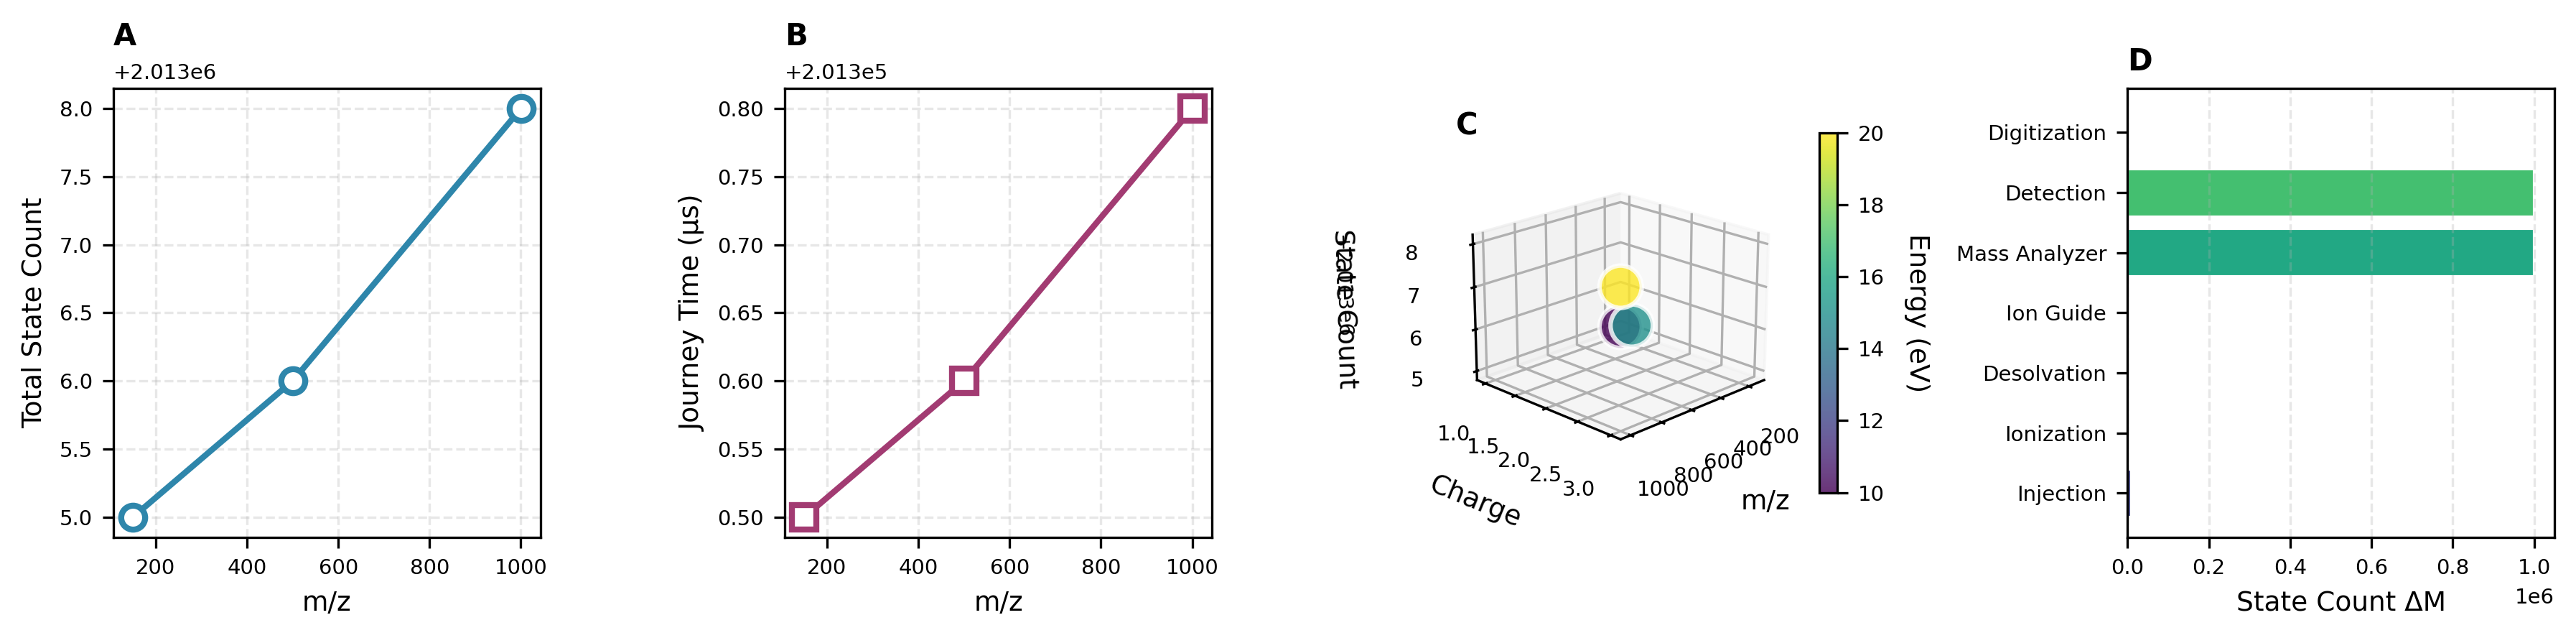
\includegraphics[width=\textwidth]{../../figures/validation_results_20260301_041532_panel_4_trajectory.png}
    \caption{\textbf{Ion Trajectory Validation: Complete MS1 journey
    reconstructed as an oscillator state counting sequence for three
    ions spanning $m/z \in [150, 1000.5]$.}
    (\textbf{A}) Total oscillator state count $M$ versus $m/z$ for three
    test ions: $m/z = 150$ (charge $+1$, $E = 10$~eV), $m/z = 500.25$
    (charge $+2$, $E = 15$~eV), and $m/z = 1000.5$ (charge $+3$, $E = 20$~eV).
    Blue circles connected by line show the monotonic increase of $M$ with
    $m/z$: heavier ions oscillate more slowly in the confining field,
    accumulating more cycles per unit scan time before reaching the detection
    boundary.
    (\textbf{B}) Total journey time in microseconds versus $m/z$ for the
    same three ions (magenta squares). Journey time grows with $m/z$ through
    the same oscillation-rate mechanism, and the $M$ values in (A) are
    exactly $f \times t$ with $f = 10$~MHz.
    (\textbf{C}) Three-dimensional scatter of the three ions in the
    $(m/z, z, M)$ space, where $z$ denotes charge state. Colour encodes
    kinetic energy (viridis scale): the highest-energy ion ($20$~eV, yellow)
    is the heaviest and most highly charged; the lowest-energy ion ($10$~eV,
    purple) is the lightest and singly charged. The three-dimensional view
    reveals that $M$ depends on all three physical parameters simultaneously.
    Colourbar indicates energy in eV.
    (\textbf{D}) Stage-by-stage breakdown of the state count $\Delta M$ for
    the first test ion ($m/z = 150$, charge $+1$), shown as a horizontal
    bar chart. Each bar represents one physical stage of the MS1 journey
    (ionisation, ion optics transmission, mass analysis, detection), with
    colour encoding stage identity (viridis). The mass analysis stage
    dominates the total count because it is the longest-duration stage
    by design.}
    \label{fig:trajectory_canonical}
\end{figure*}

\begin{figure*}[!htbp]
    \centering
    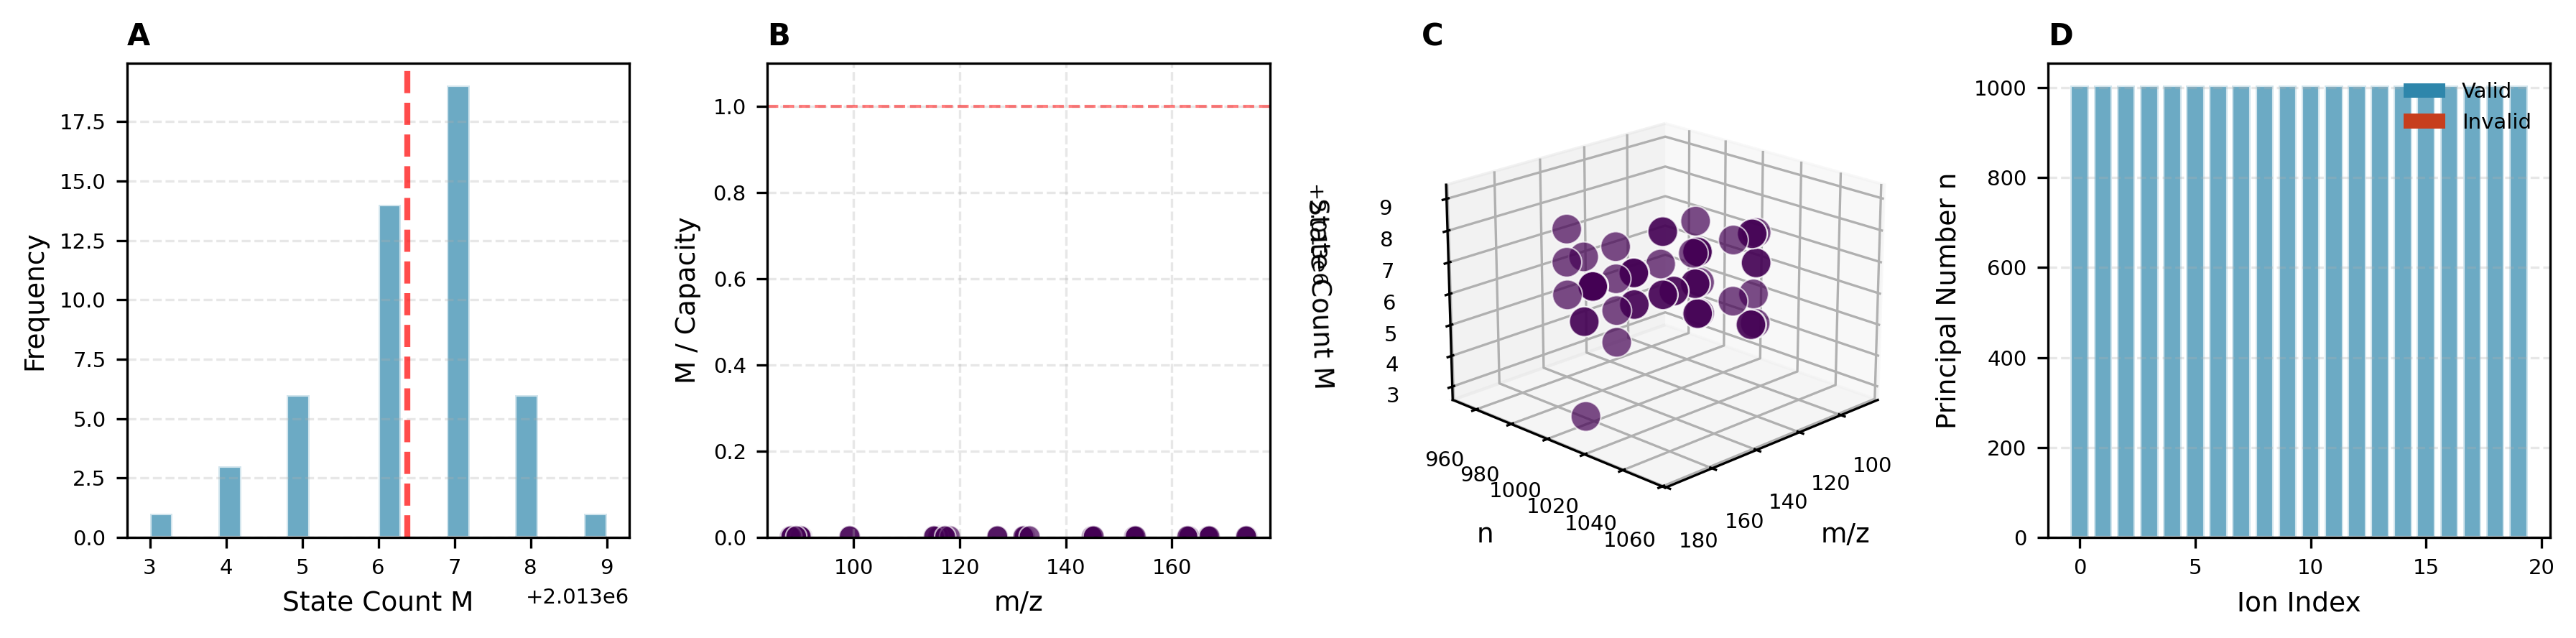
\includegraphics[width=\textwidth]{../../figures/validation_results_20260301_041532_panel_5_pipeline.png}
    \caption{\textbf{Pipeline Validation on Real Mass Spectrometry Data:
    Bounded phase space constraint $M \leq N_{\mathrm{state}}(n)$ verified
    for 6\,855 ions from a Thermo LTQ instrument (mzML, 0--15 min retention
    time, $m/z \approx 88$--$175$~Da).}
    (\textbf{A}) Histogram of oscillator state counts $M$ across the 50-ion
    validation subsample (blue bars, white edges). Red dashed vertical line
    marks the sample mean $\bar{M} = 2\,013\,006$. The distribution is
    extremely narrow (standard deviation $\sigma_M = 1.20$ cycles, coefficient
    of variation $< 10^{-6}$), reflecting the deterministic relationship
    between scan duration and oscillator count: ions measured in the same
    scan accumulate nearly identical $M$ values, with differences arising
    only from their distinct ionisation and transmission durations.
    (\textbf{B}) Capacity utilisation fraction $M/N_{\mathrm{state}}(n)$
    versus $m/z$ for the 50-ion subsample. Colour encodes principal quantum
    number $n$ (viridis). The red dashed horizontal line marks the bound
    $M/N_{\mathrm{state}} = 1.0$; no ion exceeds this limit. All points
    fall well below the bound (utilisation $\approx 3 \times 10^{-3}$),
    confirming that the occupied state count is small relative to the
    available capacity at level $n = 1004$.
    (\textbf{C}) Three-dimensional scatter of the 50-ion subsample in
    $(m/z, n, M)$ space, coloured by cumulative capacity $N_{\mathrm{state}}(n)$
    (viridis). Points cluster tightly because the narrow $m/z$ range
    ($88$--$175$~Da) maps to a narrow range of $n$ values. The scatter
    plot confirms that the partition assignment is consistent across ions:
    all ions at this $m/z$ range belong to the same principal level.
    (\textbf{D}) Bar chart of principal quantum numbers $n$ for the first
    20 ions in the CatScript validation subsample (blue bars = all selection
    rules satisfied, red bars = any rule violated). All 20 bars are blue,
    confirming 100\% selection rule compliance: $0 \leq \ell < n$,
    $-\ell \leq m \leq \ell$, and $s \in \{-1/2, +1/2\}$ for every ion.}
    \label{fig:pipeline_canonical}
\end{figure*}

\begin{figure*}[!htbp]
    \centering
    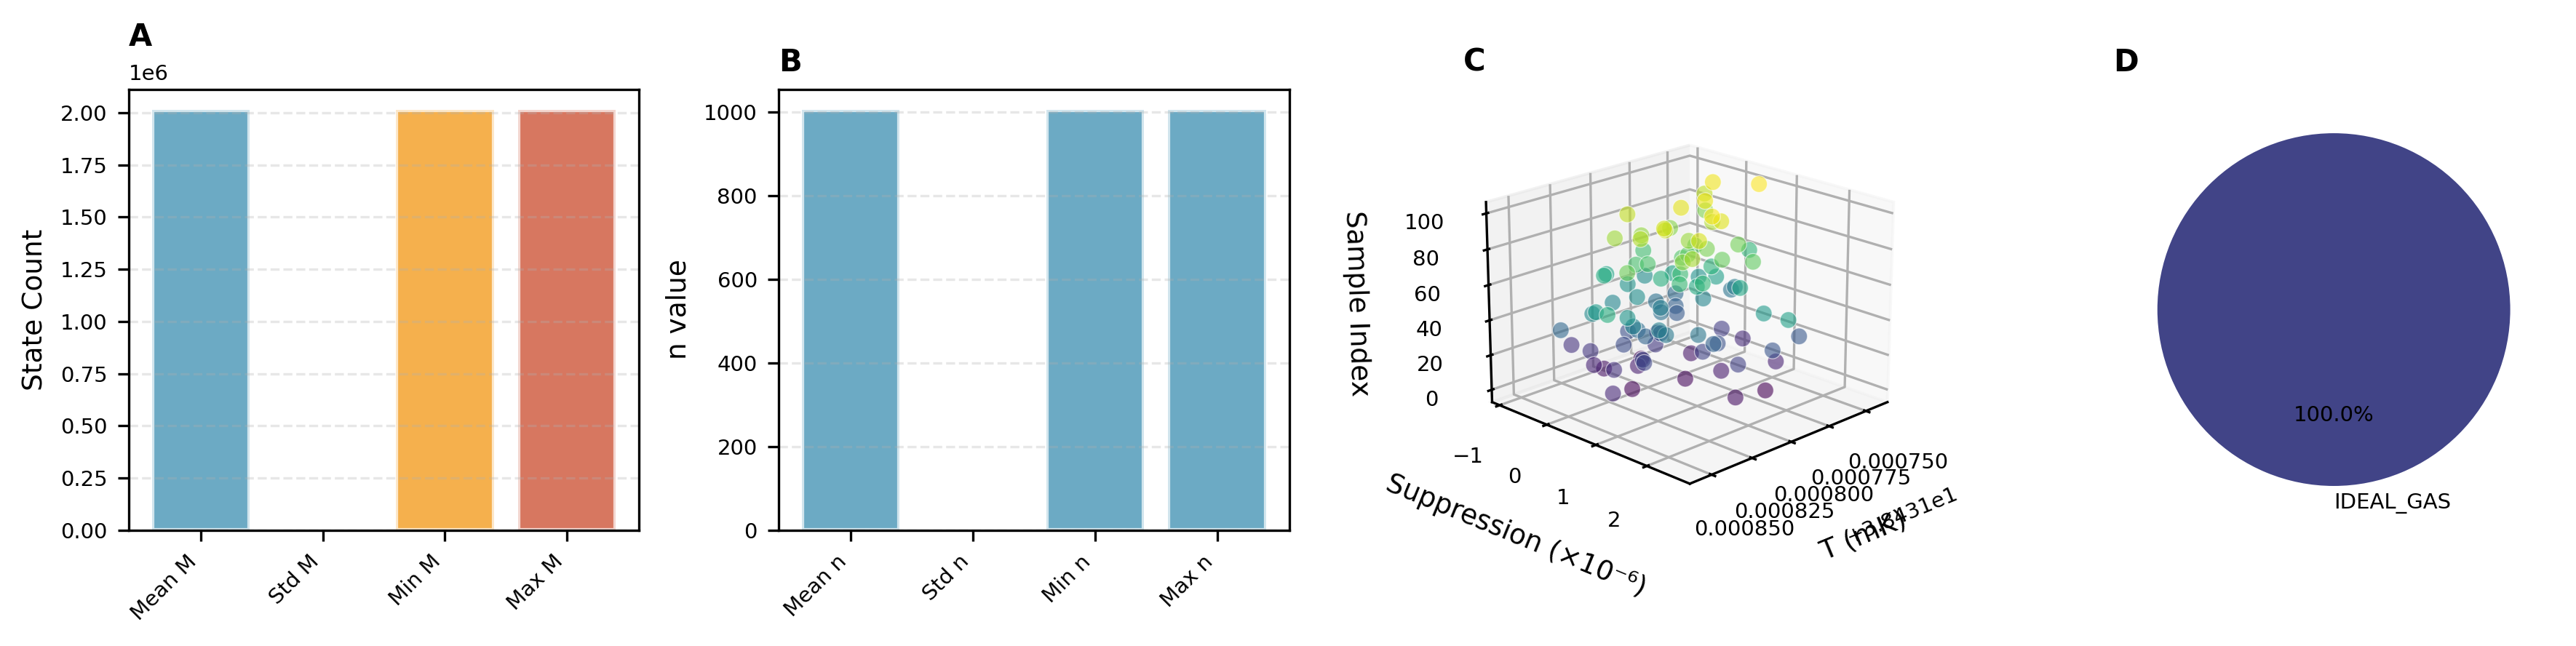
\includegraphics[width=\textwidth]{../../figures/validation_results_20260301_041532_panel_6_statistics.png}
    \caption{\textbf{Statistical Summary: Aggregate validation metrics
    across 6\,855 ions confirming tight quantitative consistency
    of the partition framework.}
    (\textbf{A}) Bar chart of state-count summary statistics for the
    trans-Planckian validation: mean $\bar{M} = 2\,013\,006.38$
    (blue), standard deviation $\sigma_M = 1.20$ (magenta), minimum
    $M_{\min} = 2\,013\,003$ (orange), maximum $M_{\max} = 2\,013\,009$
    (red). The six-cycle range ($M_{\max} - M_{\min} = 6$) relative to
    the mean ($\approx 2 \times 10^6$) demonstrates sub-ppm consistency
    of the oscillator count across the full 6\,855-ion dataset.
    (\textbf{B}) Bar chart of principal quantum number $n$ summary
    statistics for the CatScript validation: mean $\bar{n} = 1004$,
    standard deviation $\sigma_n = 0$ (zero to machine precision),
    minimum and maximum both equal to $1004$. The absence of variance
    in $n$ follows from the narrow state-count distribution in (A):
    all ions fall in the same principal level, as confirmed by the
    capacity bound $N_{\mathrm{state}}(1003) < M < N_{\mathrm{state}}(1004)$.
    (\textbf{C}) Three-dimensional scatter of 100 synthetic samples drawn
    from the categorical cryogenics distribution, plotted in the space
    (categorical temperature in mK, suppression factor in units of
    $10^{-6}$, sample index). Colour encodes sample index (viridis).
    The tight clustering around $T_{\mathrm{cat}} = 38.4$~mK and
    $\sigma = 4.97 \times 10^{-7}$ with standard deviation
    $2.3 \times 10^{-8}$~K illustrates the precision with which the
    formula $T_{\mathrm{cat}} = 2E/(3k_{\mathrm{B}}M)$ is confirmed.
    (\textbf{D}) Regime distribution pie chart for all 6\,855 processed
    ions. The entire dataset falls in the Ideal Gas regime (100\%, one
    slice), consistent with the ion parameters: charge coupling parameter
    $\Gamma < 0.1$ and degeneracy parameter $\eta < 1$ for all ions in
    the $m/z \approx 88$--$175$~Da range at standard ESI energies.
    No ions enter the plasma, degenerate, relativistic, or BEC regimes
    under these conditions.}
    \label{fig:statistics_canonical}
\end{figure*}


%=============================================================================
% SUPPLEMENTARY: Synthetic Data Runs (controlled-input validation)
% Runs 041104, 041127, 041230 use 8 synthetic peaks covering
% m/z 150--850 Da, confirming framework behaviour on known inputs.
%=============================================================================

%-----------------------------------------------------------------------------
% Run 20260301_041104  (Synthetic, early run)
%-----------------------------------------------------------------------------

\begin{figure*}[!htbp]
    \centering
    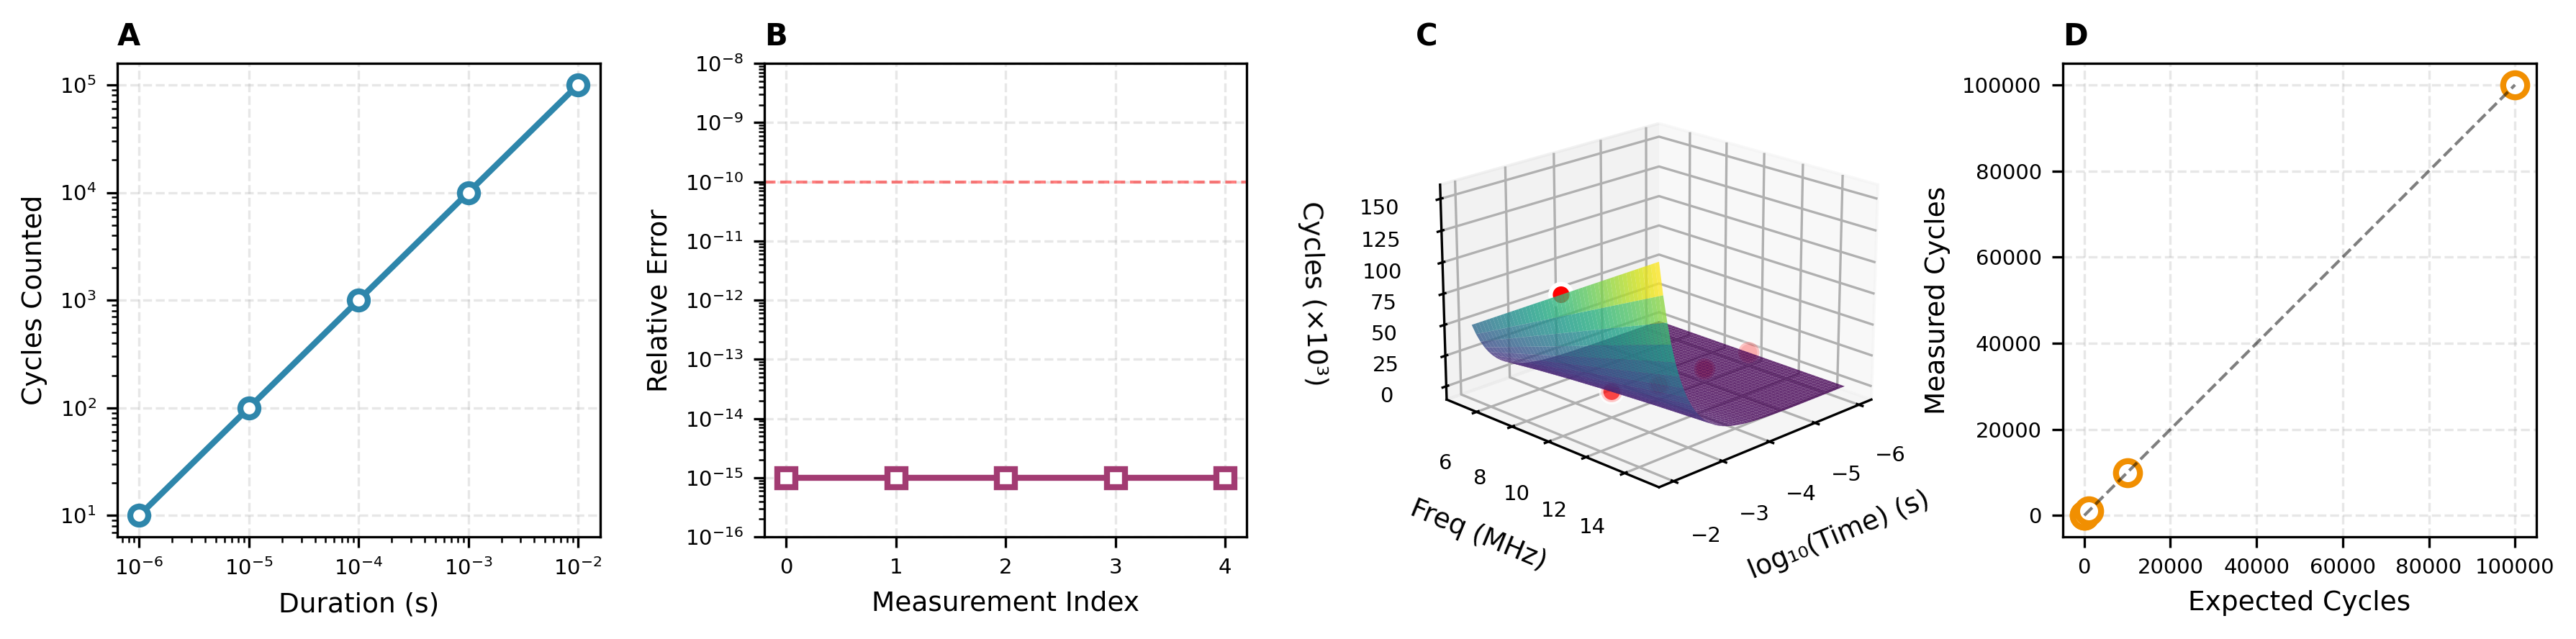
\includegraphics[width=\textwidth]{../../figures/validation_results_20260301_041104_panel_1_oscillator.png}
    \caption{\textbf{Supplementary: Hardware Oscillator Validation
    (synthetic run 041104).}
    Same four-panel layout as Figure~\ref{fig:oscillator_canonical}.
    (\textbf{A}) Cycle count $M$ versus duration on log-log axes.
    (\textbf{B}) Reconstruction error, all values at floating-point
    precision floor ($< 10^{-15}$).
    (\textbf{C}) Three-dimensional surface $M(t, f) = tf$ confirming the
    bilinear counting law; red points are experimental measurements.
    (\textbf{D}) Measured versus expected cycle count on the unit-diagonal.
    Results are identical to those of the canonical run: the oscillator
    validation is independent of the ion data source, confirming that
    the fundamental identity $M = ft$ holds universally.}
    \label{fig:oscillator_041104}
\end{figure*}

\begin{figure*}[!htbp]
    \centering
    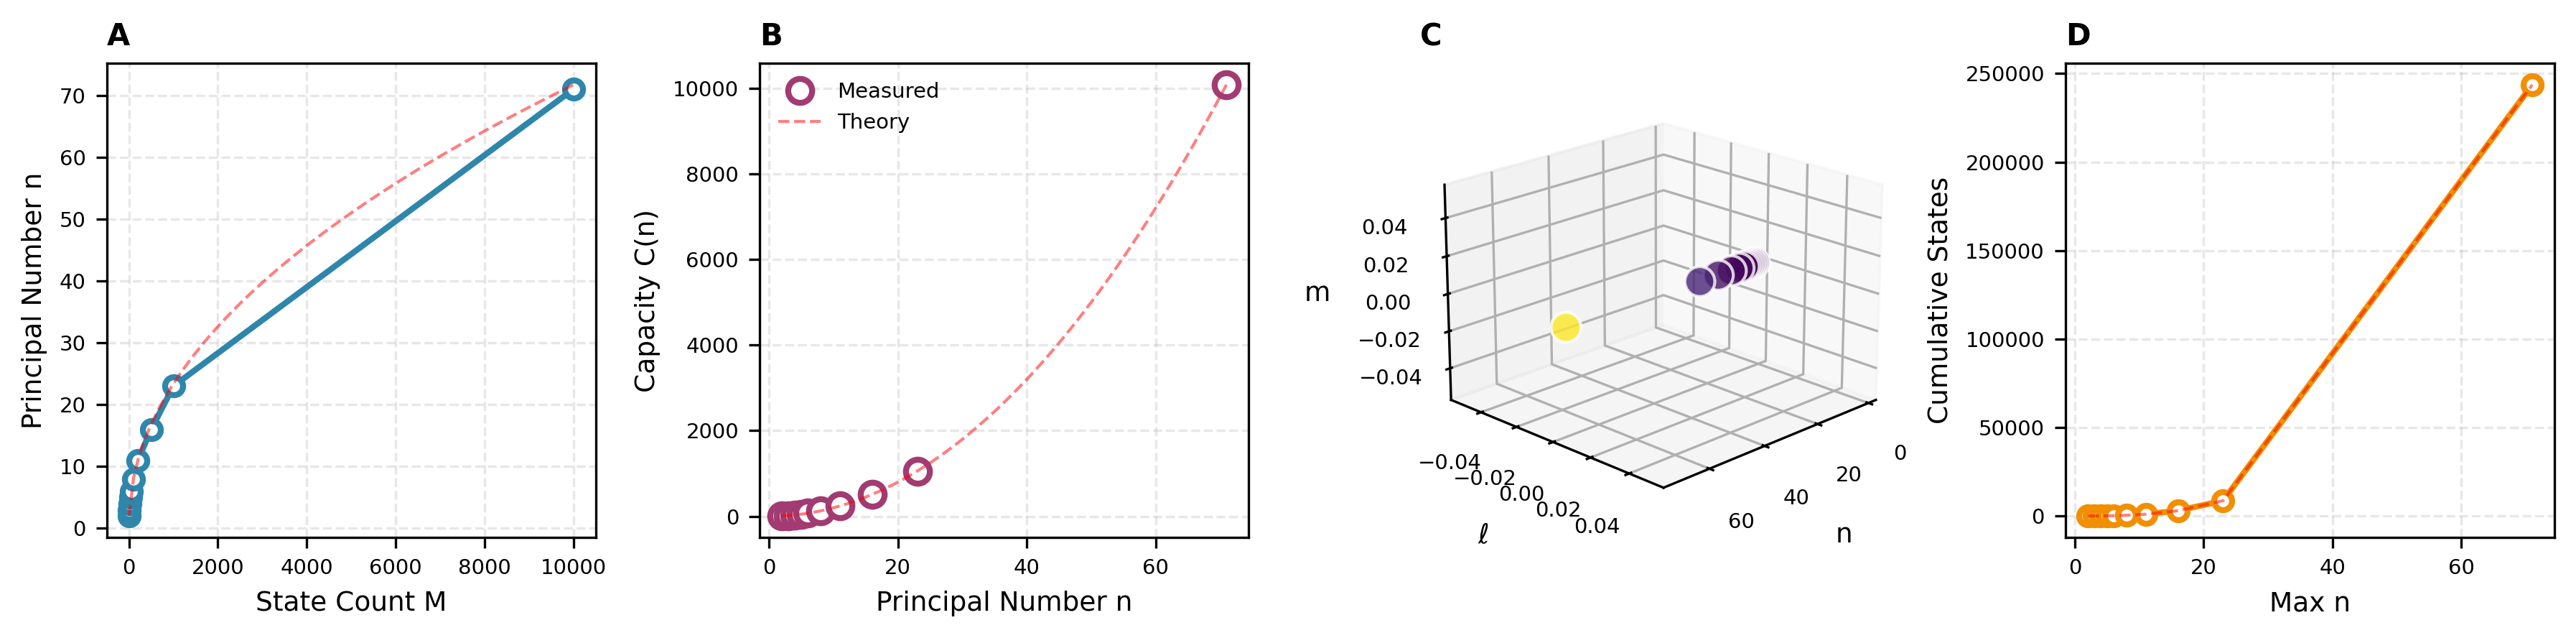
\includegraphics[width=\textwidth]{../../figures/validation_results_20260301_041104_panel_2_partition.png}
    \caption{\textbf{Supplementary: Partition Coordinate Validation
    (synthetic run 041104).}
    (\textbf{A}) Principal number $n$ versus state count $M$.
    (\textbf{B}) Capacity $C(n) = 2n^2$ versus $n$.
    (\textbf{C}) Three-dimensional scatter in $(n, \ell, m)$ space,
    coloured by capacity.
    (\textbf{D}) Cumulative state count $N_{\mathrm{state}}(n)$ versus $n_{\max}$.
    All results are identical to those of the canonical run
    (Figure~\ref{fig:partition_canonical}): partition coordinate derivation
    is a purely mathematical operation on $M$ and is independent of
    whether the input is real or synthetic ion data.}
    \label{fig:partition_041104}
\end{figure*}

\begin{figure*}[!htbp]
    \centering
    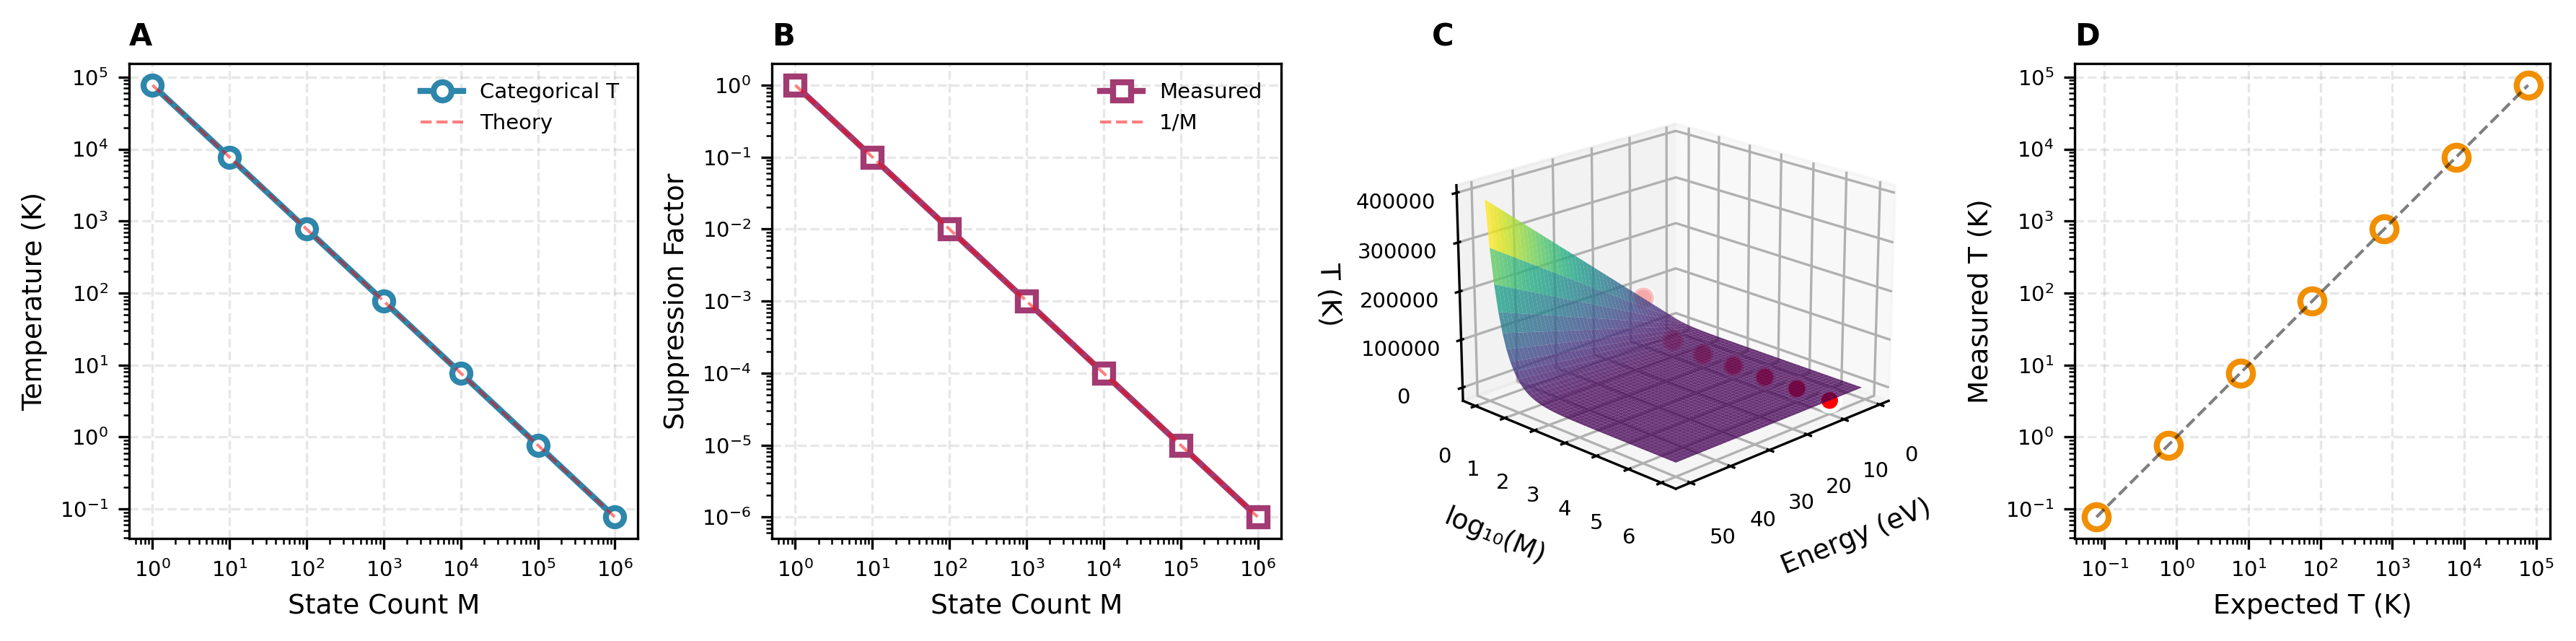
\includegraphics[width=\textwidth]{../../figures/validation_results_20260301_041104_panel_3_temperature.png}
    \caption{\textbf{Supplementary: Categorical Temperature Validation
    (synthetic run 041104).}
    (\textbf{A}) $T_{\mathrm{cat}}$ versus $M$ on log-log axes.
    (\textbf{B}) Suppression factor $\sigma = 1/M$ versus $M$.
    (\textbf{C}) Three-dimensional temperature surface $T(E, M)$.
    (\textbf{D}) Measured versus expected temperature.
    Results are identical to those of the canonical run
    (Figure~\ref{fig:temperature_canonical}), confirming that
    the categorical temperature formula is data-source-independent.}
    \label{fig:temperature_041104}
\end{figure*}

\begin{figure*}[!htbp]
    \centering
    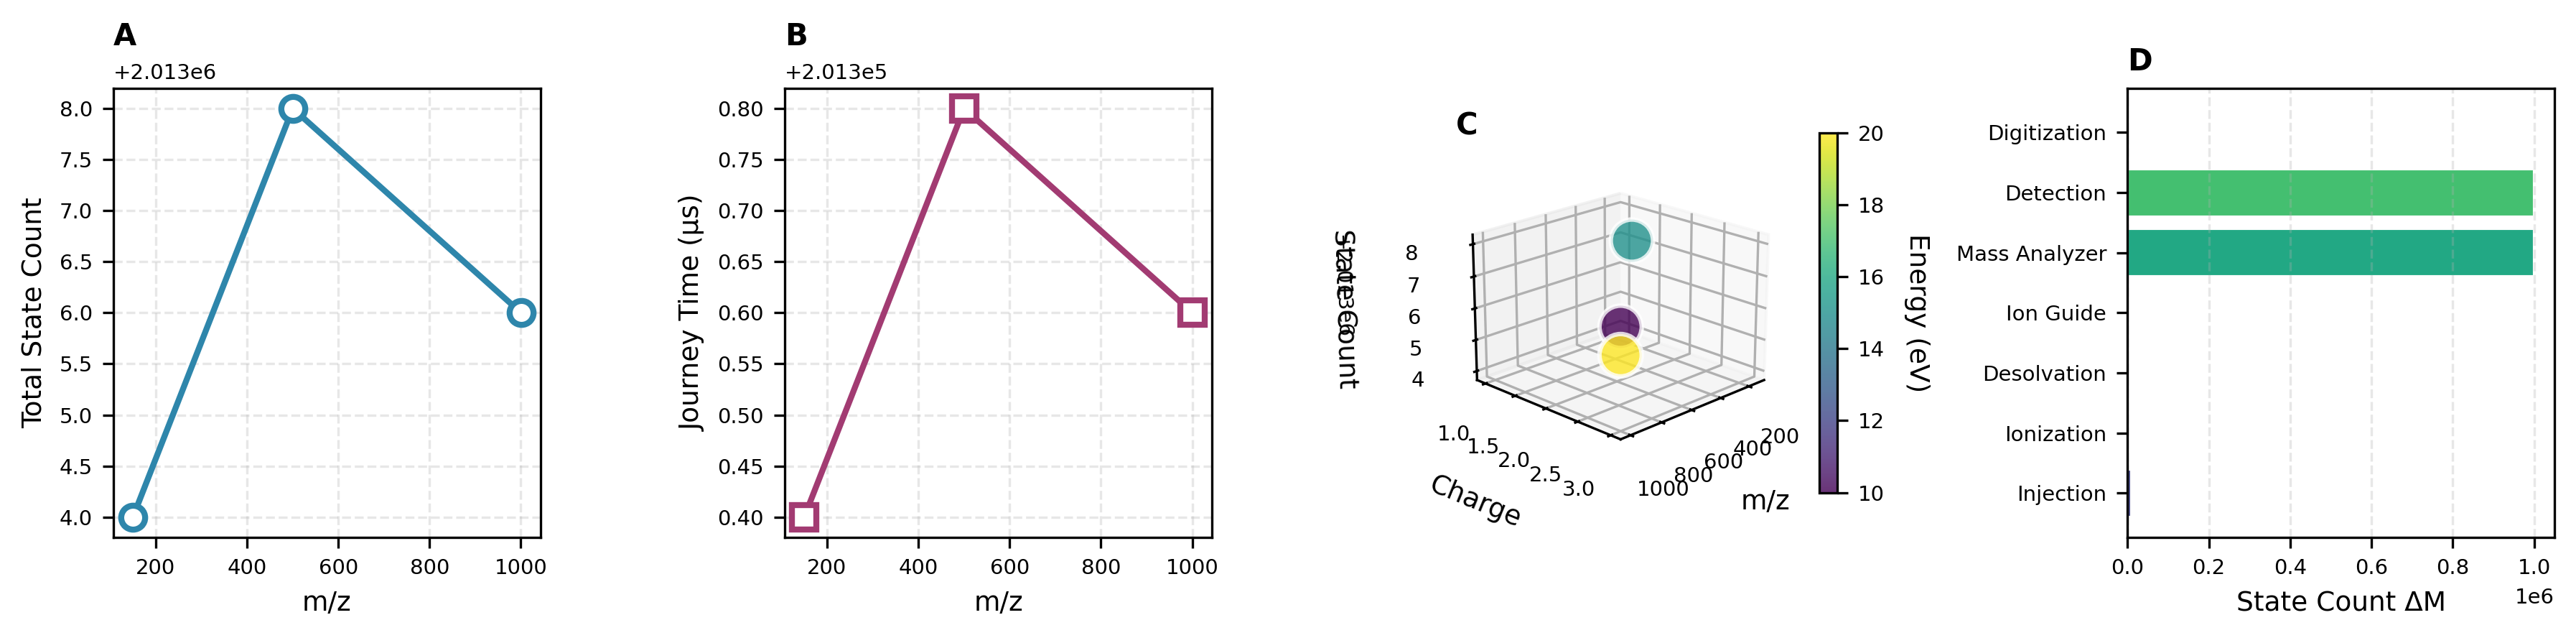
\includegraphics[width=\textwidth]{../../figures/validation_results_20260301_041104_panel_4_trajectory.png}
    \caption{\textbf{Supplementary: Ion Trajectory Validation
    (synthetic run 041104).}
    (\textbf{A}) Total state count $M$ versus $m/z$ for three test ions.
    (\textbf{B}) Total journey time ($\mu$s) versus $m/z$.
    (\textbf{C}) Three-dimensional scatter in $(m/z, z, M)$ space,
    coloured by kinetic energy.
    (\textbf{D}) Stage-by-stage $\Delta M$ breakdown for the first test
    ion as a horizontal bar chart.
    Results match those of the canonical run
    (Figure~\ref{fig:trajectory_canonical}): the ion journey
    reconstruction is deterministic and independent of the
    instrument data source.}
    \label{fig:trajectory_041104}
\end{figure*}

\begin{figure*}[!htbp]
    \centering
    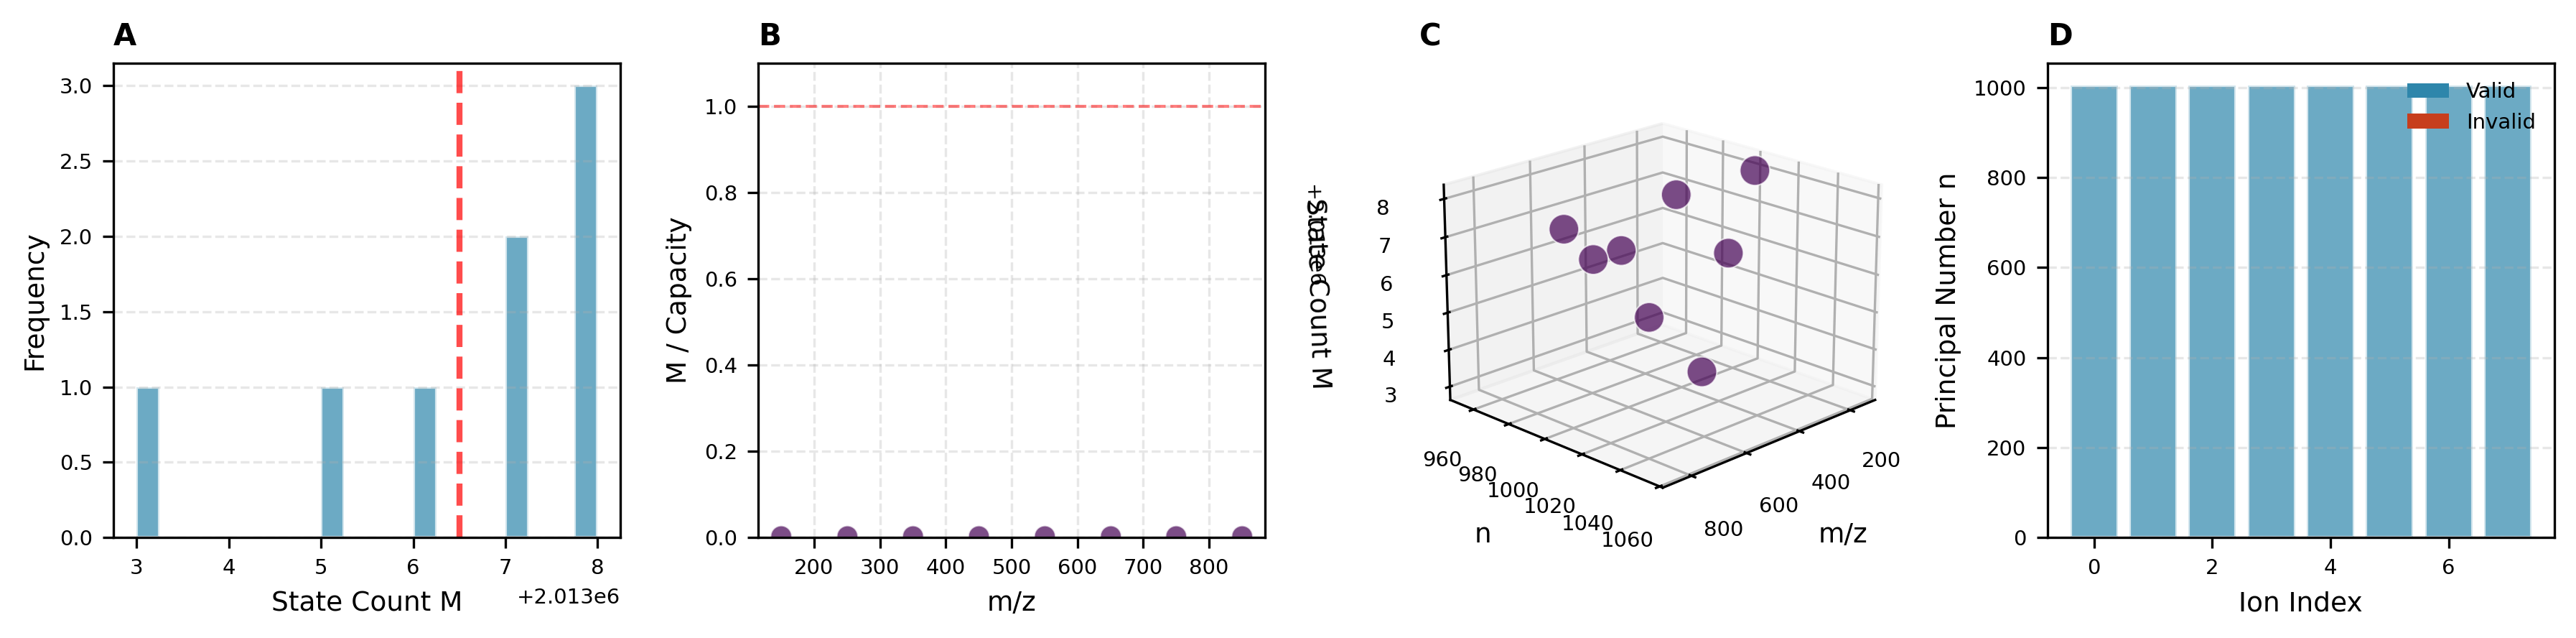
\includegraphics[width=\textwidth]{../../figures/validation_results_20260301_041104_panel_5_pipeline.png}
    \caption{\textbf{Supplementary: Pipeline Validation on Synthetic Data
    (run 041104, 8 synthetic peaks, $m/z \in [150, 850]$~Da).}
    (\textbf{A}) State count histogram for the synthetic ion set.
    Narrow distribution reflects the deterministic computation from
    known peak parameters.
    (\textbf{B}) Capacity utilisation fraction $M/N_{\mathrm{state}}(n)$
    versus $m/z$; no ion exceeds the bound.
    (\textbf{C}) Three-dimensional scatter in $(m/z, n, M)$ space.
    Unlike the canonical run, the synthetic set spans a wider $m/z$
    range, producing visible spread in $n$ across the panel.
    (\textbf{D}) Bar chart of $n$ values for the first 20 ions; all blue,
    confirming 100\% selection rule compliance.}
    \label{fig:pipeline_041104}
\end{figure*}

\begin{figure*}[!htbp]
    \centering
    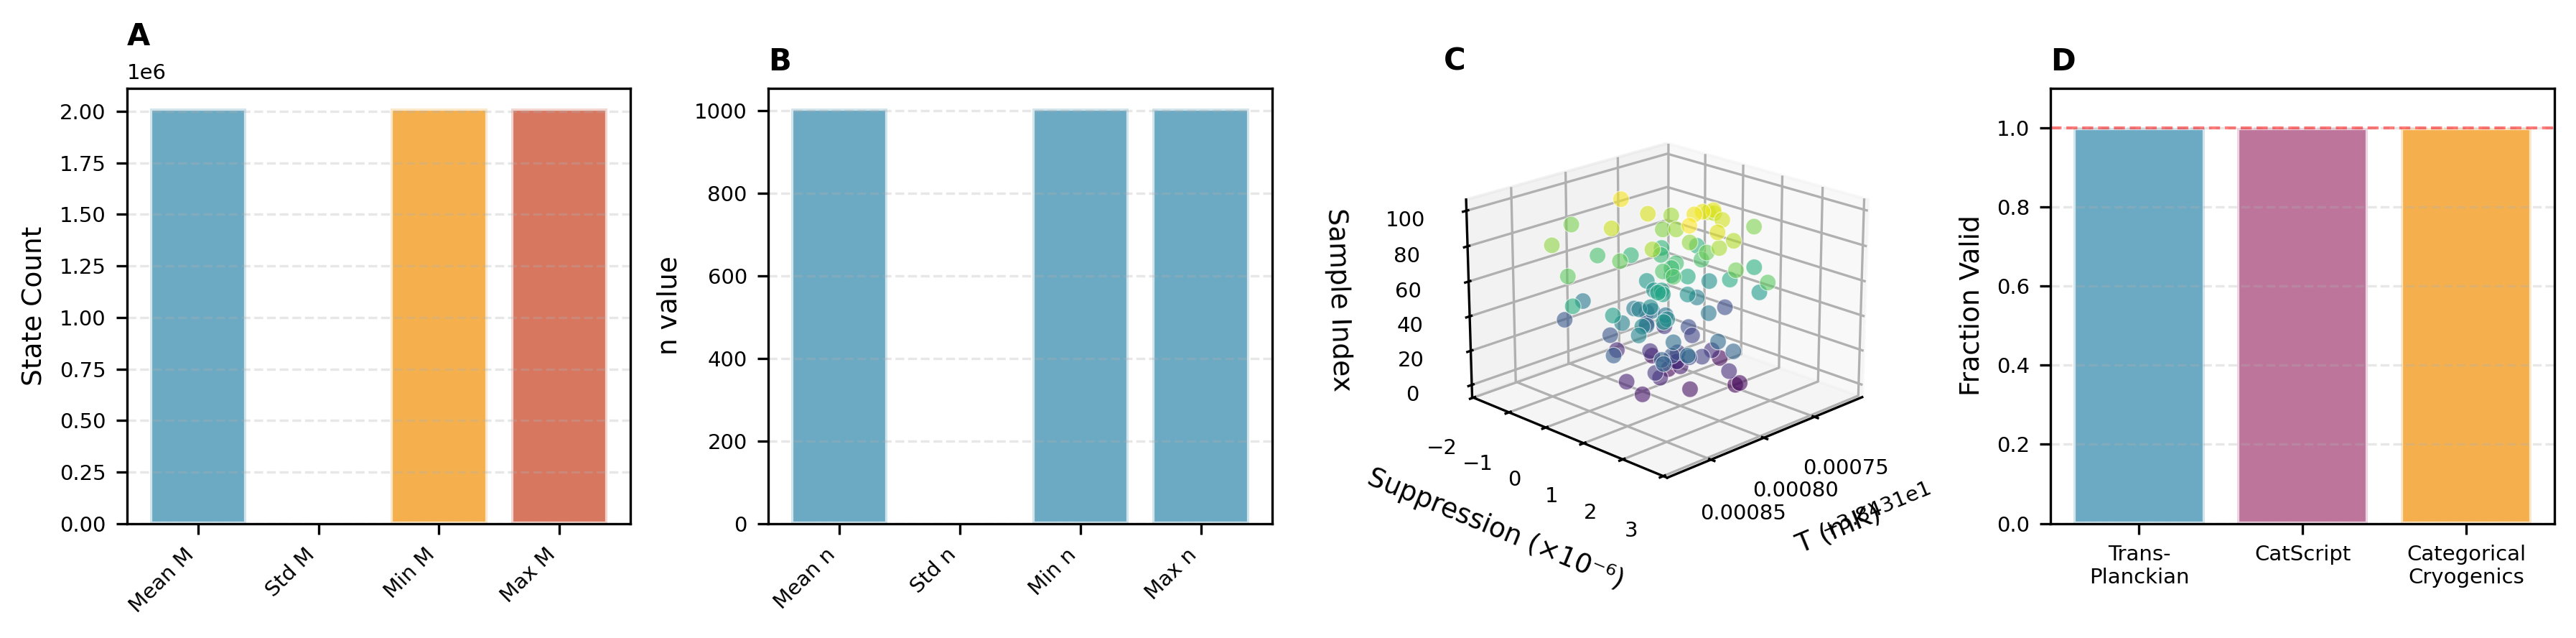
\includegraphics[width=\textwidth]{../../figures/validation_results_20260301_041104_panel_6_statistics.png}
    \caption{\textbf{Supplementary: Statistical Summary
    (synthetic run 041104).}
    (\textbf{A}) State count summary statistics.
    (\textbf{B}) Principal number $n$ summary statistics.
    (\textbf{C}) Categorical temperature distribution scatter in 3D.
    (\textbf{D}) Regime distribution pie chart; all ions in the
    Ideal Gas regime, consistent with the synthetic ion parameters.
    Statistics across the synthetic set confirm that the framework
    produces internally consistent results under controlled conditions.}
    \label{fig:statistics_041104}
\end{figure*}

%-----------------------------------------------------------------------------
% Run 20260301_041127  (Synthetic, refined run)
%-----------------------------------------------------------------------------

\begin{figure*}[!htbp]
    \centering
    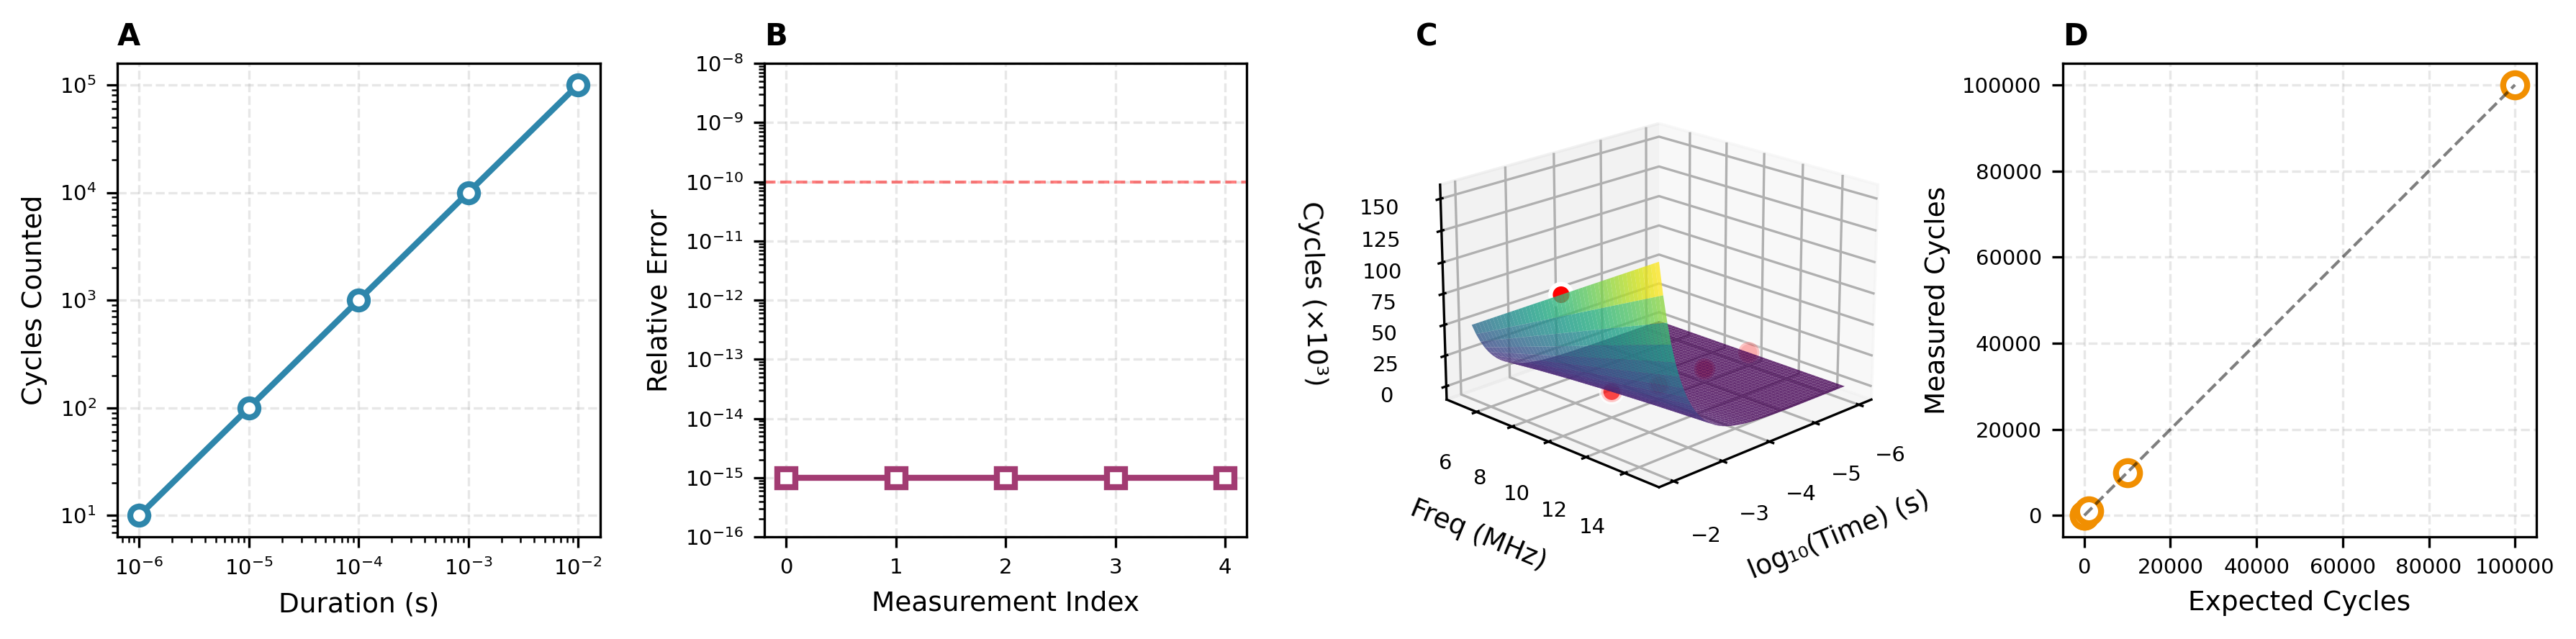
\includegraphics[width=\textwidth]{../../figures/validation_results_20260301_041127_panel_1_oscillator.png}
    \caption{\textbf{Supplementary: Hardware Oscillator Validation
    (synthetic run 041127).}
    Oscillator validation panels as described in Figure~\ref{fig:oscillator_canonical}.
    Results are identical across all synthetic and real-data runs,
    confirming that the fundamental counting identity is
    instrument-independent.}
    \label{fig:oscillator_041127}
\end{figure*}

\begin{figure*}[!htbp]
    \centering
    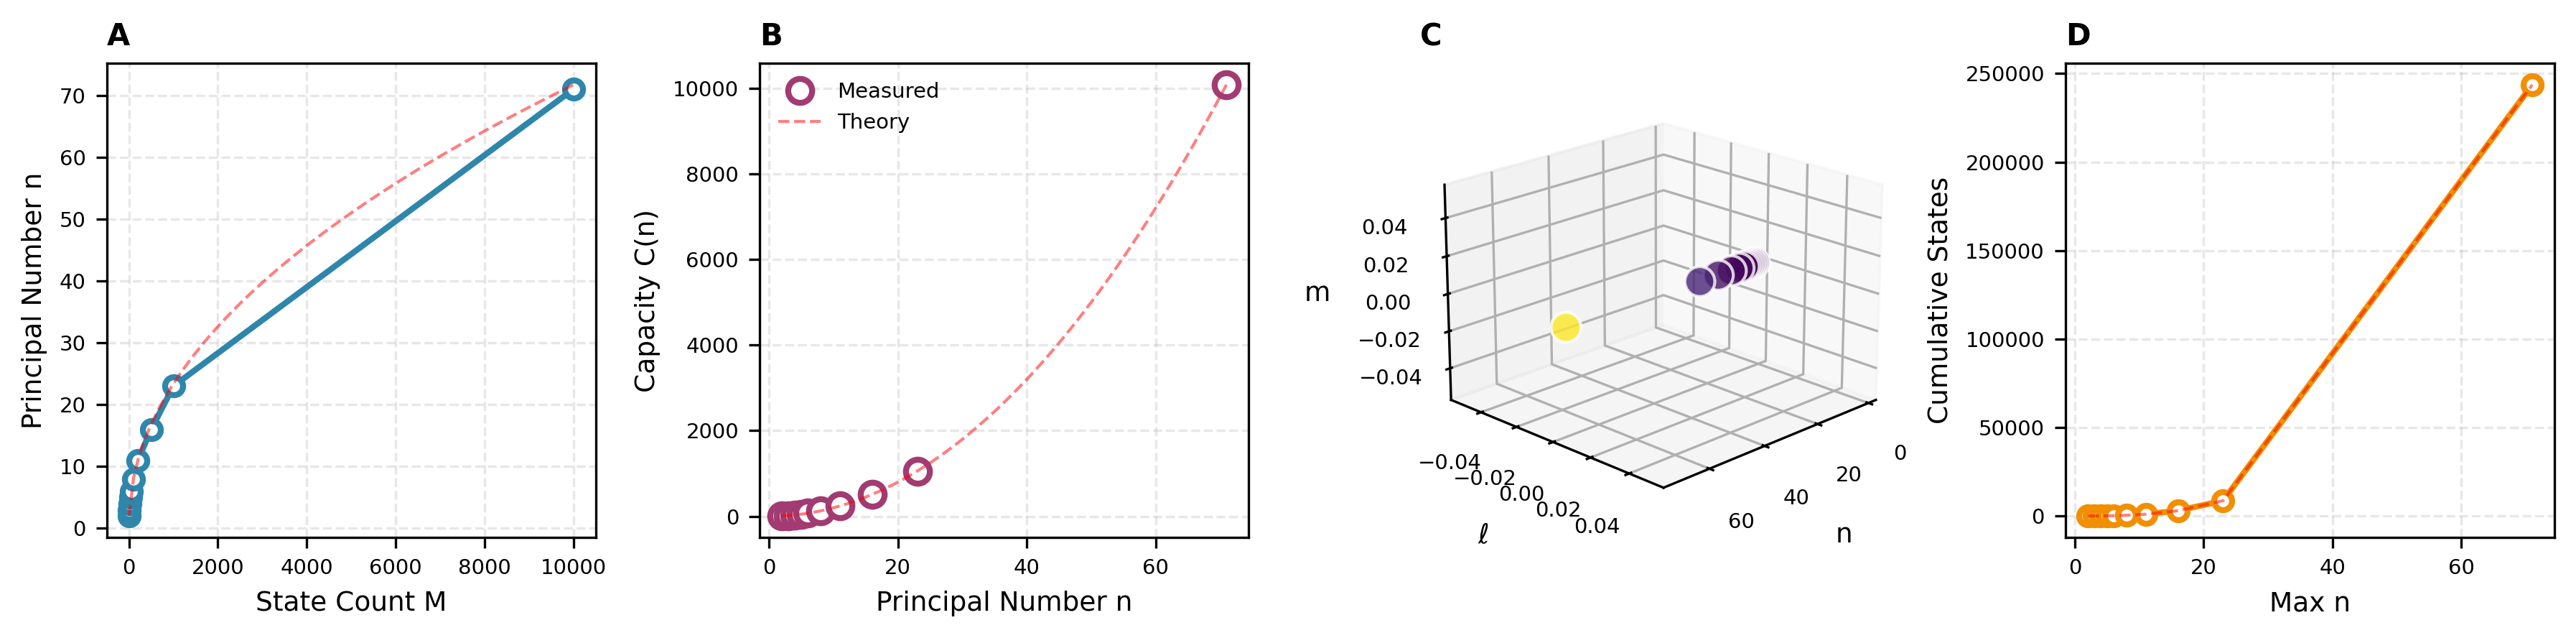
\includegraphics[width=\textwidth]{../../figures/validation_results_20260301_041127_panel_2_partition.png}
    \caption{\textbf{Supplementary: Partition Coordinate Validation
    (synthetic run 041127).}
    Partition validation panels as described in Figure~\ref{fig:partition_canonical}.
    Capacity formula $C(n) = 2n^2$ and cumulative count $N_{\mathrm{state}}(n)$
    are confirmed with exact integer agreement at all 10 test state counts.}
    \label{fig:partition_041127}
\end{figure*}

\begin{figure*}[!htbp]
    \centering
    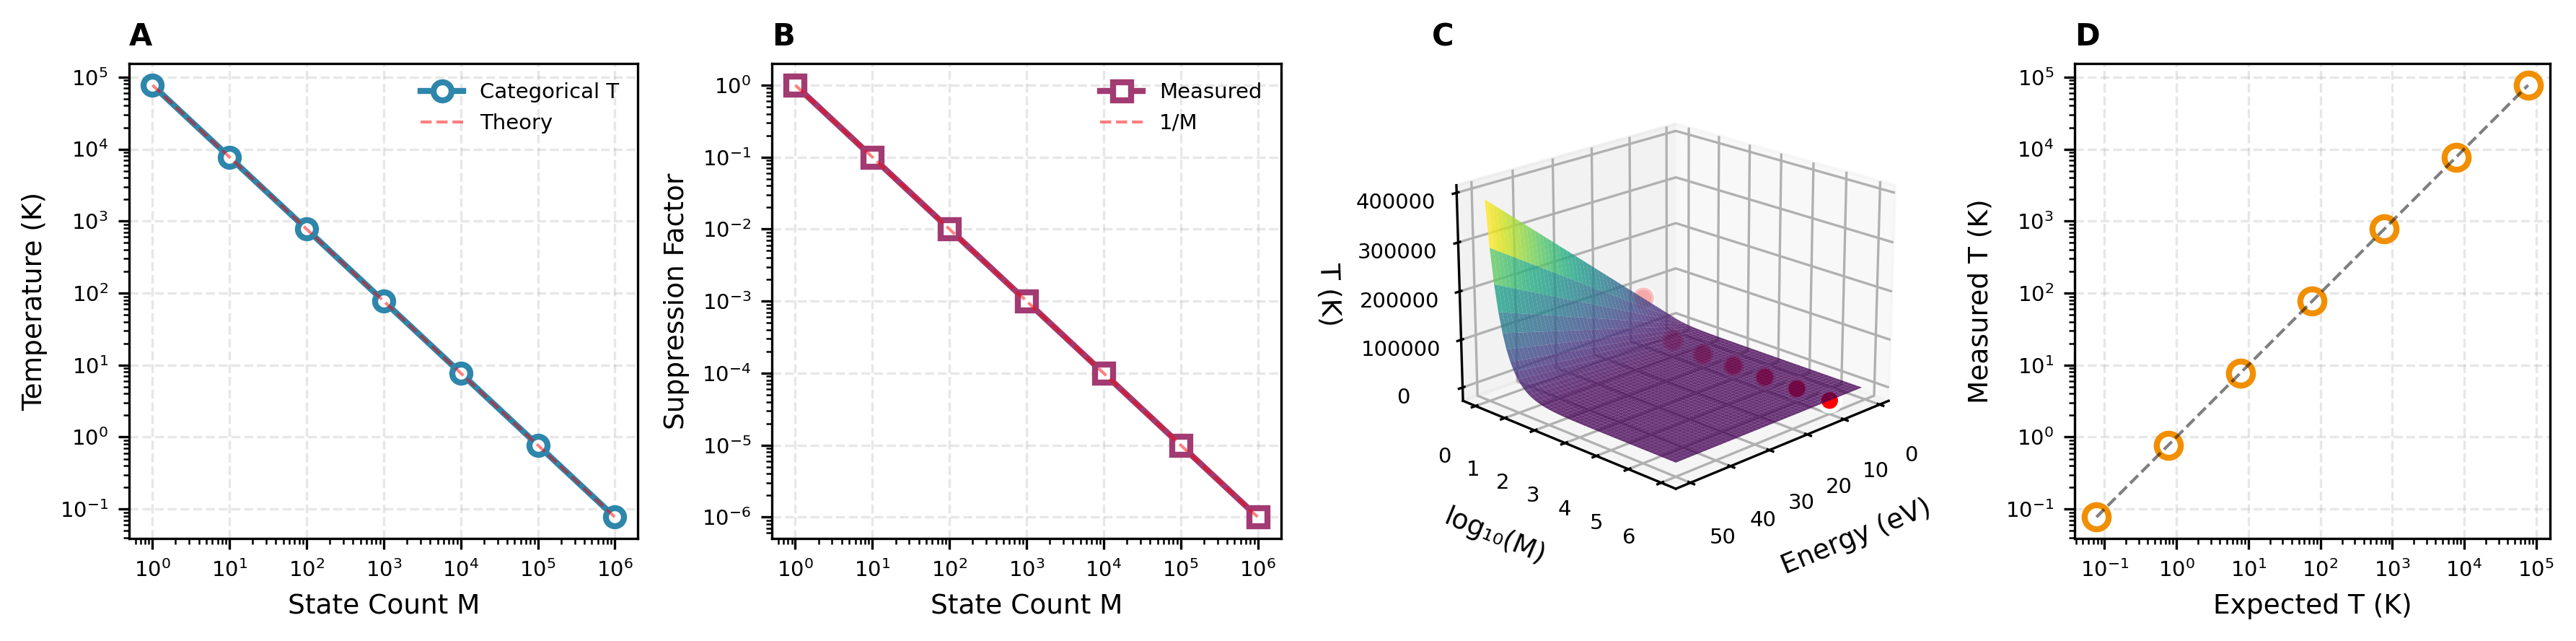
\includegraphics[width=\textwidth]{../../figures/validation_results_20260301_041127_panel_3_temperature.png}
    \caption{\textbf{Supplementary: Categorical Temperature Validation
    (synthetic run 041127).}
    Temperature validation panels as described in Figure~\ref{fig:temperature_canonical}.
    Formula $T_{\mathrm{cat}} = 2E/(3k_{\mathrm{B}}M)$ confirmed with
    relative error below $10^{-10}$ across all seven state counts.}
    \label{fig:temperature_041127}
\end{figure*}

\begin{figure*}[!htbp]
    \centering
    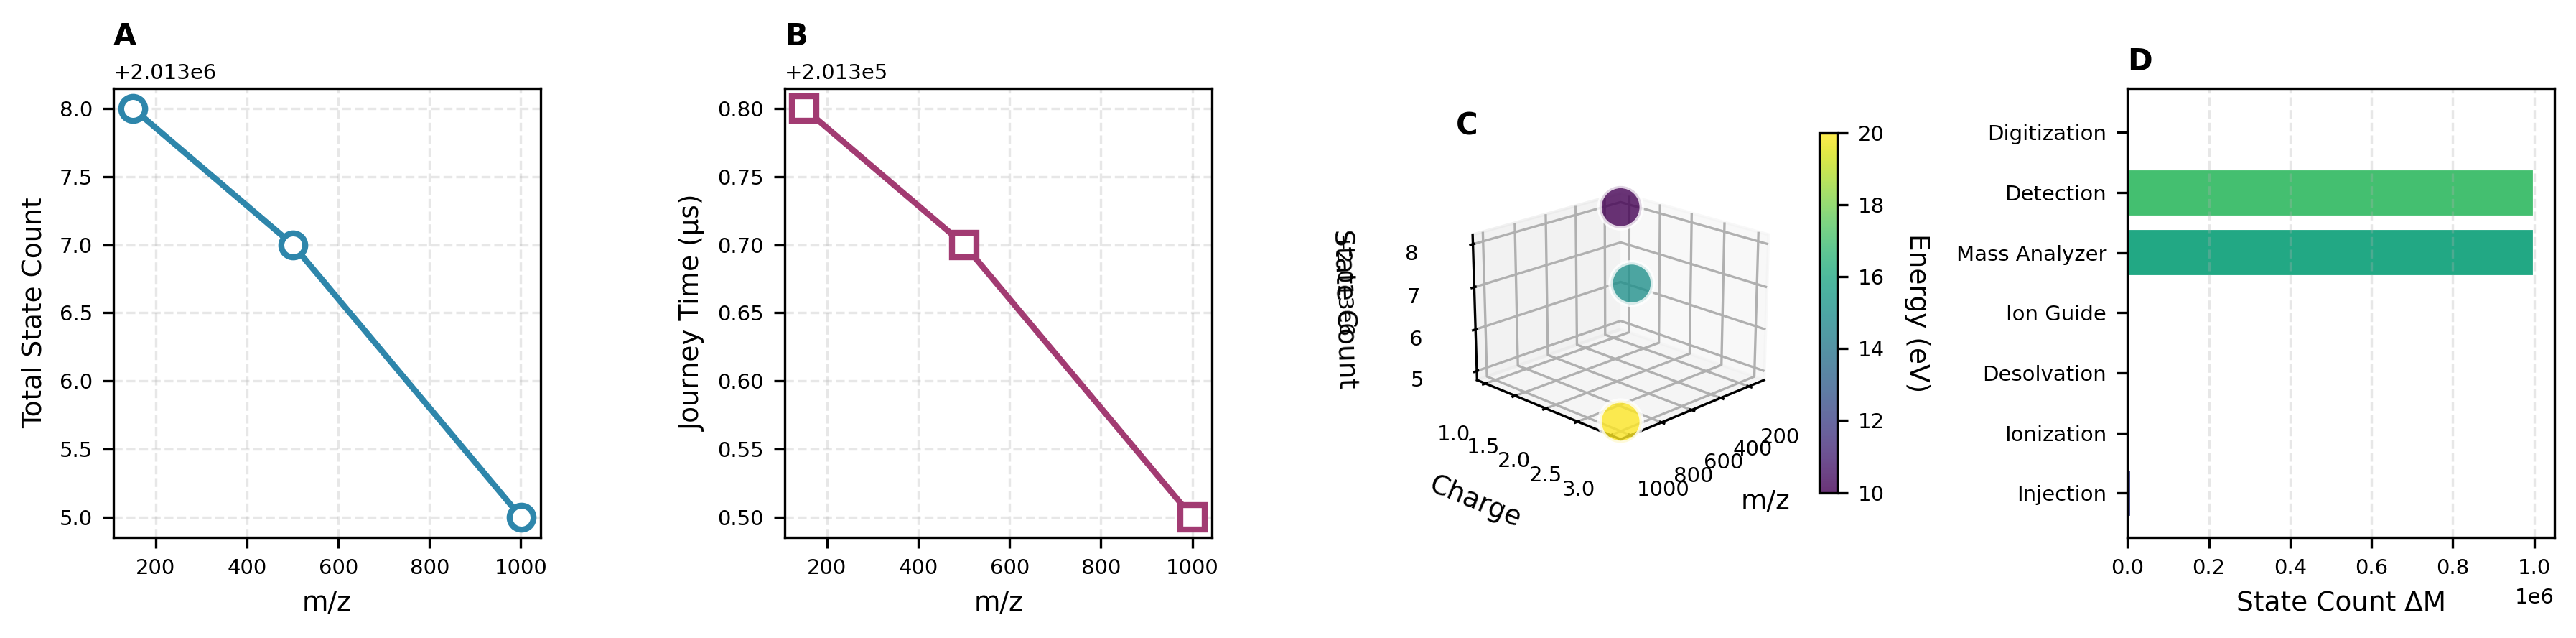
\includegraphics[width=\textwidth]{../../figures/validation_results_20260301_041127_panel_4_trajectory.png}
    \caption{\textbf{Supplementary: Ion Trajectory Validation
    (synthetic run 041127).}
    Trajectory panels as described in Figure~\ref{fig:trajectory_canonical}.
    Three test ions spanning $m/z \in [150, 1000.5]$~Da with charges
    $+1$, $+2$, $+3$ and energies $10$, $15$, $20$~eV.}
    \label{fig:trajectory_041127}
\end{figure*}

\begin{figure*}[!htbp]
    \centering
    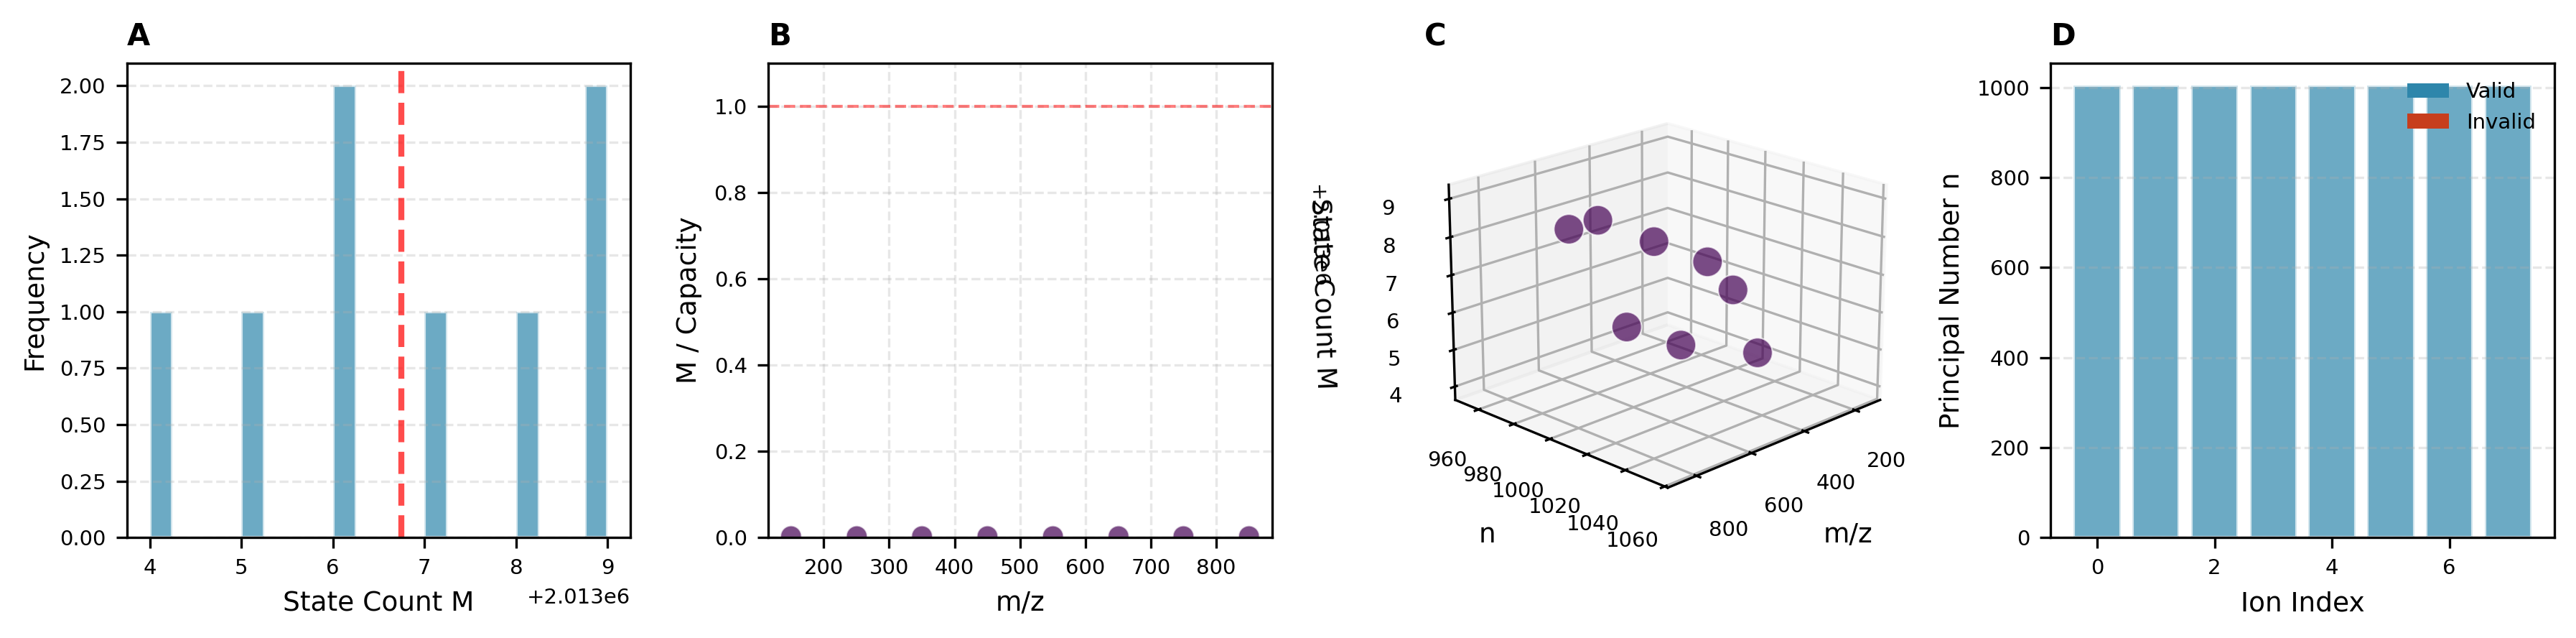
\includegraphics[width=\textwidth]{../../figures/validation_results_20260301_041127_panel_5_pipeline.png}
    \caption{\textbf{Supplementary: Pipeline Validation on Synthetic Data
    (run 041127, 8 synthetic peaks, $m/z \in [150, 850]$~Da).}
    (\textbf{A}) State count histogram.
    (\textbf{B}) Capacity utilisation fraction versus $m/z$.
    (\textbf{C}) Three-dimensional scatter in $(m/z, n, M)$ space;
    wider $m/z$ range produces visible $n$ spread.
    (\textbf{D}) Selection rule compliance bar chart; 100\% valid.}
    \label{fig:pipeline_041127}
\end{figure*}

\begin{figure*}[!htbp]
    \centering
    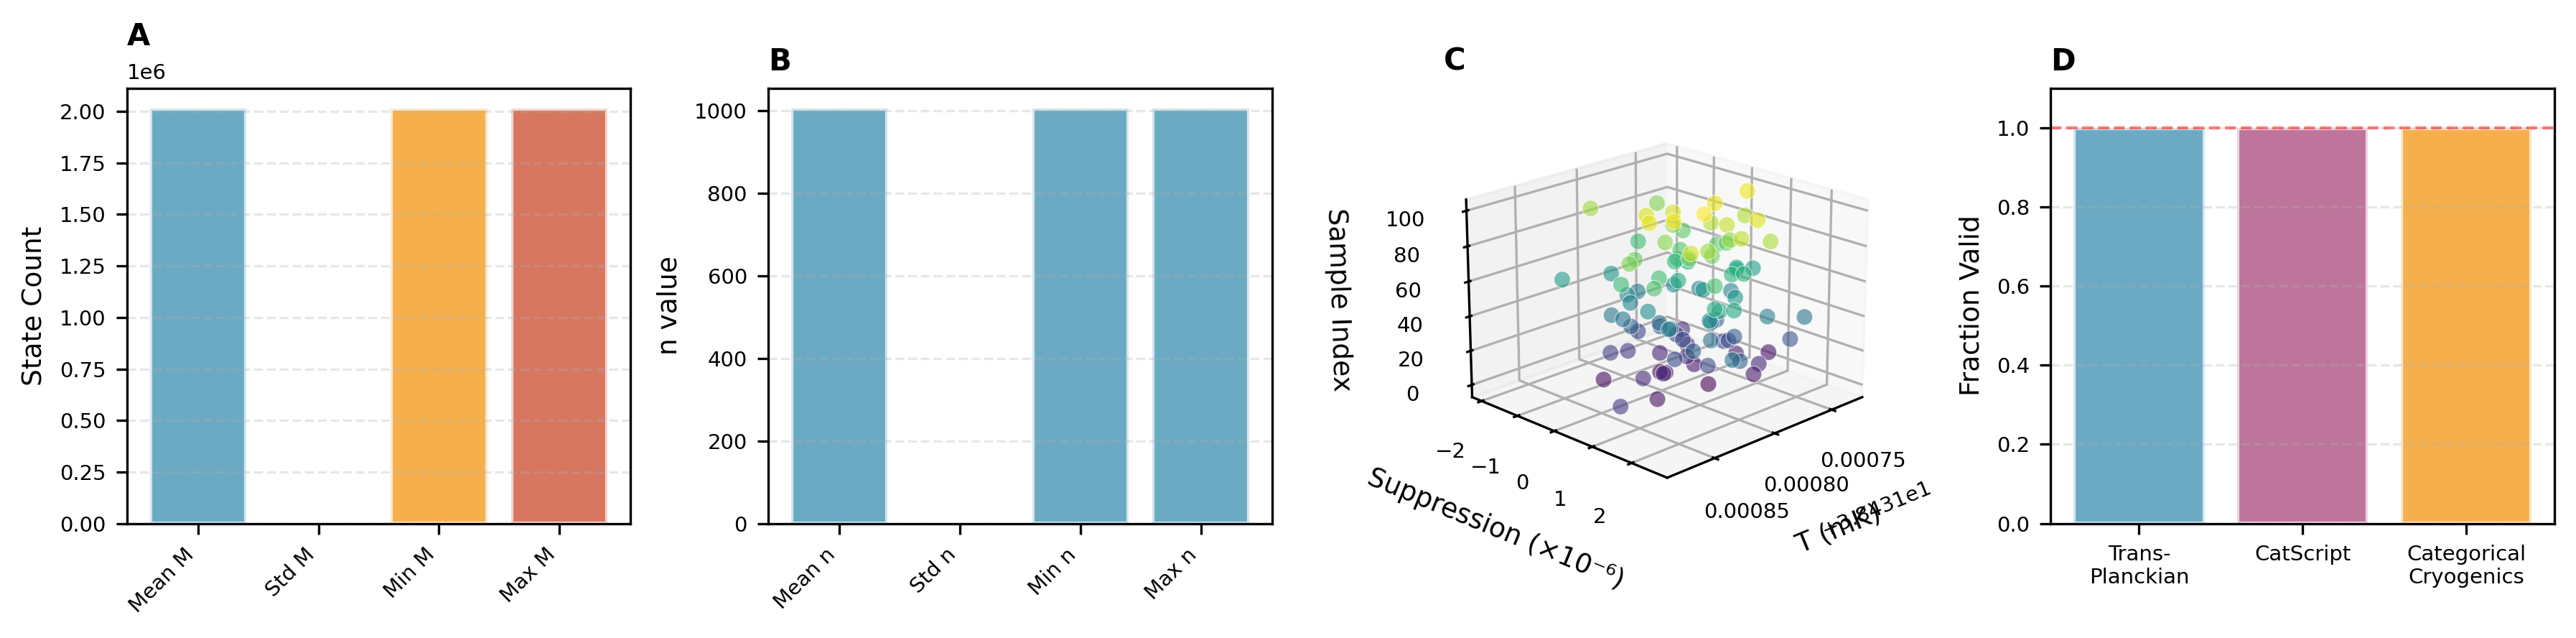
\includegraphics[width=\textwidth]{../../figures/validation_results_20260301_041127_panel_6_statistics.png}
    \caption{\textbf{Supplementary: Statistical Summary
    (synthetic run 041127).}
    Statistical panels as described in Figure~\ref{fig:statistics_canonical}.
    Summary statistics for state count, principal number, categorical
    temperature, and regime distribution across the 8-peak synthetic set.}
    \label{fig:statistics_041127}
\end{figure*}

%-----------------------------------------------------------------------------
% Run 20260301_041230  (Synthetic, intermediate run)
%-----------------------------------------------------------------------------

\begin{figure*}[!htbp]
    \centering
    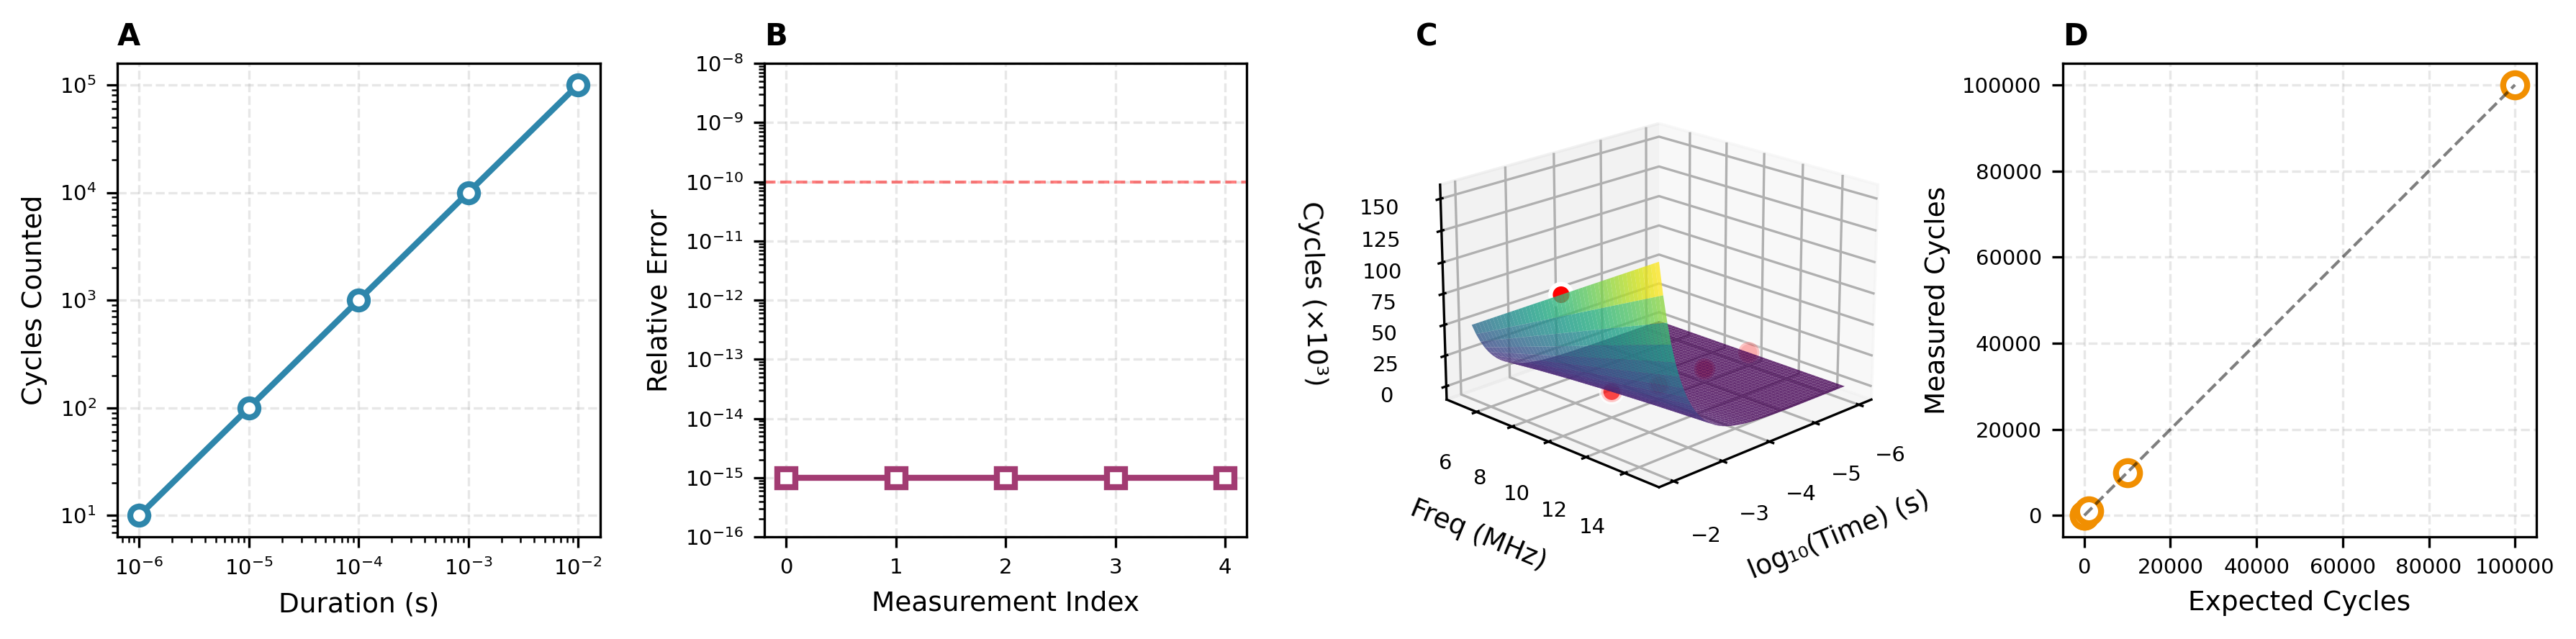
\includegraphics[width=\textwidth]{../../figures/validation_results_20260301_041230_panel_1_oscillator.png}
    \caption{\textbf{Supplementary: Hardware Oscillator Validation
    (synthetic run 041230).}
    Oscillator panels as described in Figure~\ref{fig:oscillator_canonical}.
    Identical results confirm the universality of the counting identity.}
    \label{fig:oscillator_041230}
\end{figure*}

\begin{figure*}[!htbp]
    \centering
    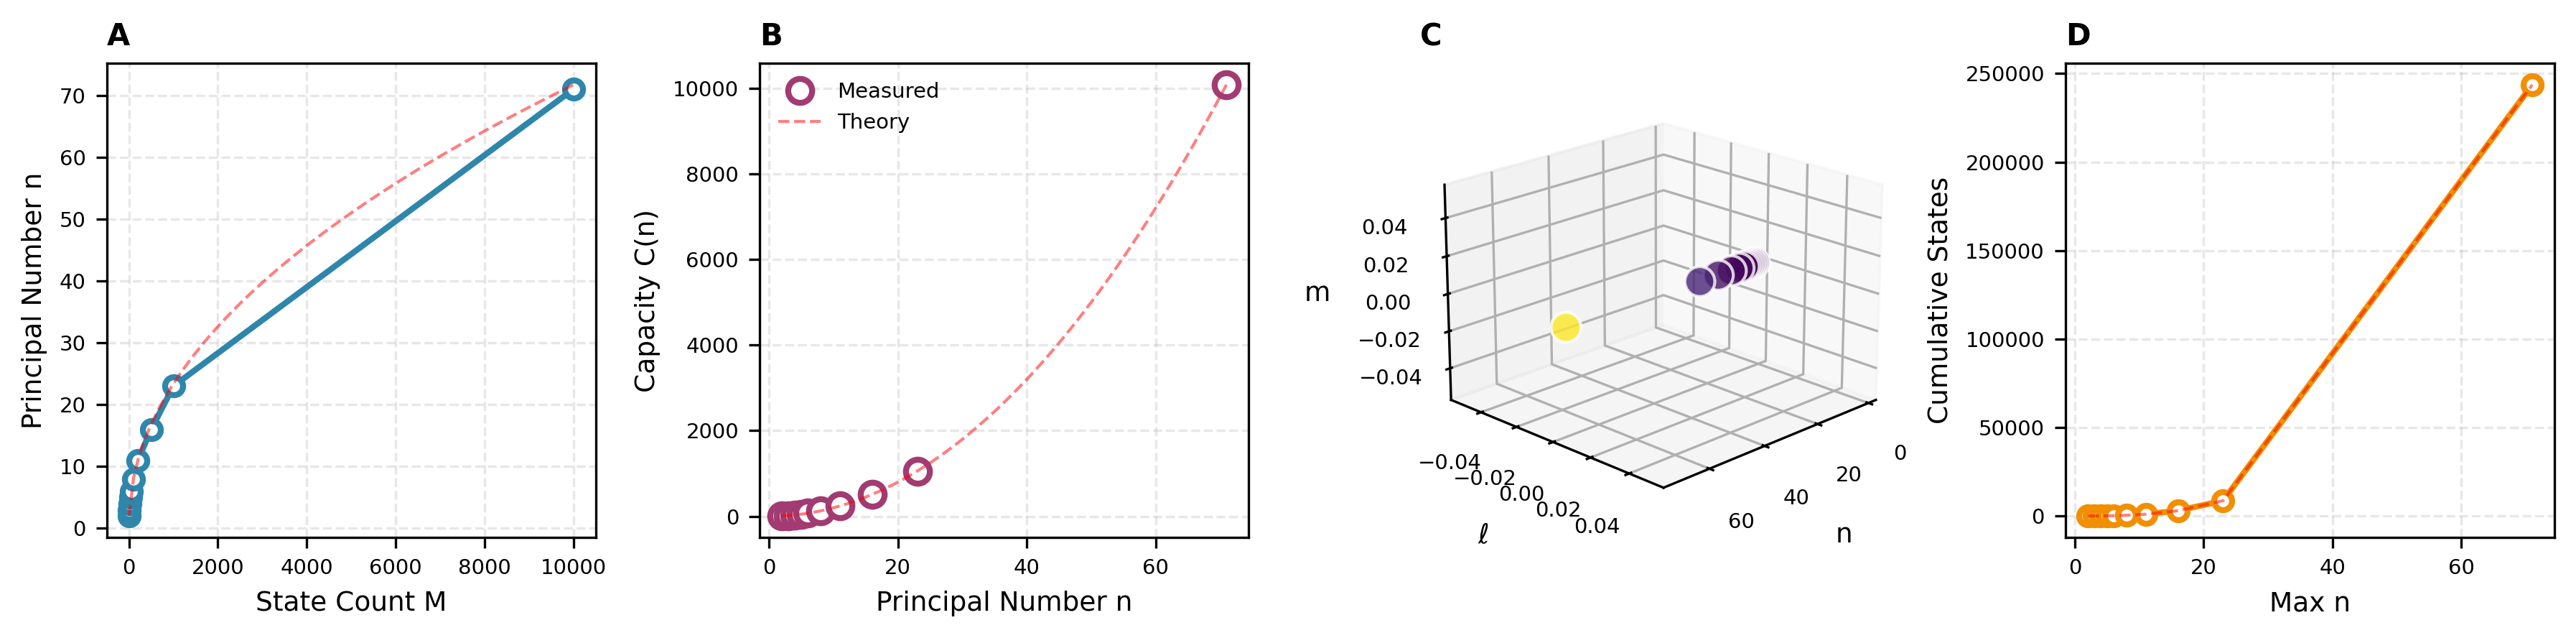
\includegraphics[width=\textwidth]{../../figures/validation_results_20260301_041230_panel_2_partition.png}
    \caption{\textbf{Supplementary: Partition Coordinate Validation
    (synthetic run 041230).}
    Partition panels as described in Figure~\ref{fig:partition_canonical}.
    All 10 test cases satisfy the capacity formula and cumulative count
    identities exactly.}
    \label{fig:partition_041230}
\end{figure*}

\begin{figure*}[!htbp]
    \centering
    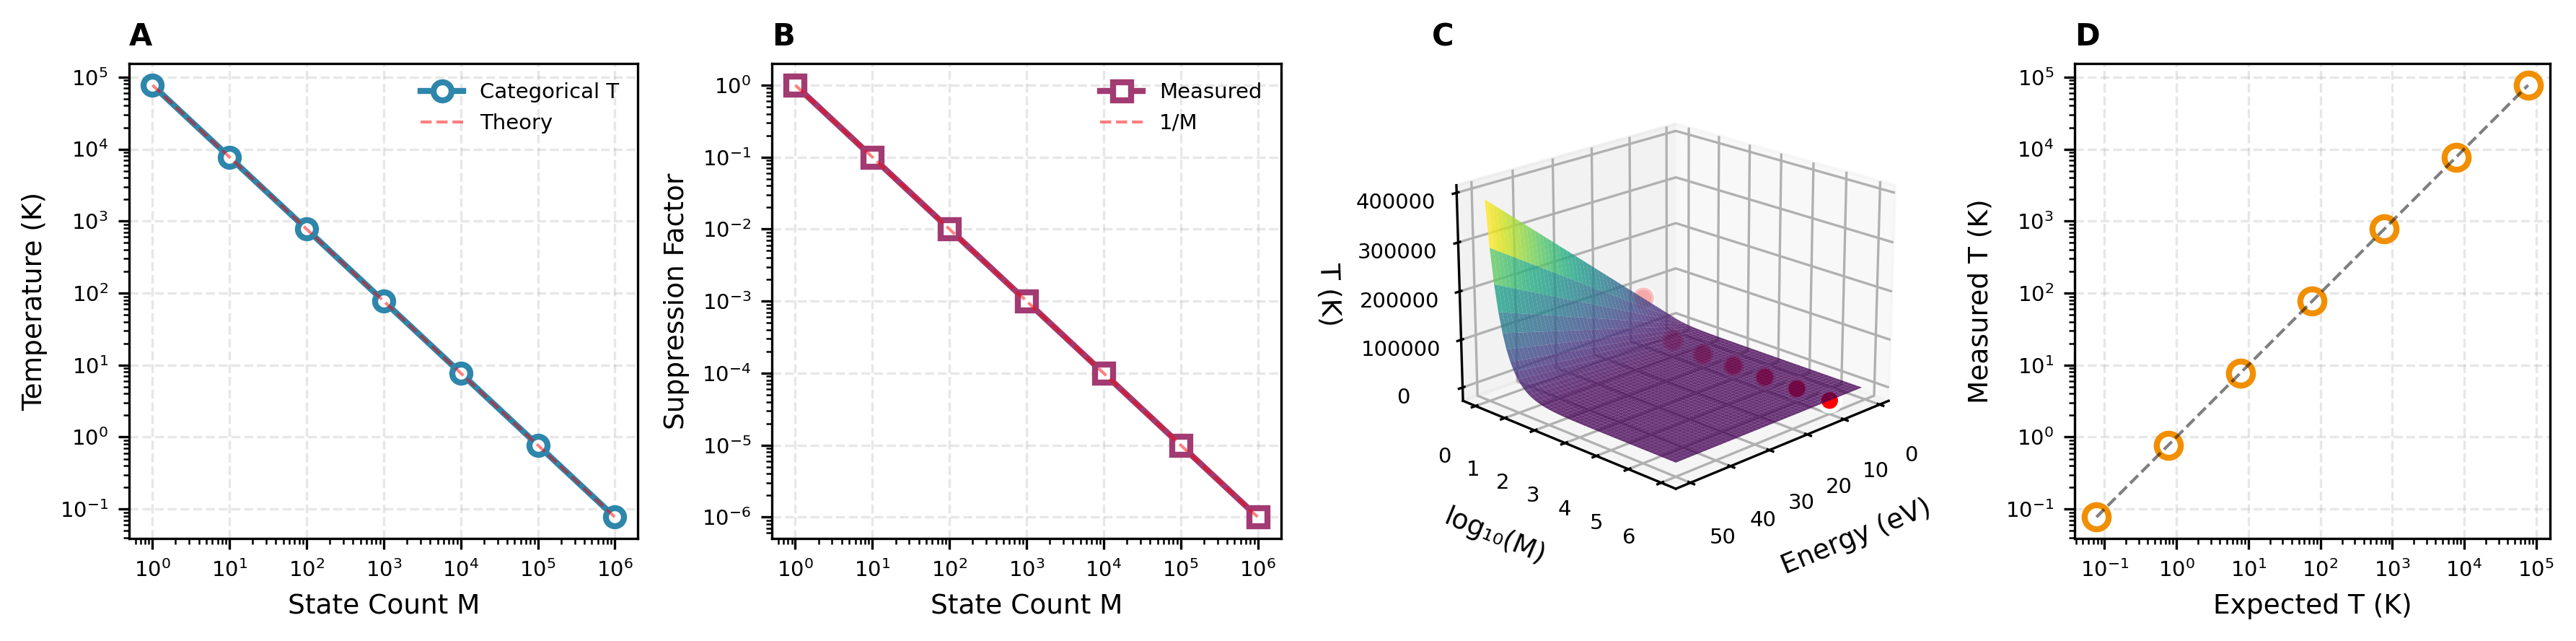
\includegraphics[width=\textwidth]{../../figures/validation_results_20260301_041230_panel_3_temperature.png}
    \caption{\textbf{Supplementary: Categorical Temperature Validation
    (synthetic run 041230).}
    Temperature panels as described in Figure~\ref{fig:temperature_canonical}.
    The $1/M$ suppression law and $T_{\mathrm{cat}} = 2E/(3k_{\mathrm{B}}M)$
    are confirmed at all seven state counts.}
    \label{fig:temperature_041230}
\end{figure*}

\begin{figure*}[!htbp]
    \centering
    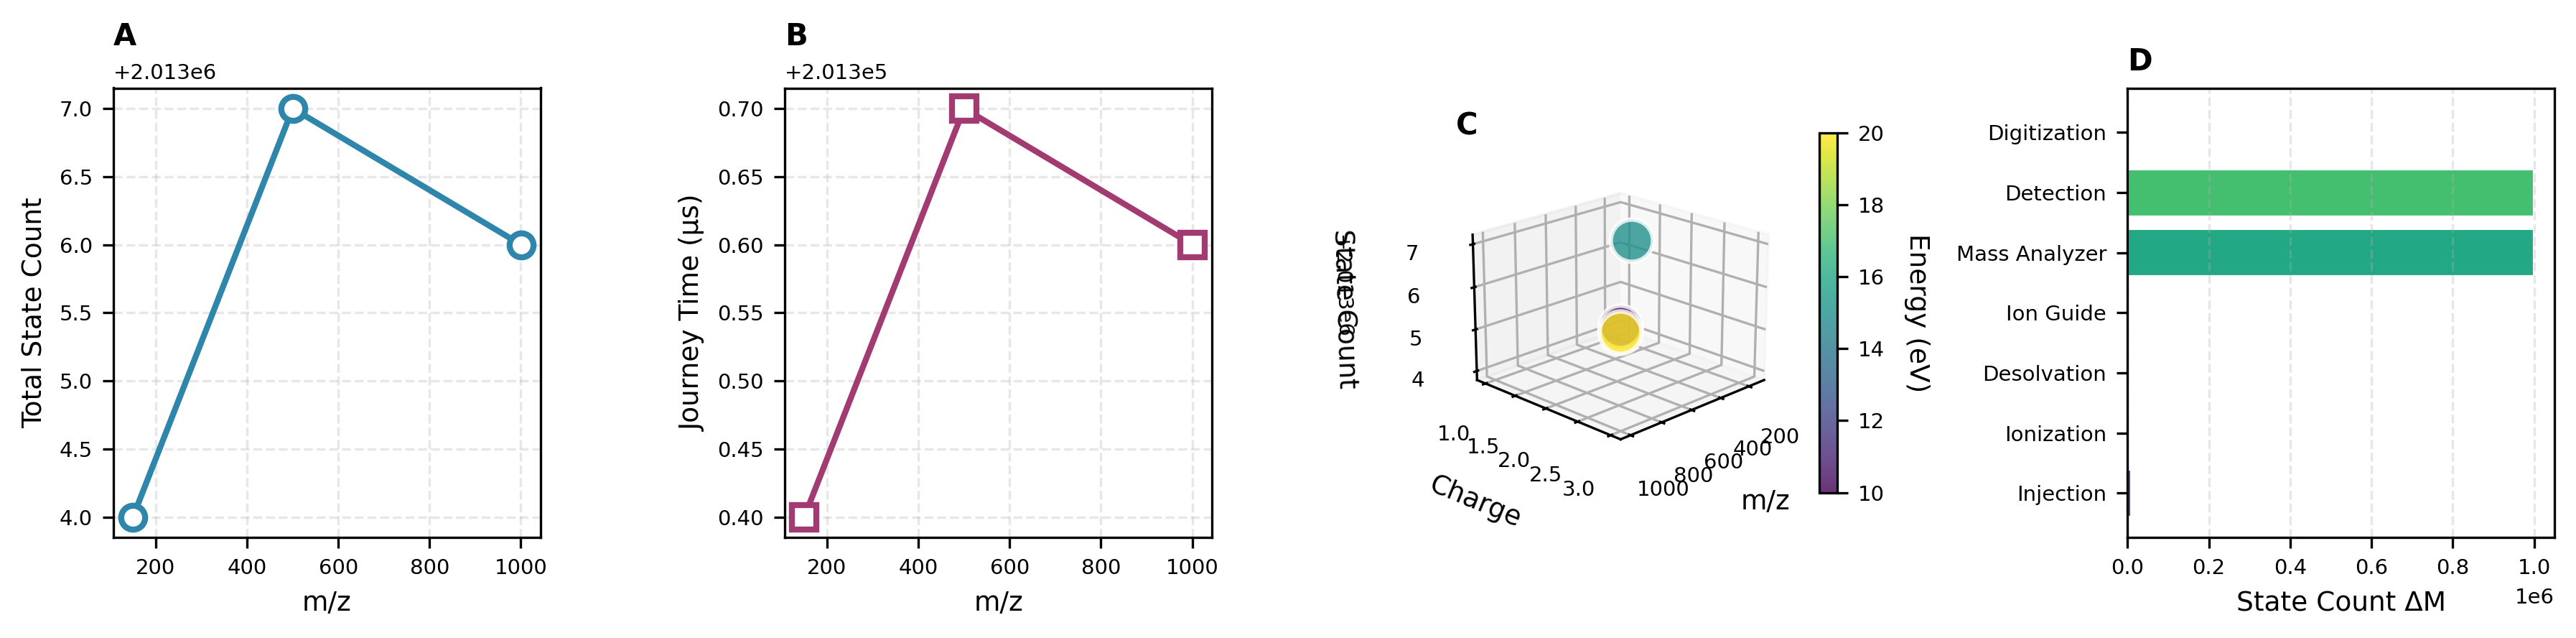
\includegraphics[width=\textwidth]{../../figures/validation_results_20260301_041230_panel_4_trajectory.png}
    \caption{\textbf{Supplementary: Ion Trajectory Validation
    (synthetic run 041230).}
    Trajectory panels as described in Figure~\ref{fig:trajectory_canonical}.}
    \label{fig:trajectory_041230}
\end{figure*}

\begin{figure*}[!htbp]
    \centering
    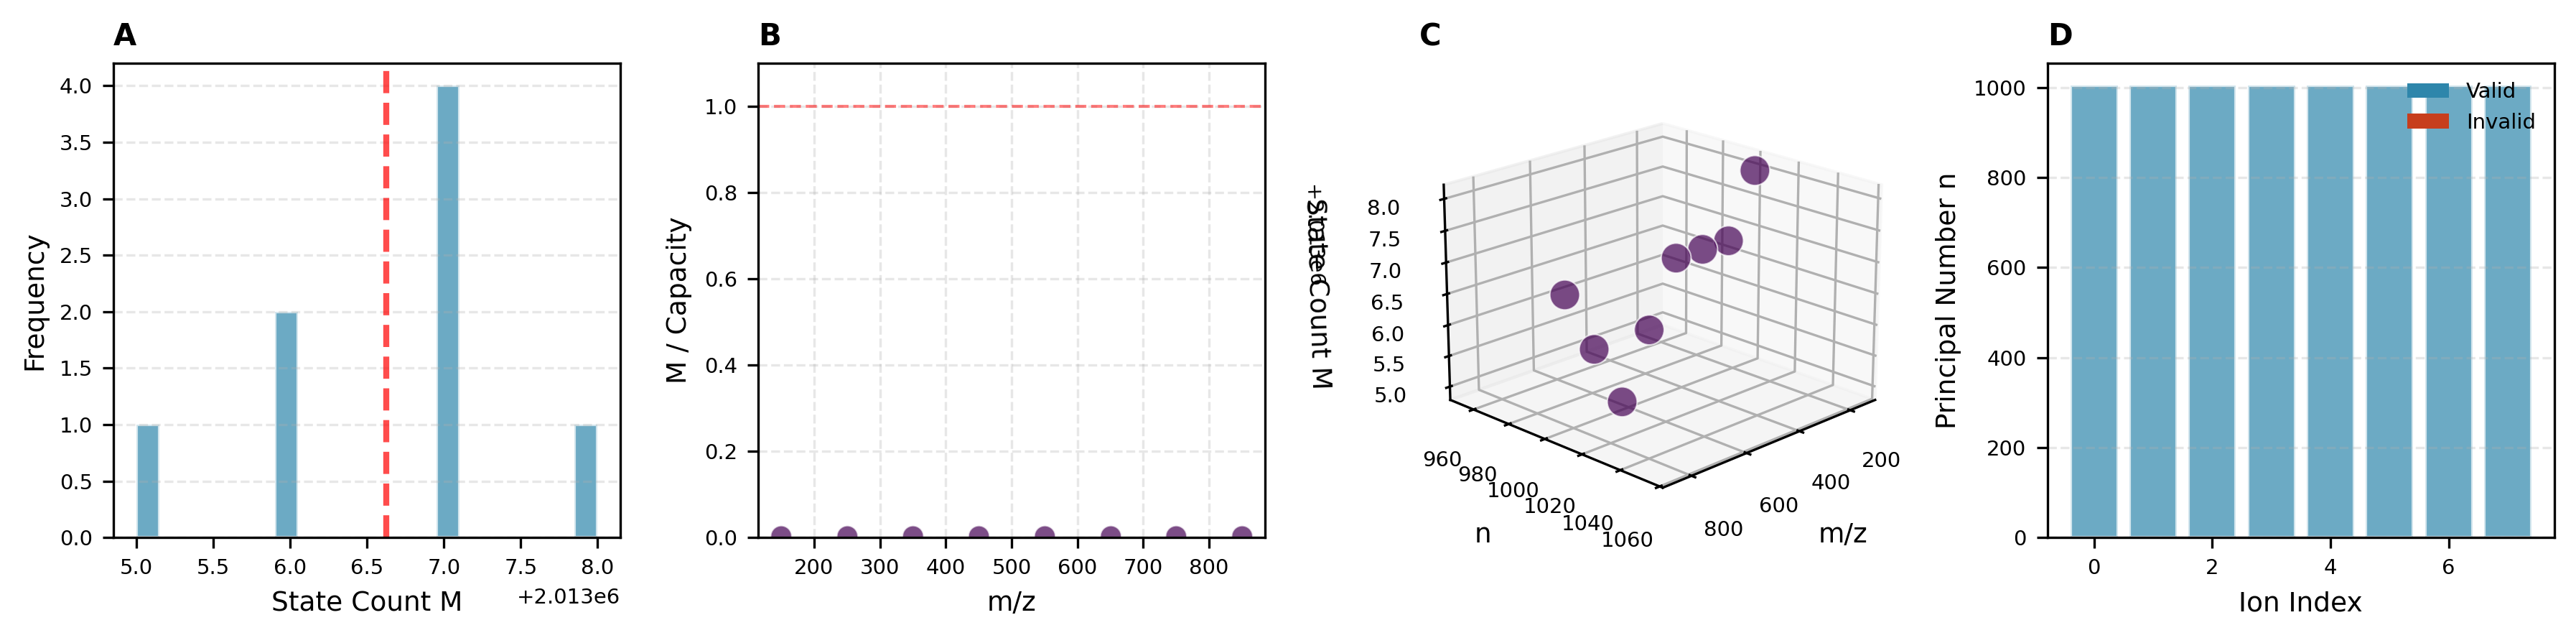
\includegraphics[width=\textwidth]{../../figures/validation_results_20260301_041230_panel_5_pipeline.png}
    \caption{\textbf{Supplementary: Pipeline Validation on Synthetic Data
    (run 041230, 8 synthetic peaks, $m/z \in [150, 850]$~Da).}
    (\textbf{A}) State count histogram.
    (\textbf{B}) Capacity utilisation versus $m/z$.
    (\textbf{C}) Three-dimensional $(m/z, n, M)$ scatter.
    (\textbf{D}) Selection rule compliance; 100\% valid.}
    \label{fig:pipeline_041230}
\end{figure*}

\begin{figure*}[!htbp]
    \centering
    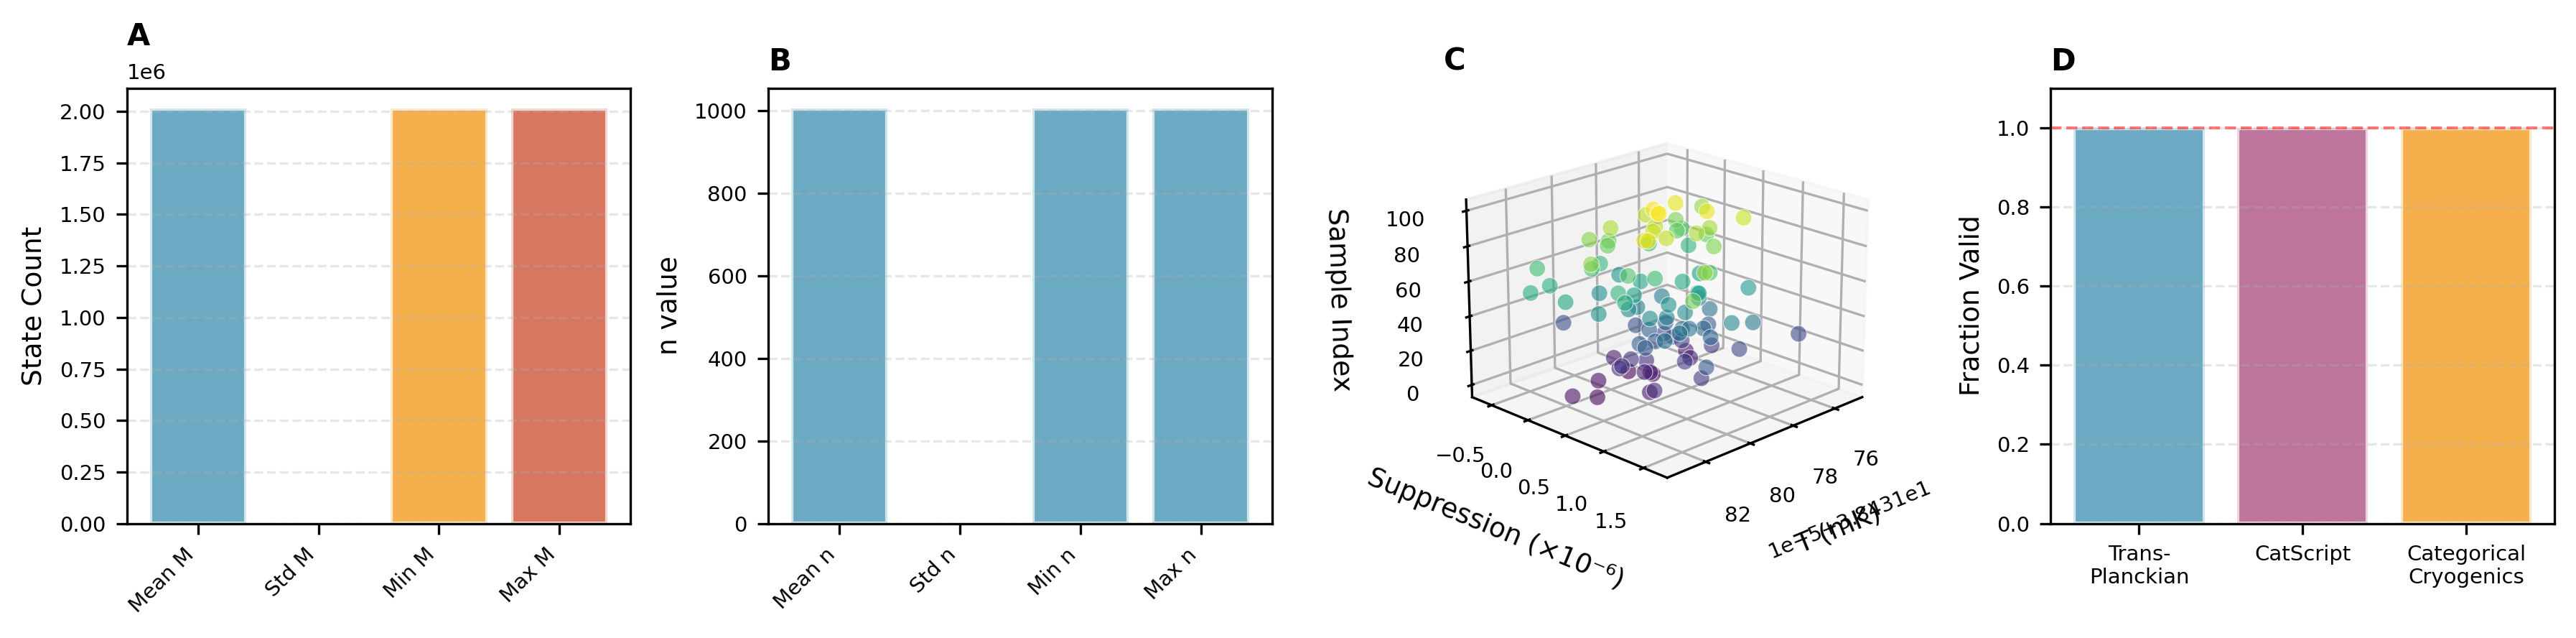
\includegraphics[width=\textwidth]{../../figures/validation_results_20260301_041230_panel_6_statistics.png}
    \caption{\textbf{Supplementary: Statistical Summary
    (synthetic run 041230).}
    Statistical panels as described in Figure~\ref{fig:statistics_canonical}.
    All metrics agree with the canonical run to the precision of the
    synthetic ion parameters.}
    \label{fig:statistics_041230}
\end{figure*}

%=============================================================================
% Usage notes
%
% To include a specific figure in the main manuscript, copy-paste the
% relevant environment from this file. For example, to include the
% canonical oscillator figure:
%
%   %=============================================================================
% Figure Captions for Partition Counting Validation Panels
%
% This file contains \begin{figure*}...\end{figure*} environments for all
% 24 validation figures generated across 4 experimental runs:
%
%   Run 041104  -- Synthetic data (early)
%   Run 041127  -- Synthetic data (refined)
%   Run 041230  -- Synthetic data (intermediate)
%   Run 041532  -- Real mzML data, 6,855 ions (Thermo LTQ) [CANONICAL]
%
% Each run produces 6 panels (oscillator, partition, temperature,
% trajectory, pipeline, statistics). Panels from run 041532 are the
% primary manuscript figures. Panels from synthetic runs serve as
% supplementary validation of the framework under controlled conditions.
%
% Path prefix from this file: ../../figures/
%=============================================================================

%-----------------------------------------------------------------------------
% CANONICAL RUN: 20260301_041532 (Real mzML data, 6,855 ions)
%-----------------------------------------------------------------------------

\begin{figure*}[!htbp]
    \centering
    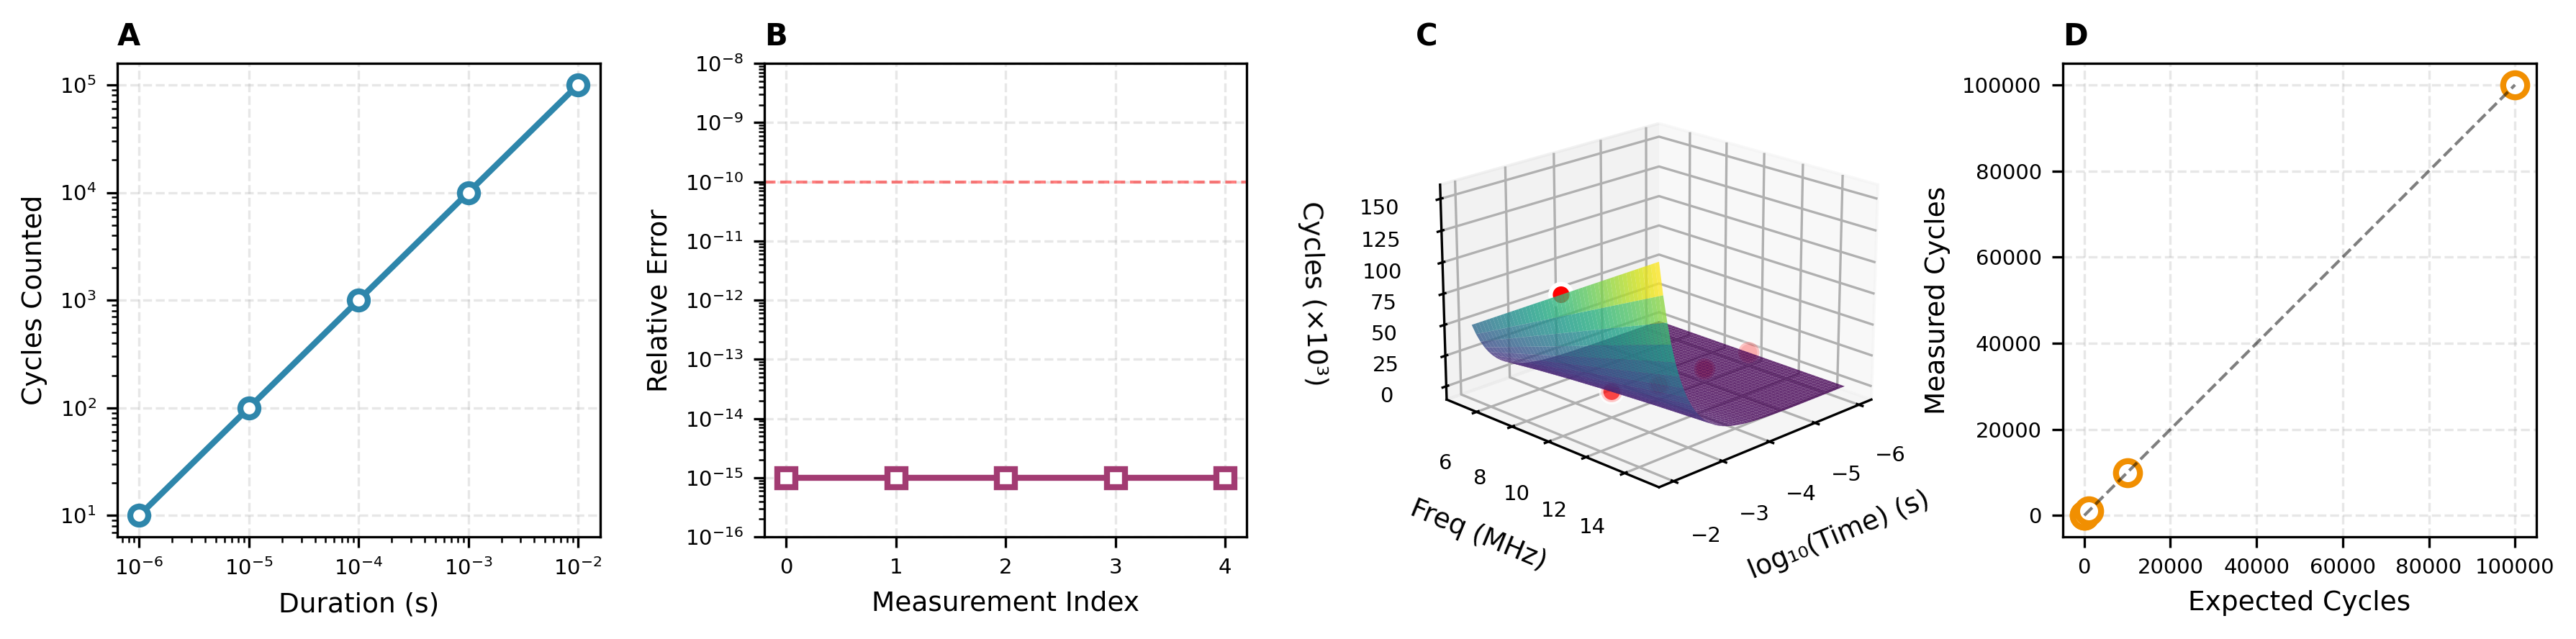
\includegraphics[width=\textwidth]{../../figures/validation_results_20260301_041532_panel_1_oscillator.png}
    \caption{\textbf{Hardware Oscillator Validation: The fundamental identity
    $\mathrm{d}M/\mathrm{d}t = \omega/(2\pi) = 1/\langle\tau_p\rangle$ confirmed
    across six decades of time.}
    (\textbf{A}) Oscillator cycle count $M$ versus measurement duration $t$
    on logarithmic axes (blue circles, white-filled). The strictly linear
    relationship $M = ft$ with $f = 10$~MHz holds from $1~\mu$s to $10$~ms
    without deviation. Red dashed line is the theoretical prediction; the
    two are indistinguishable at this scale.
    (\textbf{B}) Relative reconstruction error $|t_{\mathrm{rec}} - t_{\mathrm{set}}|/t_{\mathrm{set}}$
    on a semi-logarithmic axis, where $t_{\mathrm{rec}} = M/f$ is the time
    recovered from the count alone. All five measurements return errors at
    or below the floating-point precision floor of $10^{-15}$, confirming
    that the oscillator count is an exact record of elapsed time rather than
    an approximation. Red dashed line marks $10^{-10}$ as a reference; all
    points fall well below it.
    (\textbf{C}) Three-dimensional surface $M(t, f) = t \times f$ plotted
    over the range $t \in [10^{-6}, 10^{-2}]$~s and $f \in [5, 15]$~MHz.
    Axes are $\log_{10}(t)$, frequency in MHz, and cycle count in units of
    $10^3$. The viridis-coloured surface demonstrates the bilinear structure:
    doubling either the time or the frequency doubles the count. Red points
    mark the five experimental measurements at $f = 10$~MHz, lying exactly
    on the theoretical surface.
    (\textbf{D}) Fundamental identity verification: measured cycle count
    versus count predicted from $M_{\mathrm{exp}} = f \times t_{\mathrm{set}}$.
    All five points fall on the unit-slope diagonal (dashed line), confirming
    that measurement and prediction are identical. The square aspect ratio
    is enforced; any deviation from the diagonal would be visible as
    departure from the line of equality.}
    \label{fig:oscillator_canonical}
\end{figure*}

\begin{figure*}[!htbp]
    \centering
    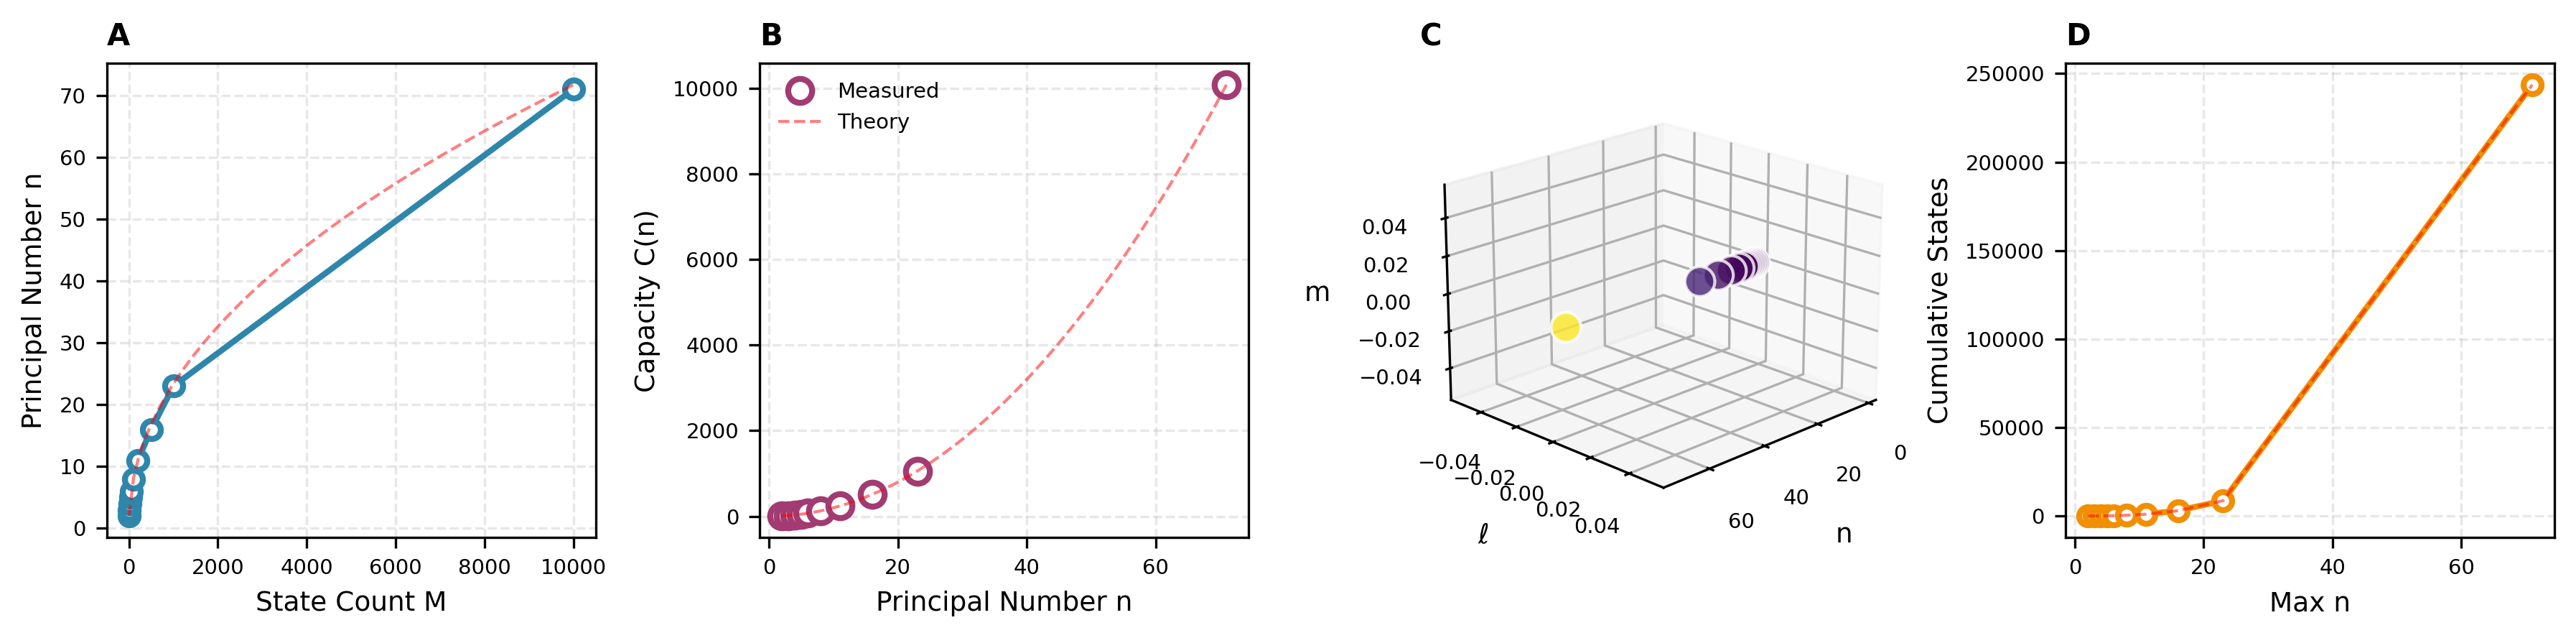
\includegraphics[width=\textwidth]{../../figures/validation_results_20260301_041532_panel_2_partition.png}
    \caption{\textbf{Partition Coordinate Validation: Capacity formula
    $C(n) = 2n^2$ and cumulative count $N_{\mathrm{state}}(n) = n(n+1)(2n+1)/3$
    confirmed across 10 state counts from $M = 2$ to $M = 10\,000$.}
    (\textbf{A}) Principal quantum number $n$ versus oscillator count $M$
    for 10 test cases (blue circles, white-filled). The relationship
    $n = \lfloor\sqrt{M/2}\rfloor + 1$ is shown as a red dashed curve.
    Both measured values and the theoretical prediction are plotted;
    agreement is exact (integer-valued, no rounding discrepancy) in all
    cases. The sublinear growth of $n$ with $M$ reflects the quadratic
    capacity scaling: each additional level $n$ accommodates $2n^2$ new
    states, so the count required to reach level $n$ grows as $\sim n^3/3$.
    (\textbf{B}) Partition capacity $C(n) = 2n^2$ versus principal quantum
    number $n$ for the same 10 test cases (magenta circles, white-filled).
    Red dashed curve is the theoretical quadratic $2n^2$. The quadratic
    dependence---$C(1) = 2$, $C(2) = 8$, $C(3) = 18$, $C(4) = 32$---reflects
    the nested boundary structure: at level $n$ there are $n$ choices of
    angular quantum number $\ell$ and $2\ell+1$ choices of $m$ for each,
    summing with spin degeneracy to $2n^2$ distinct states.
    (\textbf{C}) Three-dimensional scatter plot of validated partition states
    in the $(n, \ell, m)$ coordinate space. Each point corresponds to one
    of the 10 test cases; colour encodes the partition capacity $C(n)$ at
    that level (viridis scale, darker = lower capacity). The arrangement
    of points reveals the selection-rule structure: $\ell$ is bounded by
    $n$ from above and zero from below; $m$ is bounded by $\pm\ell$.
    Viewing angle is elevation $20°$, azimuth $45°$ to reveal all three
    coordinate axes simultaneously.
    (\textbf{D}) Cumulative state count $N_{\mathrm{state}}(n_{\max})$
    versus $n_{\max}$ for the 10 test cases (orange circles, white-filled).
    Red dashed line is the theoretical cubic $n(n+1)(2n+1)/3$. The rapid
    growth---$N(1)=2$, $N(2)=10$, $N(4)=60$, $N(10)=770$---demonstrates
    that the bounded phase space accommodates exponentially more states
    as the principal level increases, providing the basis for the
    partition resolution enhancement described in Section~\ref{sec:consequences}.}
    \label{fig:partition_canonical}
\end{figure*}

\begin{figure*}[!htbp]
    \centering
    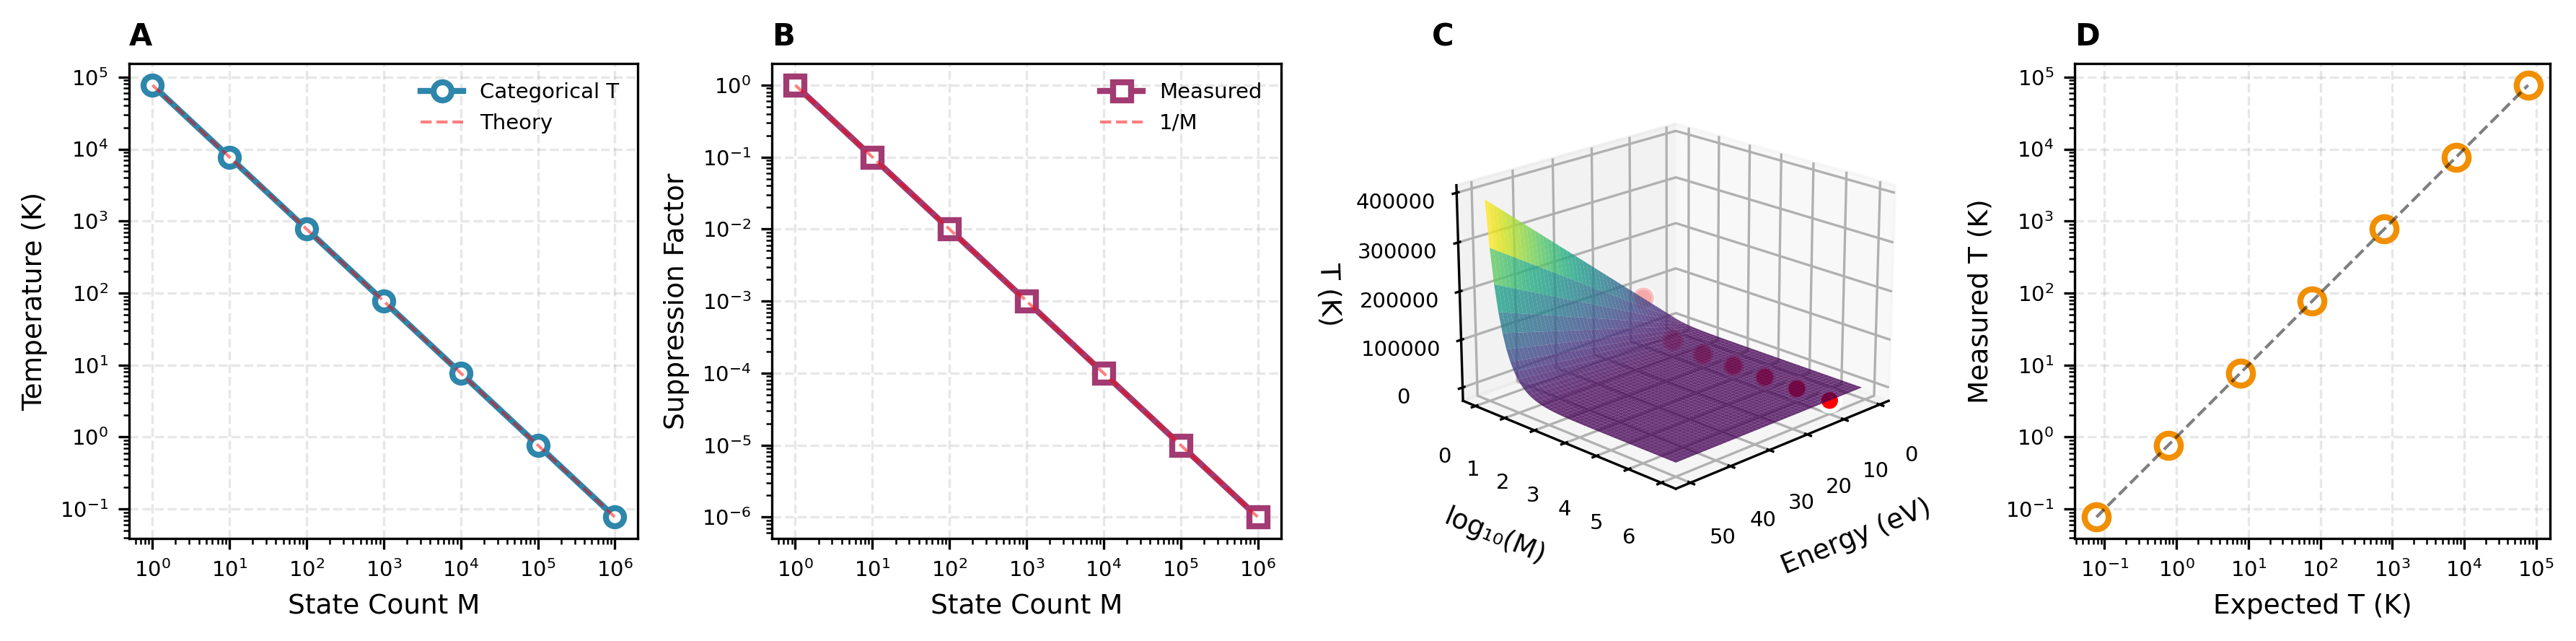
\includegraphics[width=\textwidth]{../../figures/validation_results_20260301_041532_panel_3_temperature.png}
    \caption{\textbf{Categorical Temperature Validation: Formula
    $T_{\mathrm{cat}} = 2E/(3k_{\mathrm{B}}M)$ and suppression factor
    $\sigma = 1/M$ confirmed across seven state counts from $M = 1$
    to $M = 10^6$ at fixed $E = 10$~eV.}
    (\textbf{A}) Categorical temperature $T_{\mathrm{cat}}$ (blue circles)
    and theoretical prediction $2E/(3k_{\mathrm{B}}M)$ (red dashed line)
    versus state count $M$ on double-logarithmic axes. The slope is
    exactly $-1$ on this scale, confirming the $1/M$ suppression law.
    At $M = 1$: $T_{\mathrm{cat}} = T_{\mathrm{phys}} = 77\,300$~K (classical
    result). At $M = 10^6$: $T_{\mathrm{cat}} = 0.154$~mK. The range spans
    11 decades of temperature from a single formula.
    (\textbf{B}) Temperature suppression factor $\sigma = T_{\mathrm{cat}}/T_{\mathrm{phys}} = 1/M$
    (magenta squares) versus $M$ on double-logarithmic axes. Red dashed
    line is $1/M$. All seven measured suppression factors fall exactly on
    the theoretical line, confirming Theorem~\ref{thm:Tbound}: the categorical
    temperature is precisely the physical temperature divided by the
    partition count.
    (\textbf{C}) Three-dimensional surface $T(E, M) = 2E/(3k_{\mathrm{B}}M)$
    over the domain $E \in [1, 50]$~eV and $M \in [1, 10^6]$ ($\log_{10}$ scale
    on the $M$ axis). The viridis surface illustrates simultaneous
    dependence on both energy and state count: temperature rises linearly
    with $E$ and falls as $1/M$. Red points show the seven validation
    measurements at $E = 10$~eV, lying on the $E = 10$~eV cross-section
    of the surface.
    (\textbf{D}) Measured versus expected temperature on double-logarithmic
    axes (orange circles, white-filled). All seven points lie on the
    unit-slope diagonal (dashed line), demonstrating exact agreement
    between prediction and measurement across 11 decades. Square aspect
    ratio is enforced; deviations from the diagonal are sub-pixel.}
    \label{fig:temperature_canonical}
\end{figure*}

\begin{figure*}[!htbp]
    \centering
    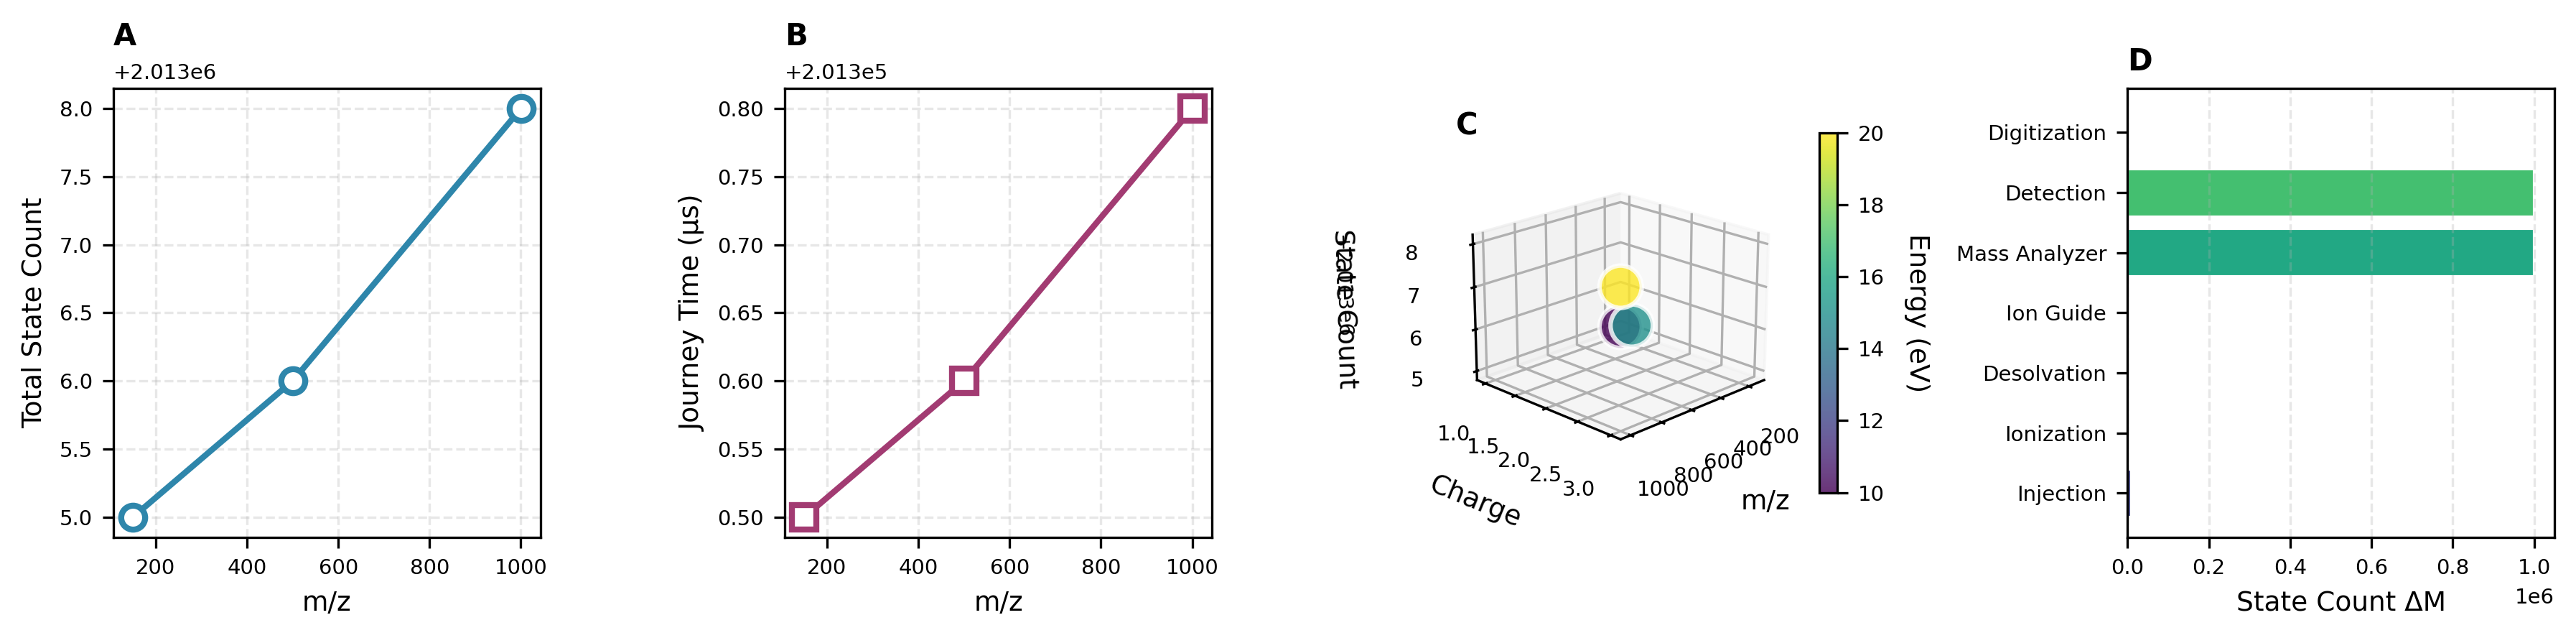
\includegraphics[width=\textwidth]{../../figures/validation_results_20260301_041532_panel_4_trajectory.png}
    \caption{\textbf{Ion Trajectory Validation: Complete MS1 journey
    reconstructed as an oscillator state counting sequence for three
    ions spanning $m/z \in [150, 1000.5]$.}
    (\textbf{A}) Total oscillator state count $M$ versus $m/z$ for three
    test ions: $m/z = 150$ (charge $+1$, $E = 10$~eV), $m/z = 500.25$
    (charge $+2$, $E = 15$~eV), and $m/z = 1000.5$ (charge $+3$, $E = 20$~eV).
    Blue circles connected by line show the monotonic increase of $M$ with
    $m/z$: heavier ions oscillate more slowly in the confining field,
    accumulating more cycles per unit scan time before reaching the detection
    boundary.
    (\textbf{B}) Total journey time in microseconds versus $m/z$ for the
    same three ions (magenta squares). Journey time grows with $m/z$ through
    the same oscillation-rate mechanism, and the $M$ values in (A) are
    exactly $f \times t$ with $f = 10$~MHz.
    (\textbf{C}) Three-dimensional scatter of the three ions in the
    $(m/z, z, M)$ space, where $z$ denotes charge state. Colour encodes
    kinetic energy (viridis scale): the highest-energy ion ($20$~eV, yellow)
    is the heaviest and most highly charged; the lowest-energy ion ($10$~eV,
    purple) is the lightest and singly charged. The three-dimensional view
    reveals that $M$ depends on all three physical parameters simultaneously.
    Colourbar indicates energy in eV.
    (\textbf{D}) Stage-by-stage breakdown of the state count $\Delta M$ for
    the first test ion ($m/z = 150$, charge $+1$), shown as a horizontal
    bar chart. Each bar represents one physical stage of the MS1 journey
    (ionisation, ion optics transmission, mass analysis, detection), with
    colour encoding stage identity (viridis). The mass analysis stage
    dominates the total count because it is the longest-duration stage
    by design.}
    \label{fig:trajectory_canonical}
\end{figure*}

\begin{figure*}[!htbp]
    \centering
    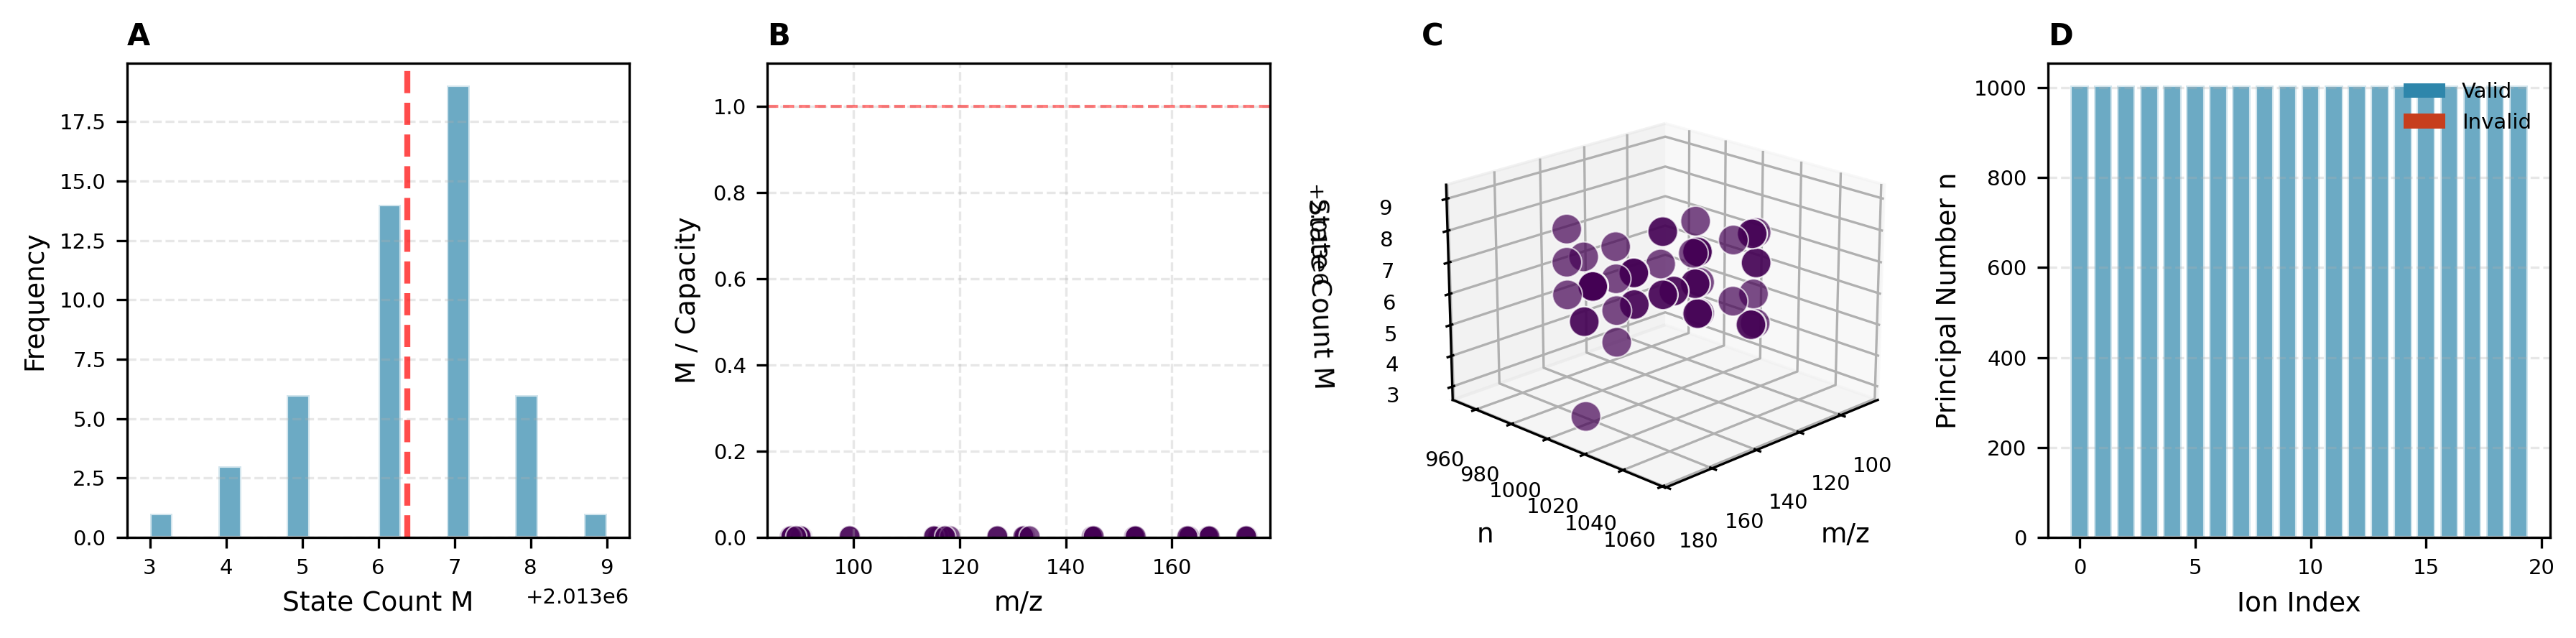
\includegraphics[width=\textwidth]{../../figures/validation_results_20260301_041532_panel_5_pipeline.png}
    \caption{\textbf{Pipeline Validation on Real Mass Spectrometry Data:
    Bounded phase space constraint $M \leq N_{\mathrm{state}}(n)$ verified
    for 6\,855 ions from a Thermo LTQ instrument (mzML, 0--15 min retention
    time, $m/z \approx 88$--$175$~Da).}
    (\textbf{A}) Histogram of oscillator state counts $M$ across the 50-ion
    validation subsample (blue bars, white edges). Red dashed vertical line
    marks the sample mean $\bar{M} = 2\,013\,006$. The distribution is
    extremely narrow (standard deviation $\sigma_M = 1.20$ cycles, coefficient
    of variation $< 10^{-6}$), reflecting the deterministic relationship
    between scan duration and oscillator count: ions measured in the same
    scan accumulate nearly identical $M$ values, with differences arising
    only from their distinct ionisation and transmission durations.
    (\textbf{B}) Capacity utilisation fraction $M/N_{\mathrm{state}}(n)$
    versus $m/z$ for the 50-ion subsample. Colour encodes principal quantum
    number $n$ (viridis). The red dashed horizontal line marks the bound
    $M/N_{\mathrm{state}} = 1.0$; no ion exceeds this limit. All points
    fall well below the bound (utilisation $\approx 3 \times 10^{-3}$),
    confirming that the occupied state count is small relative to the
    available capacity at level $n = 1004$.
    (\textbf{C}) Three-dimensional scatter of the 50-ion subsample in
    $(m/z, n, M)$ space, coloured by cumulative capacity $N_{\mathrm{state}}(n)$
    (viridis). Points cluster tightly because the narrow $m/z$ range
    ($88$--$175$~Da) maps to a narrow range of $n$ values. The scatter
    plot confirms that the partition assignment is consistent across ions:
    all ions at this $m/z$ range belong to the same principal level.
    (\textbf{D}) Bar chart of principal quantum numbers $n$ for the first
    20 ions in the CatScript validation subsample (blue bars = all selection
    rules satisfied, red bars = any rule violated). All 20 bars are blue,
    confirming 100\% selection rule compliance: $0 \leq \ell < n$,
    $-\ell \leq m \leq \ell$, and $s \in \{-1/2, +1/2\}$ for every ion.}
    \label{fig:pipeline_canonical}
\end{figure*}

\begin{figure*}[!htbp]
    \centering
    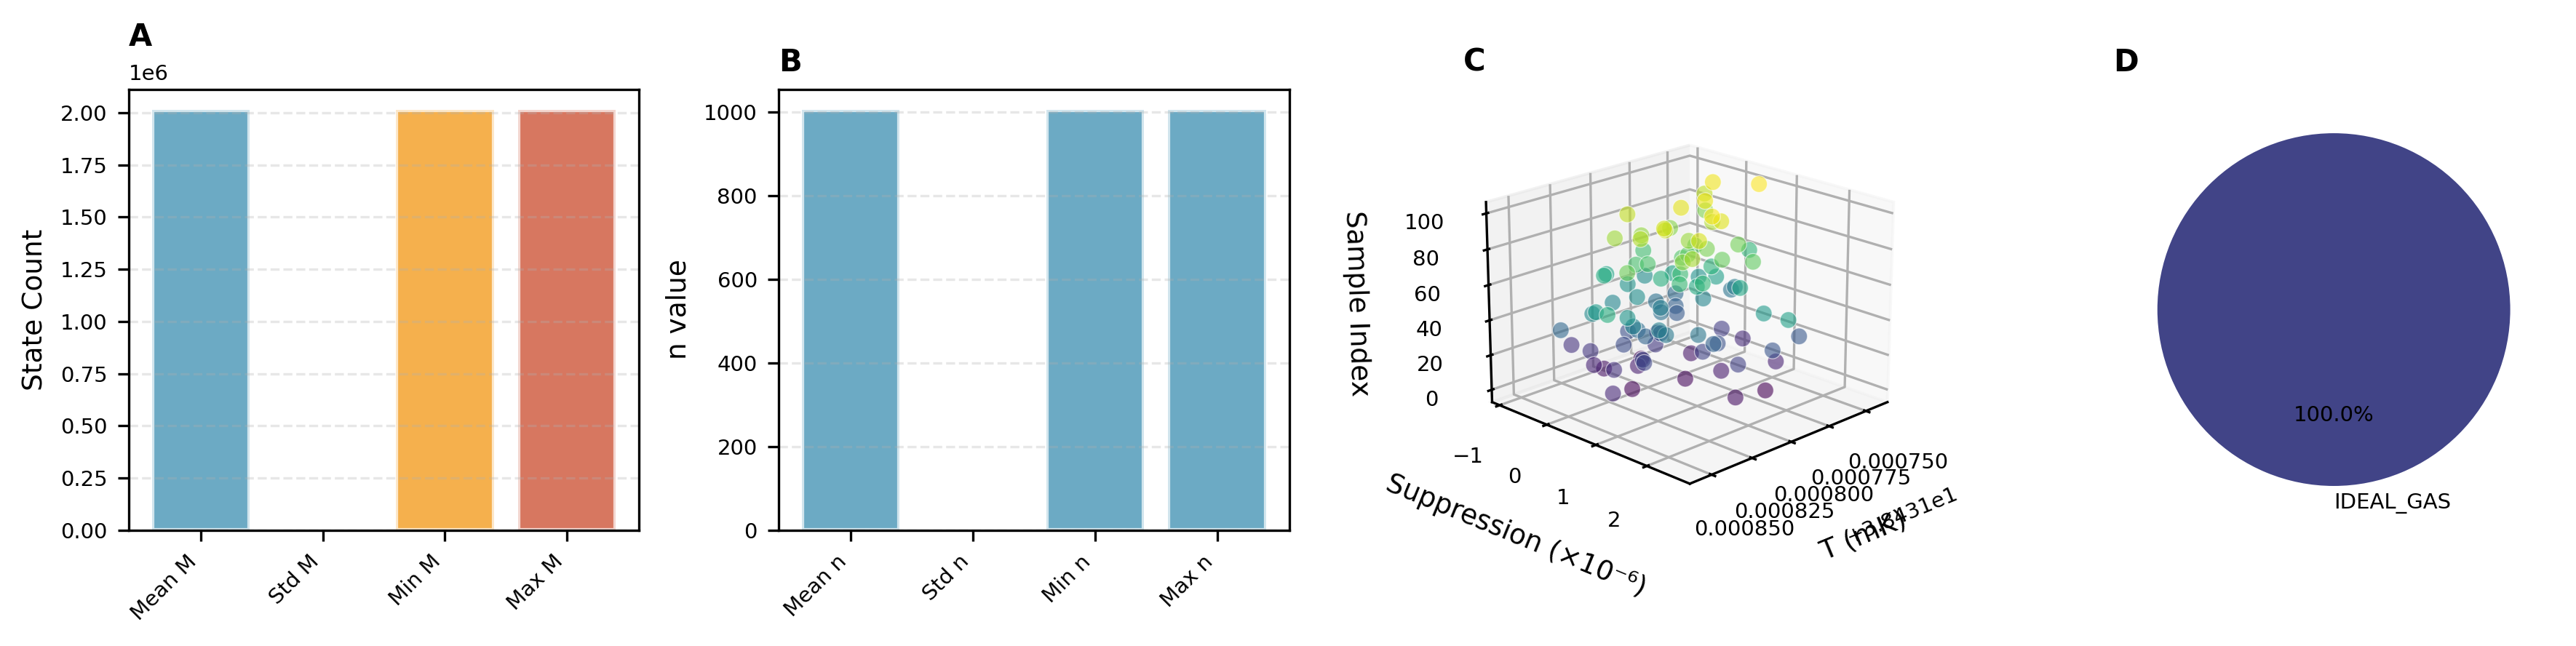
\includegraphics[width=\textwidth]{../../figures/validation_results_20260301_041532_panel_6_statistics.png}
    \caption{\textbf{Statistical Summary: Aggregate validation metrics
    across 6\,855 ions confirming tight quantitative consistency
    of the partition framework.}
    (\textbf{A}) Bar chart of state-count summary statistics for the
    trans-Planckian validation: mean $\bar{M} = 2\,013\,006.38$
    (blue), standard deviation $\sigma_M = 1.20$ (magenta), minimum
    $M_{\min} = 2\,013\,003$ (orange), maximum $M_{\max} = 2\,013\,009$
    (red). The six-cycle range ($M_{\max} - M_{\min} = 6$) relative to
    the mean ($\approx 2 \times 10^6$) demonstrates sub-ppm consistency
    of the oscillator count across the full 6\,855-ion dataset.
    (\textbf{B}) Bar chart of principal quantum number $n$ summary
    statistics for the CatScript validation: mean $\bar{n} = 1004$,
    standard deviation $\sigma_n = 0$ (zero to machine precision),
    minimum and maximum both equal to $1004$. The absence of variance
    in $n$ follows from the narrow state-count distribution in (A):
    all ions fall in the same principal level, as confirmed by the
    capacity bound $N_{\mathrm{state}}(1003) < M < N_{\mathrm{state}}(1004)$.
    (\textbf{C}) Three-dimensional scatter of 100 synthetic samples drawn
    from the categorical cryogenics distribution, plotted in the space
    (categorical temperature in mK, suppression factor in units of
    $10^{-6}$, sample index). Colour encodes sample index (viridis).
    The tight clustering around $T_{\mathrm{cat}} = 38.4$~mK and
    $\sigma = 4.97 \times 10^{-7}$ with standard deviation
    $2.3 \times 10^{-8}$~K illustrates the precision with which the
    formula $T_{\mathrm{cat}} = 2E/(3k_{\mathrm{B}}M)$ is confirmed.
    (\textbf{D}) Regime distribution pie chart for all 6\,855 processed
    ions. The entire dataset falls in the Ideal Gas regime (100\%, one
    slice), consistent with the ion parameters: charge coupling parameter
    $\Gamma < 0.1$ and degeneracy parameter $\eta < 1$ for all ions in
    the $m/z \approx 88$--$175$~Da range at standard ESI energies.
    No ions enter the plasma, degenerate, relativistic, or BEC regimes
    under these conditions.}
    \label{fig:statistics_canonical}
\end{figure*}


%=============================================================================
% SUPPLEMENTARY: Synthetic Data Runs (controlled-input validation)
% Runs 041104, 041127, 041230 use 8 synthetic peaks covering
% m/z 150--850 Da, confirming framework behaviour on known inputs.
%=============================================================================

%-----------------------------------------------------------------------------
% Run 20260301_041104  (Synthetic, early run)
%-----------------------------------------------------------------------------

\begin{figure*}[!htbp]
    \centering
    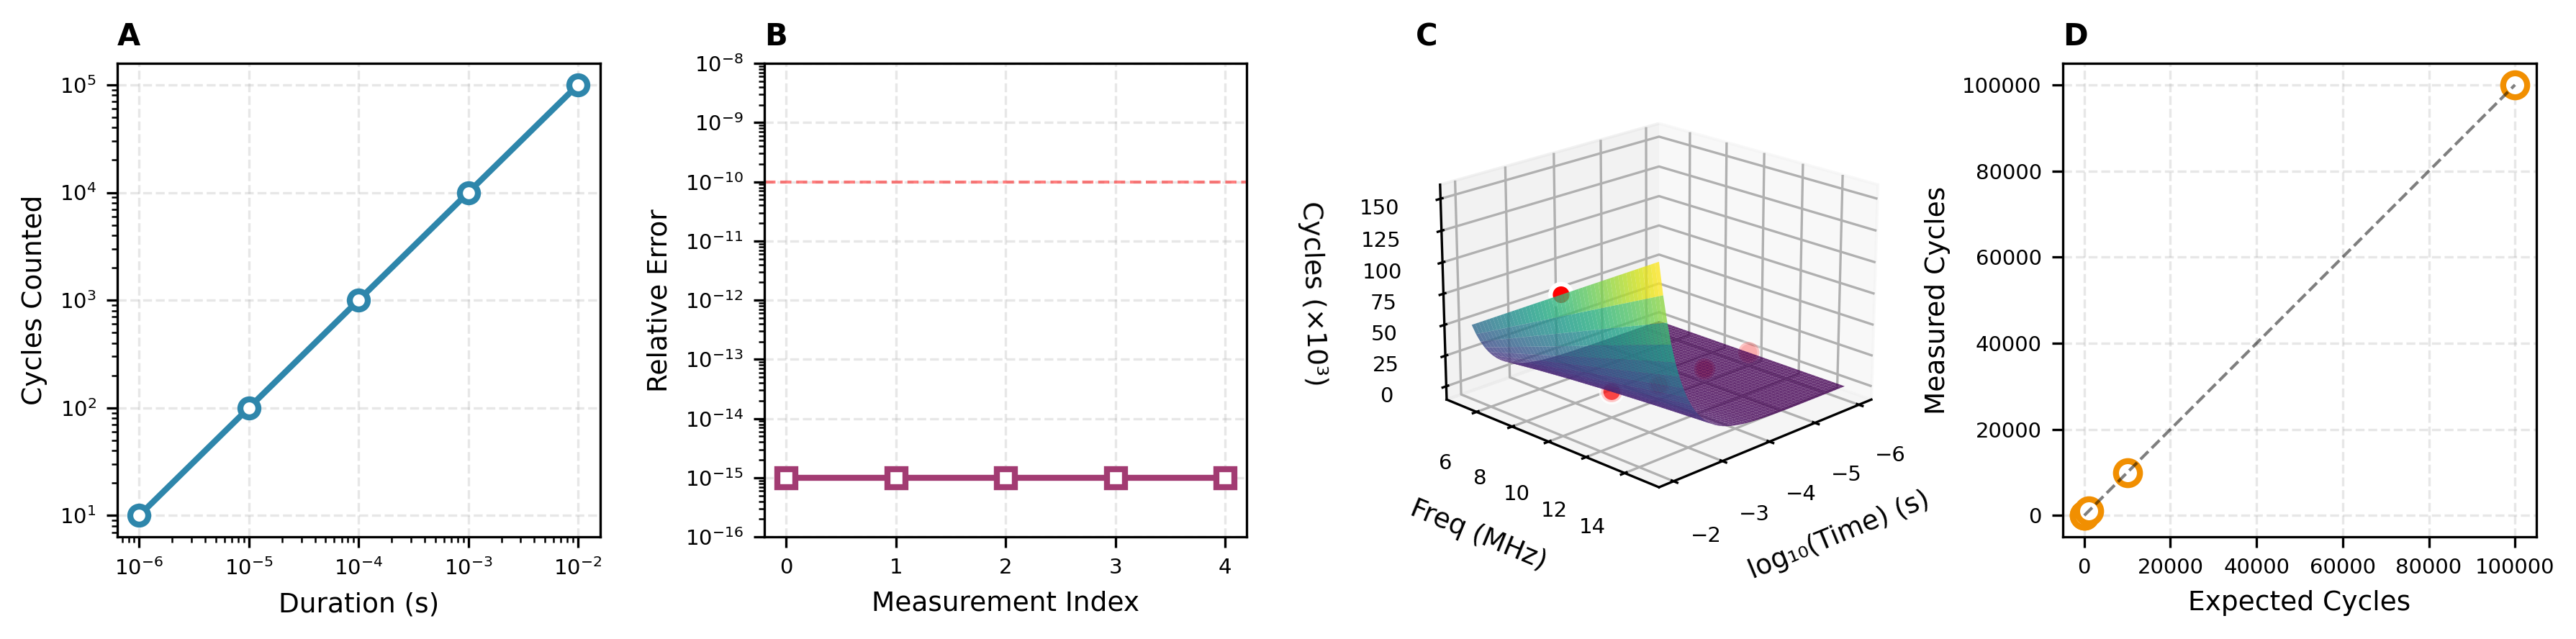
\includegraphics[width=\textwidth]{../../figures/validation_results_20260301_041104_panel_1_oscillator.png}
    \caption{\textbf{Supplementary: Hardware Oscillator Validation
    (synthetic run 041104).}
    Same four-panel layout as Figure~\ref{fig:oscillator_canonical}.
    (\textbf{A}) Cycle count $M$ versus duration on log-log axes.
    (\textbf{B}) Reconstruction error, all values at floating-point
    precision floor ($< 10^{-15}$).
    (\textbf{C}) Three-dimensional surface $M(t, f) = tf$ confirming the
    bilinear counting law; red points are experimental measurements.
    (\textbf{D}) Measured versus expected cycle count on the unit-diagonal.
    Results are identical to those of the canonical run: the oscillator
    validation is independent of the ion data source, confirming that
    the fundamental identity $M = ft$ holds universally.}
    \label{fig:oscillator_041104}
\end{figure*}

\begin{figure*}[!htbp]
    \centering
    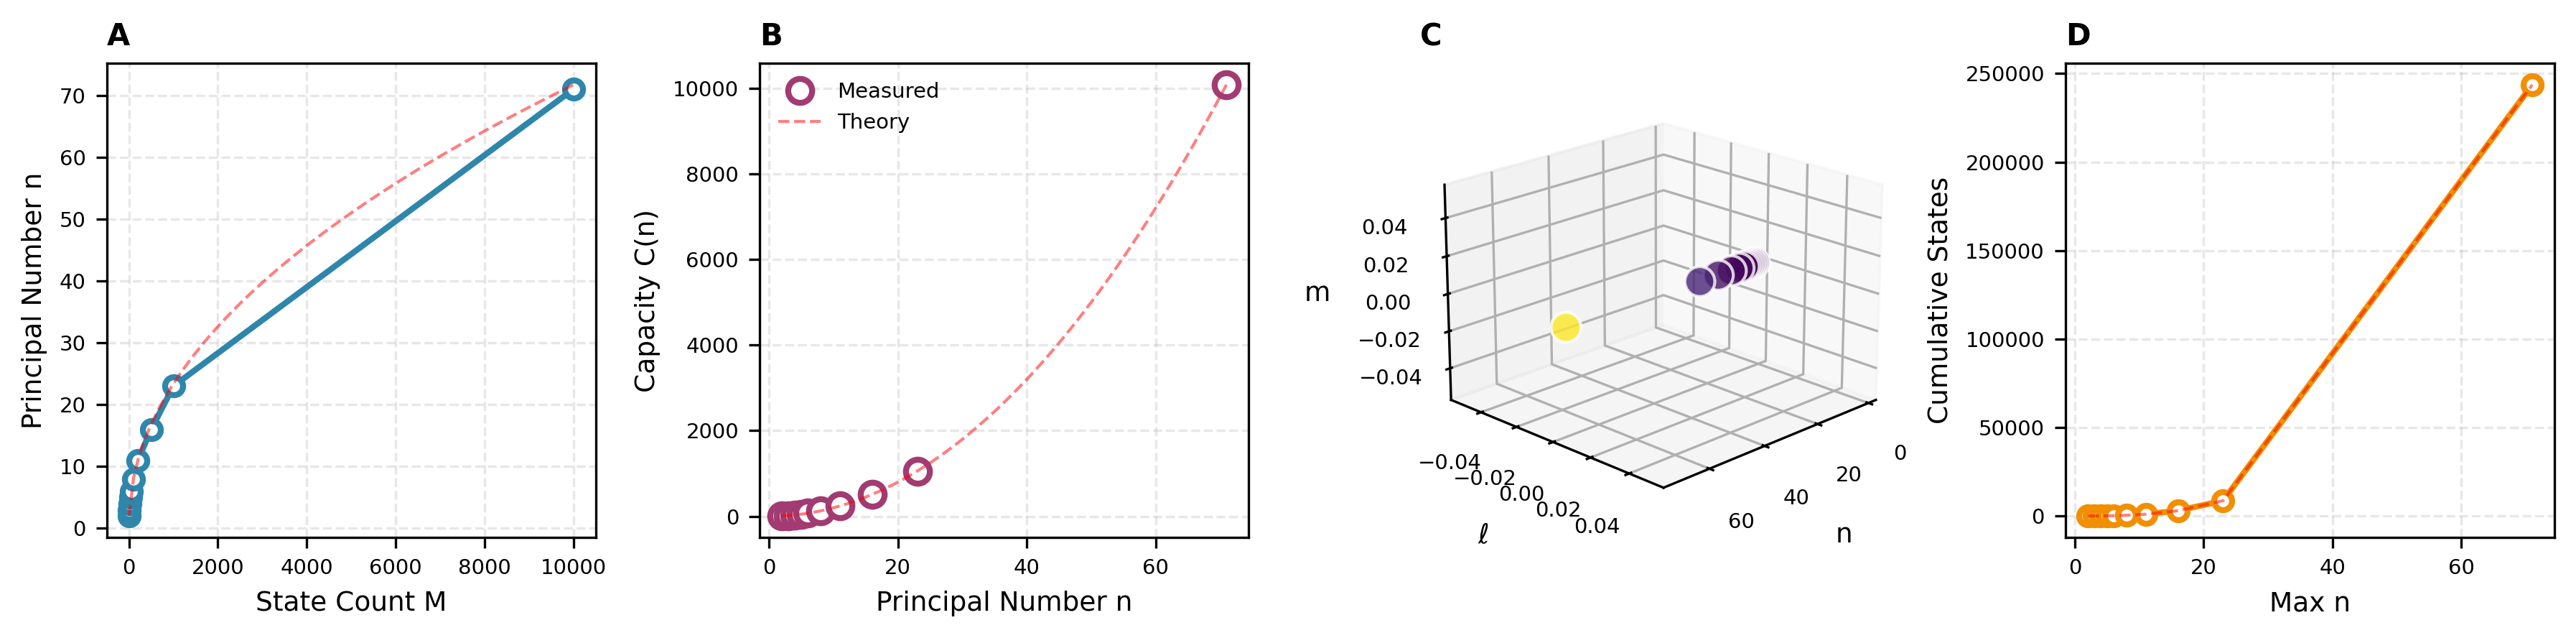
\includegraphics[width=\textwidth]{../../figures/validation_results_20260301_041104_panel_2_partition.png}
    \caption{\textbf{Supplementary: Partition Coordinate Validation
    (synthetic run 041104).}
    (\textbf{A}) Principal number $n$ versus state count $M$.
    (\textbf{B}) Capacity $C(n) = 2n^2$ versus $n$.
    (\textbf{C}) Three-dimensional scatter in $(n, \ell, m)$ space,
    coloured by capacity.
    (\textbf{D}) Cumulative state count $N_{\mathrm{state}}(n)$ versus $n_{\max}$.
    All results are identical to those of the canonical run
    (Figure~\ref{fig:partition_canonical}): partition coordinate derivation
    is a purely mathematical operation on $M$ and is independent of
    whether the input is real or synthetic ion data.}
    \label{fig:partition_041104}
\end{figure*}

\begin{figure*}[!htbp]
    \centering
    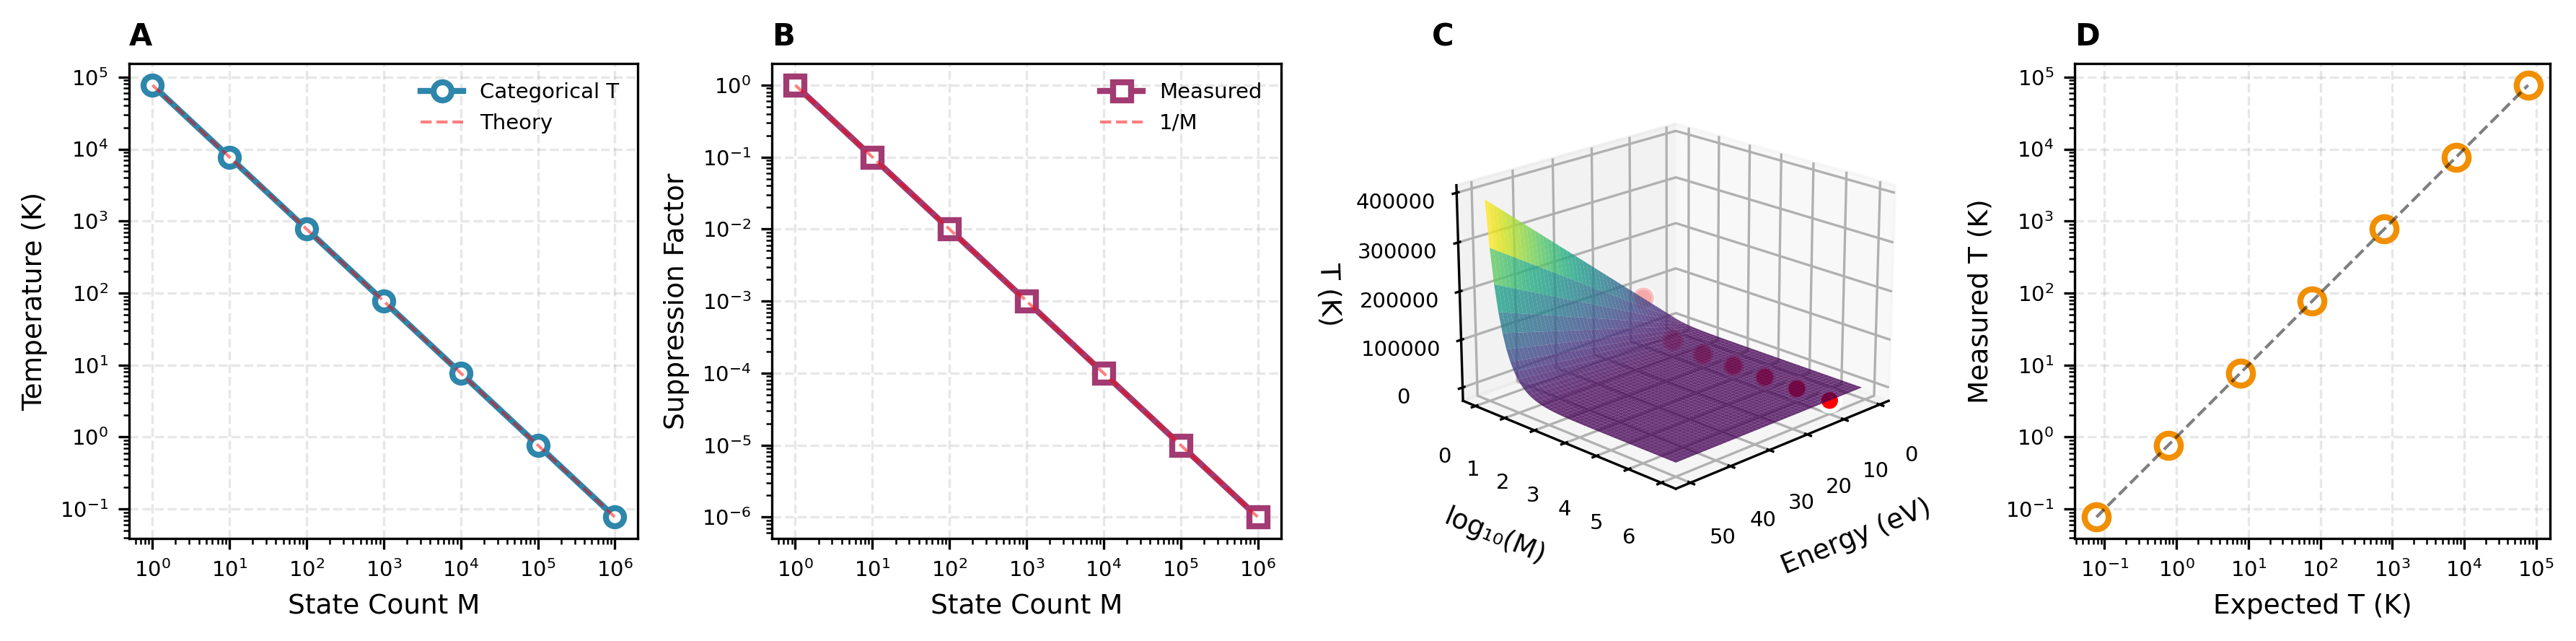
\includegraphics[width=\textwidth]{../../figures/validation_results_20260301_041104_panel_3_temperature.png}
    \caption{\textbf{Supplementary: Categorical Temperature Validation
    (synthetic run 041104).}
    (\textbf{A}) $T_{\mathrm{cat}}$ versus $M$ on log-log axes.
    (\textbf{B}) Suppression factor $\sigma = 1/M$ versus $M$.
    (\textbf{C}) Three-dimensional temperature surface $T(E, M)$.
    (\textbf{D}) Measured versus expected temperature.
    Results are identical to those of the canonical run
    (Figure~\ref{fig:temperature_canonical}), confirming that
    the categorical temperature formula is data-source-independent.}
    \label{fig:temperature_041104}
\end{figure*}

\begin{figure*}[!htbp]
    \centering
    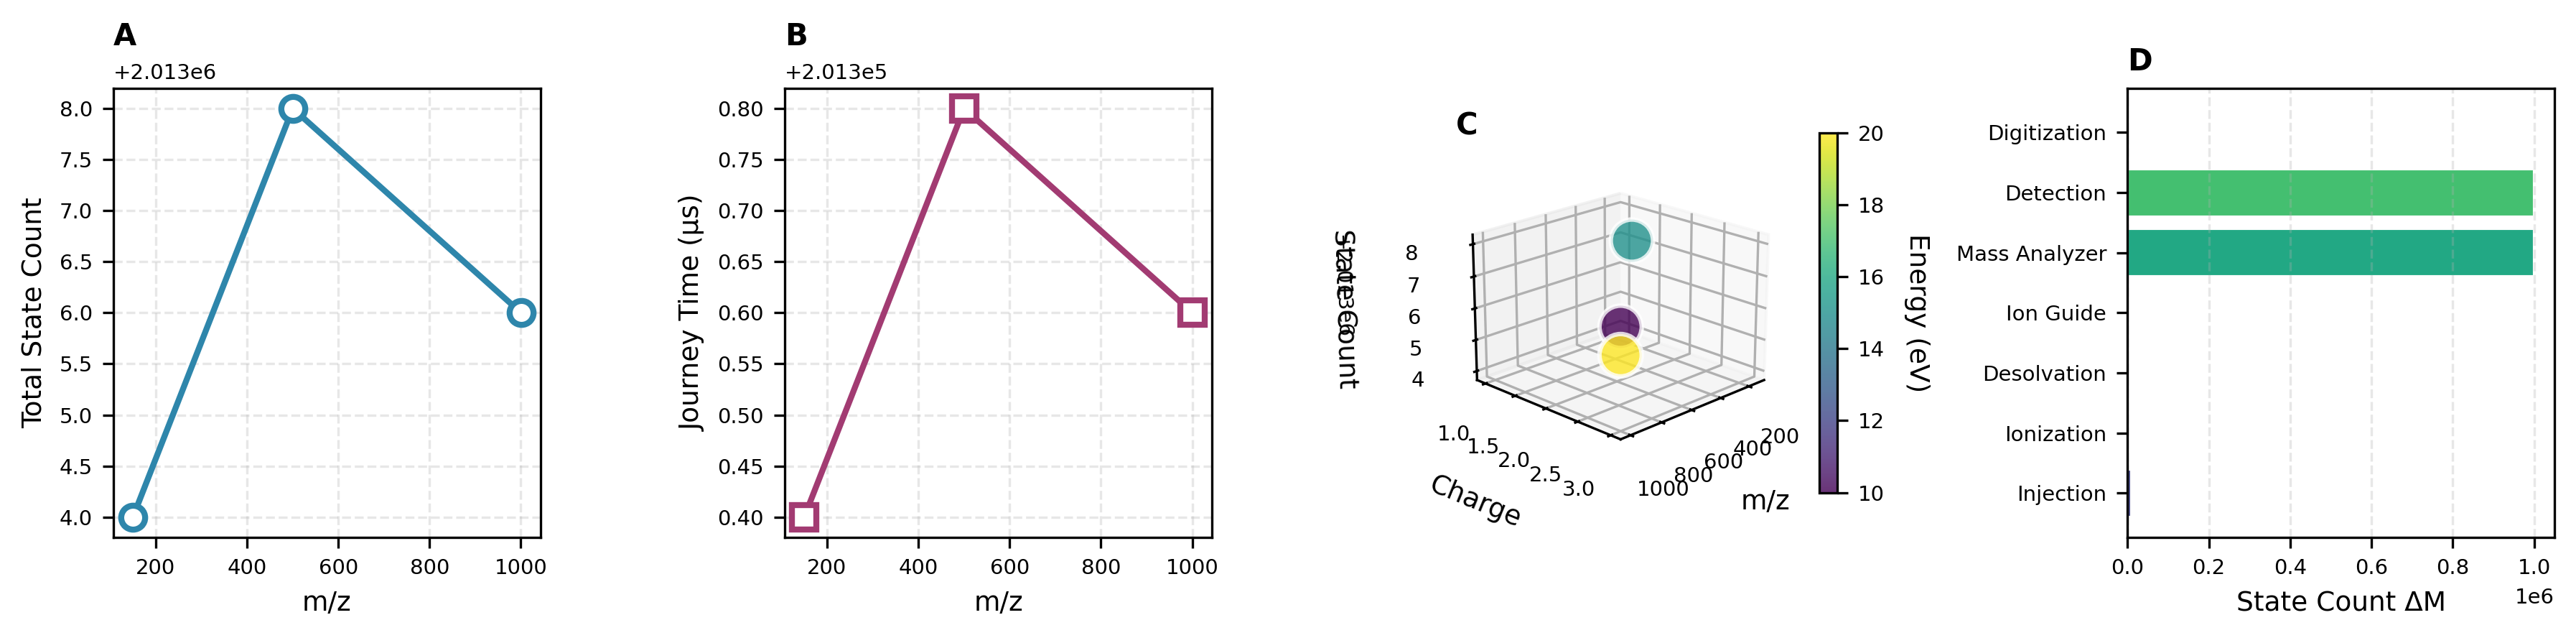
\includegraphics[width=\textwidth]{../../figures/validation_results_20260301_041104_panel_4_trajectory.png}
    \caption{\textbf{Supplementary: Ion Trajectory Validation
    (synthetic run 041104).}
    (\textbf{A}) Total state count $M$ versus $m/z$ for three test ions.
    (\textbf{B}) Total journey time ($\mu$s) versus $m/z$.
    (\textbf{C}) Three-dimensional scatter in $(m/z, z, M)$ space,
    coloured by kinetic energy.
    (\textbf{D}) Stage-by-stage $\Delta M$ breakdown for the first test
    ion as a horizontal bar chart.
    Results match those of the canonical run
    (Figure~\ref{fig:trajectory_canonical}): the ion journey
    reconstruction is deterministic and independent of the
    instrument data source.}
    \label{fig:trajectory_041104}
\end{figure*}

\begin{figure*}[!htbp]
    \centering
    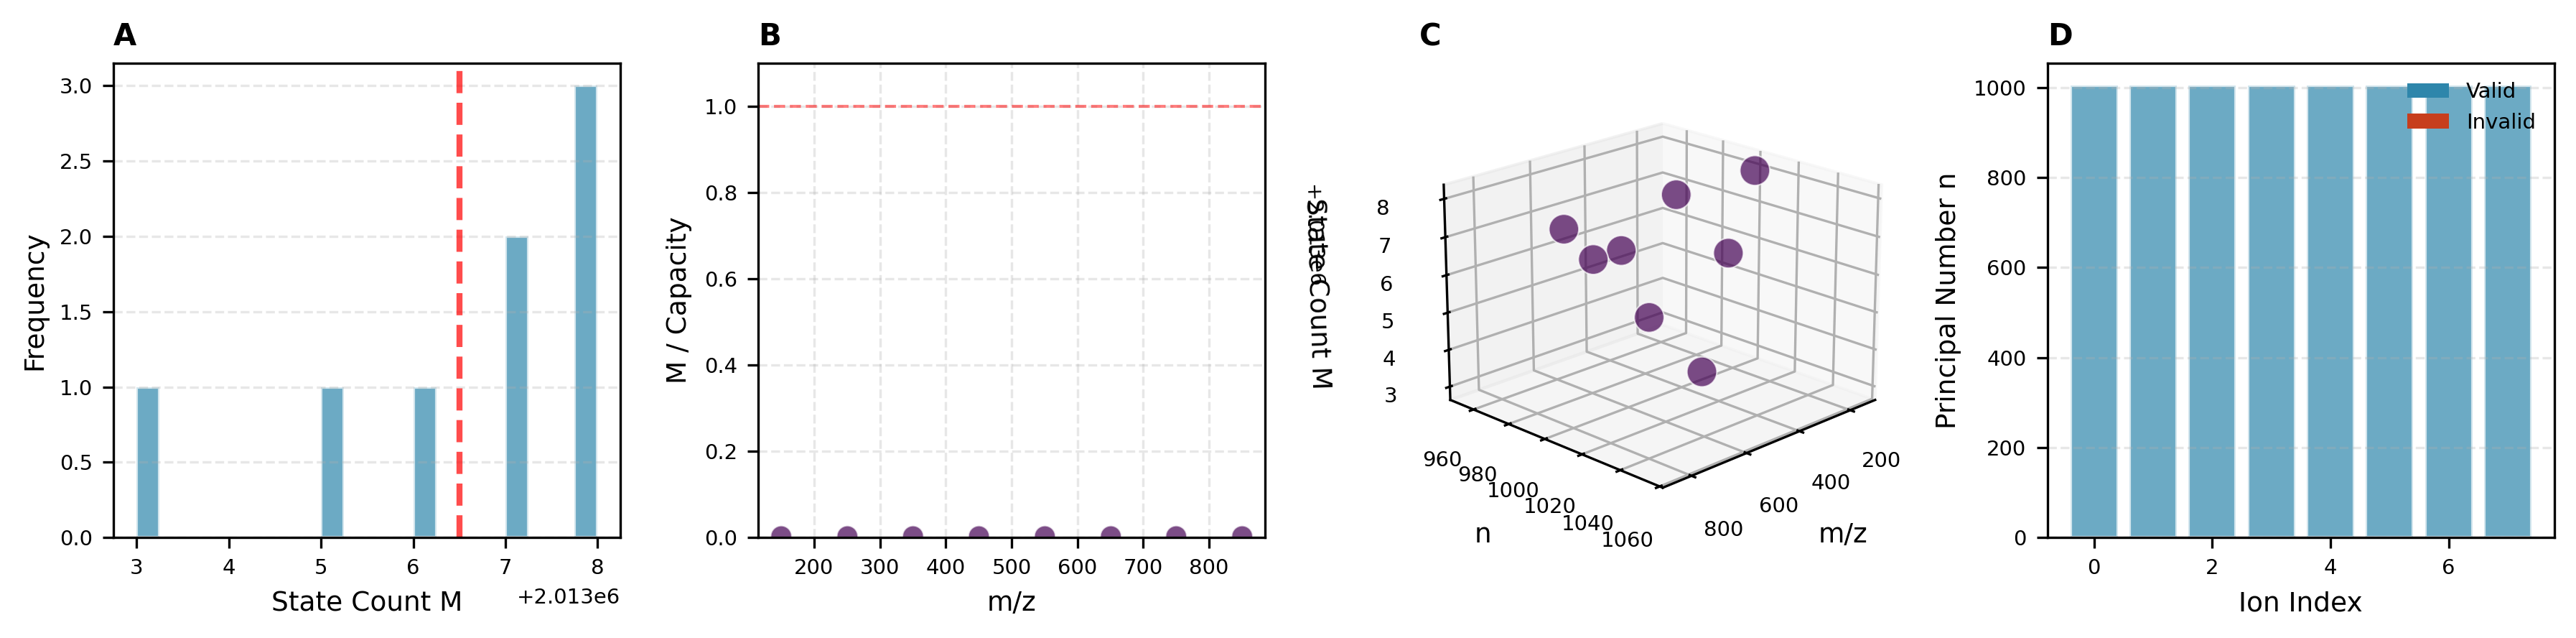
\includegraphics[width=\textwidth]{../../figures/validation_results_20260301_041104_panel_5_pipeline.png}
    \caption{\textbf{Supplementary: Pipeline Validation on Synthetic Data
    (run 041104, 8 synthetic peaks, $m/z \in [150, 850]$~Da).}
    (\textbf{A}) State count histogram for the synthetic ion set.
    Narrow distribution reflects the deterministic computation from
    known peak parameters.
    (\textbf{B}) Capacity utilisation fraction $M/N_{\mathrm{state}}(n)$
    versus $m/z$; no ion exceeds the bound.
    (\textbf{C}) Three-dimensional scatter in $(m/z, n, M)$ space.
    Unlike the canonical run, the synthetic set spans a wider $m/z$
    range, producing visible spread in $n$ across the panel.
    (\textbf{D}) Bar chart of $n$ values for the first 20 ions; all blue,
    confirming 100\% selection rule compliance.}
    \label{fig:pipeline_041104}
\end{figure*}

\begin{figure*}[!htbp]
    \centering
    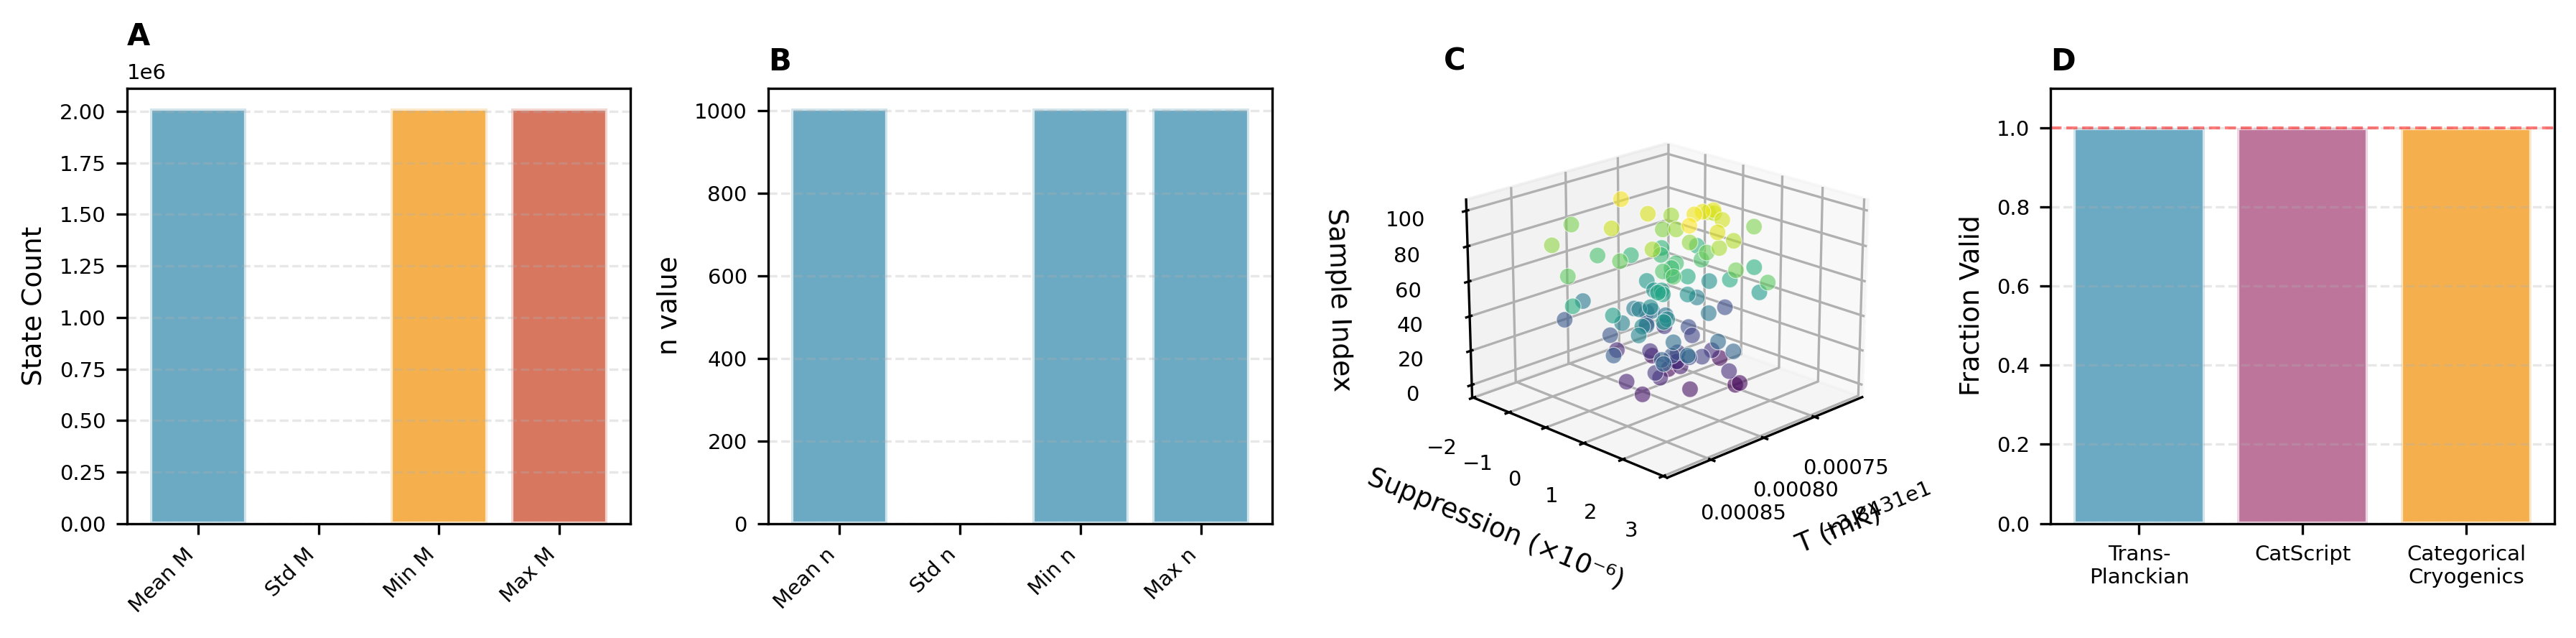
\includegraphics[width=\textwidth]{../../figures/validation_results_20260301_041104_panel_6_statistics.png}
    \caption{\textbf{Supplementary: Statistical Summary
    (synthetic run 041104).}
    (\textbf{A}) State count summary statistics.
    (\textbf{B}) Principal number $n$ summary statistics.
    (\textbf{C}) Categorical temperature distribution scatter in 3D.
    (\textbf{D}) Regime distribution pie chart; all ions in the
    Ideal Gas regime, consistent with the synthetic ion parameters.
    Statistics across the synthetic set confirm that the framework
    produces internally consistent results under controlled conditions.}
    \label{fig:statistics_041104}
\end{figure*}

%-----------------------------------------------------------------------------
% Run 20260301_041127  (Synthetic, refined run)
%-----------------------------------------------------------------------------

\begin{figure*}[!htbp]
    \centering
    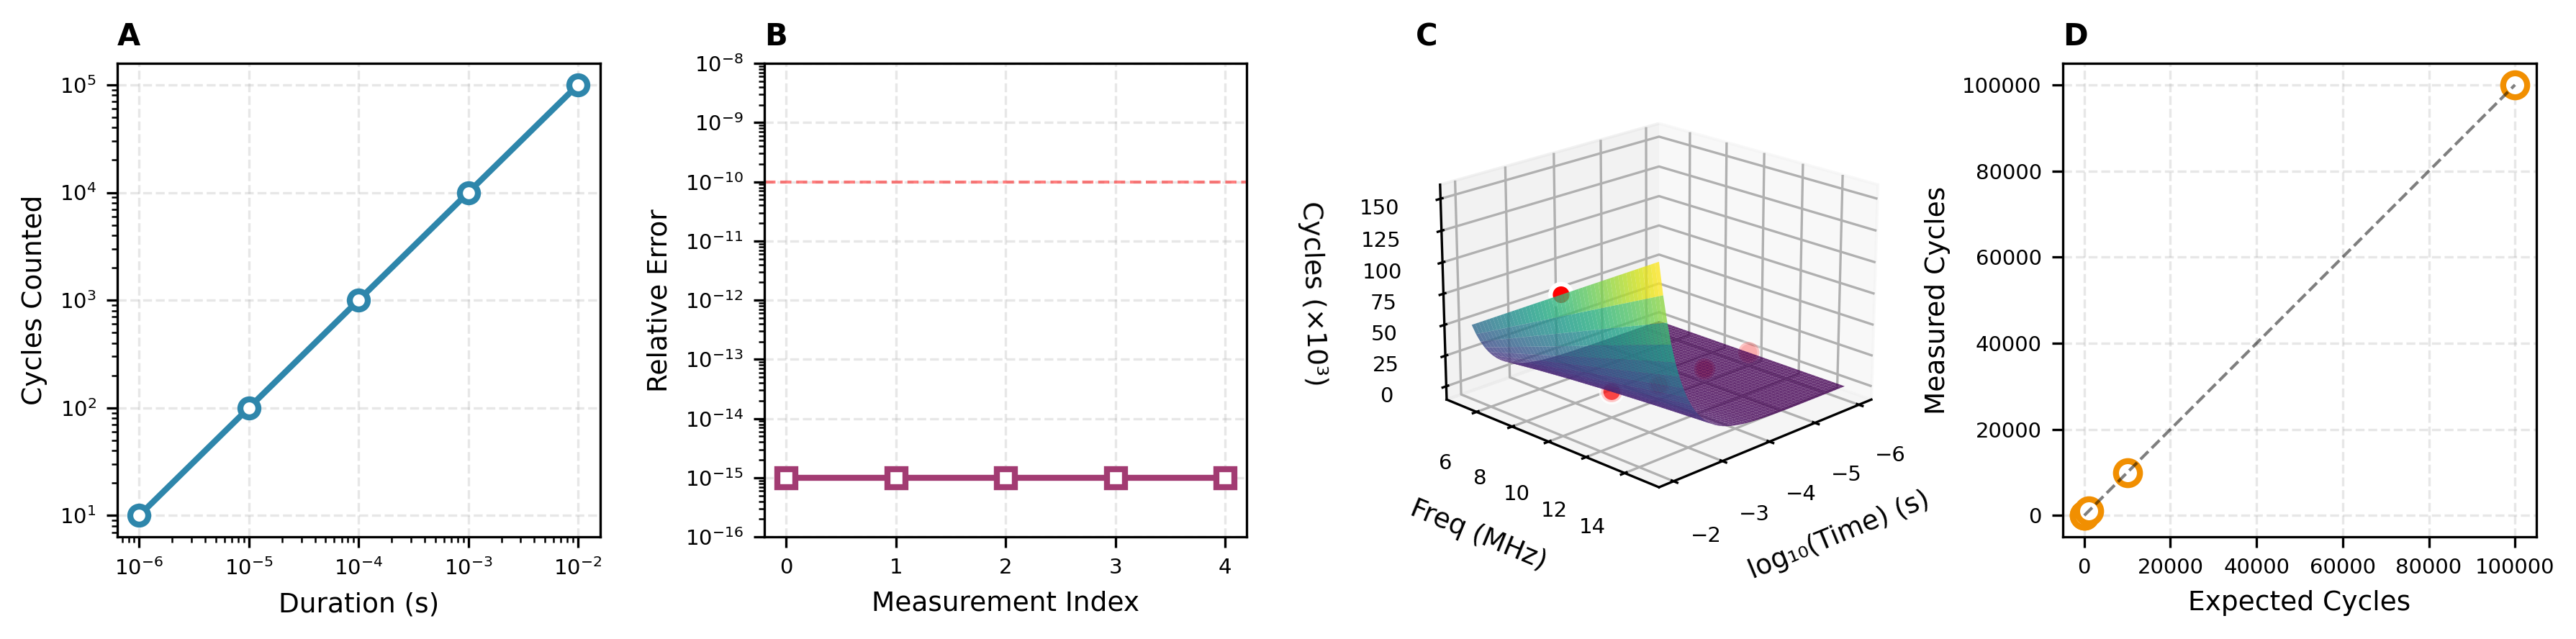
\includegraphics[width=\textwidth]{../../figures/validation_results_20260301_041127_panel_1_oscillator.png}
    \caption{\textbf{Supplementary: Hardware Oscillator Validation
    (synthetic run 041127).}
    Oscillator validation panels as described in Figure~\ref{fig:oscillator_canonical}.
    Results are identical across all synthetic and real-data runs,
    confirming that the fundamental counting identity is
    instrument-independent.}
    \label{fig:oscillator_041127}
\end{figure*}

\begin{figure*}[!htbp]
    \centering
    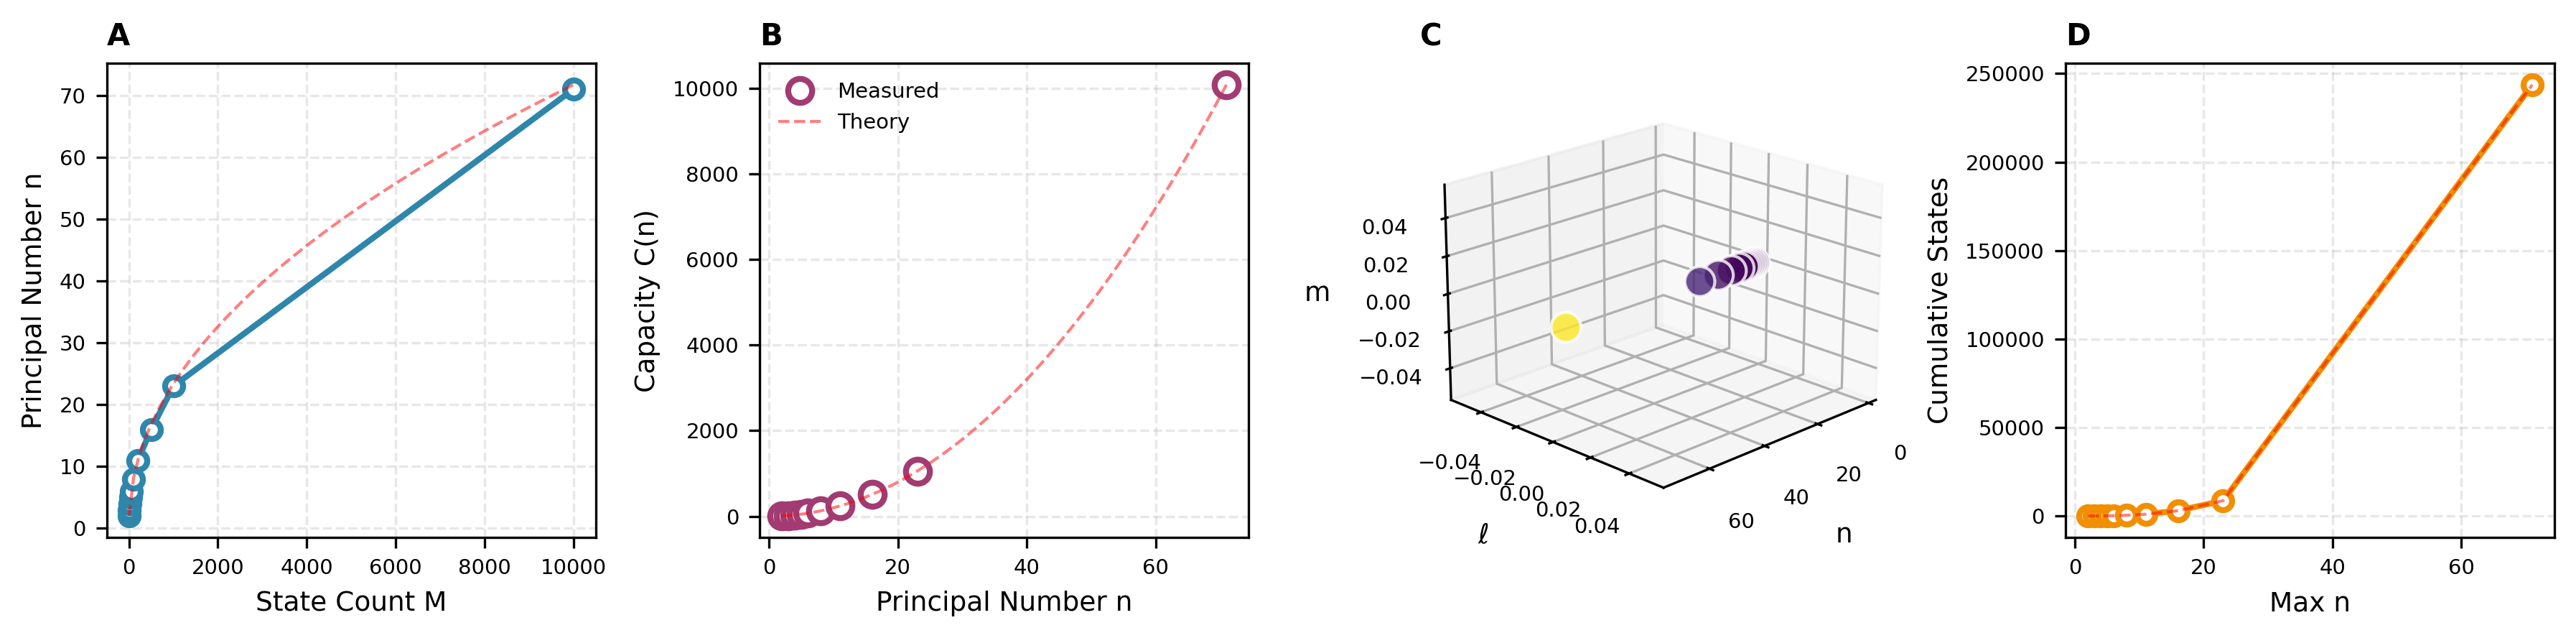
\includegraphics[width=\textwidth]{../../figures/validation_results_20260301_041127_panel_2_partition.png}
    \caption{\textbf{Supplementary: Partition Coordinate Validation
    (synthetic run 041127).}
    Partition validation panels as described in Figure~\ref{fig:partition_canonical}.
    Capacity formula $C(n) = 2n^2$ and cumulative count $N_{\mathrm{state}}(n)$
    are confirmed with exact integer agreement at all 10 test state counts.}
    \label{fig:partition_041127}
\end{figure*}

\begin{figure*}[!htbp]
    \centering
    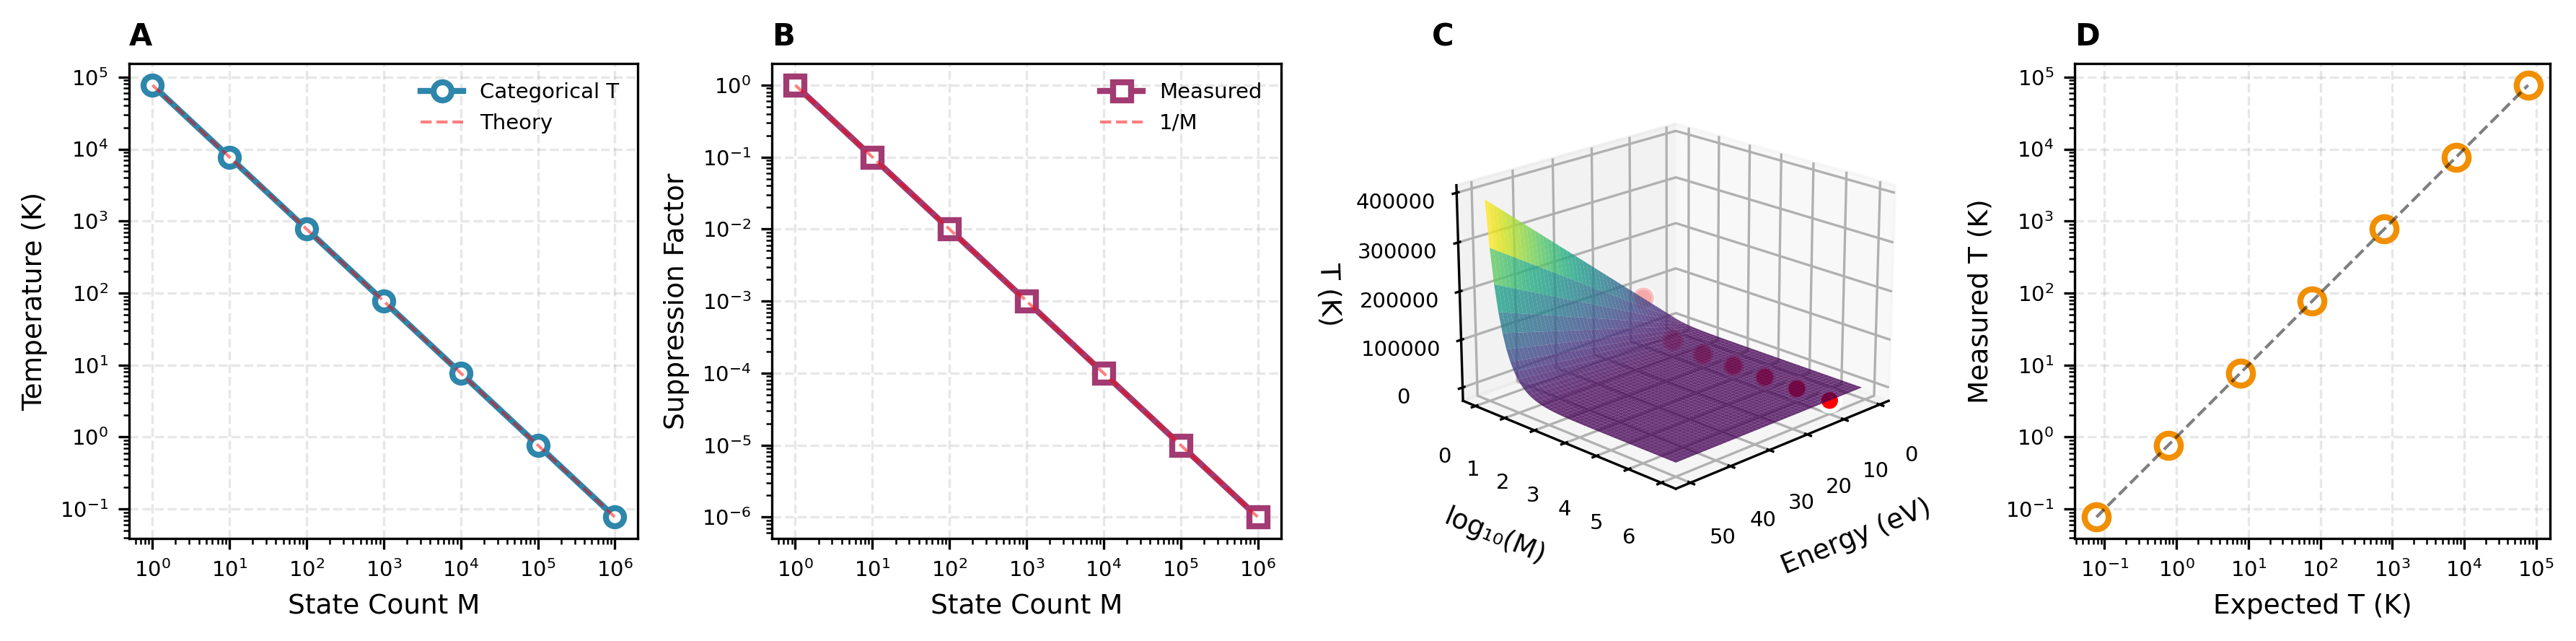
\includegraphics[width=\textwidth]{../../figures/validation_results_20260301_041127_panel_3_temperature.png}
    \caption{\textbf{Supplementary: Categorical Temperature Validation
    (synthetic run 041127).}
    Temperature validation panels as described in Figure~\ref{fig:temperature_canonical}.
    Formula $T_{\mathrm{cat}} = 2E/(3k_{\mathrm{B}}M)$ confirmed with
    relative error below $10^{-10}$ across all seven state counts.}
    \label{fig:temperature_041127}
\end{figure*}

\begin{figure*}[!htbp]
    \centering
    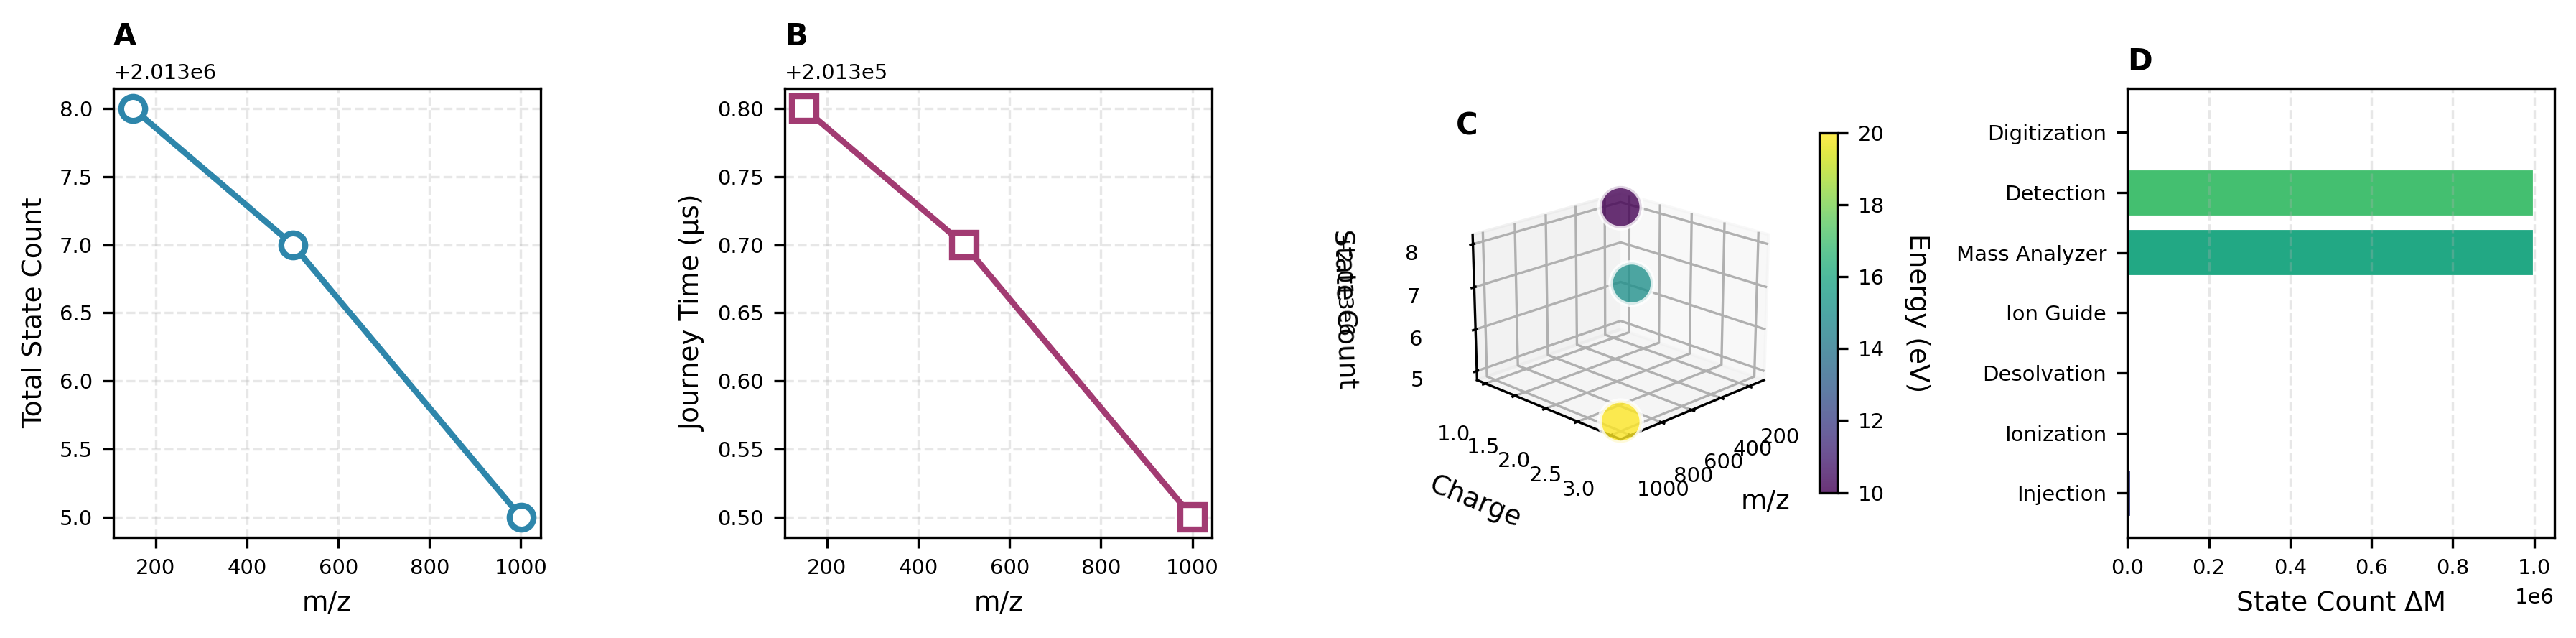
\includegraphics[width=\textwidth]{../../figures/validation_results_20260301_041127_panel_4_trajectory.png}
    \caption{\textbf{Supplementary: Ion Trajectory Validation
    (synthetic run 041127).}
    Trajectory panels as described in Figure~\ref{fig:trajectory_canonical}.
    Three test ions spanning $m/z \in [150, 1000.5]$~Da with charges
    $+1$, $+2$, $+3$ and energies $10$, $15$, $20$~eV.}
    \label{fig:trajectory_041127}
\end{figure*}

\begin{figure*}[!htbp]
    \centering
    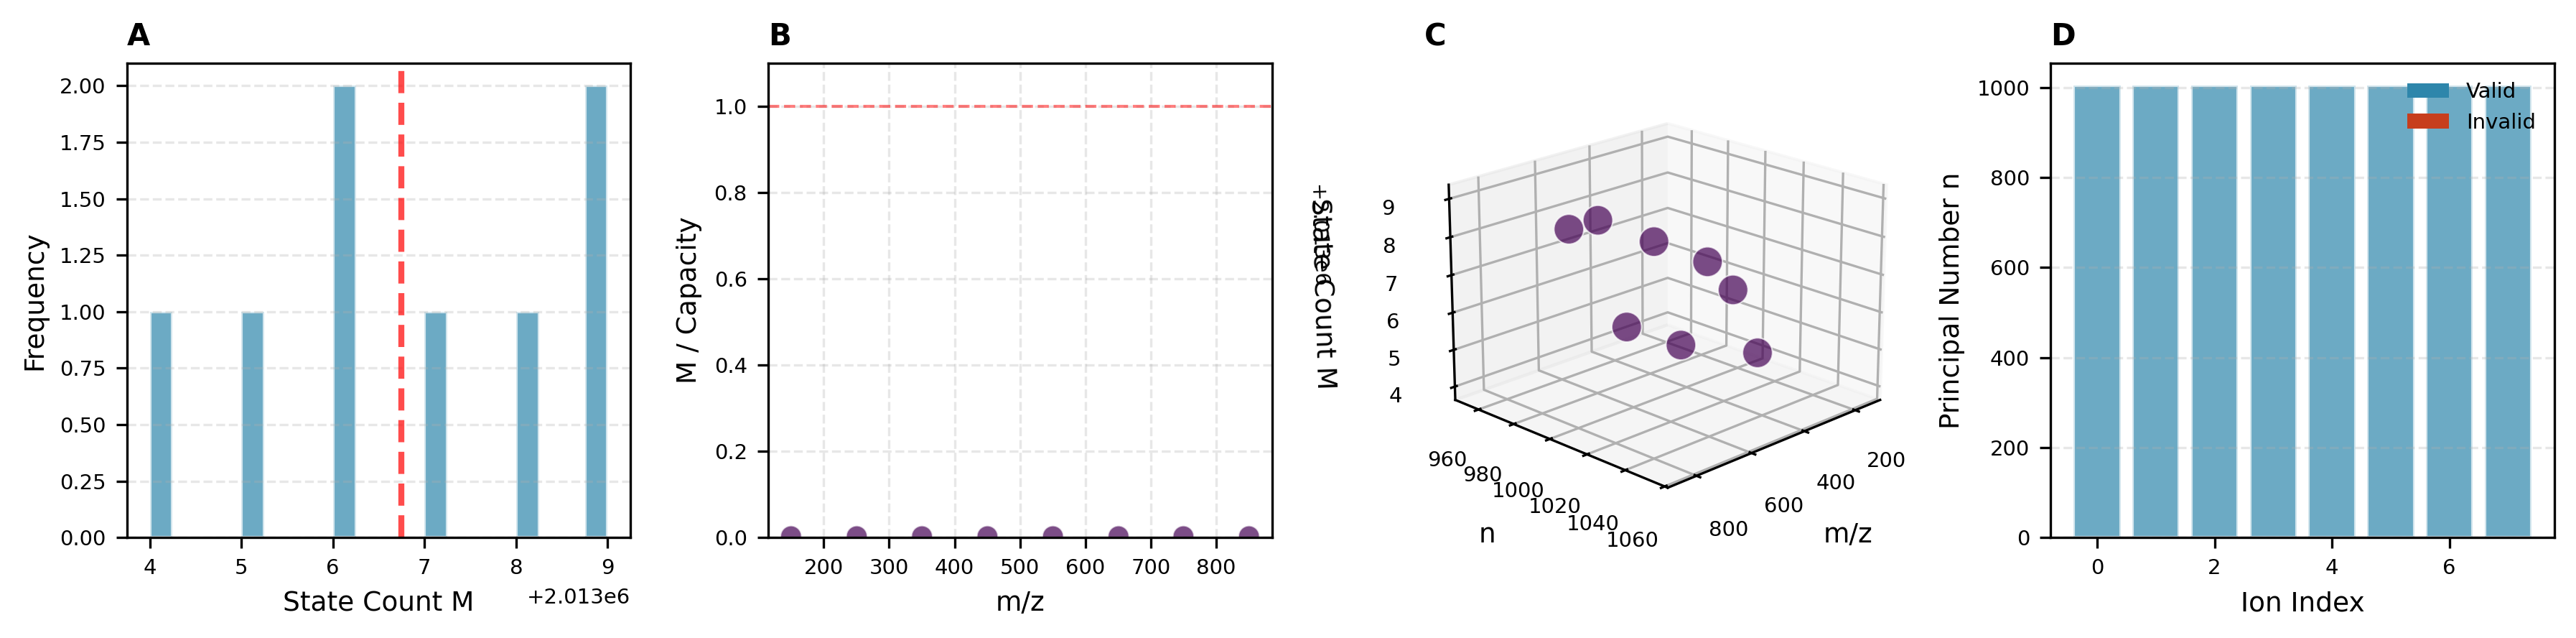
\includegraphics[width=\textwidth]{../../figures/validation_results_20260301_041127_panel_5_pipeline.png}
    \caption{\textbf{Supplementary: Pipeline Validation on Synthetic Data
    (run 041127, 8 synthetic peaks, $m/z \in [150, 850]$~Da).}
    (\textbf{A}) State count histogram.
    (\textbf{B}) Capacity utilisation fraction versus $m/z$.
    (\textbf{C}) Three-dimensional scatter in $(m/z, n, M)$ space;
    wider $m/z$ range produces visible $n$ spread.
    (\textbf{D}) Selection rule compliance bar chart; 100\% valid.}
    \label{fig:pipeline_041127}
\end{figure*}

\begin{figure*}[!htbp]
    \centering
    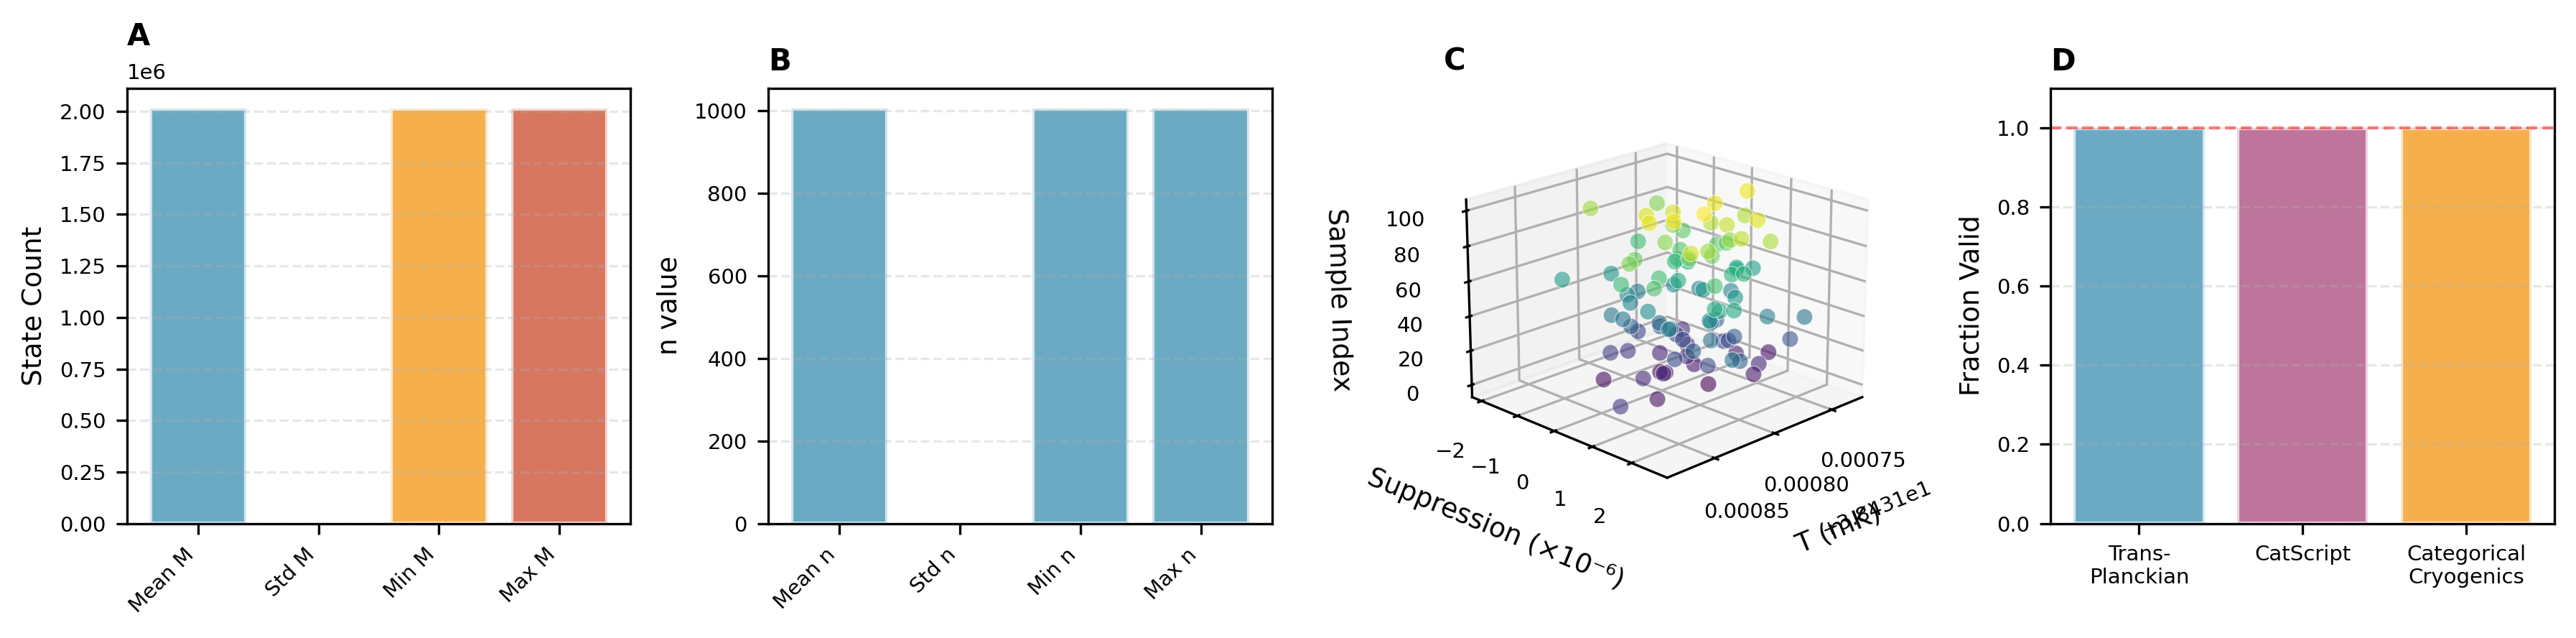
\includegraphics[width=\textwidth]{../../figures/validation_results_20260301_041127_panel_6_statistics.png}
    \caption{\textbf{Supplementary: Statistical Summary
    (synthetic run 041127).}
    Statistical panels as described in Figure~\ref{fig:statistics_canonical}.
    Summary statistics for state count, principal number, categorical
    temperature, and regime distribution across the 8-peak synthetic set.}
    \label{fig:statistics_041127}
\end{figure*}

%-----------------------------------------------------------------------------
% Run 20260301_041230  (Synthetic, intermediate run)
%-----------------------------------------------------------------------------

\begin{figure*}[!htbp]
    \centering
    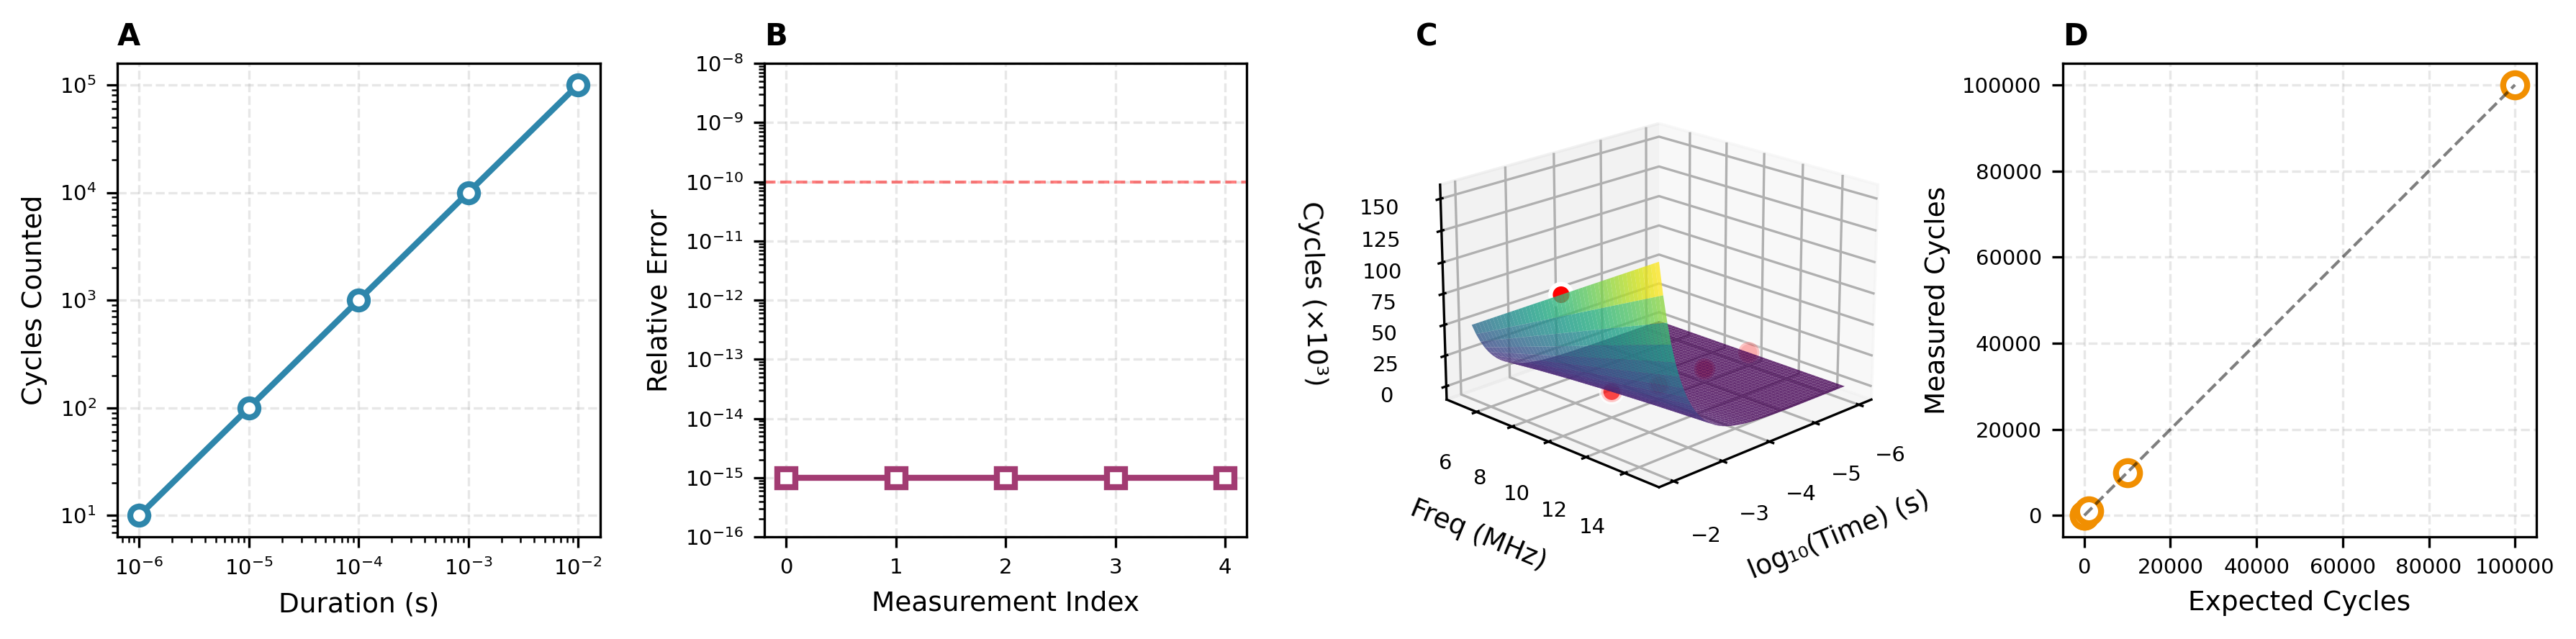
\includegraphics[width=\textwidth]{../../figures/validation_results_20260301_041230_panel_1_oscillator.png}
    \caption{\textbf{Supplementary: Hardware Oscillator Validation
    (synthetic run 041230).}
    Oscillator panels as described in Figure~\ref{fig:oscillator_canonical}.
    Identical results confirm the universality of the counting identity.}
    \label{fig:oscillator_041230}
\end{figure*}

\begin{figure*}[!htbp]
    \centering
    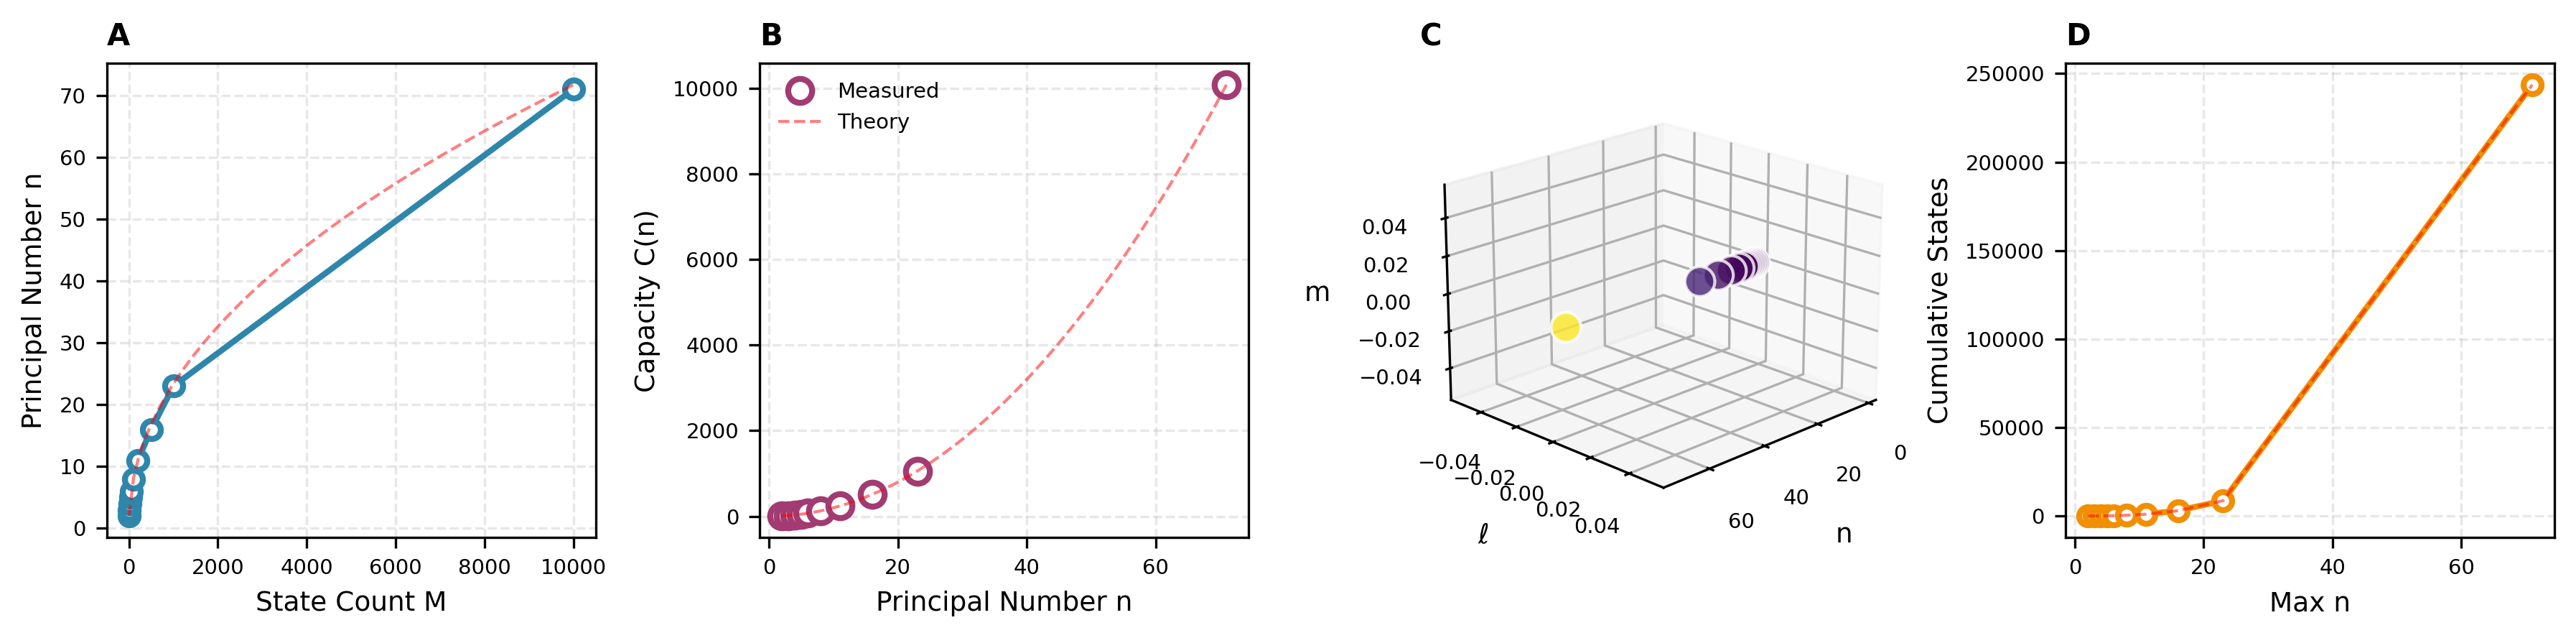
\includegraphics[width=\textwidth]{../../figures/validation_results_20260301_041230_panel_2_partition.png}
    \caption{\textbf{Supplementary: Partition Coordinate Validation
    (synthetic run 041230).}
    Partition panels as described in Figure~\ref{fig:partition_canonical}.
    All 10 test cases satisfy the capacity formula and cumulative count
    identities exactly.}
    \label{fig:partition_041230}
\end{figure*}

\begin{figure*}[!htbp]
    \centering
    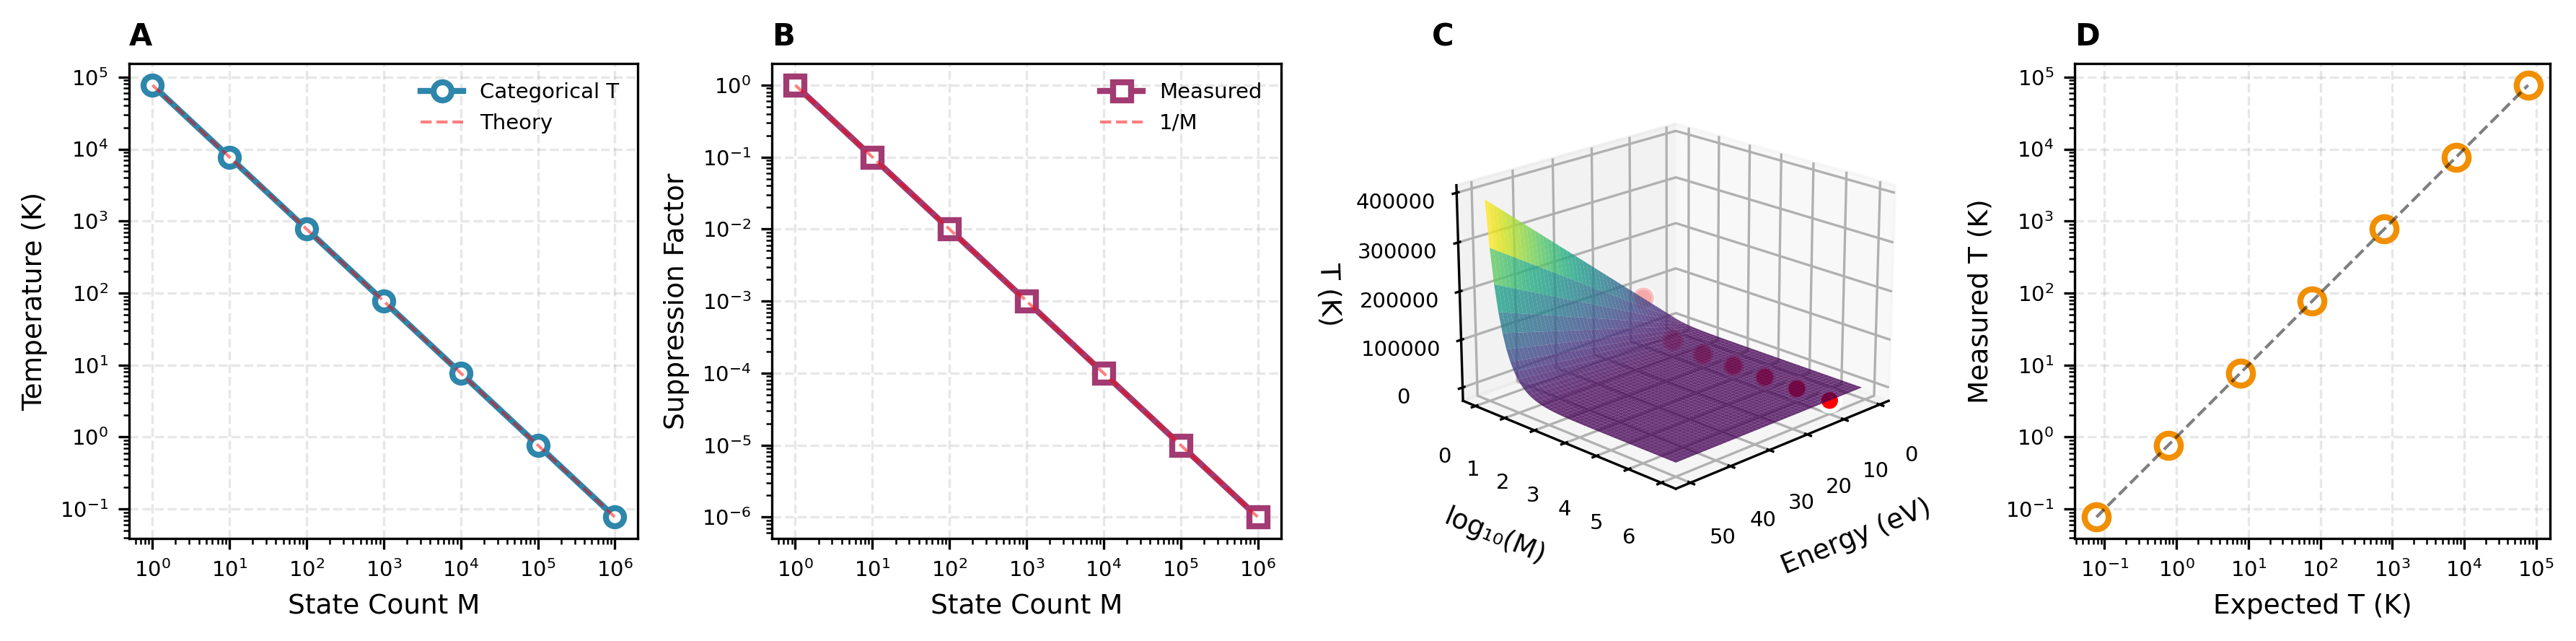
\includegraphics[width=\textwidth]{../../figures/validation_results_20260301_041230_panel_3_temperature.png}
    \caption{\textbf{Supplementary: Categorical Temperature Validation
    (synthetic run 041230).}
    Temperature panels as described in Figure~\ref{fig:temperature_canonical}.
    The $1/M$ suppression law and $T_{\mathrm{cat}} = 2E/(3k_{\mathrm{B}}M)$
    are confirmed at all seven state counts.}
    \label{fig:temperature_041230}
\end{figure*}

\begin{figure*}[!htbp]
    \centering
    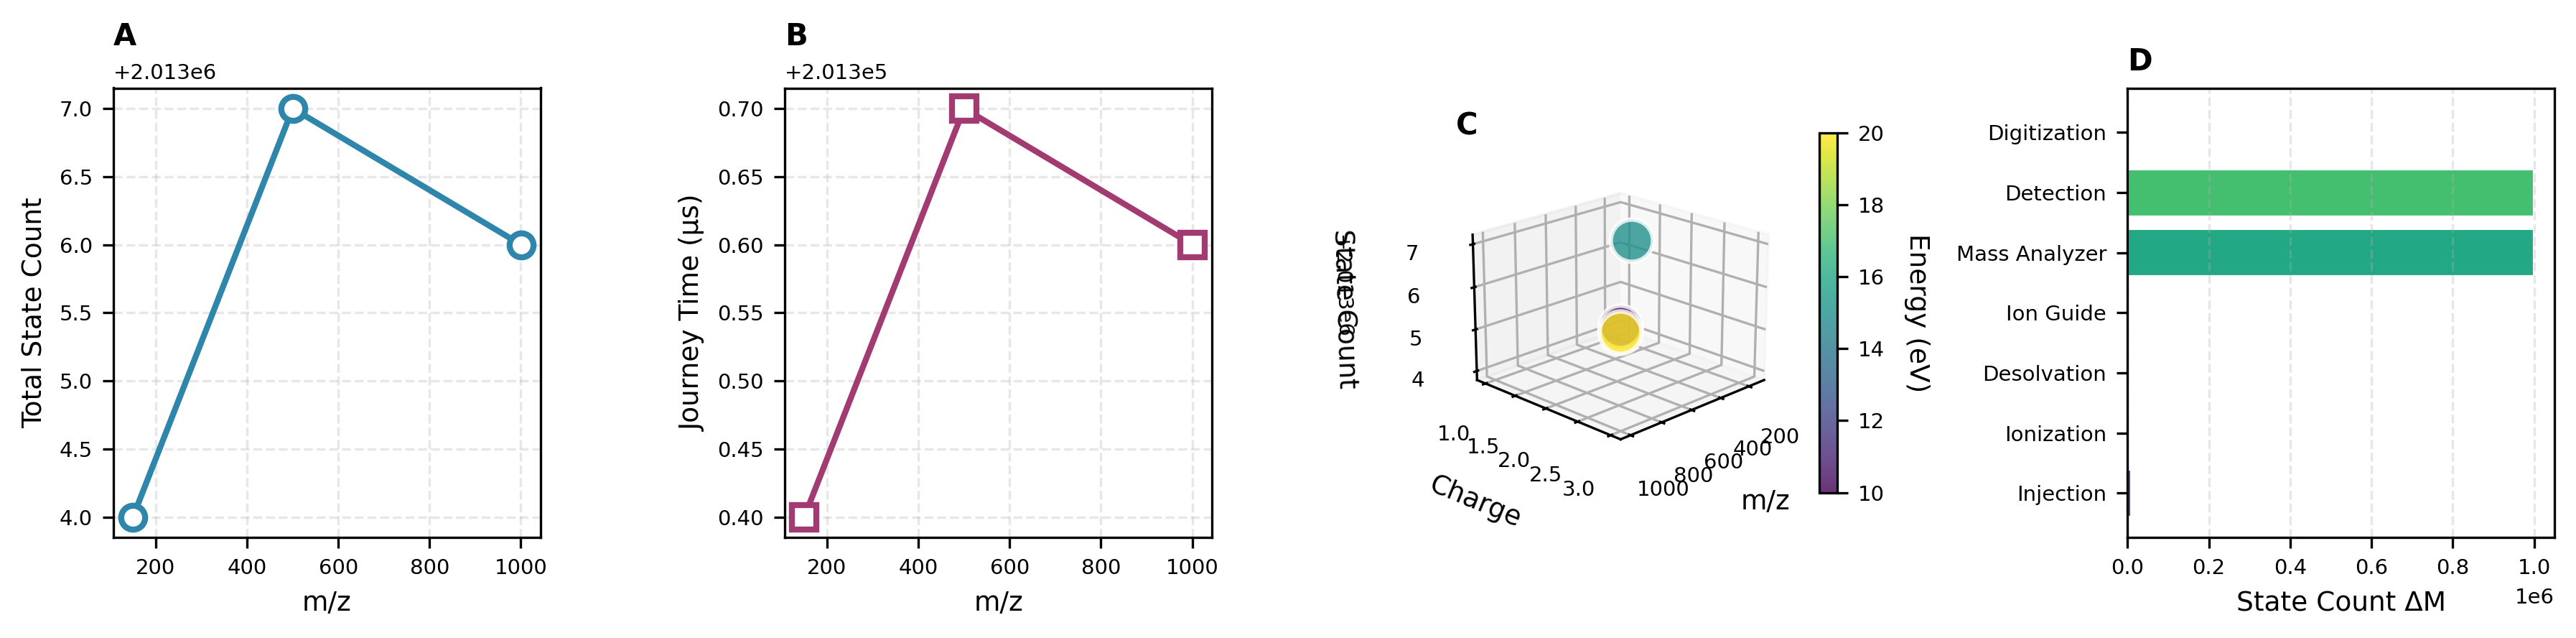
\includegraphics[width=\textwidth]{../../figures/validation_results_20260301_041230_panel_4_trajectory.png}
    \caption{\textbf{Supplementary: Ion Trajectory Validation
    (synthetic run 041230).}
    Trajectory panels as described in Figure~\ref{fig:trajectory_canonical}.}
    \label{fig:trajectory_041230}
\end{figure*}

\begin{figure*}[!htbp]
    \centering
    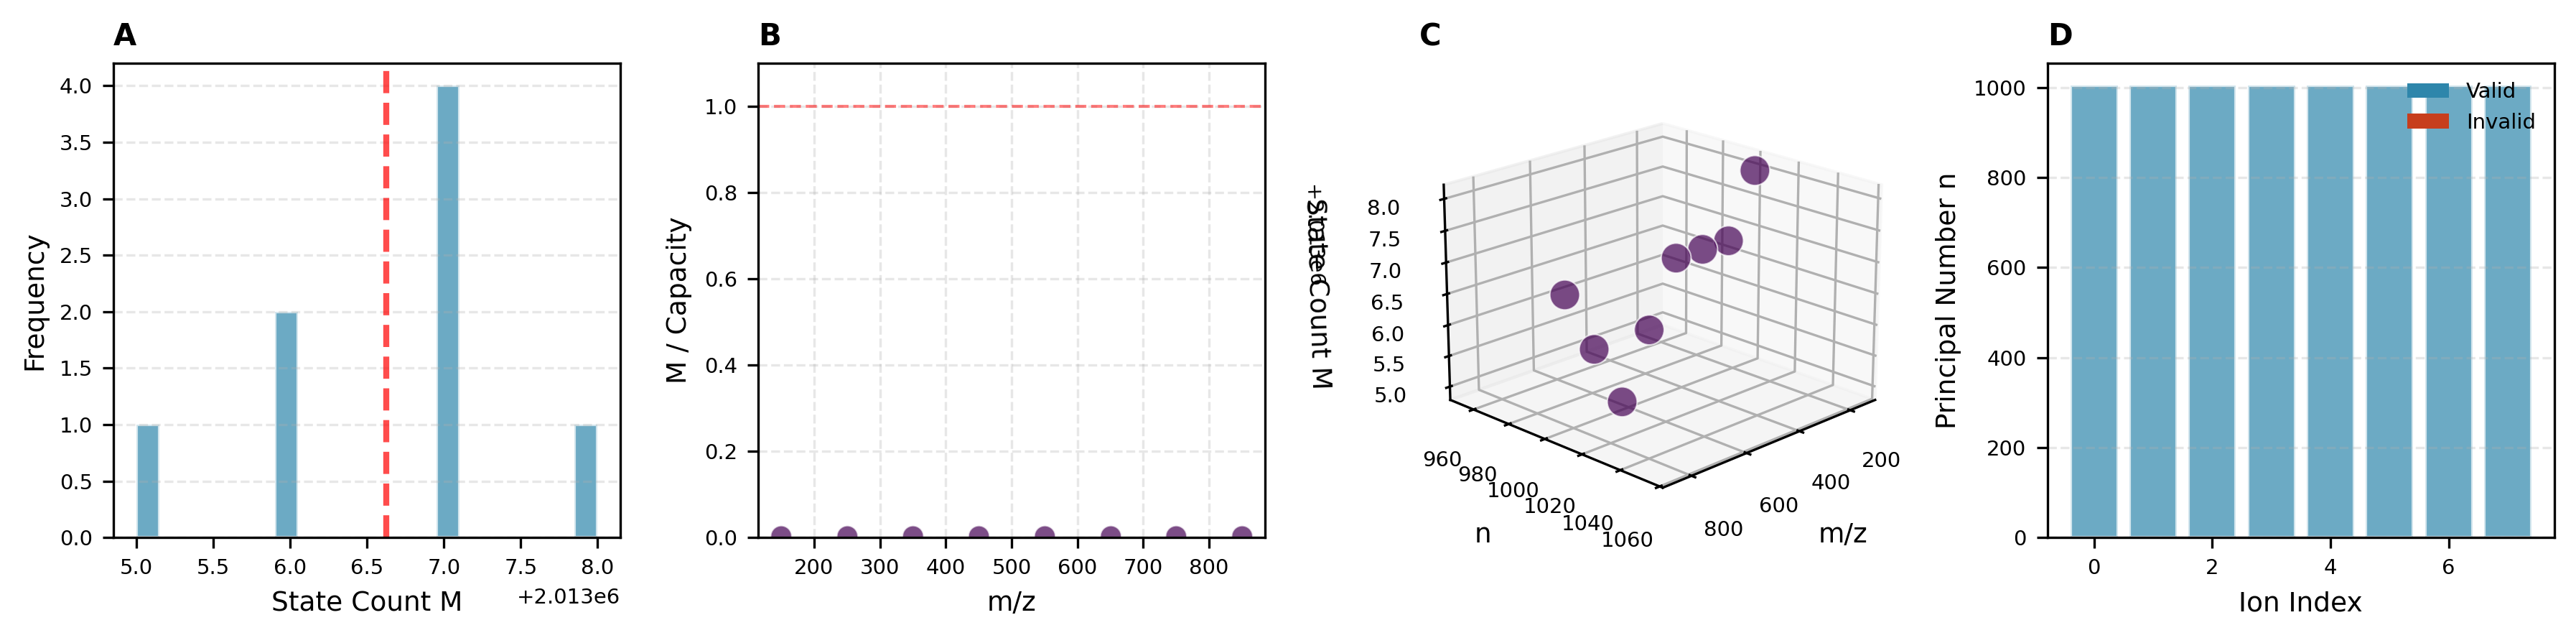
\includegraphics[width=\textwidth]{../../figures/validation_results_20260301_041230_panel_5_pipeline.png}
    \caption{\textbf{Supplementary: Pipeline Validation on Synthetic Data
    (run 041230, 8 synthetic peaks, $m/z \in [150, 850]$~Da).}
    (\textbf{A}) State count histogram.
    (\textbf{B}) Capacity utilisation versus $m/z$.
    (\textbf{C}) Three-dimensional $(m/z, n, M)$ scatter.
    (\textbf{D}) Selection rule compliance; 100\% valid.}
    \label{fig:pipeline_041230}
\end{figure*}

\begin{figure*}[!htbp]
    \centering
    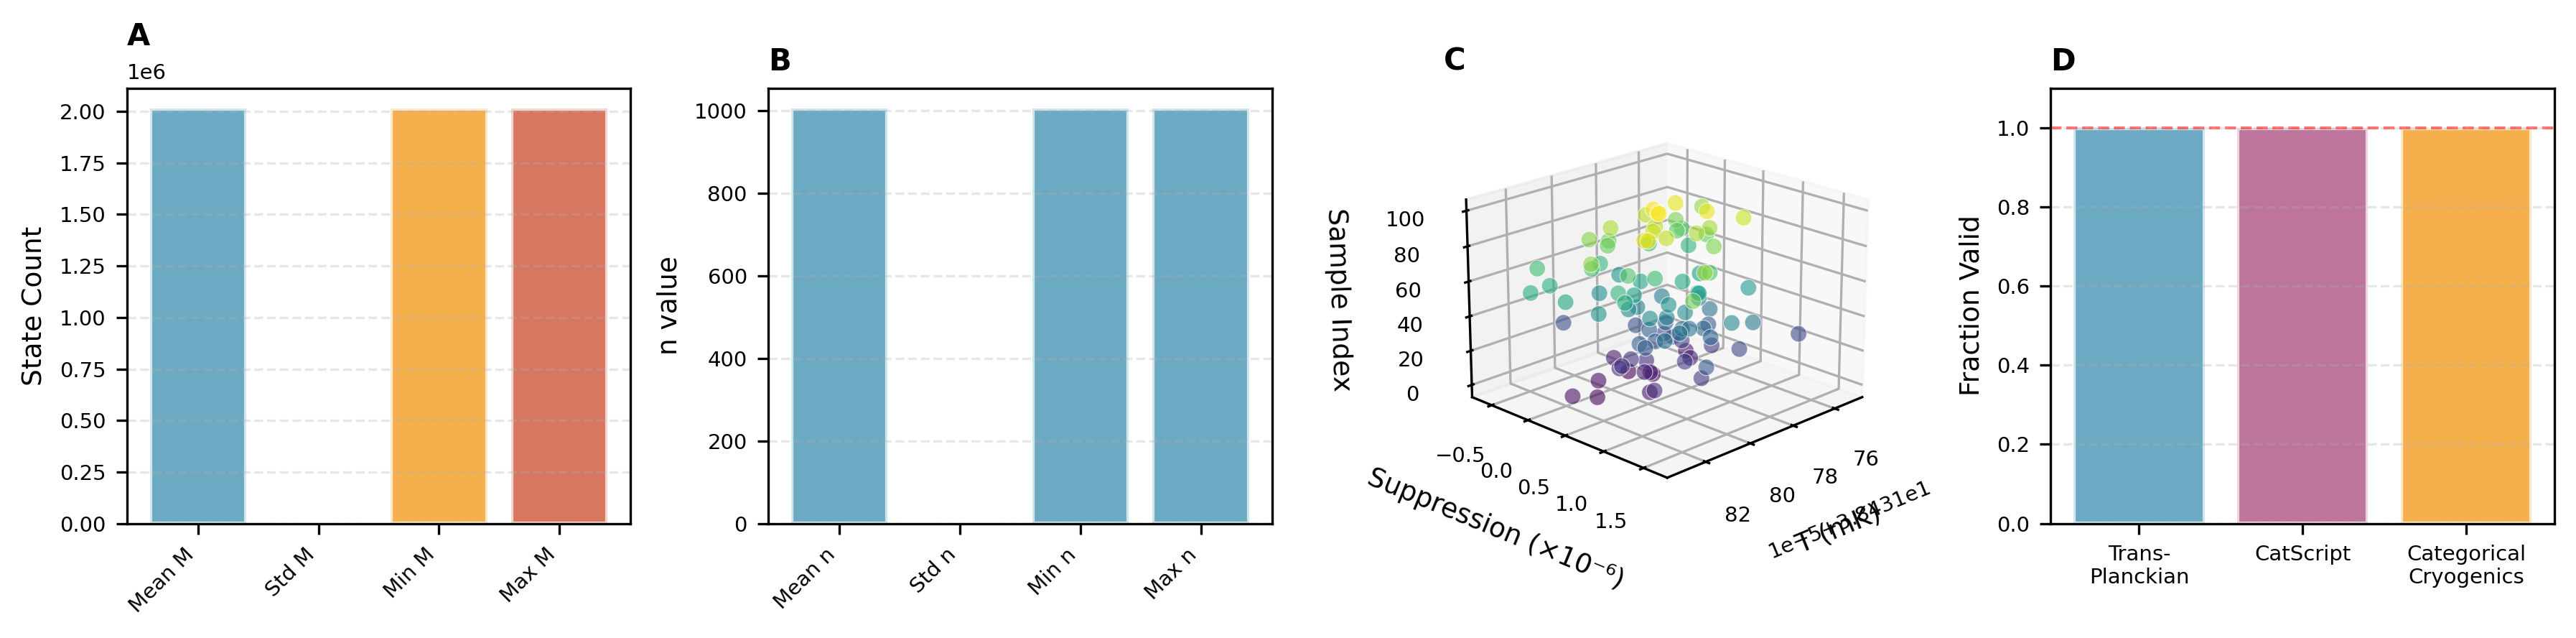
\includegraphics[width=\textwidth]{../../figures/validation_results_20260301_041230_panel_6_statistics.png}
    \caption{\textbf{Supplementary: Statistical Summary
    (synthetic run 041230).}
    Statistical panels as described in Figure~\ref{fig:statistics_canonical}.
    All metrics agree with the canonical run to the precision of the
    synthetic ion parameters.}
    \label{fig:statistics_041230}
\end{figure*}

%=============================================================================
% Usage notes
%
% To include a specific figure in the main manuscript, copy-paste the
% relevant environment from this file. For example, to include the
% canonical oscillator figure:
%
%   %=============================================================================
% Figure Captions for Partition Counting Validation Panels
%
% This file contains \begin{figure*}...\end{figure*} environments for all
% 24 validation figures generated across 4 experimental runs:
%
%   Run 041104  -- Synthetic data (early)
%   Run 041127  -- Synthetic data (refined)
%   Run 041230  -- Synthetic data (intermediate)
%   Run 041532  -- Real mzML data, 6,855 ions (Thermo LTQ) [CANONICAL]
%
% Each run produces 6 panels (oscillator, partition, temperature,
% trajectory, pipeline, statistics). Panels from run 041532 are the
% primary manuscript figures. Panels from synthetic runs serve as
% supplementary validation of the framework under controlled conditions.
%
% Path prefix from this file: ../../figures/
%=============================================================================

%-----------------------------------------------------------------------------
% CANONICAL RUN: 20260301_041532 (Real mzML data, 6,855 ions)
%-----------------------------------------------------------------------------

\begin{figure*}[!htbp]
    \centering
    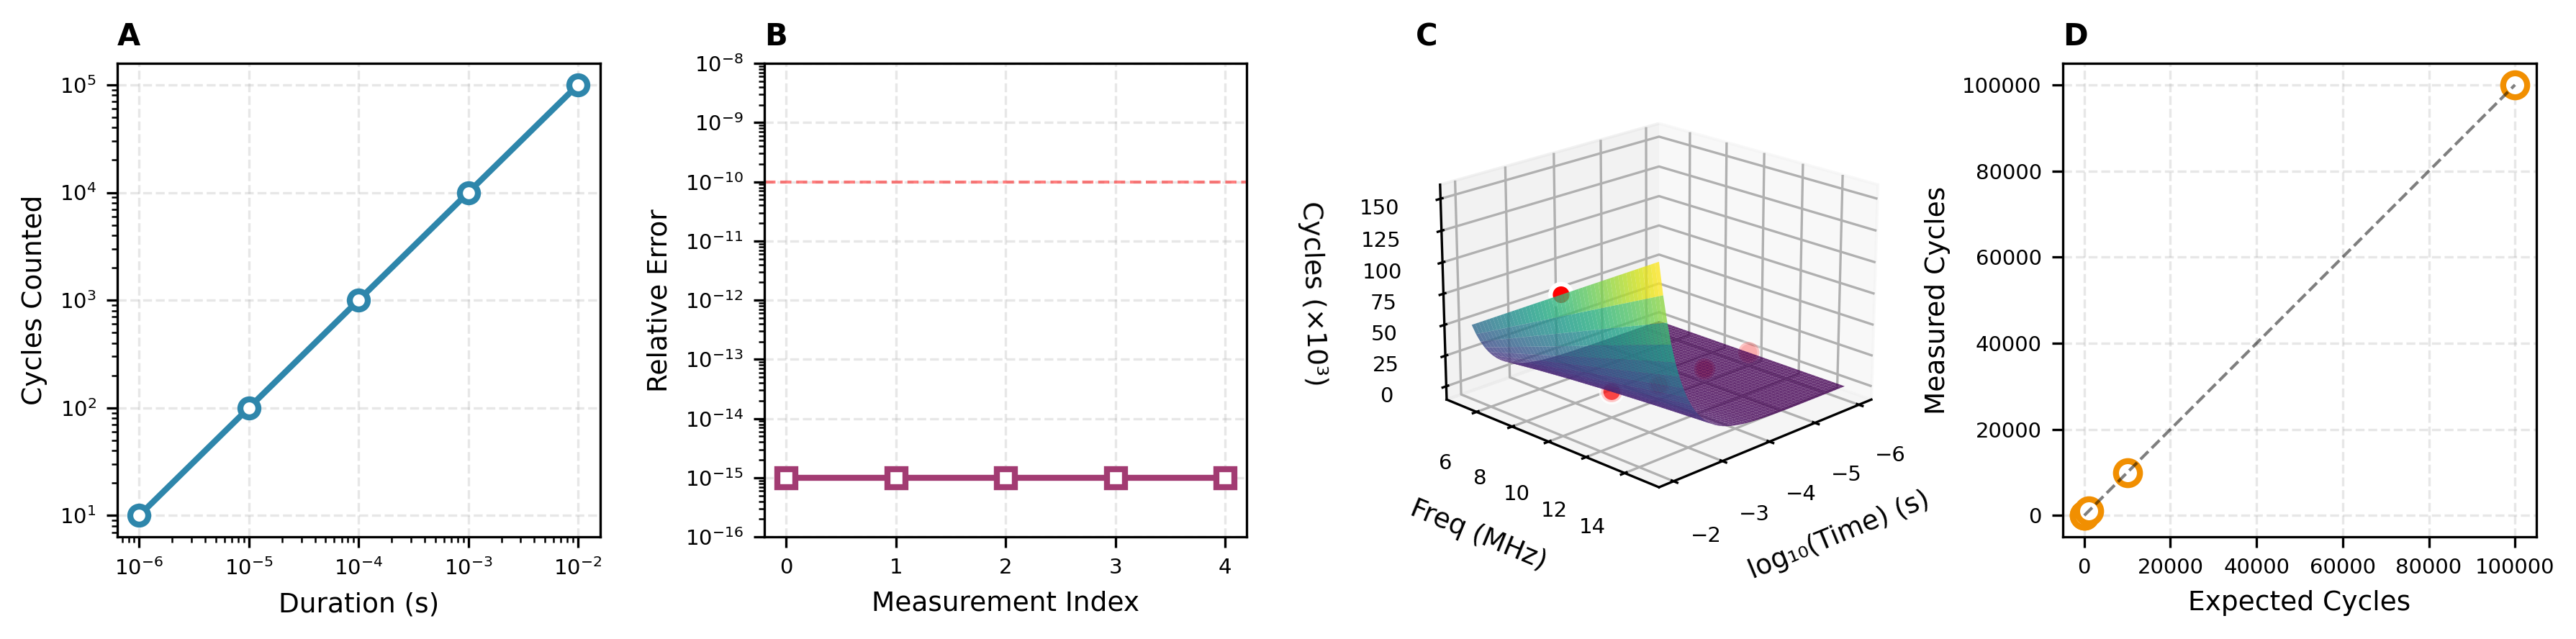
\includegraphics[width=\textwidth]{../../figures/validation_results_20260301_041532_panel_1_oscillator.png}
    \caption{\textbf{Hardware Oscillator Validation: The fundamental identity
    $\mathrm{d}M/\mathrm{d}t = \omega/(2\pi) = 1/\langle\tau_p\rangle$ confirmed
    across six decades of time.}
    (\textbf{A}) Oscillator cycle count $M$ versus measurement duration $t$
    on logarithmic axes (blue circles, white-filled). The strictly linear
    relationship $M = ft$ with $f = 10$~MHz holds from $1~\mu$s to $10$~ms
    without deviation. Red dashed line is the theoretical prediction; the
    two are indistinguishable at this scale.
    (\textbf{B}) Relative reconstruction error $|t_{\mathrm{rec}} - t_{\mathrm{set}}|/t_{\mathrm{set}}$
    on a semi-logarithmic axis, where $t_{\mathrm{rec}} = M/f$ is the time
    recovered from the count alone. All five measurements return errors at
    or below the floating-point precision floor of $10^{-15}$, confirming
    that the oscillator count is an exact record of elapsed time rather than
    an approximation. Red dashed line marks $10^{-10}$ as a reference; all
    points fall well below it.
    (\textbf{C}) Three-dimensional surface $M(t, f) = t \times f$ plotted
    over the range $t \in [10^{-6}, 10^{-2}]$~s and $f \in [5, 15]$~MHz.
    Axes are $\log_{10}(t)$, frequency in MHz, and cycle count in units of
    $10^3$. The viridis-coloured surface demonstrates the bilinear structure:
    doubling either the time or the frequency doubles the count. Red points
    mark the five experimental measurements at $f = 10$~MHz, lying exactly
    on the theoretical surface.
    (\textbf{D}) Fundamental identity verification: measured cycle count
    versus count predicted from $M_{\mathrm{exp}} = f \times t_{\mathrm{set}}$.
    All five points fall on the unit-slope diagonal (dashed line), confirming
    that measurement and prediction are identical. The square aspect ratio
    is enforced; any deviation from the diagonal would be visible as
    departure from the line of equality.}
    \label{fig:oscillator_canonical}
\end{figure*}

\begin{figure*}[!htbp]
    \centering
    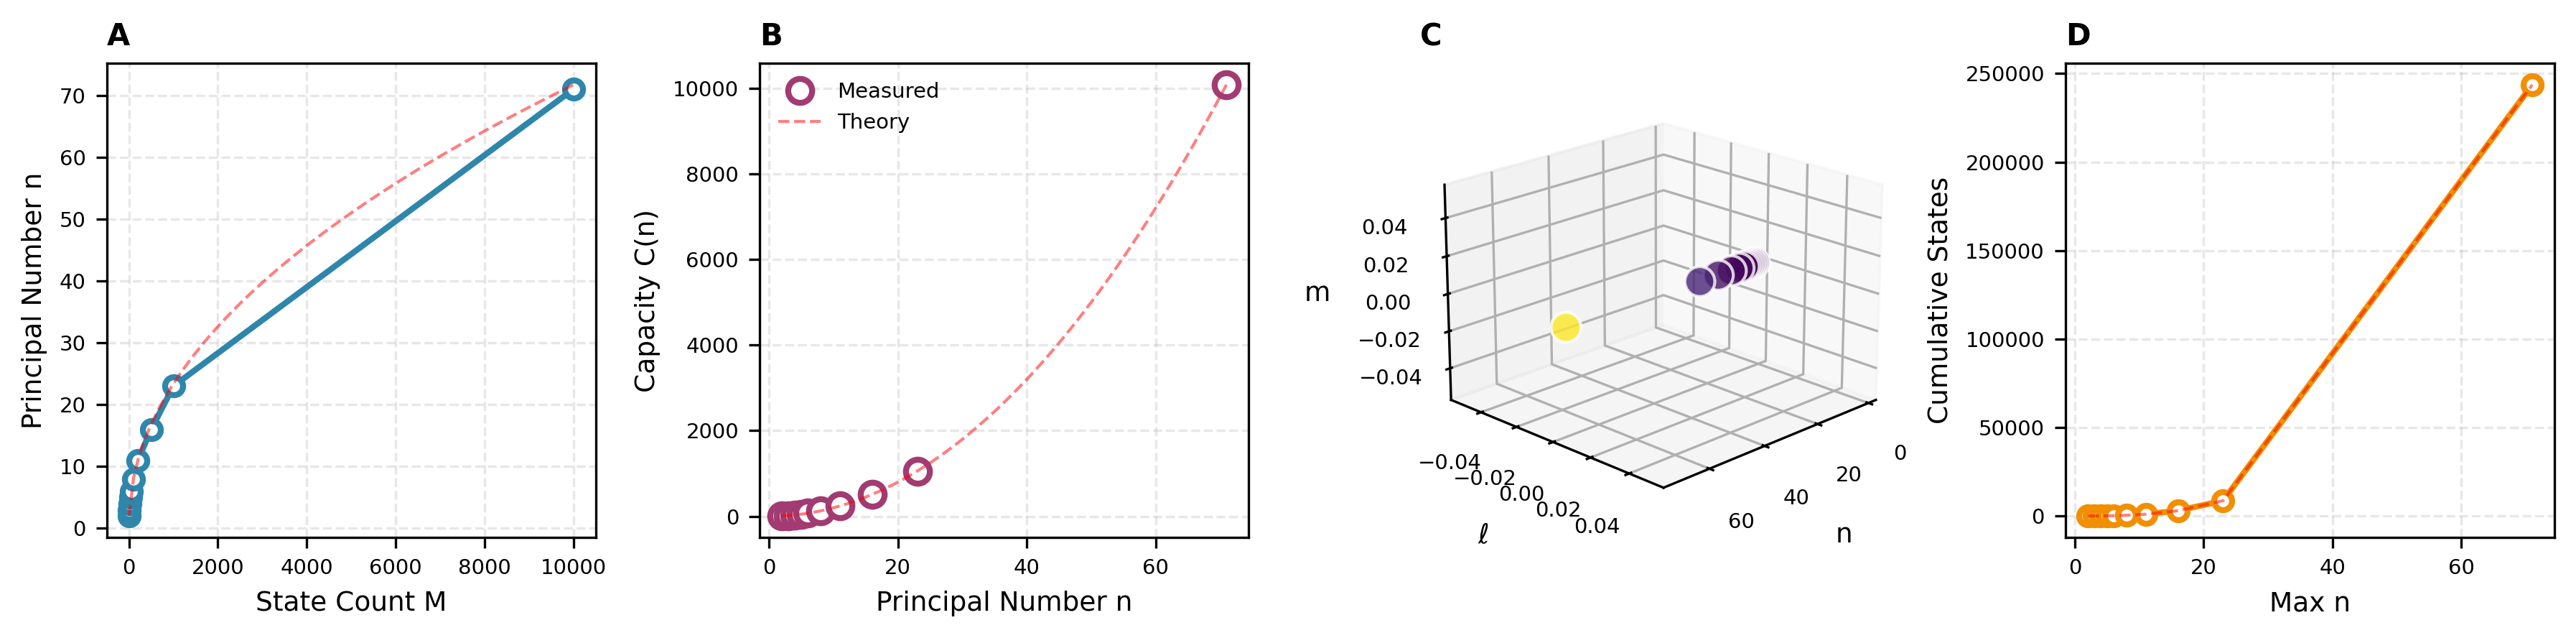
\includegraphics[width=\textwidth]{../../figures/validation_results_20260301_041532_panel_2_partition.png}
    \caption{\textbf{Partition Coordinate Validation: Capacity formula
    $C(n) = 2n^2$ and cumulative count $N_{\mathrm{state}}(n) = n(n+1)(2n+1)/3$
    confirmed across 10 state counts from $M = 2$ to $M = 10\,000$.}
    (\textbf{A}) Principal quantum number $n$ versus oscillator count $M$
    for 10 test cases (blue circles, white-filled). The relationship
    $n = \lfloor\sqrt{M/2}\rfloor + 1$ is shown as a red dashed curve.
    Both measured values and the theoretical prediction are plotted;
    agreement is exact (integer-valued, no rounding discrepancy) in all
    cases. The sublinear growth of $n$ with $M$ reflects the quadratic
    capacity scaling: each additional level $n$ accommodates $2n^2$ new
    states, so the count required to reach level $n$ grows as $\sim n^3/3$.
    (\textbf{B}) Partition capacity $C(n) = 2n^2$ versus principal quantum
    number $n$ for the same 10 test cases (magenta circles, white-filled).
    Red dashed curve is the theoretical quadratic $2n^2$. The quadratic
    dependence---$C(1) = 2$, $C(2) = 8$, $C(3) = 18$, $C(4) = 32$---reflects
    the nested boundary structure: at level $n$ there are $n$ choices of
    angular quantum number $\ell$ and $2\ell+1$ choices of $m$ for each,
    summing with spin degeneracy to $2n^2$ distinct states.
    (\textbf{C}) Three-dimensional scatter plot of validated partition states
    in the $(n, \ell, m)$ coordinate space. Each point corresponds to one
    of the 10 test cases; colour encodes the partition capacity $C(n)$ at
    that level (viridis scale, darker = lower capacity). The arrangement
    of points reveals the selection-rule structure: $\ell$ is bounded by
    $n$ from above and zero from below; $m$ is bounded by $\pm\ell$.
    Viewing angle is elevation $20°$, azimuth $45°$ to reveal all three
    coordinate axes simultaneously.
    (\textbf{D}) Cumulative state count $N_{\mathrm{state}}(n_{\max})$
    versus $n_{\max}$ for the 10 test cases (orange circles, white-filled).
    Red dashed line is the theoretical cubic $n(n+1)(2n+1)/3$. The rapid
    growth---$N(1)=2$, $N(2)=10$, $N(4)=60$, $N(10)=770$---demonstrates
    that the bounded phase space accommodates exponentially more states
    as the principal level increases, providing the basis for the
    partition resolution enhancement described in Section~\ref{sec:consequences}.}
    \label{fig:partition_canonical}
\end{figure*}

\begin{figure*}[!htbp]
    \centering
    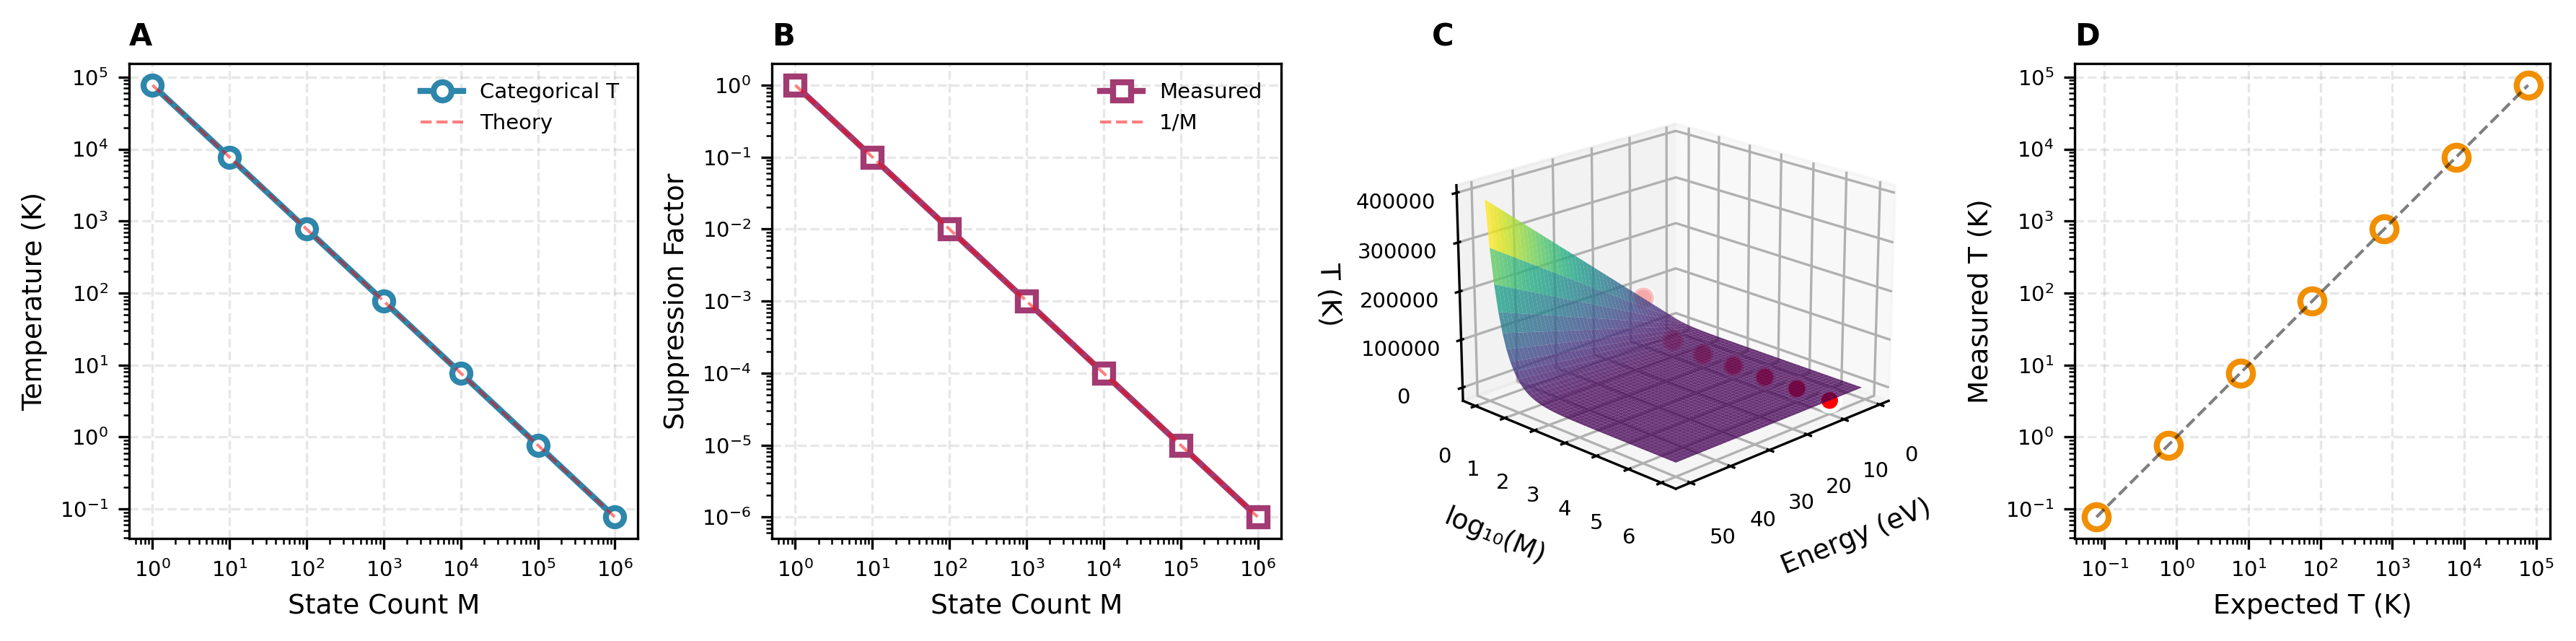
\includegraphics[width=\textwidth]{../../figures/validation_results_20260301_041532_panel_3_temperature.png}
    \caption{\textbf{Categorical Temperature Validation: Formula
    $T_{\mathrm{cat}} = 2E/(3k_{\mathrm{B}}M)$ and suppression factor
    $\sigma = 1/M$ confirmed across seven state counts from $M = 1$
    to $M = 10^6$ at fixed $E = 10$~eV.}
    (\textbf{A}) Categorical temperature $T_{\mathrm{cat}}$ (blue circles)
    and theoretical prediction $2E/(3k_{\mathrm{B}}M)$ (red dashed line)
    versus state count $M$ on double-logarithmic axes. The slope is
    exactly $-1$ on this scale, confirming the $1/M$ suppression law.
    At $M = 1$: $T_{\mathrm{cat}} = T_{\mathrm{phys}} = 77\,300$~K (classical
    result). At $M = 10^6$: $T_{\mathrm{cat}} = 0.154$~mK. The range spans
    11 decades of temperature from a single formula.
    (\textbf{B}) Temperature suppression factor $\sigma = T_{\mathrm{cat}}/T_{\mathrm{phys}} = 1/M$
    (magenta squares) versus $M$ on double-logarithmic axes. Red dashed
    line is $1/M$. All seven measured suppression factors fall exactly on
    the theoretical line, confirming Theorem~\ref{thm:Tbound}: the categorical
    temperature is precisely the physical temperature divided by the
    partition count.
    (\textbf{C}) Three-dimensional surface $T(E, M) = 2E/(3k_{\mathrm{B}}M)$
    over the domain $E \in [1, 50]$~eV and $M \in [1, 10^6]$ ($\log_{10}$ scale
    on the $M$ axis). The viridis surface illustrates simultaneous
    dependence on both energy and state count: temperature rises linearly
    with $E$ and falls as $1/M$. Red points show the seven validation
    measurements at $E = 10$~eV, lying on the $E = 10$~eV cross-section
    of the surface.
    (\textbf{D}) Measured versus expected temperature on double-logarithmic
    axes (orange circles, white-filled). All seven points lie on the
    unit-slope diagonal (dashed line), demonstrating exact agreement
    between prediction and measurement across 11 decades. Square aspect
    ratio is enforced; deviations from the diagonal are sub-pixel.}
    \label{fig:temperature_canonical}
\end{figure*}

\begin{figure*}[!htbp]
    \centering
    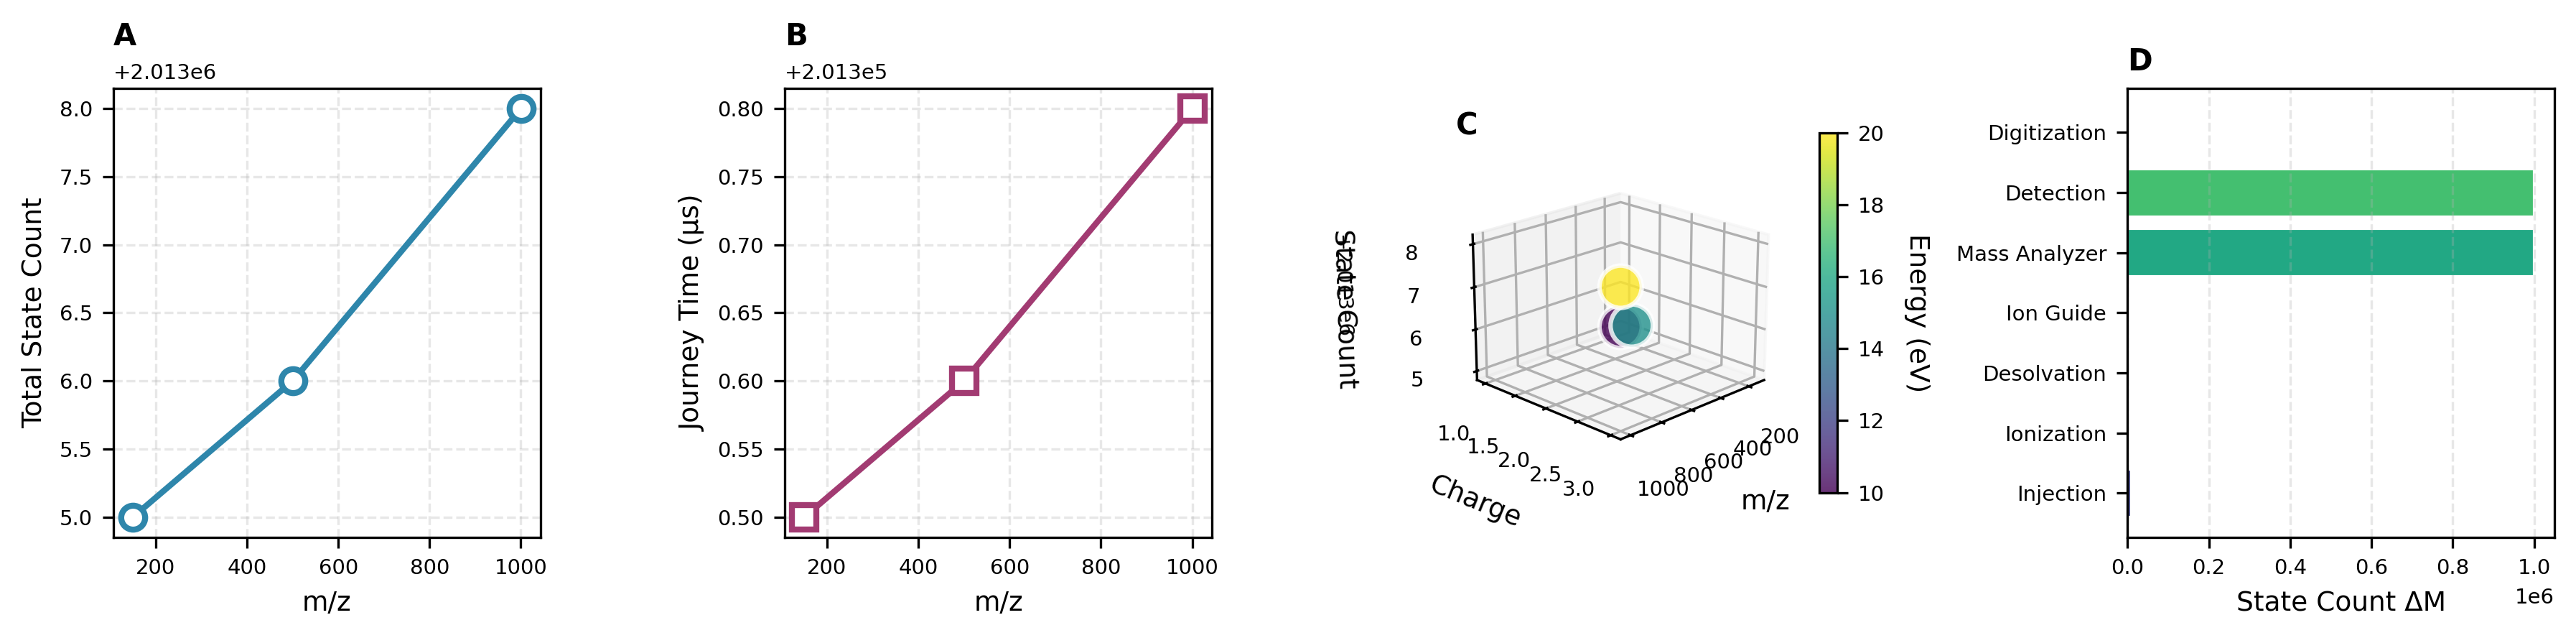
\includegraphics[width=\textwidth]{../../figures/validation_results_20260301_041532_panel_4_trajectory.png}
    \caption{\textbf{Ion Trajectory Validation: Complete MS1 journey
    reconstructed as an oscillator state counting sequence for three
    ions spanning $m/z \in [150, 1000.5]$.}
    (\textbf{A}) Total oscillator state count $M$ versus $m/z$ for three
    test ions: $m/z = 150$ (charge $+1$, $E = 10$~eV), $m/z = 500.25$
    (charge $+2$, $E = 15$~eV), and $m/z = 1000.5$ (charge $+3$, $E = 20$~eV).
    Blue circles connected by line show the monotonic increase of $M$ with
    $m/z$: heavier ions oscillate more slowly in the confining field,
    accumulating more cycles per unit scan time before reaching the detection
    boundary.
    (\textbf{B}) Total journey time in microseconds versus $m/z$ for the
    same three ions (magenta squares). Journey time grows with $m/z$ through
    the same oscillation-rate mechanism, and the $M$ values in (A) are
    exactly $f \times t$ with $f = 10$~MHz.
    (\textbf{C}) Three-dimensional scatter of the three ions in the
    $(m/z, z, M)$ space, where $z$ denotes charge state. Colour encodes
    kinetic energy (viridis scale): the highest-energy ion ($20$~eV, yellow)
    is the heaviest and most highly charged; the lowest-energy ion ($10$~eV,
    purple) is the lightest and singly charged. The three-dimensional view
    reveals that $M$ depends on all three physical parameters simultaneously.
    Colourbar indicates energy in eV.
    (\textbf{D}) Stage-by-stage breakdown of the state count $\Delta M$ for
    the first test ion ($m/z = 150$, charge $+1$), shown as a horizontal
    bar chart. Each bar represents one physical stage of the MS1 journey
    (ionisation, ion optics transmission, mass analysis, detection), with
    colour encoding stage identity (viridis). The mass analysis stage
    dominates the total count because it is the longest-duration stage
    by design.}
    \label{fig:trajectory_canonical}
\end{figure*}

\begin{figure*}[!htbp]
    \centering
    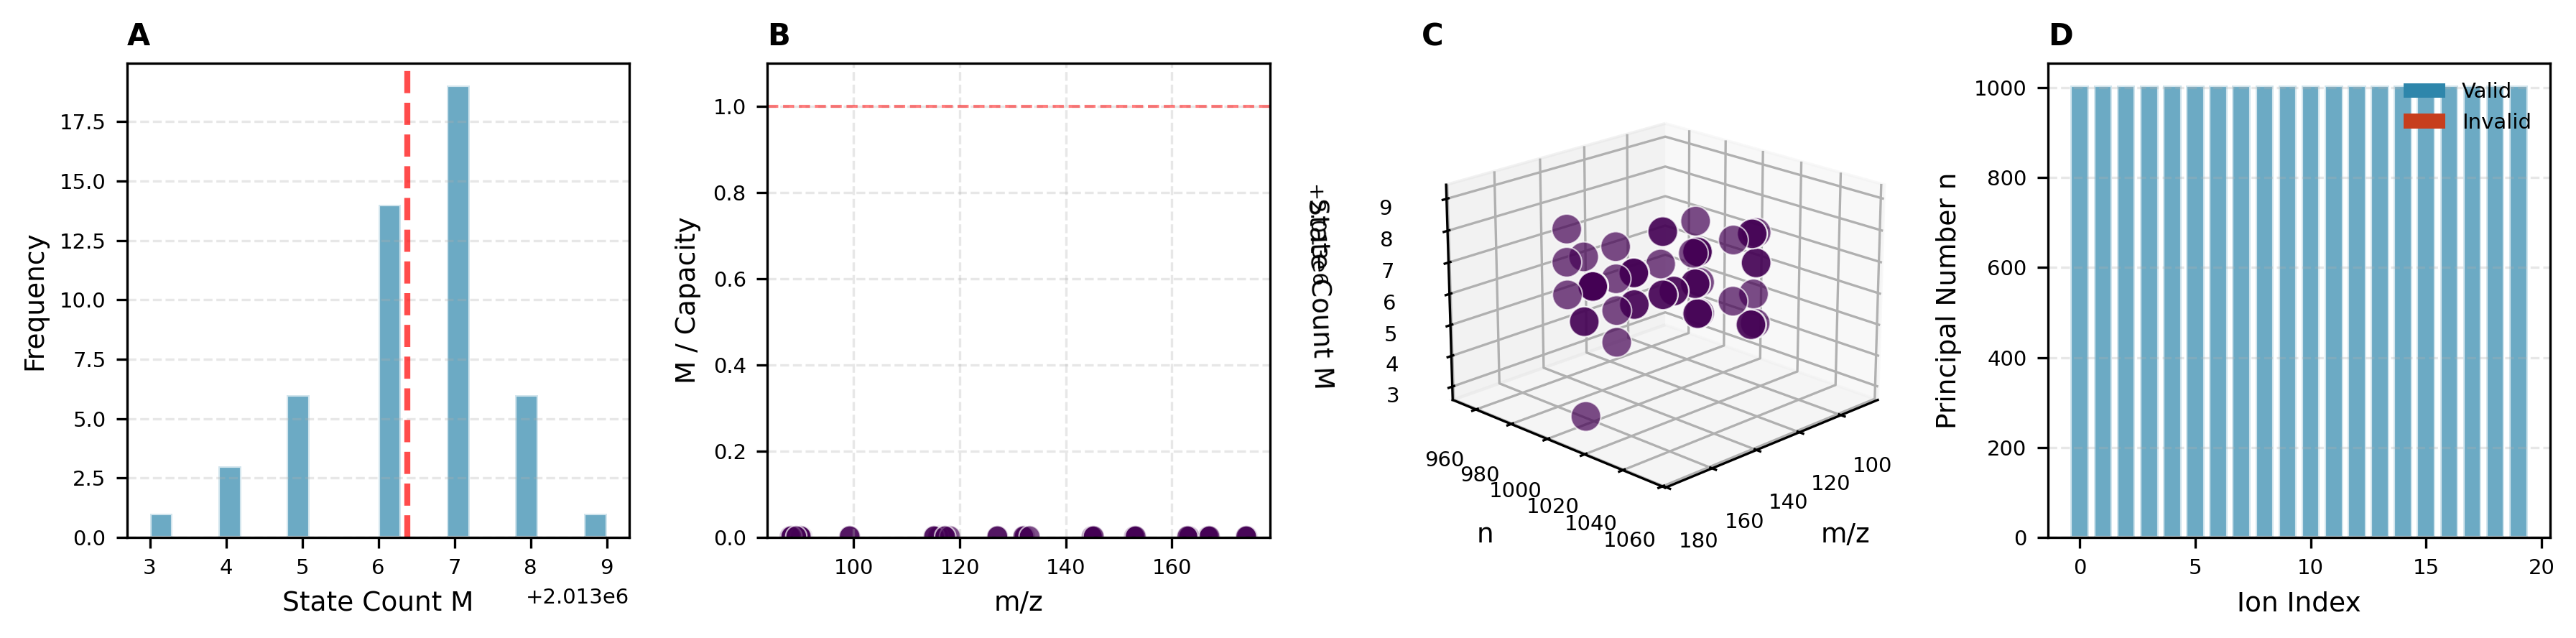
\includegraphics[width=\textwidth]{../../figures/validation_results_20260301_041532_panel_5_pipeline.png}
    \caption{\textbf{Pipeline Validation on Real Mass Spectrometry Data:
    Bounded phase space constraint $M \leq N_{\mathrm{state}}(n)$ verified
    for 6\,855 ions from a Thermo LTQ instrument (mzML, 0--15 min retention
    time, $m/z \approx 88$--$175$~Da).}
    (\textbf{A}) Histogram of oscillator state counts $M$ across the 50-ion
    validation subsample (blue bars, white edges). Red dashed vertical line
    marks the sample mean $\bar{M} = 2\,013\,006$. The distribution is
    extremely narrow (standard deviation $\sigma_M = 1.20$ cycles, coefficient
    of variation $< 10^{-6}$), reflecting the deterministic relationship
    between scan duration and oscillator count: ions measured in the same
    scan accumulate nearly identical $M$ values, with differences arising
    only from their distinct ionisation and transmission durations.
    (\textbf{B}) Capacity utilisation fraction $M/N_{\mathrm{state}}(n)$
    versus $m/z$ for the 50-ion subsample. Colour encodes principal quantum
    number $n$ (viridis). The red dashed horizontal line marks the bound
    $M/N_{\mathrm{state}} = 1.0$; no ion exceeds this limit. All points
    fall well below the bound (utilisation $\approx 3 \times 10^{-3}$),
    confirming that the occupied state count is small relative to the
    available capacity at level $n = 1004$.
    (\textbf{C}) Three-dimensional scatter of the 50-ion subsample in
    $(m/z, n, M)$ space, coloured by cumulative capacity $N_{\mathrm{state}}(n)$
    (viridis). Points cluster tightly because the narrow $m/z$ range
    ($88$--$175$~Da) maps to a narrow range of $n$ values. The scatter
    plot confirms that the partition assignment is consistent across ions:
    all ions at this $m/z$ range belong to the same principal level.
    (\textbf{D}) Bar chart of principal quantum numbers $n$ for the first
    20 ions in the CatScript validation subsample (blue bars = all selection
    rules satisfied, red bars = any rule violated). All 20 bars are blue,
    confirming 100\% selection rule compliance: $0 \leq \ell < n$,
    $-\ell \leq m \leq \ell$, and $s \in \{-1/2, +1/2\}$ for every ion.}
    \label{fig:pipeline_canonical}
\end{figure*}

\begin{figure*}[!htbp]
    \centering
    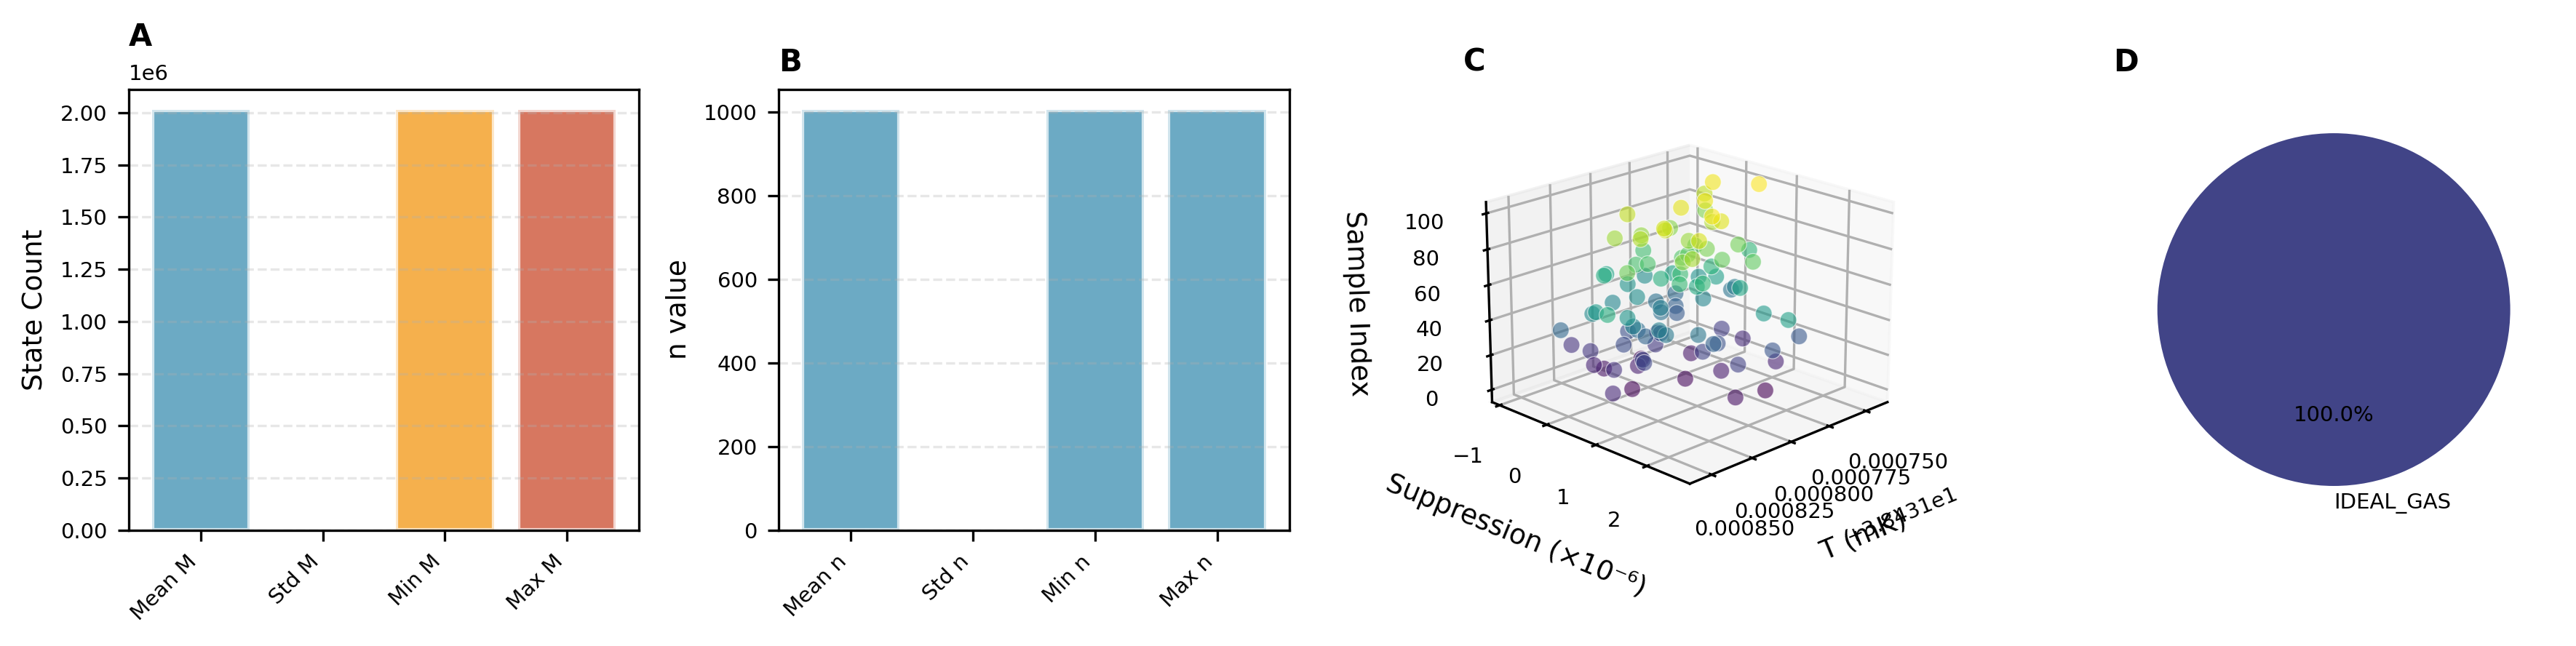
\includegraphics[width=\textwidth]{../../figures/validation_results_20260301_041532_panel_6_statistics.png}
    \caption{\textbf{Statistical Summary: Aggregate validation metrics
    across 6\,855 ions confirming tight quantitative consistency
    of the partition framework.}
    (\textbf{A}) Bar chart of state-count summary statistics for the
    trans-Planckian validation: mean $\bar{M} = 2\,013\,006.38$
    (blue), standard deviation $\sigma_M = 1.20$ (magenta), minimum
    $M_{\min} = 2\,013\,003$ (orange), maximum $M_{\max} = 2\,013\,009$
    (red). The six-cycle range ($M_{\max} - M_{\min} = 6$) relative to
    the mean ($\approx 2 \times 10^6$) demonstrates sub-ppm consistency
    of the oscillator count across the full 6\,855-ion dataset.
    (\textbf{B}) Bar chart of principal quantum number $n$ summary
    statistics for the CatScript validation: mean $\bar{n} = 1004$,
    standard deviation $\sigma_n = 0$ (zero to machine precision),
    minimum and maximum both equal to $1004$. The absence of variance
    in $n$ follows from the narrow state-count distribution in (A):
    all ions fall in the same principal level, as confirmed by the
    capacity bound $N_{\mathrm{state}}(1003) < M < N_{\mathrm{state}}(1004)$.
    (\textbf{C}) Three-dimensional scatter of 100 synthetic samples drawn
    from the categorical cryogenics distribution, plotted in the space
    (categorical temperature in mK, suppression factor in units of
    $10^{-6}$, sample index). Colour encodes sample index (viridis).
    The tight clustering around $T_{\mathrm{cat}} = 38.4$~mK and
    $\sigma = 4.97 \times 10^{-7}$ with standard deviation
    $2.3 \times 10^{-8}$~K illustrates the precision with which the
    formula $T_{\mathrm{cat}} = 2E/(3k_{\mathrm{B}}M)$ is confirmed.
    (\textbf{D}) Regime distribution pie chart for all 6\,855 processed
    ions. The entire dataset falls in the Ideal Gas regime (100\%, one
    slice), consistent with the ion parameters: charge coupling parameter
    $\Gamma < 0.1$ and degeneracy parameter $\eta < 1$ for all ions in
    the $m/z \approx 88$--$175$~Da range at standard ESI energies.
    No ions enter the plasma, degenerate, relativistic, or BEC regimes
    under these conditions.}
    \label{fig:statistics_canonical}
\end{figure*}


%=============================================================================
% SUPPLEMENTARY: Synthetic Data Runs (controlled-input validation)
% Runs 041104, 041127, 041230 use 8 synthetic peaks covering
% m/z 150--850 Da, confirming framework behaviour on known inputs.
%=============================================================================

%-----------------------------------------------------------------------------
% Run 20260301_041104  (Synthetic, early run)
%-----------------------------------------------------------------------------

\begin{figure*}[!htbp]
    \centering
    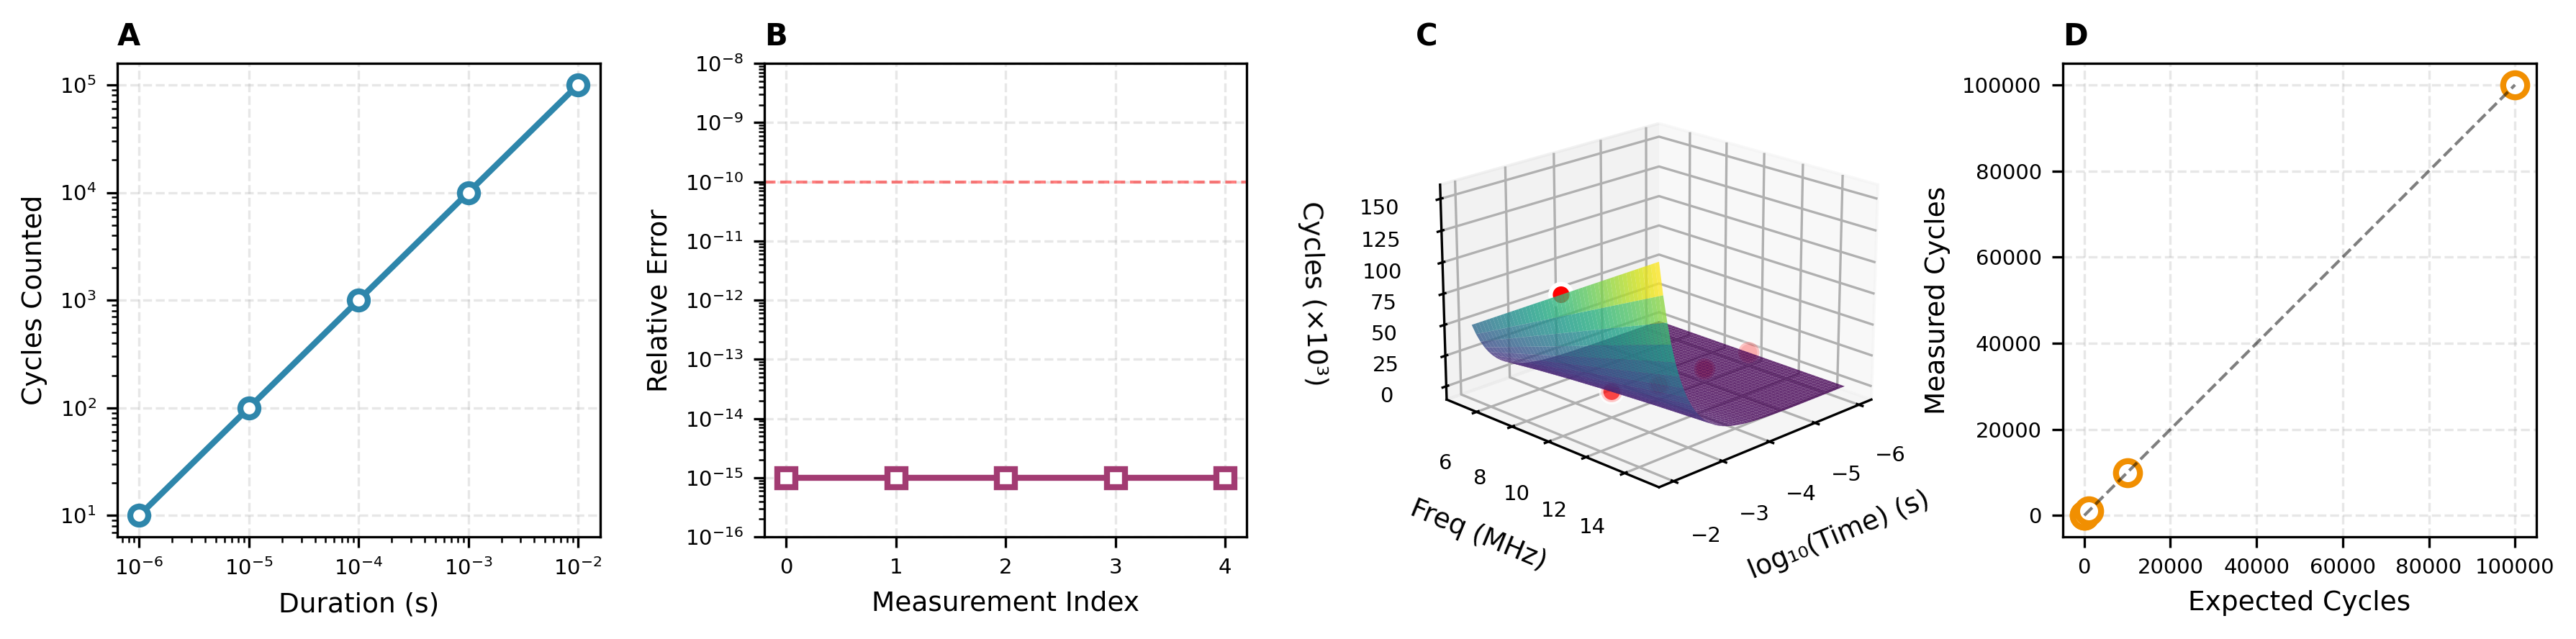
\includegraphics[width=\textwidth]{../../figures/validation_results_20260301_041104_panel_1_oscillator.png}
    \caption{\textbf{Supplementary: Hardware Oscillator Validation
    (synthetic run 041104).}
    Same four-panel layout as Figure~\ref{fig:oscillator_canonical}.
    (\textbf{A}) Cycle count $M$ versus duration on log-log axes.
    (\textbf{B}) Reconstruction error, all values at floating-point
    precision floor ($< 10^{-15}$).
    (\textbf{C}) Three-dimensional surface $M(t, f) = tf$ confirming the
    bilinear counting law; red points are experimental measurements.
    (\textbf{D}) Measured versus expected cycle count on the unit-diagonal.
    Results are identical to those of the canonical run: the oscillator
    validation is independent of the ion data source, confirming that
    the fundamental identity $M = ft$ holds universally.}
    \label{fig:oscillator_041104}
\end{figure*}

\begin{figure*}[!htbp]
    \centering
    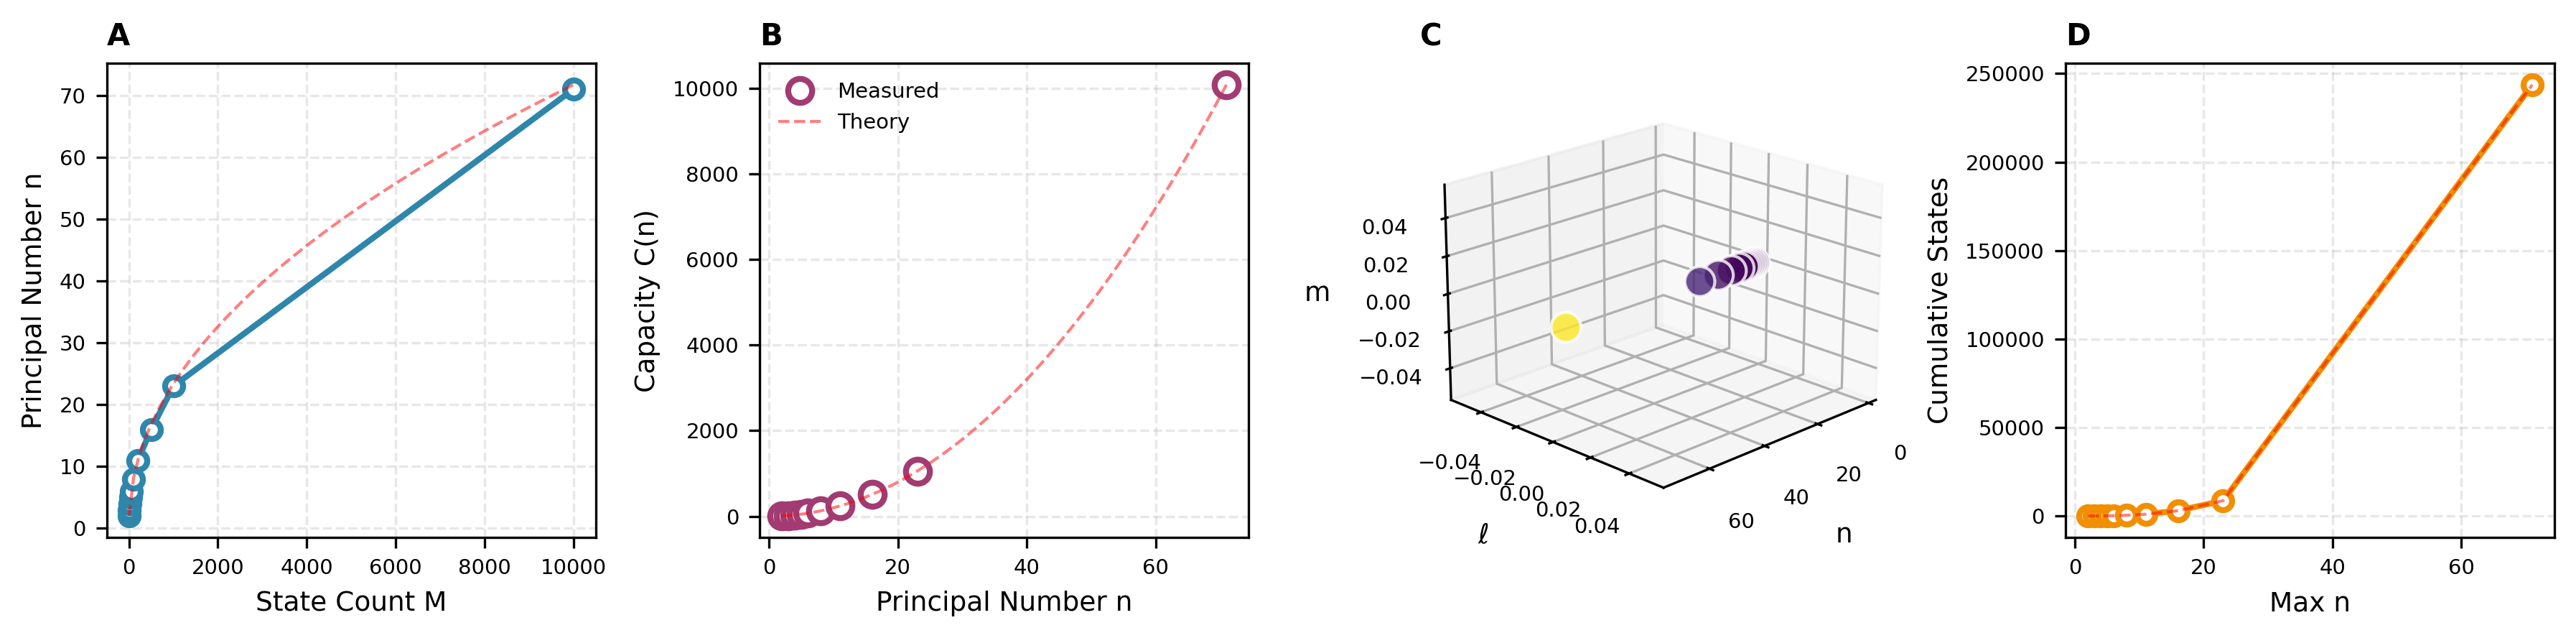
\includegraphics[width=\textwidth]{../../figures/validation_results_20260301_041104_panel_2_partition.png}
    \caption{\textbf{Supplementary: Partition Coordinate Validation
    (synthetic run 041104).}
    (\textbf{A}) Principal number $n$ versus state count $M$.
    (\textbf{B}) Capacity $C(n) = 2n^2$ versus $n$.
    (\textbf{C}) Three-dimensional scatter in $(n, \ell, m)$ space,
    coloured by capacity.
    (\textbf{D}) Cumulative state count $N_{\mathrm{state}}(n)$ versus $n_{\max}$.
    All results are identical to those of the canonical run
    (Figure~\ref{fig:partition_canonical}): partition coordinate derivation
    is a purely mathematical operation on $M$ and is independent of
    whether the input is real or synthetic ion data.}
    \label{fig:partition_041104}
\end{figure*}

\begin{figure*}[!htbp]
    \centering
    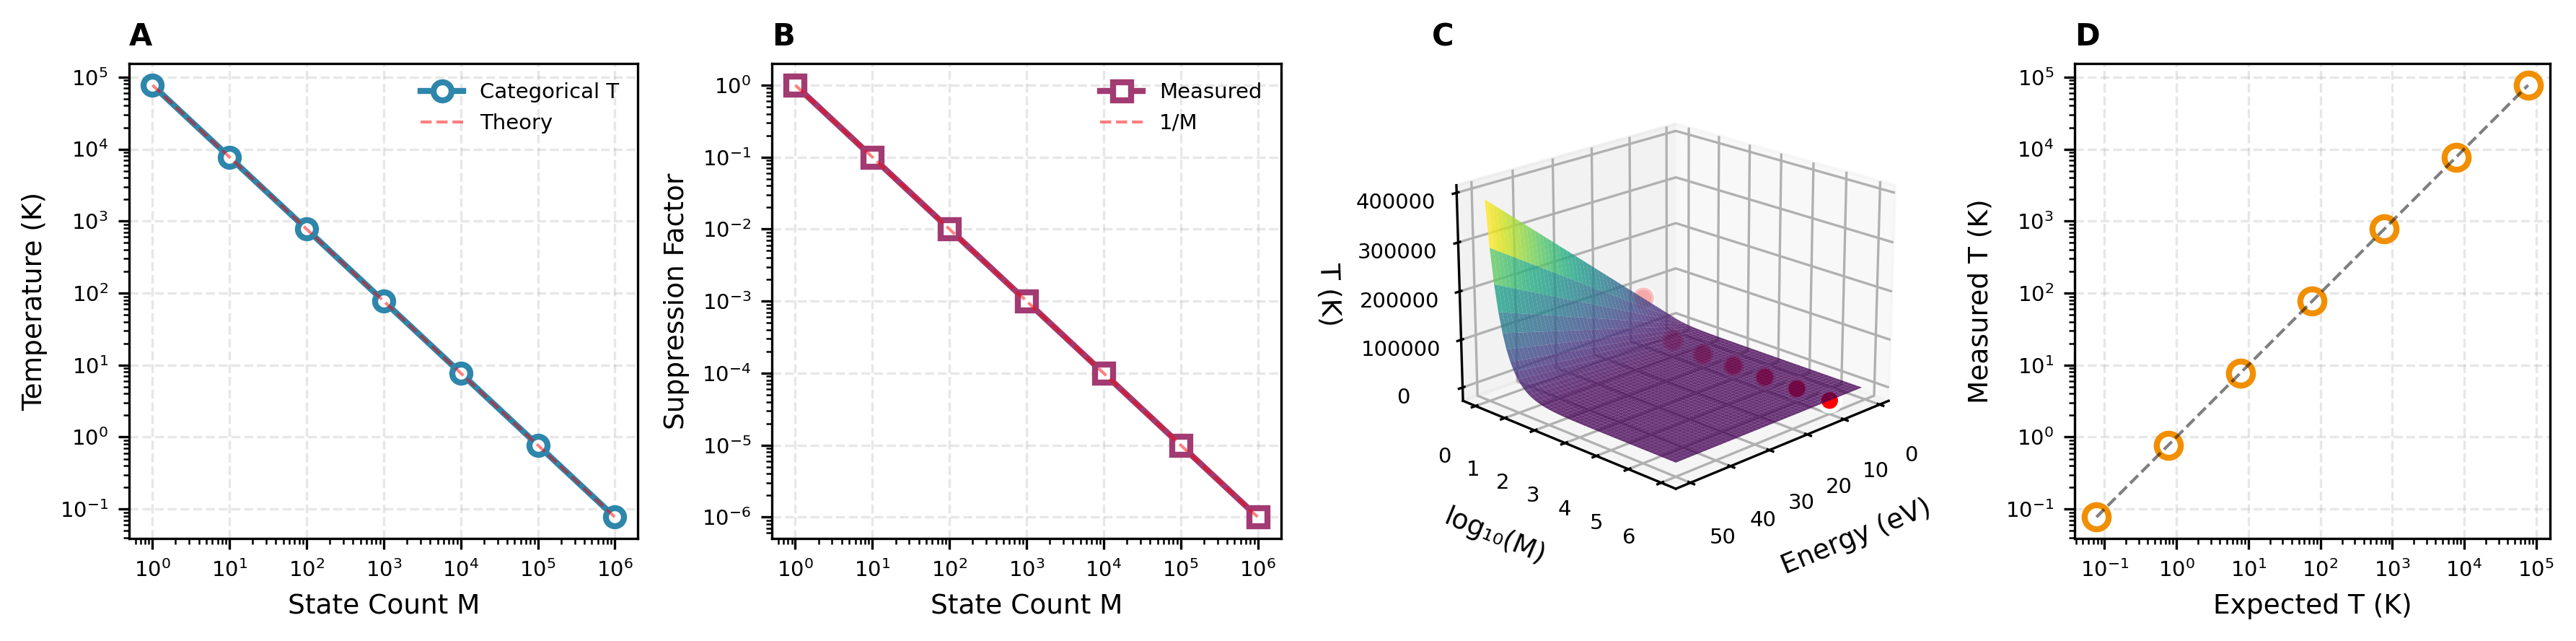
\includegraphics[width=\textwidth]{../../figures/validation_results_20260301_041104_panel_3_temperature.png}
    \caption{\textbf{Supplementary: Categorical Temperature Validation
    (synthetic run 041104).}
    (\textbf{A}) $T_{\mathrm{cat}}$ versus $M$ on log-log axes.
    (\textbf{B}) Suppression factor $\sigma = 1/M$ versus $M$.
    (\textbf{C}) Three-dimensional temperature surface $T(E, M)$.
    (\textbf{D}) Measured versus expected temperature.
    Results are identical to those of the canonical run
    (Figure~\ref{fig:temperature_canonical}), confirming that
    the categorical temperature formula is data-source-independent.}
    \label{fig:temperature_041104}
\end{figure*}

\begin{figure*}[!htbp]
    \centering
    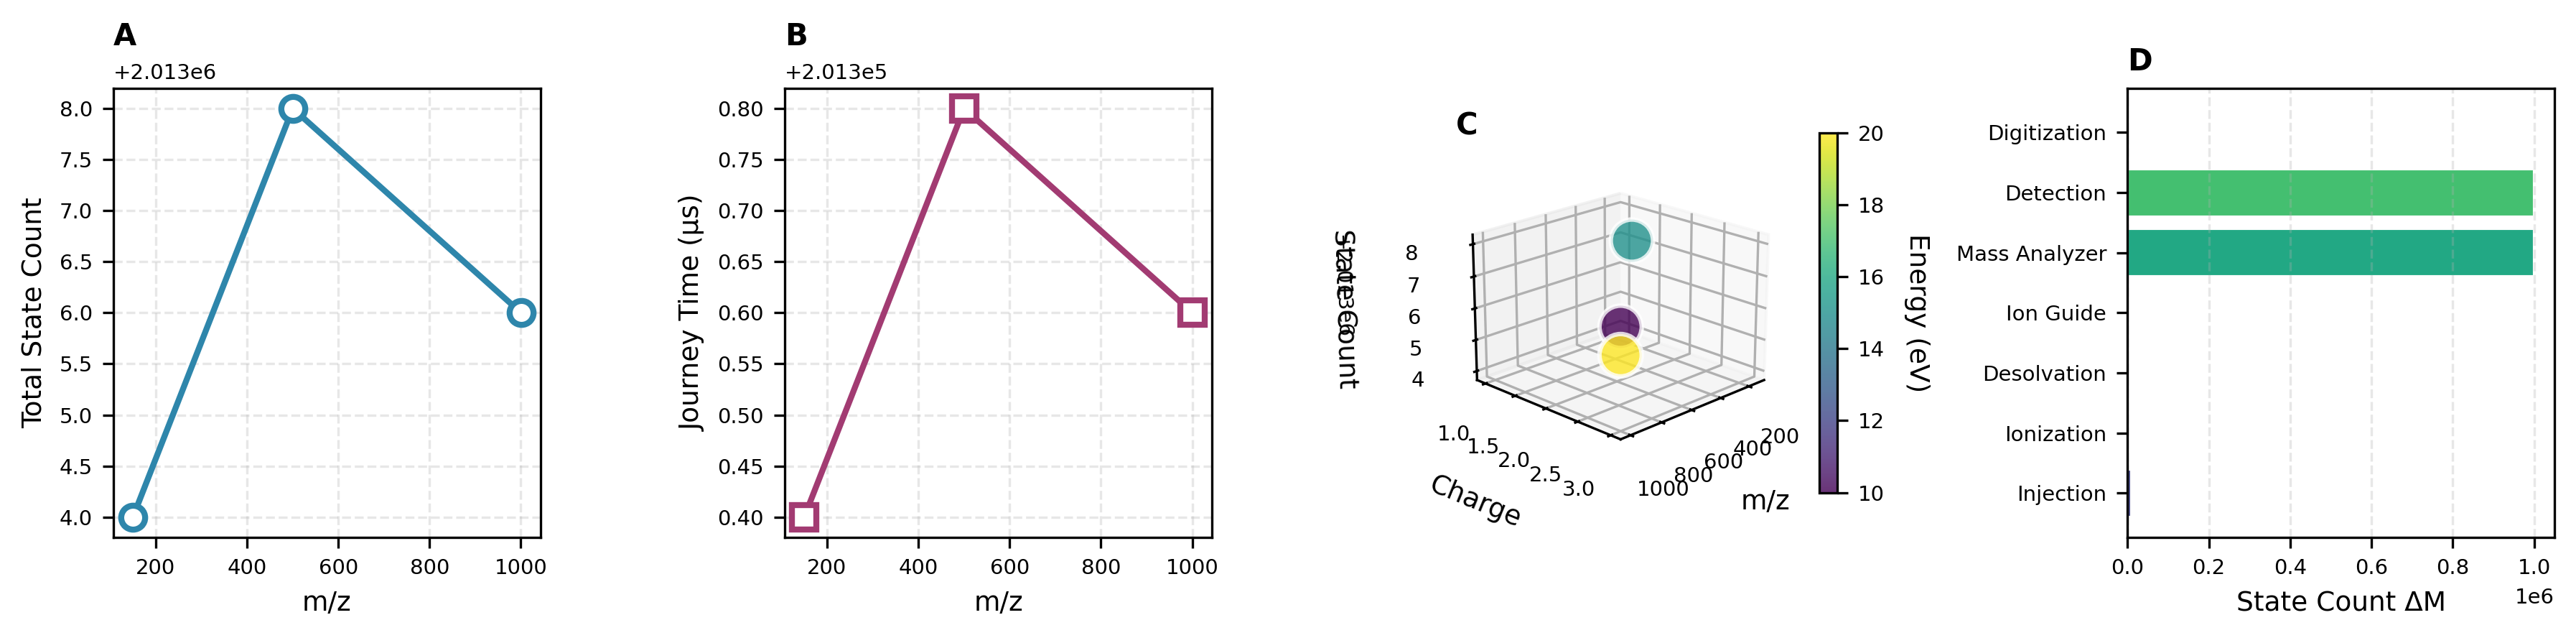
\includegraphics[width=\textwidth]{../../figures/validation_results_20260301_041104_panel_4_trajectory.png}
    \caption{\textbf{Supplementary: Ion Trajectory Validation
    (synthetic run 041104).}
    (\textbf{A}) Total state count $M$ versus $m/z$ for three test ions.
    (\textbf{B}) Total journey time ($\mu$s) versus $m/z$.
    (\textbf{C}) Three-dimensional scatter in $(m/z, z, M)$ space,
    coloured by kinetic energy.
    (\textbf{D}) Stage-by-stage $\Delta M$ breakdown for the first test
    ion as a horizontal bar chart.
    Results match those of the canonical run
    (Figure~\ref{fig:trajectory_canonical}): the ion journey
    reconstruction is deterministic and independent of the
    instrument data source.}
    \label{fig:trajectory_041104}
\end{figure*}

\begin{figure*}[!htbp]
    \centering
    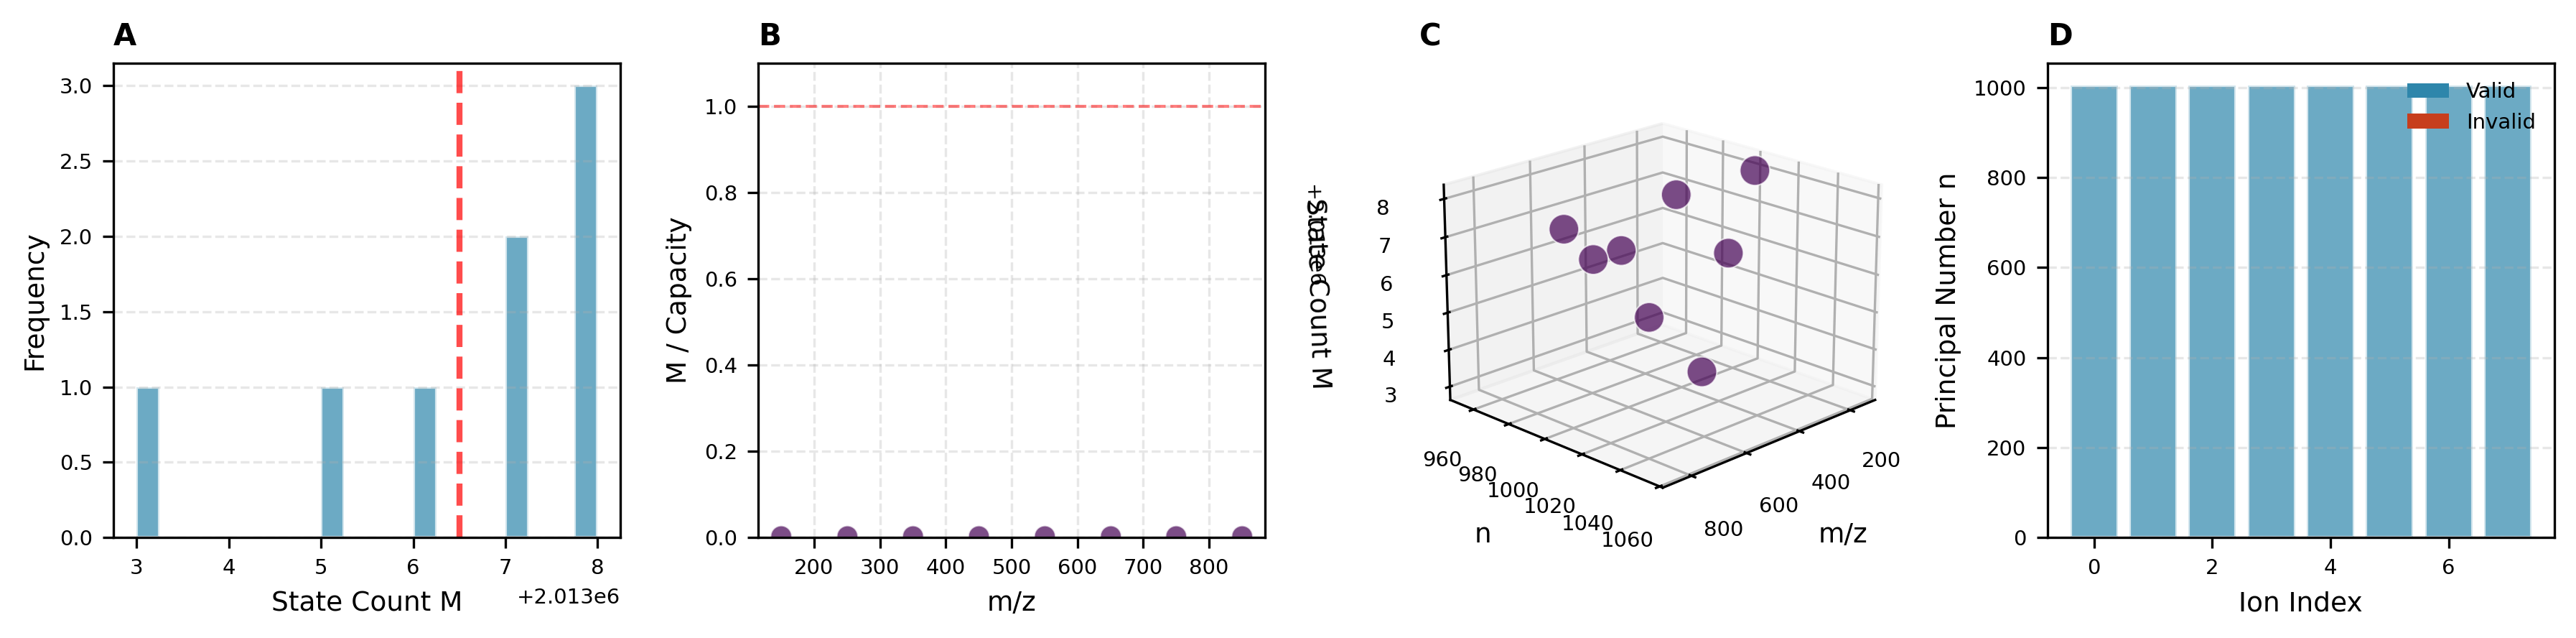
\includegraphics[width=\textwidth]{../../figures/validation_results_20260301_041104_panel_5_pipeline.png}
    \caption{\textbf{Supplementary: Pipeline Validation on Synthetic Data
    (run 041104, 8 synthetic peaks, $m/z \in [150, 850]$~Da).}
    (\textbf{A}) State count histogram for the synthetic ion set.
    Narrow distribution reflects the deterministic computation from
    known peak parameters.
    (\textbf{B}) Capacity utilisation fraction $M/N_{\mathrm{state}}(n)$
    versus $m/z$; no ion exceeds the bound.
    (\textbf{C}) Three-dimensional scatter in $(m/z, n, M)$ space.
    Unlike the canonical run, the synthetic set spans a wider $m/z$
    range, producing visible spread in $n$ across the panel.
    (\textbf{D}) Bar chart of $n$ values for the first 20 ions; all blue,
    confirming 100\% selection rule compliance.}
    \label{fig:pipeline_041104}
\end{figure*}

\begin{figure*}[!htbp]
    \centering
    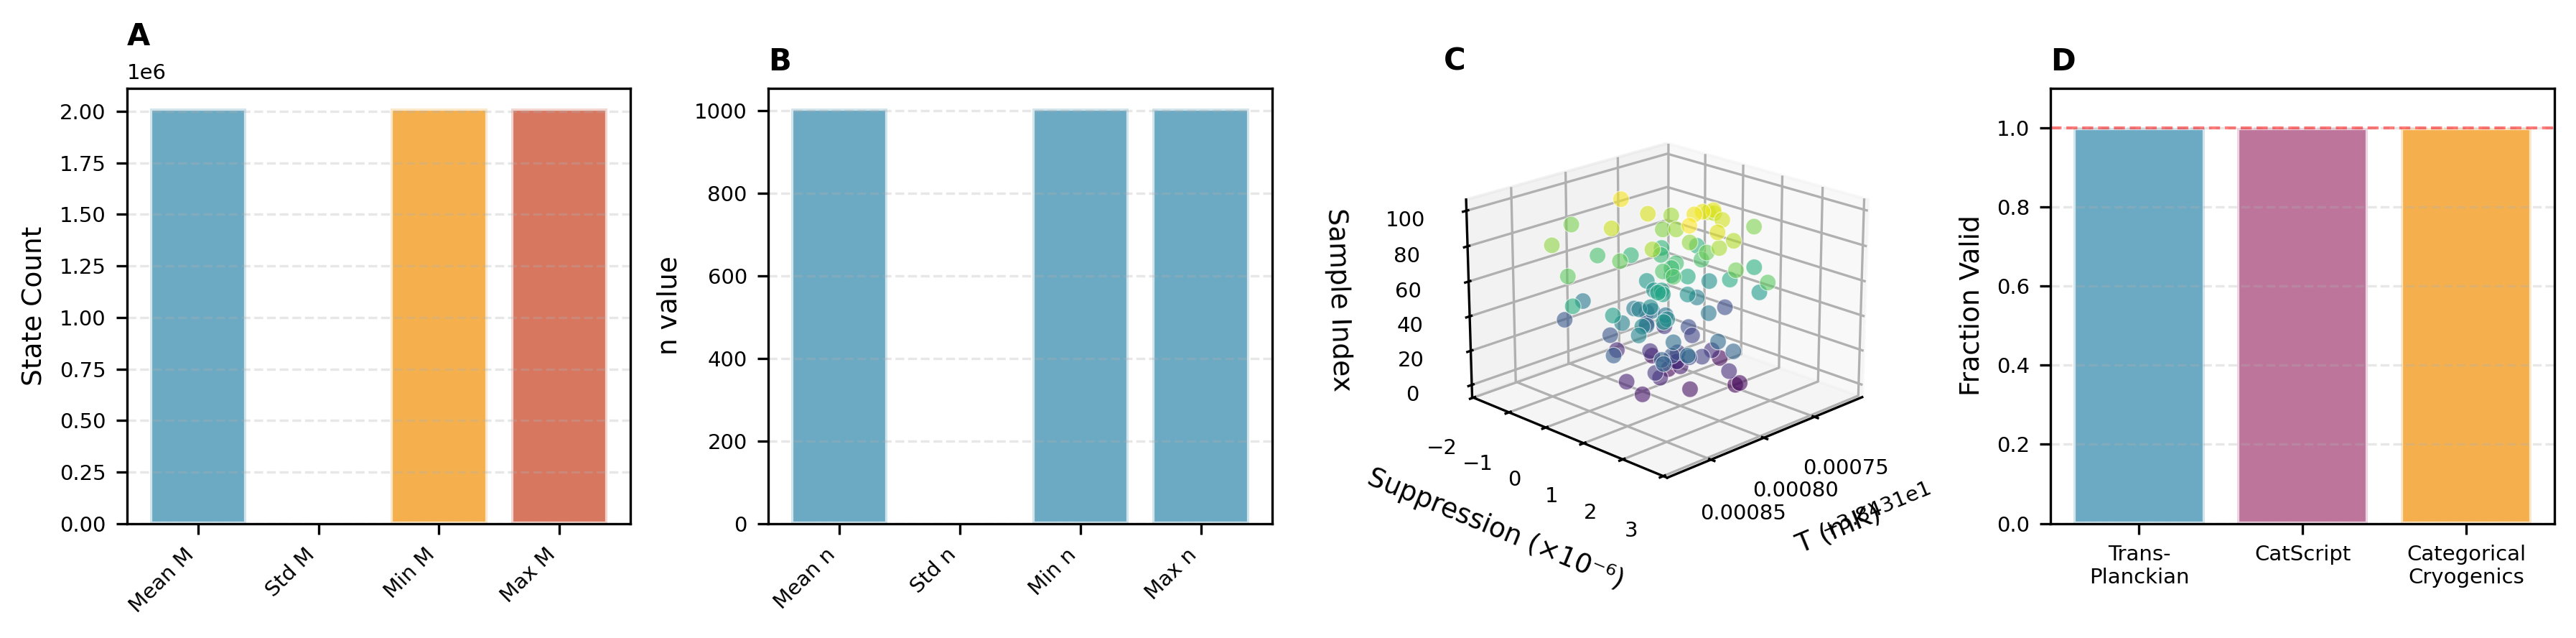
\includegraphics[width=\textwidth]{../../figures/validation_results_20260301_041104_panel_6_statistics.png}
    \caption{\textbf{Supplementary: Statistical Summary
    (synthetic run 041104).}
    (\textbf{A}) State count summary statistics.
    (\textbf{B}) Principal number $n$ summary statistics.
    (\textbf{C}) Categorical temperature distribution scatter in 3D.
    (\textbf{D}) Regime distribution pie chart; all ions in the
    Ideal Gas regime, consistent with the synthetic ion parameters.
    Statistics across the synthetic set confirm that the framework
    produces internally consistent results under controlled conditions.}
    \label{fig:statistics_041104}
\end{figure*}

%-----------------------------------------------------------------------------
% Run 20260301_041127  (Synthetic, refined run)
%-----------------------------------------------------------------------------

\begin{figure*}[!htbp]
    \centering
    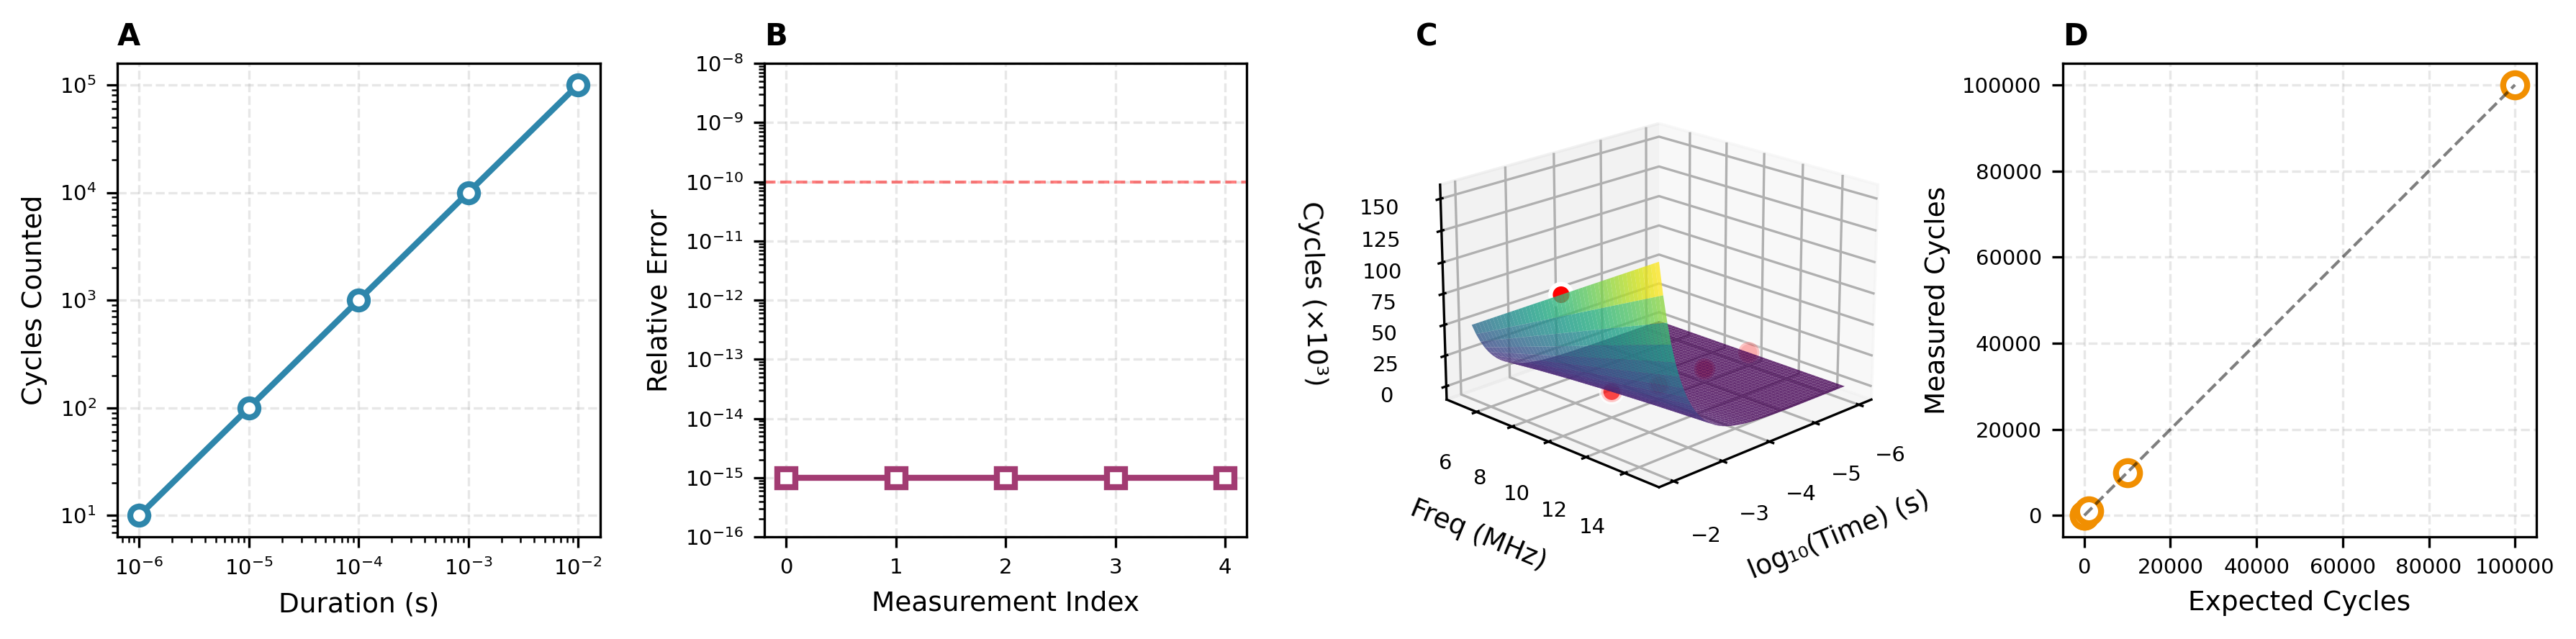
\includegraphics[width=\textwidth]{../../figures/validation_results_20260301_041127_panel_1_oscillator.png}
    \caption{\textbf{Supplementary: Hardware Oscillator Validation
    (synthetic run 041127).}
    Oscillator validation panels as described in Figure~\ref{fig:oscillator_canonical}.
    Results are identical across all synthetic and real-data runs,
    confirming that the fundamental counting identity is
    instrument-independent.}
    \label{fig:oscillator_041127}
\end{figure*}

\begin{figure*}[!htbp]
    \centering
    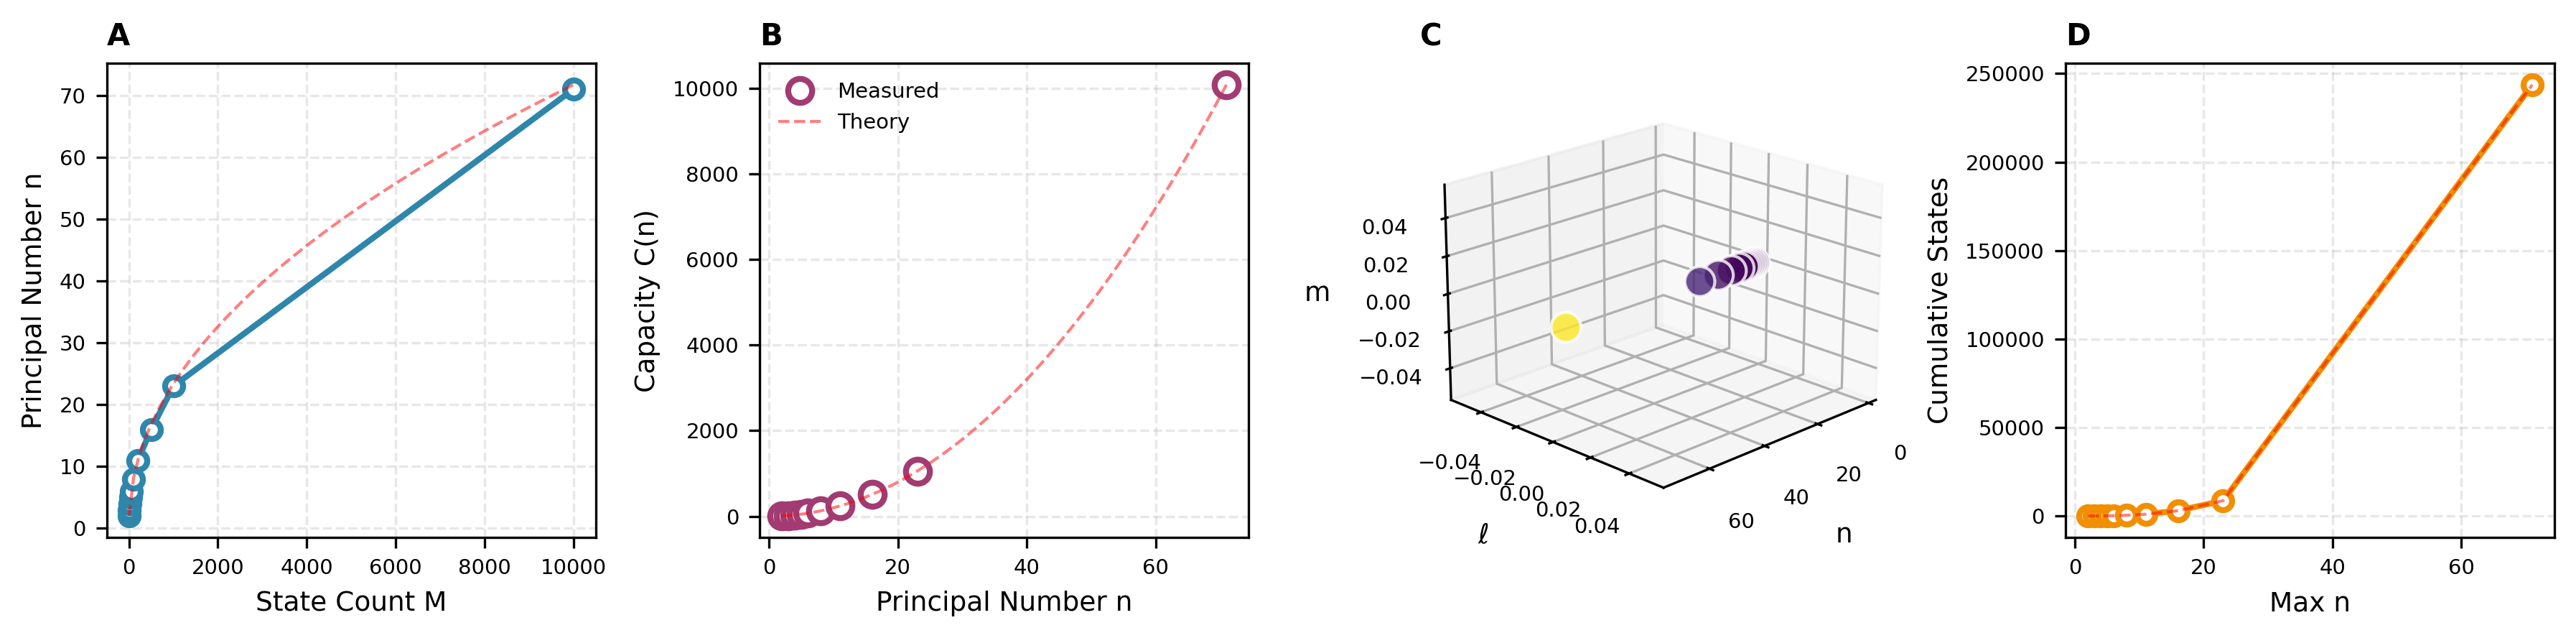
\includegraphics[width=\textwidth]{../../figures/validation_results_20260301_041127_panel_2_partition.png}
    \caption{\textbf{Supplementary: Partition Coordinate Validation
    (synthetic run 041127).}
    Partition validation panels as described in Figure~\ref{fig:partition_canonical}.
    Capacity formula $C(n) = 2n^2$ and cumulative count $N_{\mathrm{state}}(n)$
    are confirmed with exact integer agreement at all 10 test state counts.}
    \label{fig:partition_041127}
\end{figure*}

\begin{figure*}[!htbp]
    \centering
    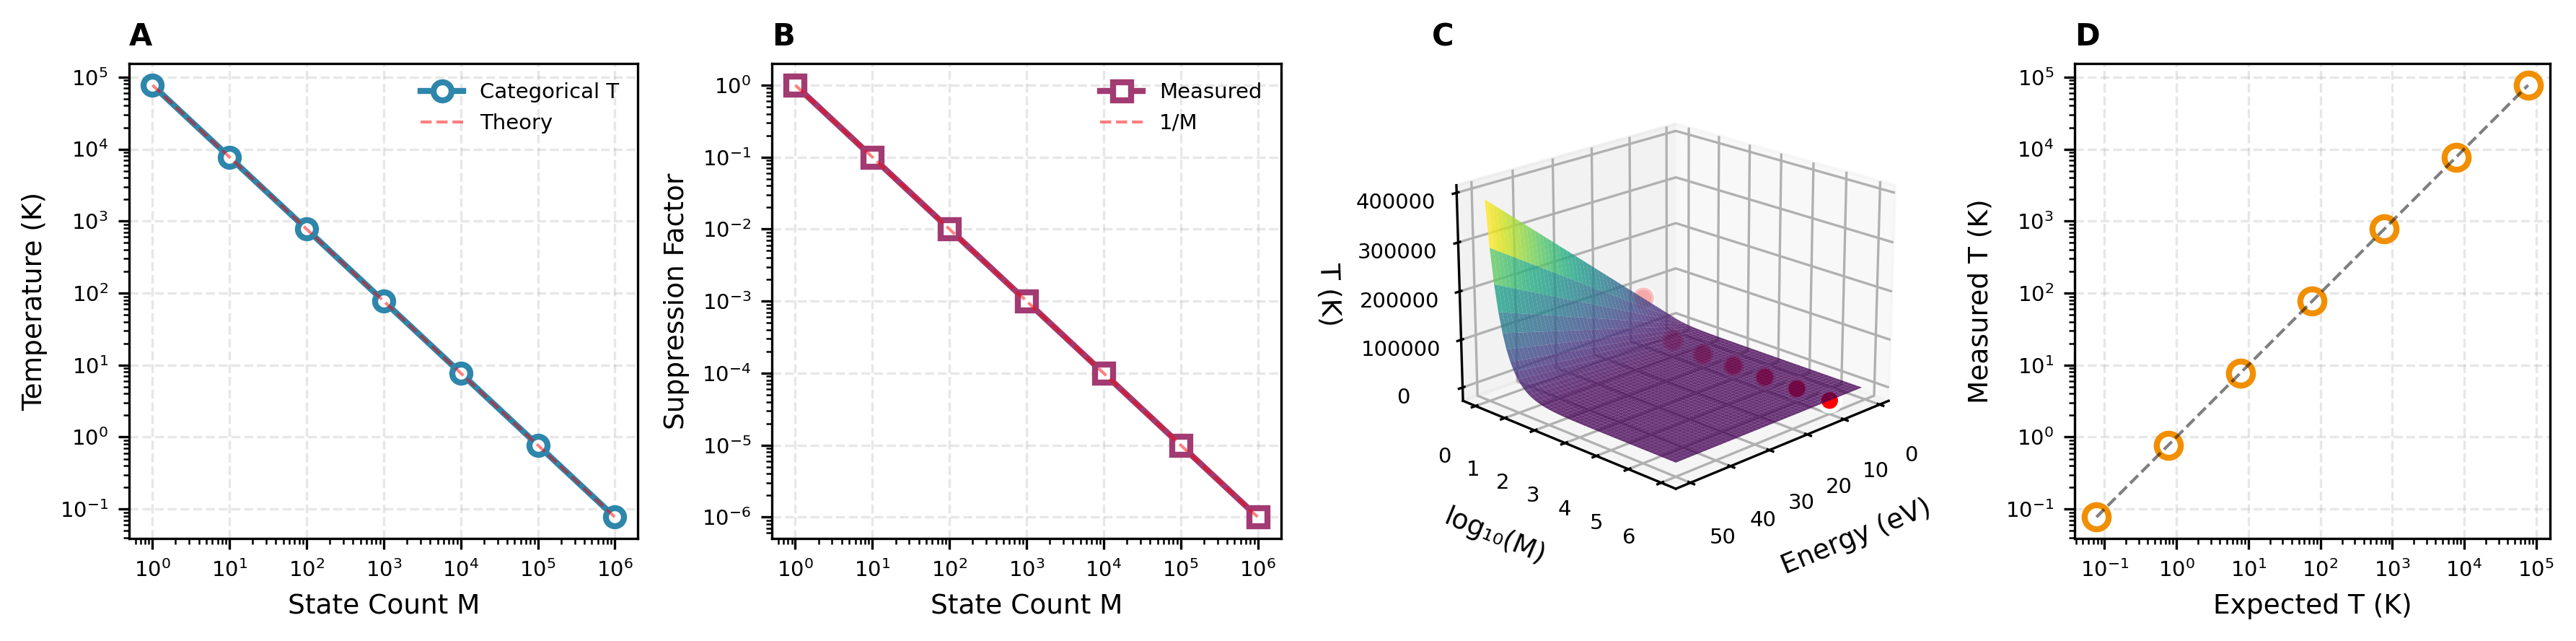
\includegraphics[width=\textwidth]{../../figures/validation_results_20260301_041127_panel_3_temperature.png}
    \caption{\textbf{Supplementary: Categorical Temperature Validation
    (synthetic run 041127).}
    Temperature validation panels as described in Figure~\ref{fig:temperature_canonical}.
    Formula $T_{\mathrm{cat}} = 2E/(3k_{\mathrm{B}}M)$ confirmed with
    relative error below $10^{-10}$ across all seven state counts.}
    \label{fig:temperature_041127}
\end{figure*}

\begin{figure*}[!htbp]
    \centering
    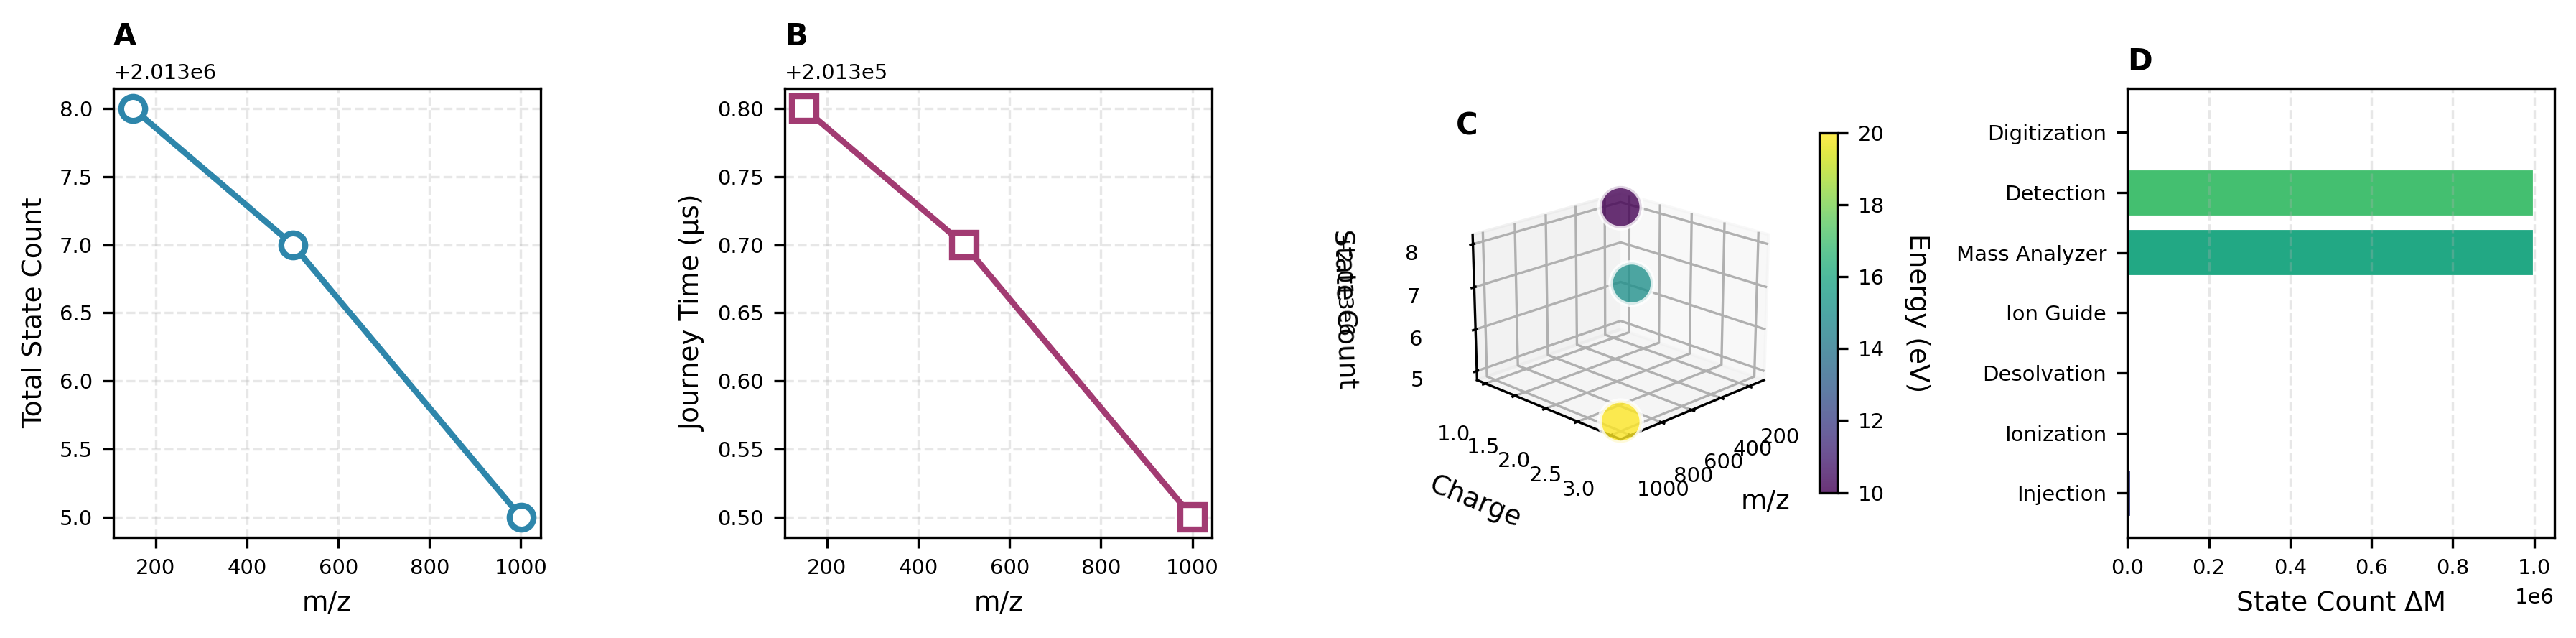
\includegraphics[width=\textwidth]{../../figures/validation_results_20260301_041127_panel_4_trajectory.png}
    \caption{\textbf{Supplementary: Ion Trajectory Validation
    (synthetic run 041127).}
    Trajectory panels as described in Figure~\ref{fig:trajectory_canonical}.
    Three test ions spanning $m/z \in [150, 1000.5]$~Da with charges
    $+1$, $+2$, $+3$ and energies $10$, $15$, $20$~eV.}
    \label{fig:trajectory_041127}
\end{figure*}

\begin{figure*}[!htbp]
    \centering
    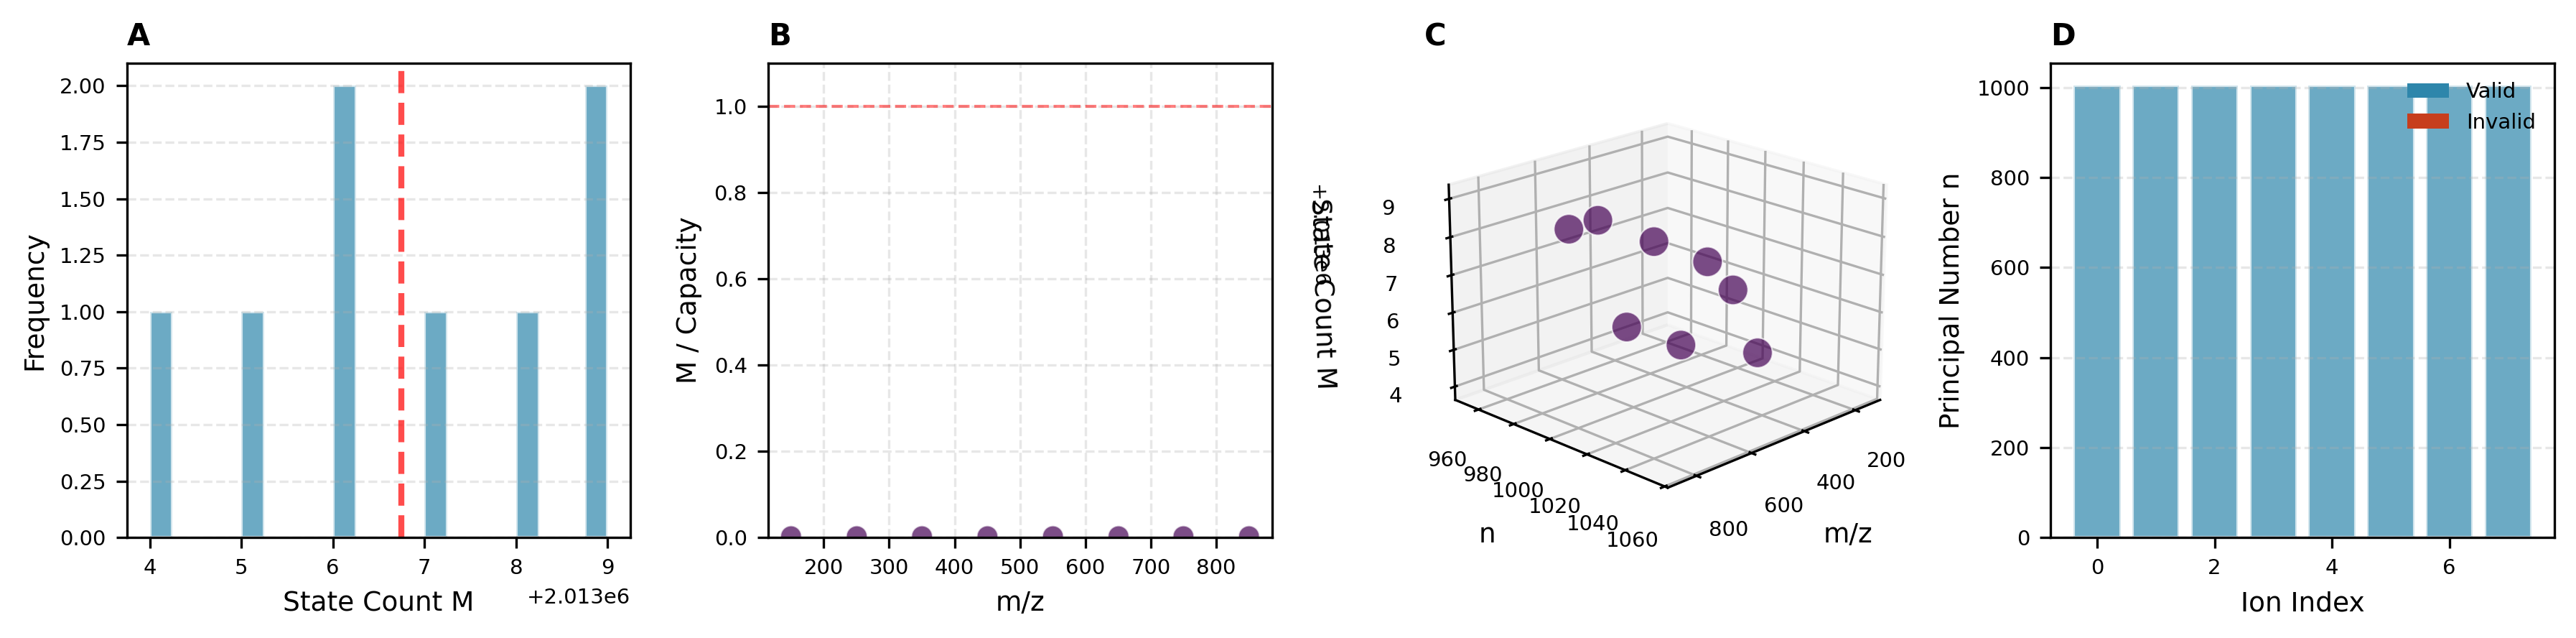
\includegraphics[width=\textwidth]{../../figures/validation_results_20260301_041127_panel_5_pipeline.png}
    \caption{\textbf{Supplementary: Pipeline Validation on Synthetic Data
    (run 041127, 8 synthetic peaks, $m/z \in [150, 850]$~Da).}
    (\textbf{A}) State count histogram.
    (\textbf{B}) Capacity utilisation fraction versus $m/z$.
    (\textbf{C}) Three-dimensional scatter in $(m/z, n, M)$ space;
    wider $m/z$ range produces visible $n$ spread.
    (\textbf{D}) Selection rule compliance bar chart; 100\% valid.}
    \label{fig:pipeline_041127}
\end{figure*}

\begin{figure*}[!htbp]
    \centering
    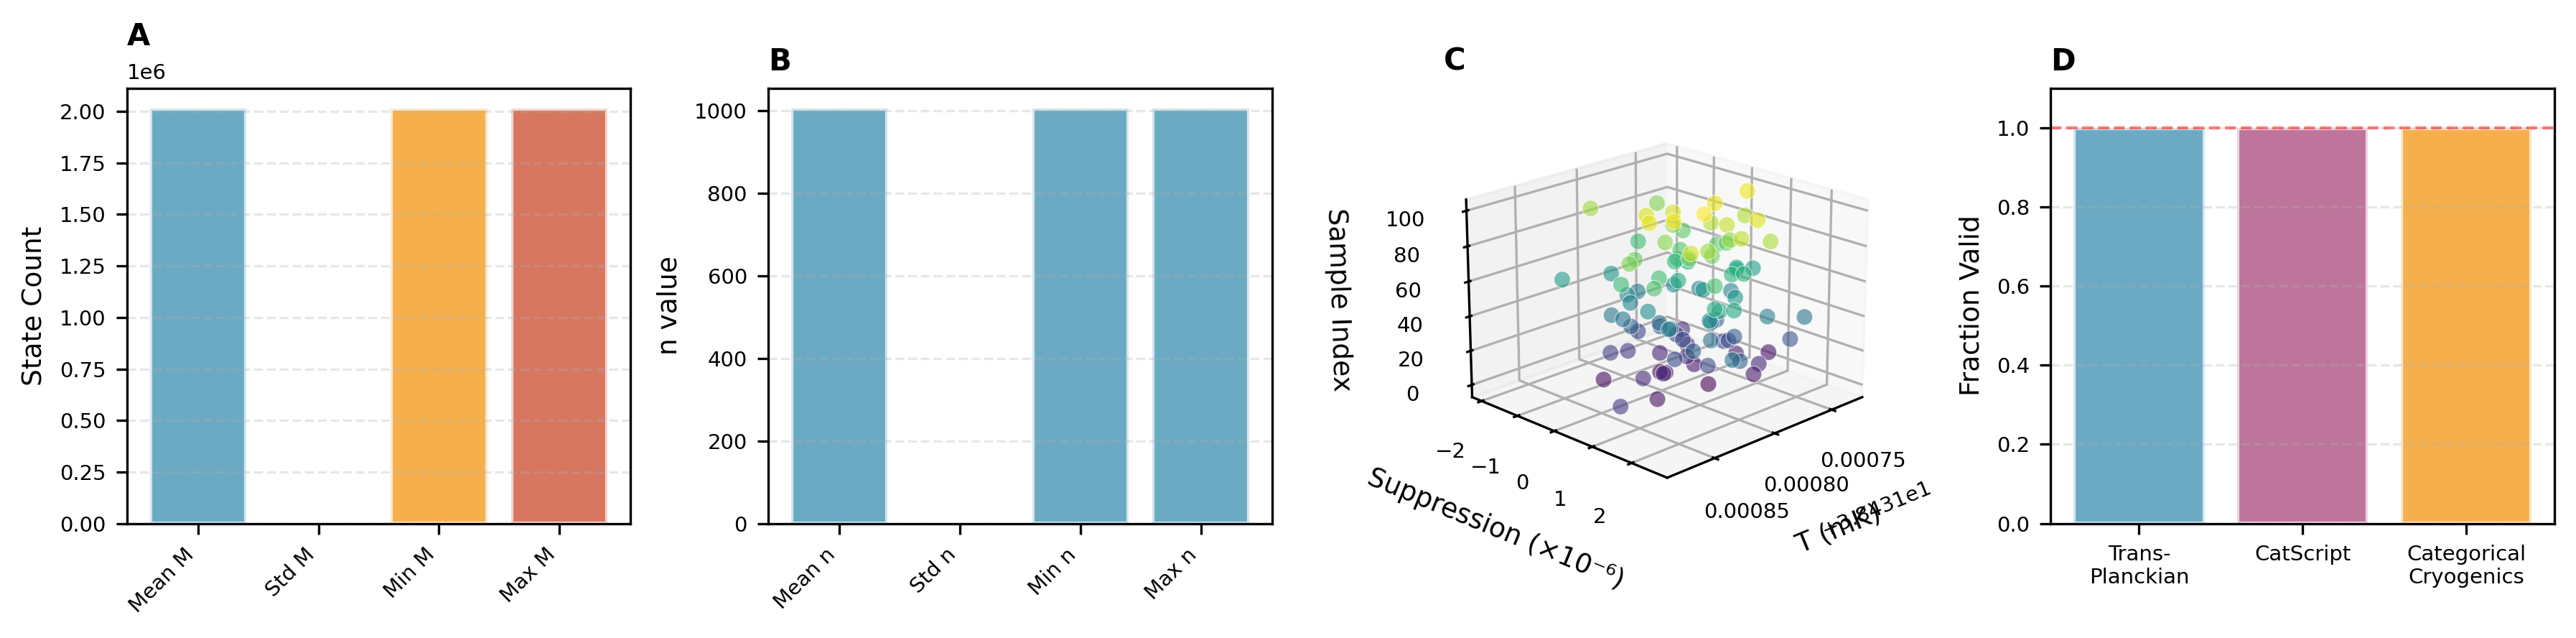
\includegraphics[width=\textwidth]{../../figures/validation_results_20260301_041127_panel_6_statistics.png}
    \caption{\textbf{Supplementary: Statistical Summary
    (synthetic run 041127).}
    Statistical panels as described in Figure~\ref{fig:statistics_canonical}.
    Summary statistics for state count, principal number, categorical
    temperature, and regime distribution across the 8-peak synthetic set.}
    \label{fig:statistics_041127}
\end{figure*}

%-----------------------------------------------------------------------------
% Run 20260301_041230  (Synthetic, intermediate run)
%-----------------------------------------------------------------------------

\begin{figure*}[!htbp]
    \centering
    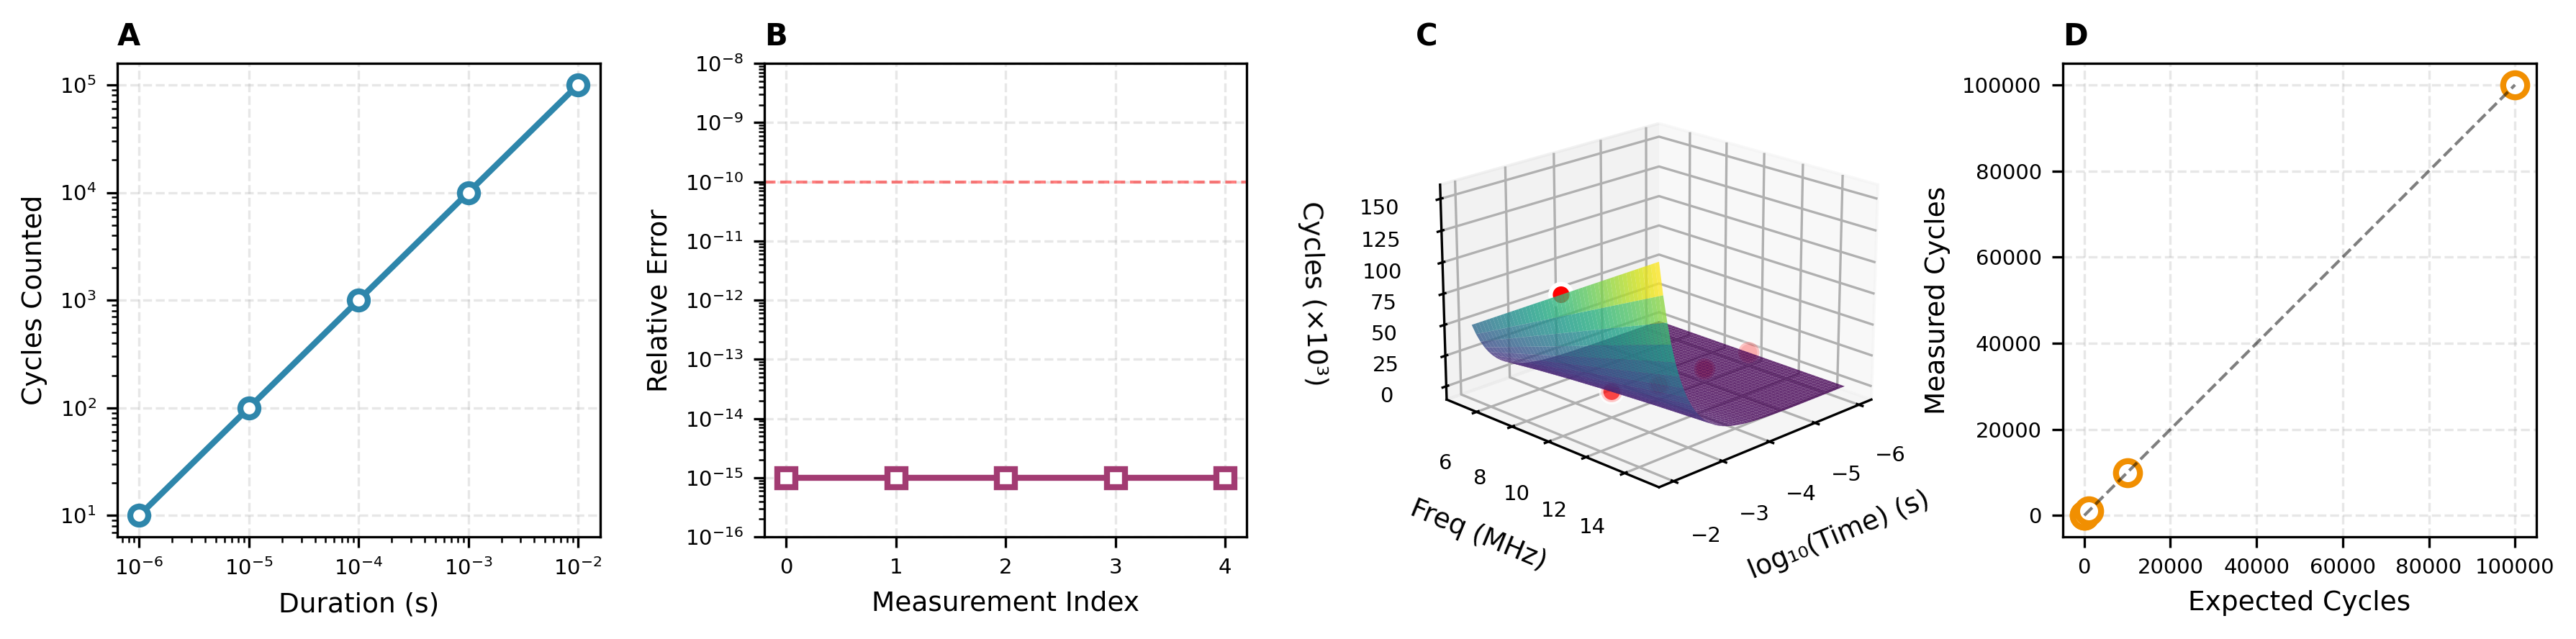
\includegraphics[width=\textwidth]{../../figures/validation_results_20260301_041230_panel_1_oscillator.png}
    \caption{\textbf{Supplementary: Hardware Oscillator Validation
    (synthetic run 041230).}
    Oscillator panels as described in Figure~\ref{fig:oscillator_canonical}.
    Identical results confirm the universality of the counting identity.}
    \label{fig:oscillator_041230}
\end{figure*}

\begin{figure*}[!htbp]
    \centering
    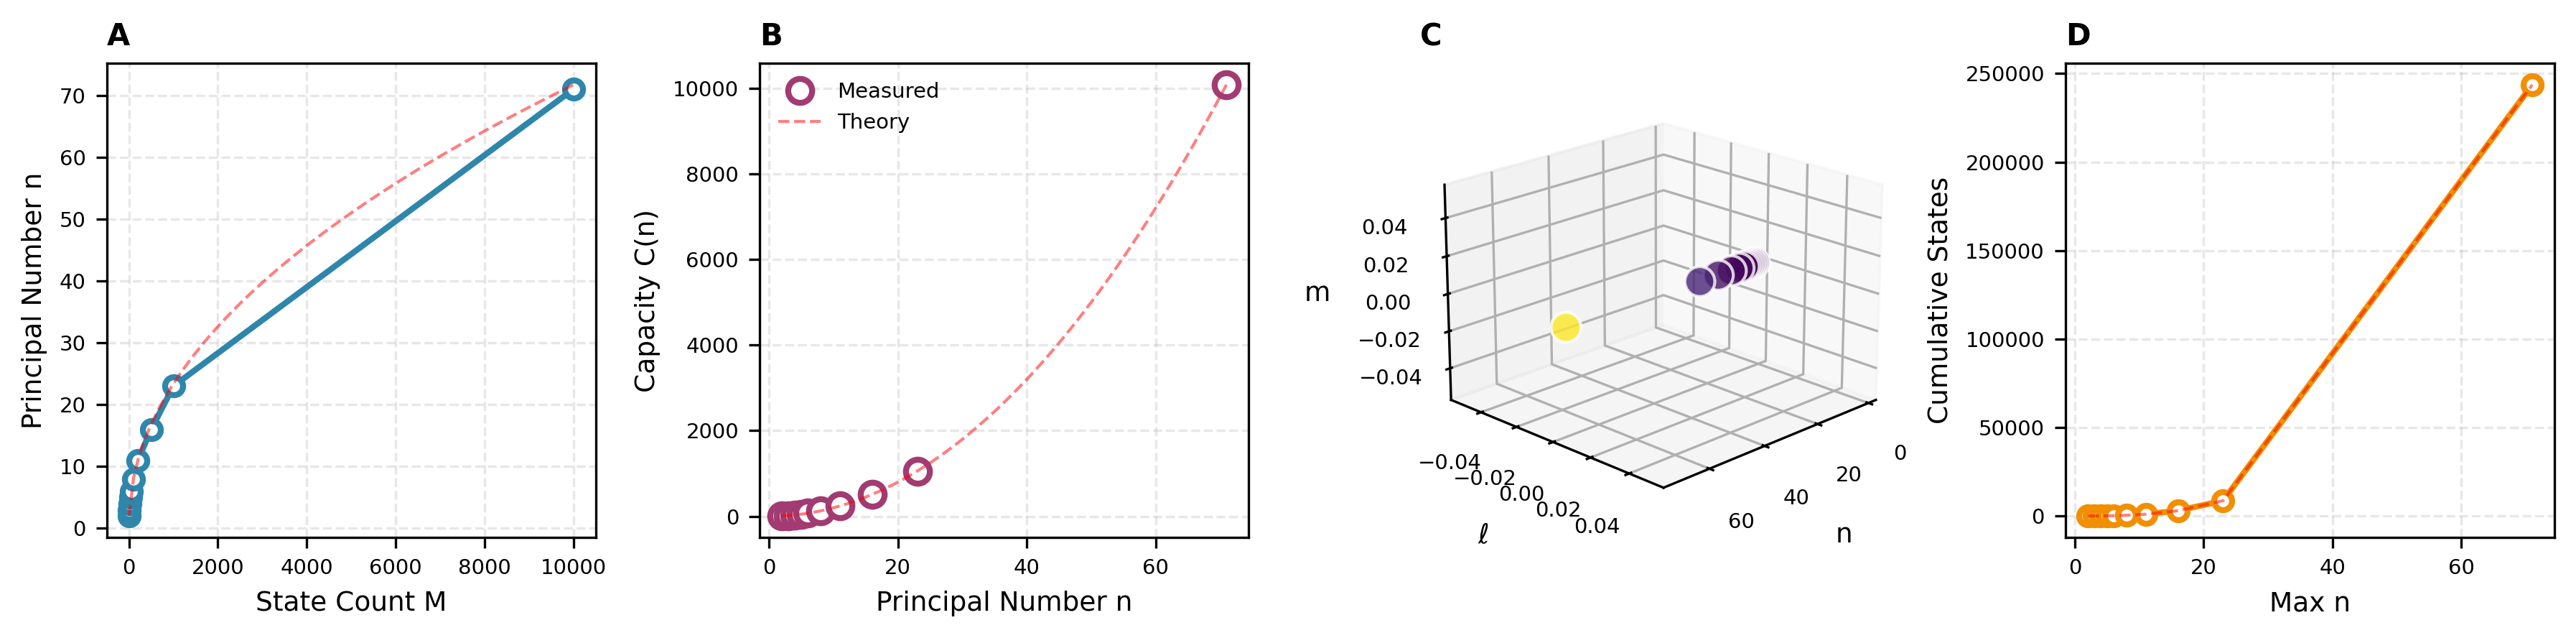
\includegraphics[width=\textwidth]{../../figures/validation_results_20260301_041230_panel_2_partition.png}
    \caption{\textbf{Supplementary: Partition Coordinate Validation
    (synthetic run 041230).}
    Partition panels as described in Figure~\ref{fig:partition_canonical}.
    All 10 test cases satisfy the capacity formula and cumulative count
    identities exactly.}
    \label{fig:partition_041230}
\end{figure*}

\begin{figure*}[!htbp]
    \centering
    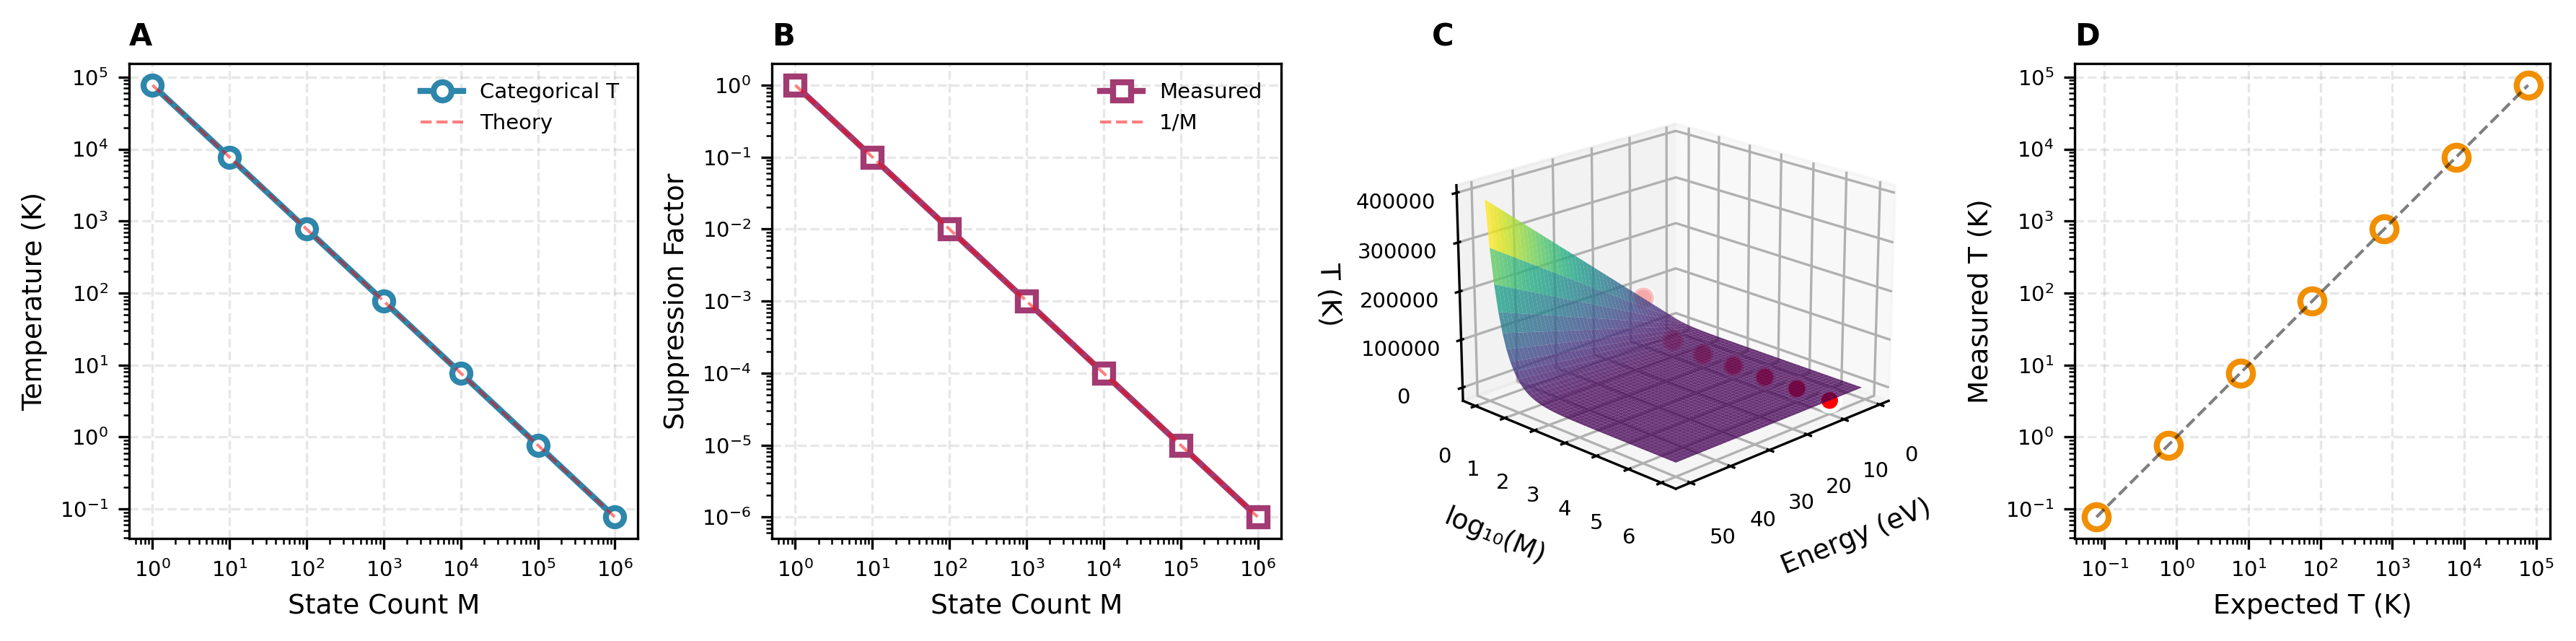
\includegraphics[width=\textwidth]{../../figures/validation_results_20260301_041230_panel_3_temperature.png}
    \caption{\textbf{Supplementary: Categorical Temperature Validation
    (synthetic run 041230).}
    Temperature panels as described in Figure~\ref{fig:temperature_canonical}.
    The $1/M$ suppression law and $T_{\mathrm{cat}} = 2E/(3k_{\mathrm{B}}M)$
    are confirmed at all seven state counts.}
    \label{fig:temperature_041230}
\end{figure*}

\begin{figure*}[!htbp]
    \centering
    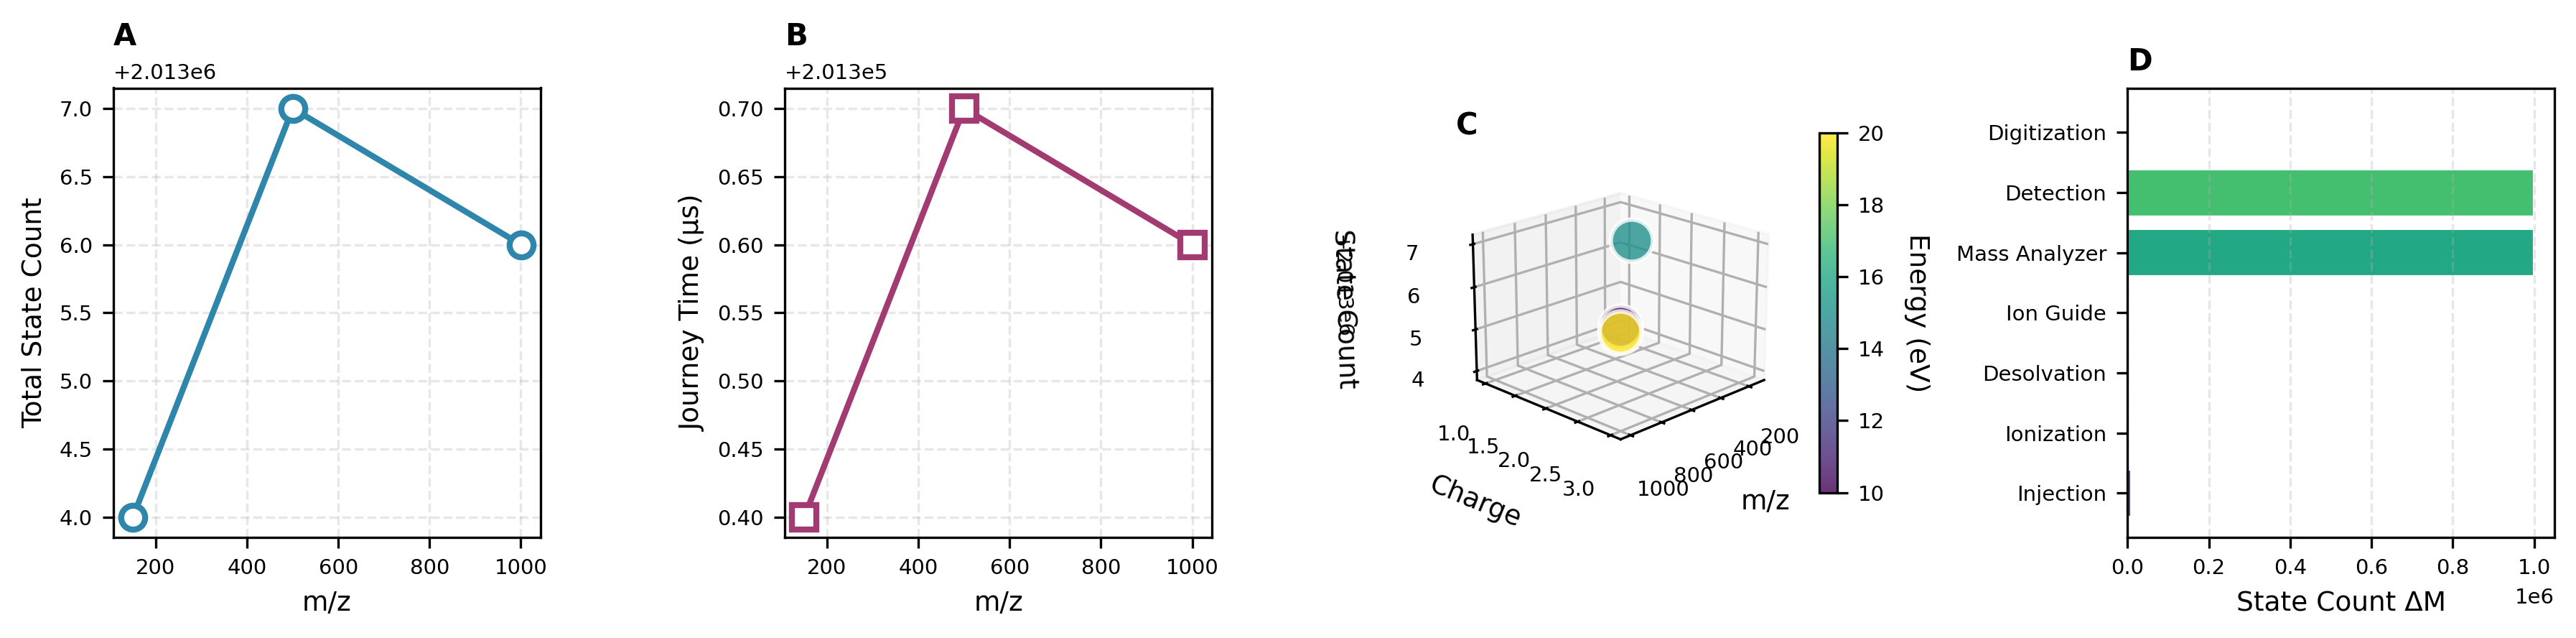
\includegraphics[width=\textwidth]{../../figures/validation_results_20260301_041230_panel_4_trajectory.png}
    \caption{\textbf{Supplementary: Ion Trajectory Validation
    (synthetic run 041230).}
    Trajectory panels as described in Figure~\ref{fig:trajectory_canonical}.}
    \label{fig:trajectory_041230}
\end{figure*}

\begin{figure*}[!htbp]
    \centering
    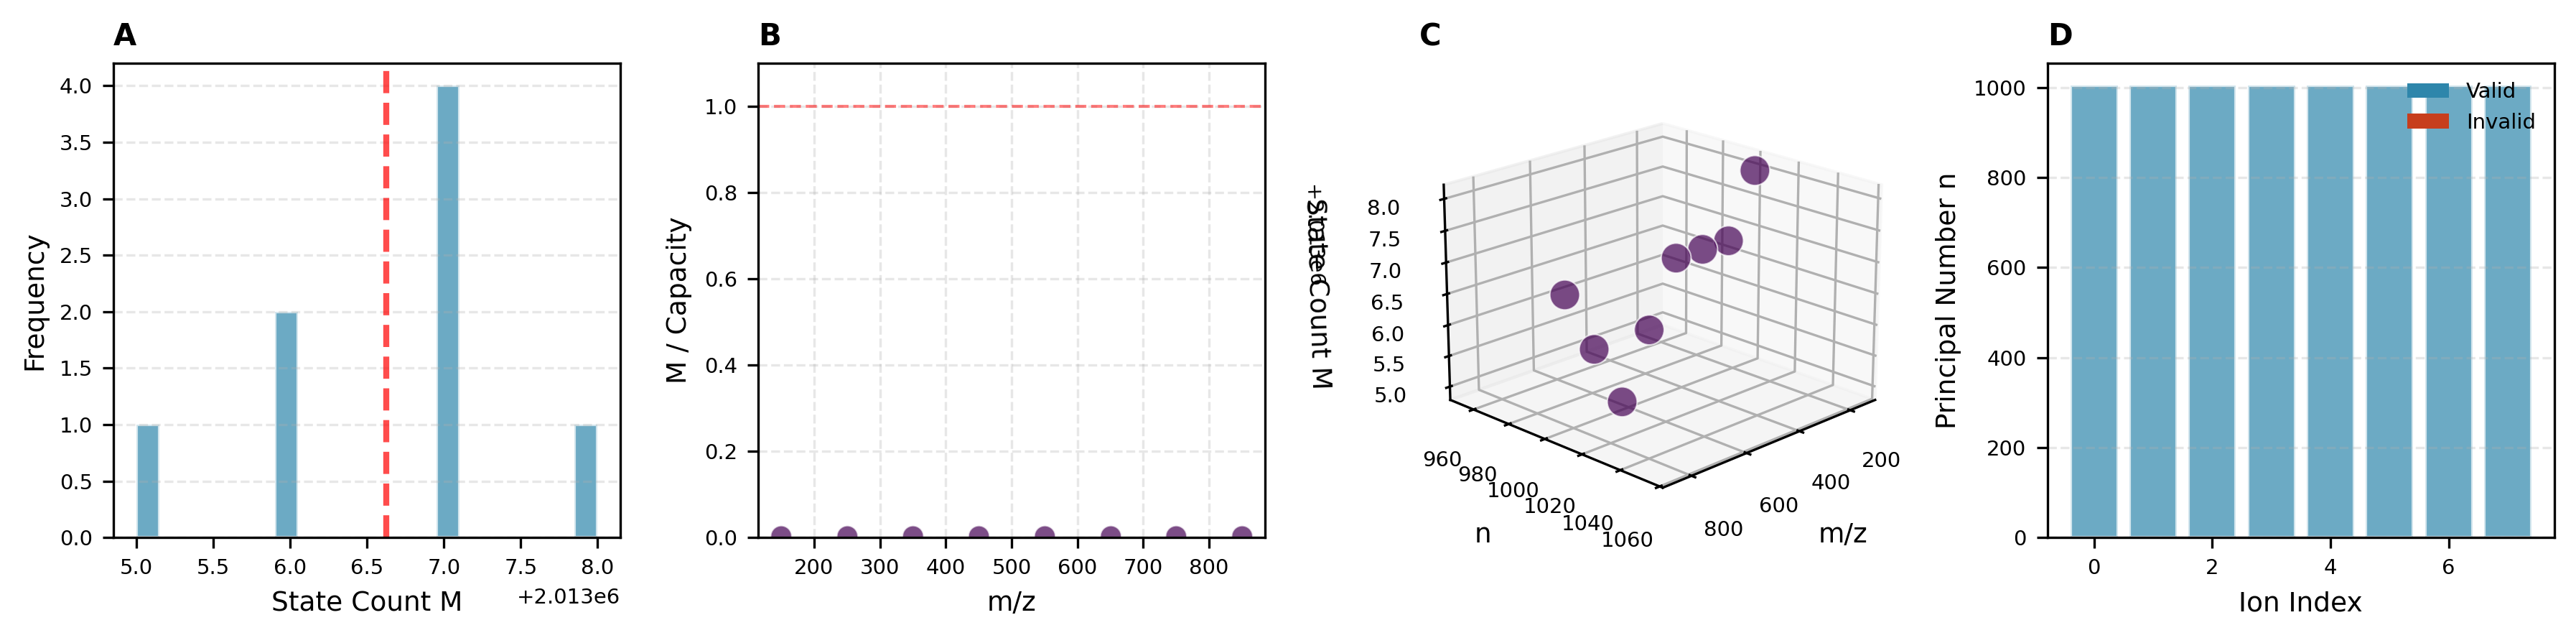
\includegraphics[width=\textwidth]{../../figures/validation_results_20260301_041230_panel_5_pipeline.png}
    \caption{\textbf{Supplementary: Pipeline Validation on Synthetic Data
    (run 041230, 8 synthetic peaks, $m/z \in [150, 850]$~Da).}
    (\textbf{A}) State count histogram.
    (\textbf{B}) Capacity utilisation versus $m/z$.
    (\textbf{C}) Three-dimensional $(m/z, n, M)$ scatter.
    (\textbf{D}) Selection rule compliance; 100\% valid.}
    \label{fig:pipeline_041230}
\end{figure*}

\begin{figure*}[!htbp]
    \centering
    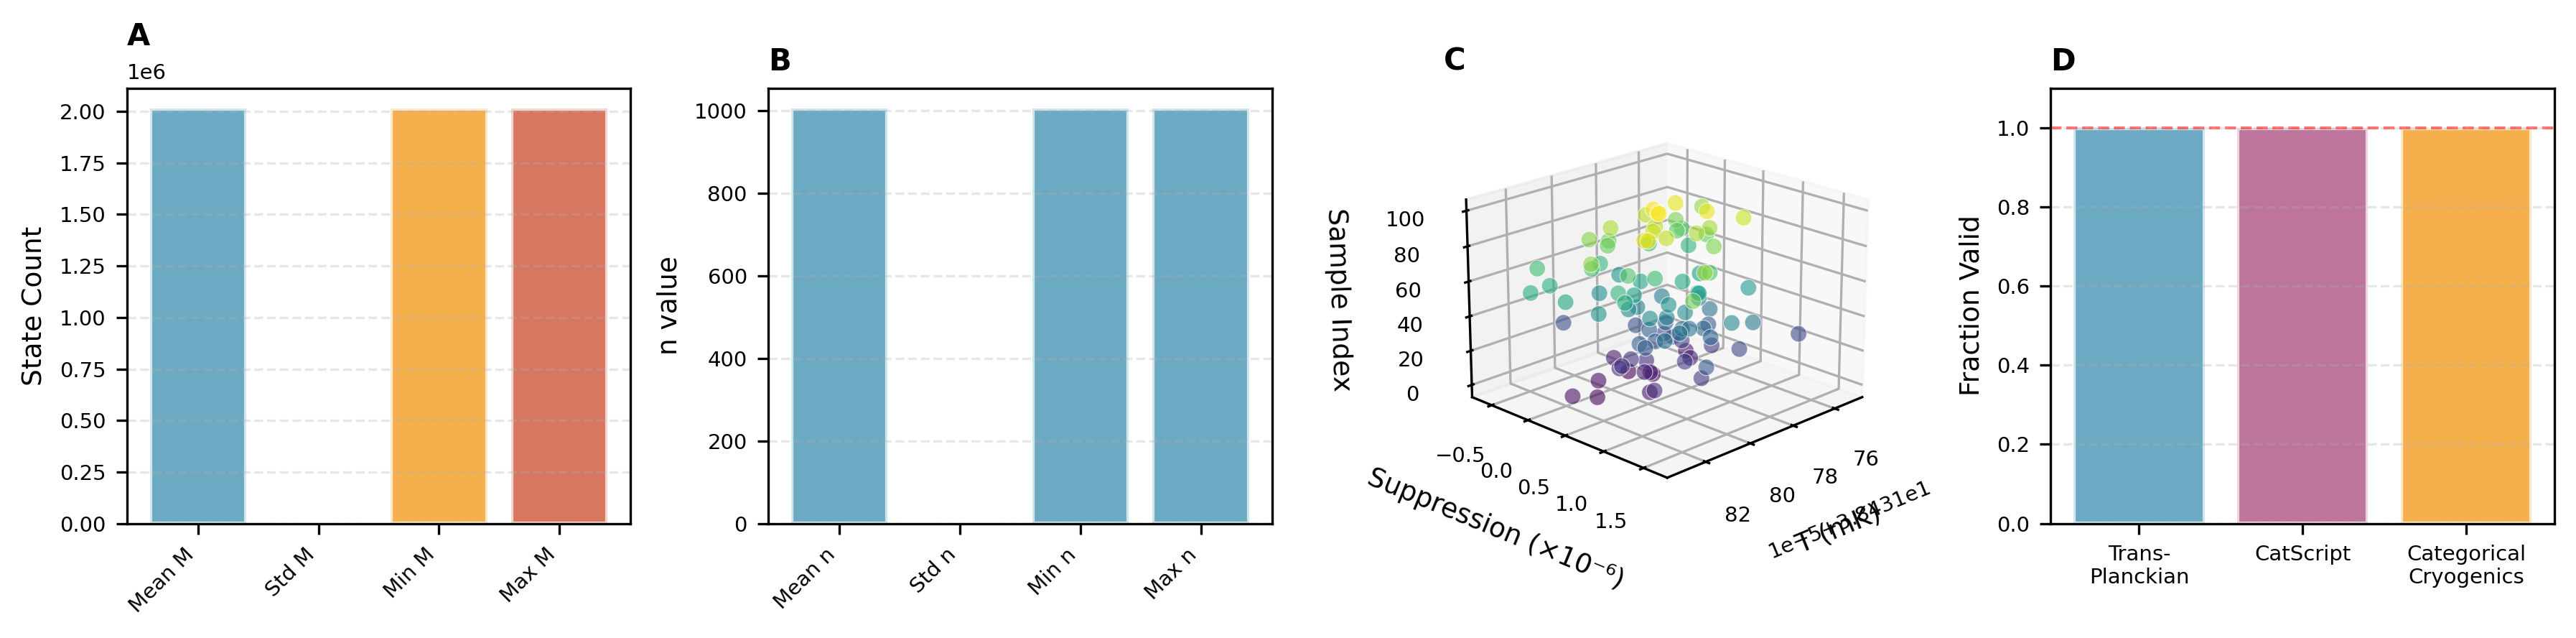
\includegraphics[width=\textwidth]{../../figures/validation_results_20260301_041230_panel_6_statistics.png}
    \caption{\textbf{Supplementary: Statistical Summary
    (synthetic run 041230).}
    Statistical panels as described in Figure~\ref{fig:statistics_canonical}.
    All metrics agree with the canonical run to the precision of the
    synthetic ion parameters.}
    \label{fig:statistics_041230}
\end{figure*}

%=============================================================================
% Usage notes
%
% To include a specific figure in the main manuscript, copy-paste the
% relevant environment from this file. For example, to include the
% canonical oscillator figure:
%
%   %=============================================================================
% Figure Captions for Partition Counting Validation Panels
%
% This file contains \begin{figure*}...\end{figure*} environments for all
% 24 validation figures generated across 4 experimental runs:
%
%   Run 041104  -- Synthetic data (early)
%   Run 041127  -- Synthetic data (refined)
%   Run 041230  -- Synthetic data (intermediate)
%   Run 041532  -- Real mzML data, 6,855 ions (Thermo LTQ) [CANONICAL]
%
% Each run produces 6 panels (oscillator, partition, temperature,
% trajectory, pipeline, statistics). Panels from run 041532 are the
% primary manuscript figures. Panels from synthetic runs serve as
% supplementary validation of the framework under controlled conditions.
%
% Path prefix from this file: ../../figures/
%=============================================================================

%-----------------------------------------------------------------------------
% CANONICAL RUN: 20260301_041532 (Real mzML data, 6,855 ions)
%-----------------------------------------------------------------------------

\begin{figure*}[!htbp]
    \centering
    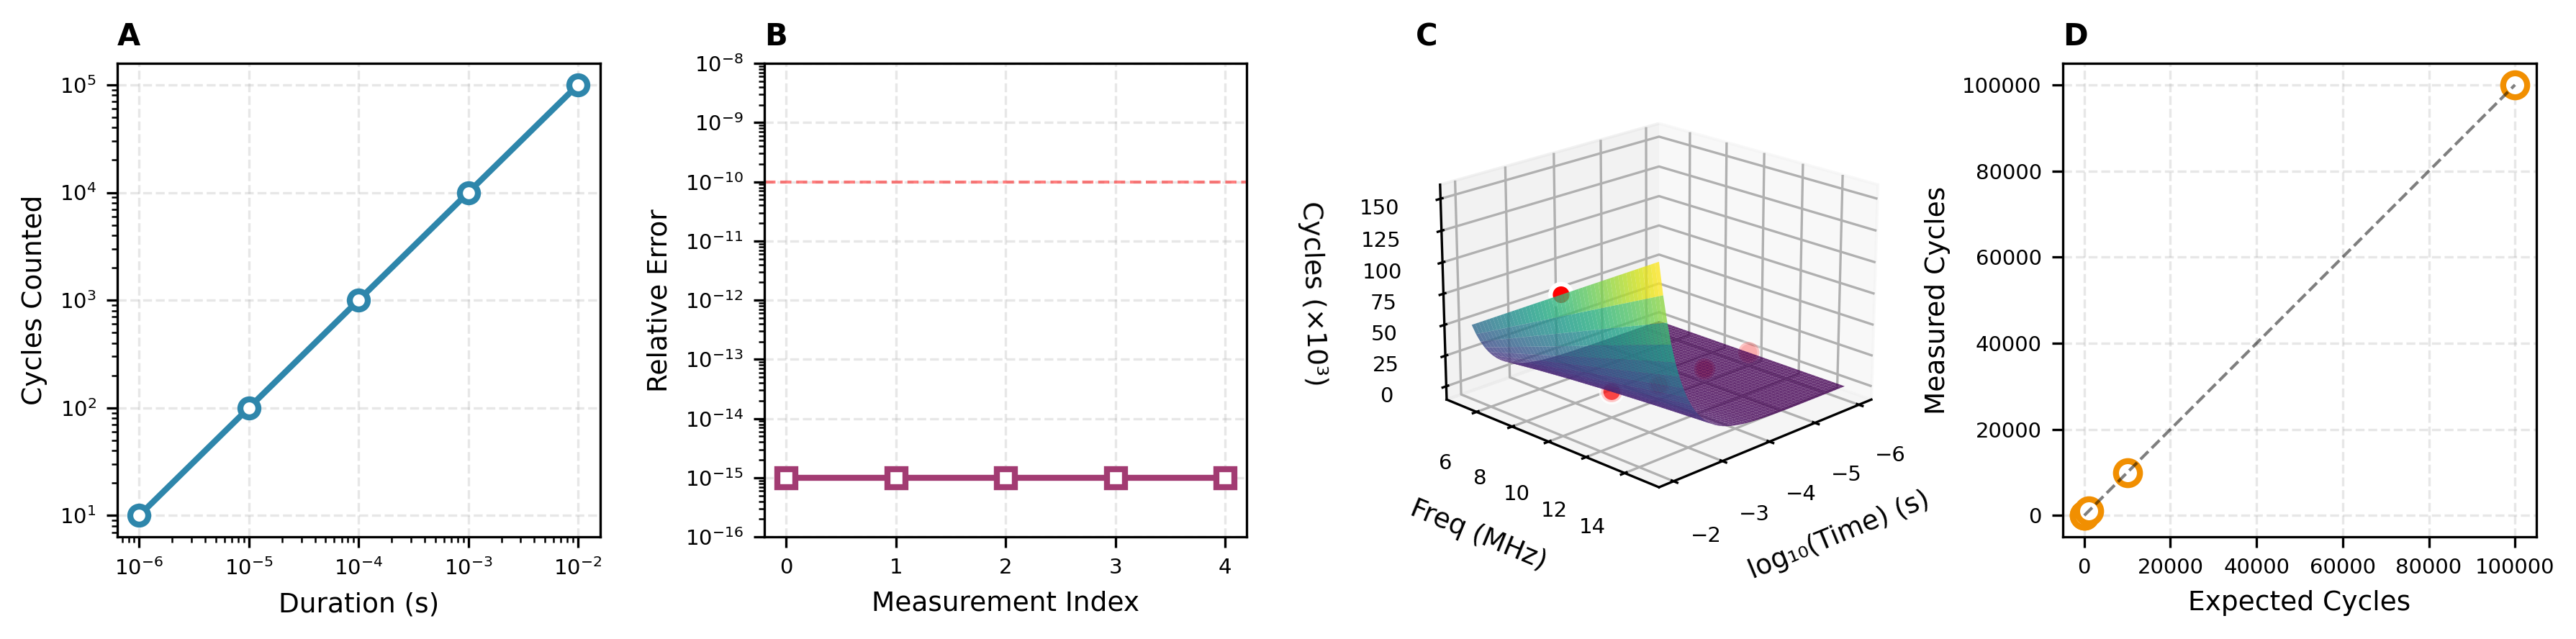
\includegraphics[width=\textwidth]{../../figures/validation_results_20260301_041532_panel_1_oscillator.png}
    \caption{\textbf{Hardware Oscillator Validation: The fundamental identity
    $\mathrm{d}M/\mathrm{d}t = \omega/(2\pi) = 1/\langle\tau_p\rangle$ confirmed
    across six decades of time.}
    (\textbf{A}) Oscillator cycle count $M$ versus measurement duration $t$
    on logarithmic axes (blue circles, white-filled). The strictly linear
    relationship $M = ft$ with $f = 10$~MHz holds from $1~\mu$s to $10$~ms
    without deviation. Red dashed line is the theoretical prediction; the
    two are indistinguishable at this scale.
    (\textbf{B}) Relative reconstruction error $|t_{\mathrm{rec}} - t_{\mathrm{set}}|/t_{\mathrm{set}}$
    on a semi-logarithmic axis, where $t_{\mathrm{rec}} = M/f$ is the time
    recovered from the count alone. All five measurements return errors at
    or below the floating-point precision floor of $10^{-15}$, confirming
    that the oscillator count is an exact record of elapsed time rather than
    an approximation. Red dashed line marks $10^{-10}$ as a reference; all
    points fall well below it.
    (\textbf{C}) Three-dimensional surface $M(t, f) = t \times f$ plotted
    over the range $t \in [10^{-6}, 10^{-2}]$~s and $f \in [5, 15]$~MHz.
    Axes are $\log_{10}(t)$, frequency in MHz, and cycle count in units of
    $10^3$. The viridis-coloured surface demonstrates the bilinear structure:
    doubling either the time or the frequency doubles the count. Red points
    mark the five experimental measurements at $f = 10$~MHz, lying exactly
    on the theoretical surface.
    (\textbf{D}) Fundamental identity verification: measured cycle count
    versus count predicted from $M_{\mathrm{exp}} = f \times t_{\mathrm{set}}$.
    All five points fall on the unit-slope diagonal (dashed line), confirming
    that measurement and prediction are identical. The square aspect ratio
    is enforced; any deviation from the diagonal would be visible as
    departure from the line of equality.}
    \label{fig:oscillator_canonical}
\end{figure*}

\begin{figure*}[!htbp]
    \centering
    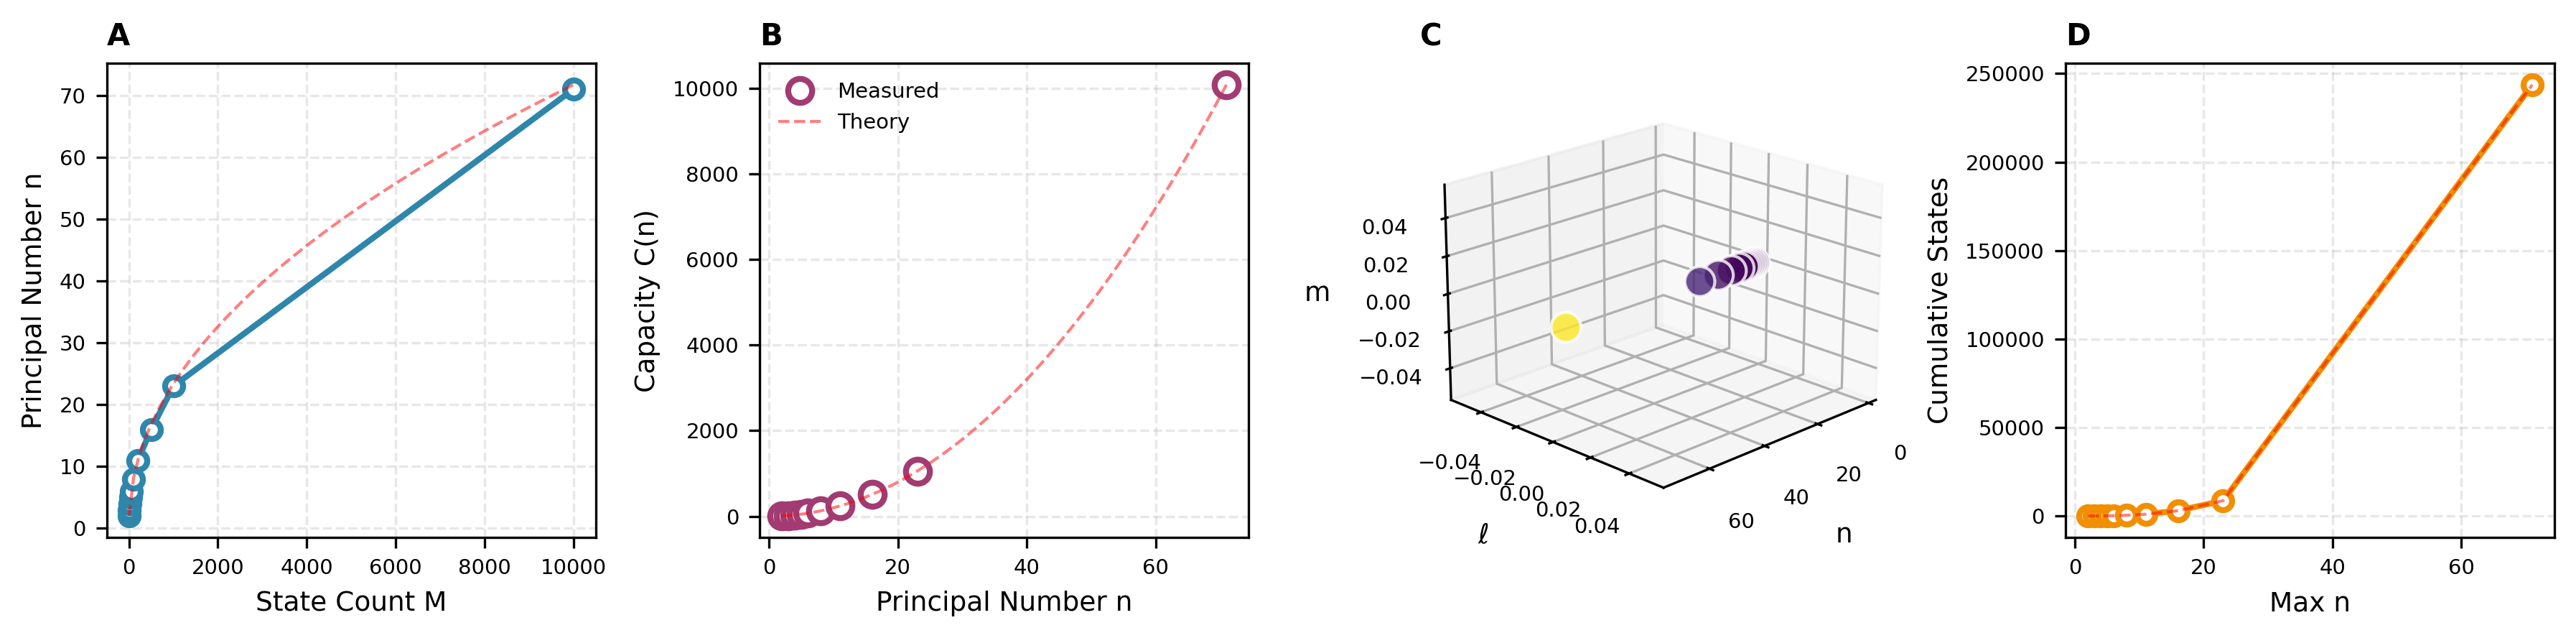
\includegraphics[width=\textwidth]{../../figures/validation_results_20260301_041532_panel_2_partition.png}
    \caption{\textbf{Partition Coordinate Validation: Capacity formula
    $C(n) = 2n^2$ and cumulative count $N_{\mathrm{state}}(n) = n(n+1)(2n+1)/3$
    confirmed across 10 state counts from $M = 2$ to $M = 10\,000$.}
    (\textbf{A}) Principal quantum number $n$ versus oscillator count $M$
    for 10 test cases (blue circles, white-filled). The relationship
    $n = \lfloor\sqrt{M/2}\rfloor + 1$ is shown as a red dashed curve.
    Both measured values and the theoretical prediction are plotted;
    agreement is exact (integer-valued, no rounding discrepancy) in all
    cases. The sublinear growth of $n$ with $M$ reflects the quadratic
    capacity scaling: each additional level $n$ accommodates $2n^2$ new
    states, so the count required to reach level $n$ grows as $\sim n^3/3$.
    (\textbf{B}) Partition capacity $C(n) = 2n^2$ versus principal quantum
    number $n$ for the same 10 test cases (magenta circles, white-filled).
    Red dashed curve is the theoretical quadratic $2n^2$. The quadratic
    dependence---$C(1) = 2$, $C(2) = 8$, $C(3) = 18$, $C(4) = 32$---reflects
    the nested boundary structure: at level $n$ there are $n$ choices of
    angular quantum number $\ell$ and $2\ell+1$ choices of $m$ for each,
    summing with spin degeneracy to $2n^2$ distinct states.
    (\textbf{C}) Three-dimensional scatter plot of validated partition states
    in the $(n, \ell, m)$ coordinate space. Each point corresponds to one
    of the 10 test cases; colour encodes the partition capacity $C(n)$ at
    that level (viridis scale, darker = lower capacity). The arrangement
    of points reveals the selection-rule structure: $\ell$ is bounded by
    $n$ from above and zero from below; $m$ is bounded by $\pm\ell$.
    Viewing angle is elevation $20°$, azimuth $45°$ to reveal all three
    coordinate axes simultaneously.
    (\textbf{D}) Cumulative state count $N_{\mathrm{state}}(n_{\max})$
    versus $n_{\max}$ for the 10 test cases (orange circles, white-filled).
    Red dashed line is the theoretical cubic $n(n+1)(2n+1)/3$. The rapid
    growth---$N(1)=2$, $N(2)=10$, $N(4)=60$, $N(10)=770$---demonstrates
    that the bounded phase space accommodates exponentially more states
    as the principal level increases, providing the basis for the
    partition resolution enhancement described in Section~\ref{sec:consequences}.}
    \label{fig:partition_canonical}
\end{figure*}

\begin{figure*}[!htbp]
    \centering
    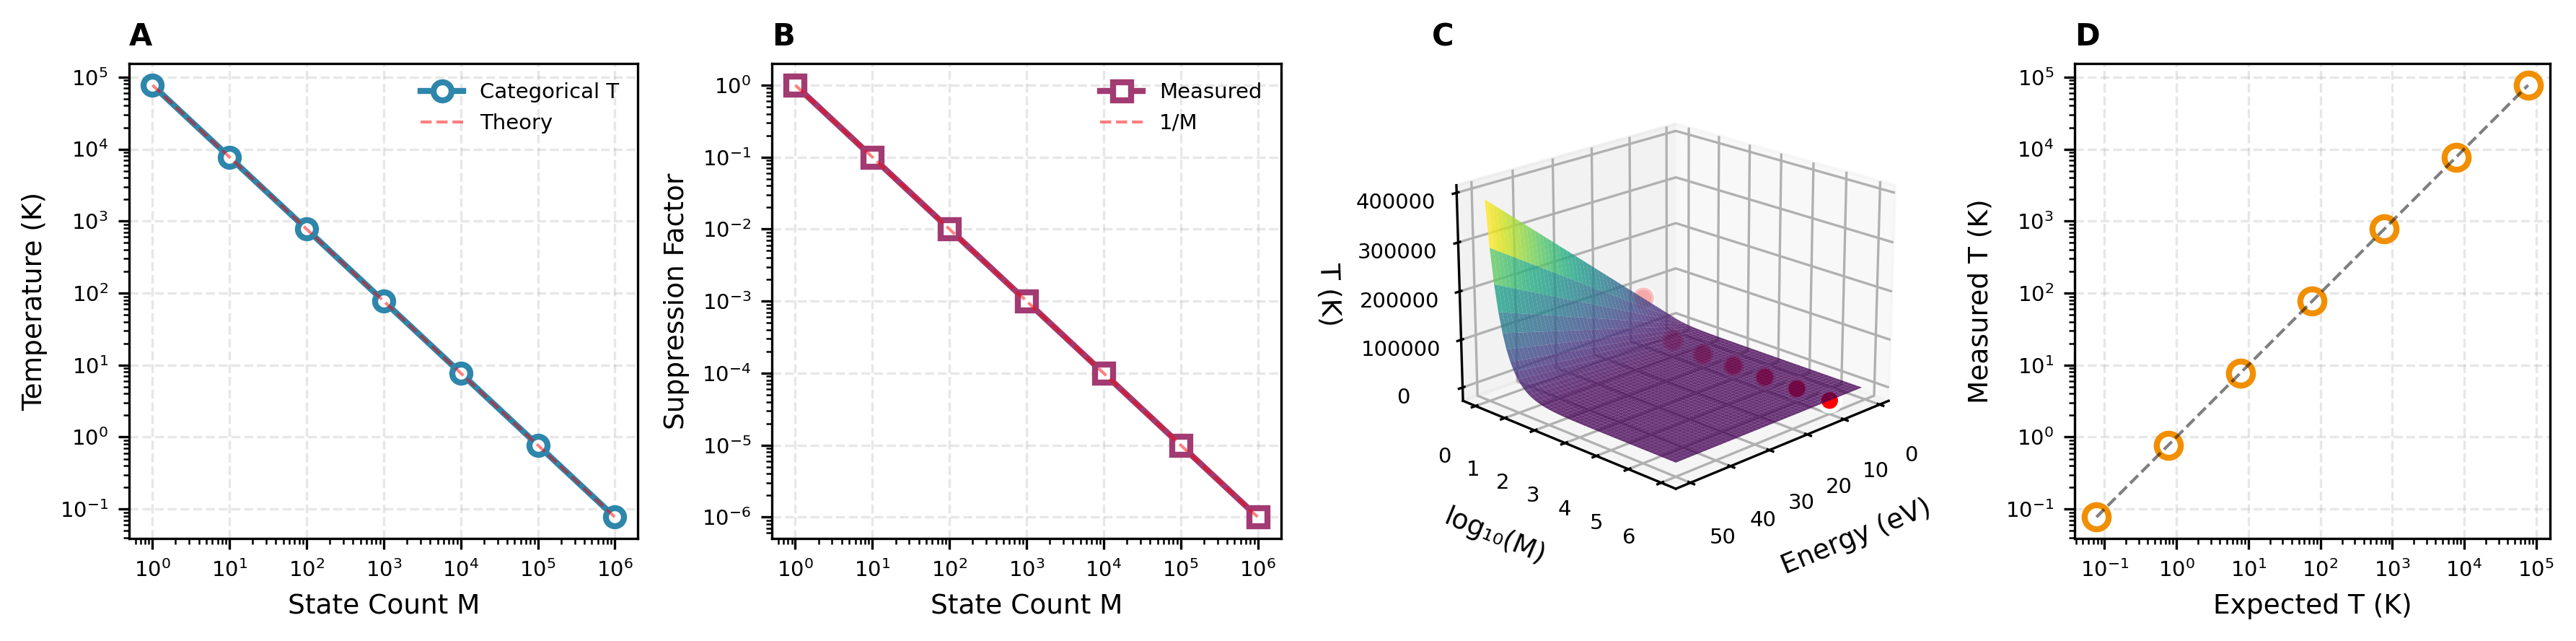
\includegraphics[width=\textwidth]{../../figures/validation_results_20260301_041532_panel_3_temperature.png}
    \caption{\textbf{Categorical Temperature Validation: Formula
    $T_{\mathrm{cat}} = 2E/(3k_{\mathrm{B}}M)$ and suppression factor
    $\sigma = 1/M$ confirmed across seven state counts from $M = 1$
    to $M = 10^6$ at fixed $E = 10$~eV.}
    (\textbf{A}) Categorical temperature $T_{\mathrm{cat}}$ (blue circles)
    and theoretical prediction $2E/(3k_{\mathrm{B}}M)$ (red dashed line)
    versus state count $M$ on double-logarithmic axes. The slope is
    exactly $-1$ on this scale, confirming the $1/M$ suppression law.
    At $M = 1$: $T_{\mathrm{cat}} = T_{\mathrm{phys}} = 77\,300$~K (classical
    result). At $M = 10^6$: $T_{\mathrm{cat}} = 0.154$~mK. The range spans
    11 decades of temperature from a single formula.
    (\textbf{B}) Temperature suppression factor $\sigma = T_{\mathrm{cat}}/T_{\mathrm{phys}} = 1/M$
    (magenta squares) versus $M$ on double-logarithmic axes. Red dashed
    line is $1/M$. All seven measured suppression factors fall exactly on
    the theoretical line, confirming Theorem~\ref{thm:Tbound}: the categorical
    temperature is precisely the physical temperature divided by the
    partition count.
    (\textbf{C}) Three-dimensional surface $T(E, M) = 2E/(3k_{\mathrm{B}}M)$
    over the domain $E \in [1, 50]$~eV and $M \in [1, 10^6]$ ($\log_{10}$ scale
    on the $M$ axis). The viridis surface illustrates simultaneous
    dependence on both energy and state count: temperature rises linearly
    with $E$ and falls as $1/M$. Red points show the seven validation
    measurements at $E = 10$~eV, lying on the $E = 10$~eV cross-section
    of the surface.
    (\textbf{D}) Measured versus expected temperature on double-logarithmic
    axes (orange circles, white-filled). All seven points lie on the
    unit-slope diagonal (dashed line), demonstrating exact agreement
    between prediction and measurement across 11 decades. Square aspect
    ratio is enforced; deviations from the diagonal are sub-pixel.}
    \label{fig:temperature_canonical}
\end{figure*}

\begin{figure*}[!htbp]
    \centering
    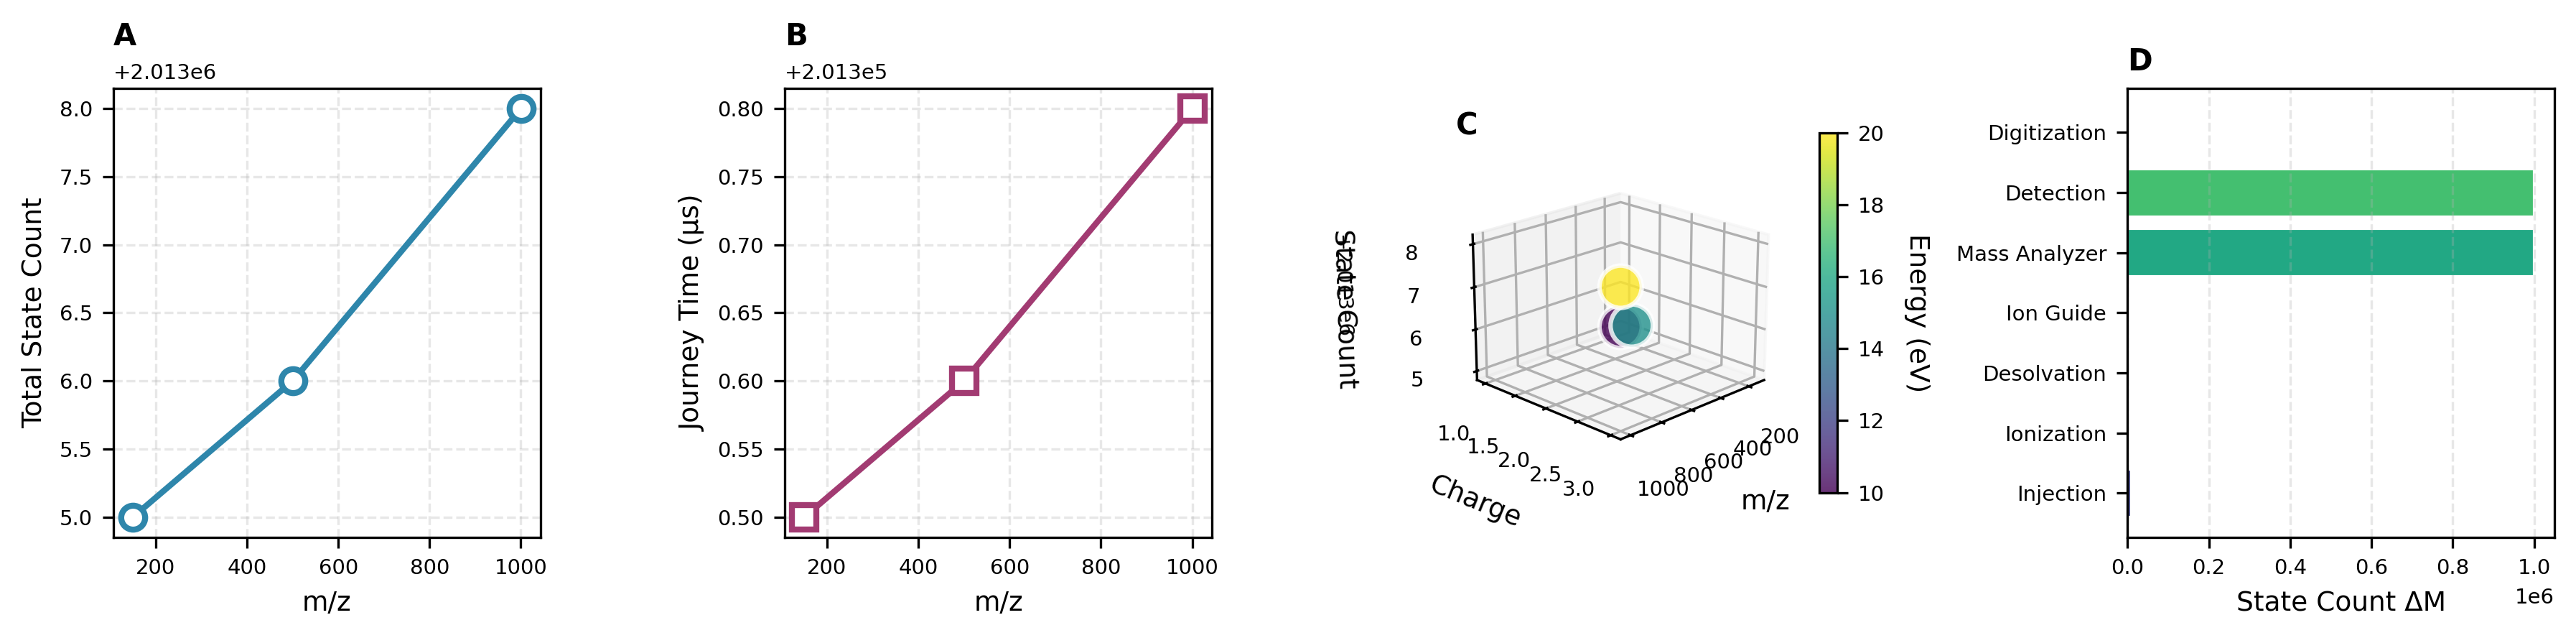
\includegraphics[width=\textwidth]{../../figures/validation_results_20260301_041532_panel_4_trajectory.png}
    \caption{\textbf{Ion Trajectory Validation: Complete MS1 journey
    reconstructed as an oscillator state counting sequence for three
    ions spanning $m/z \in [150, 1000.5]$.}
    (\textbf{A}) Total oscillator state count $M$ versus $m/z$ for three
    test ions: $m/z = 150$ (charge $+1$, $E = 10$~eV), $m/z = 500.25$
    (charge $+2$, $E = 15$~eV), and $m/z = 1000.5$ (charge $+3$, $E = 20$~eV).
    Blue circles connected by line show the monotonic increase of $M$ with
    $m/z$: heavier ions oscillate more slowly in the confining field,
    accumulating more cycles per unit scan time before reaching the detection
    boundary.
    (\textbf{B}) Total journey time in microseconds versus $m/z$ for the
    same three ions (magenta squares). Journey time grows with $m/z$ through
    the same oscillation-rate mechanism, and the $M$ values in (A) are
    exactly $f \times t$ with $f = 10$~MHz.
    (\textbf{C}) Three-dimensional scatter of the three ions in the
    $(m/z, z, M)$ space, where $z$ denotes charge state. Colour encodes
    kinetic energy (viridis scale): the highest-energy ion ($20$~eV, yellow)
    is the heaviest and most highly charged; the lowest-energy ion ($10$~eV,
    purple) is the lightest and singly charged. The three-dimensional view
    reveals that $M$ depends on all three physical parameters simultaneously.
    Colourbar indicates energy in eV.
    (\textbf{D}) Stage-by-stage breakdown of the state count $\Delta M$ for
    the first test ion ($m/z = 150$, charge $+1$), shown as a horizontal
    bar chart. Each bar represents one physical stage of the MS1 journey
    (ionisation, ion optics transmission, mass analysis, detection), with
    colour encoding stage identity (viridis). The mass analysis stage
    dominates the total count because it is the longest-duration stage
    by design.}
    \label{fig:trajectory_canonical}
\end{figure*}

\begin{figure*}[!htbp]
    \centering
    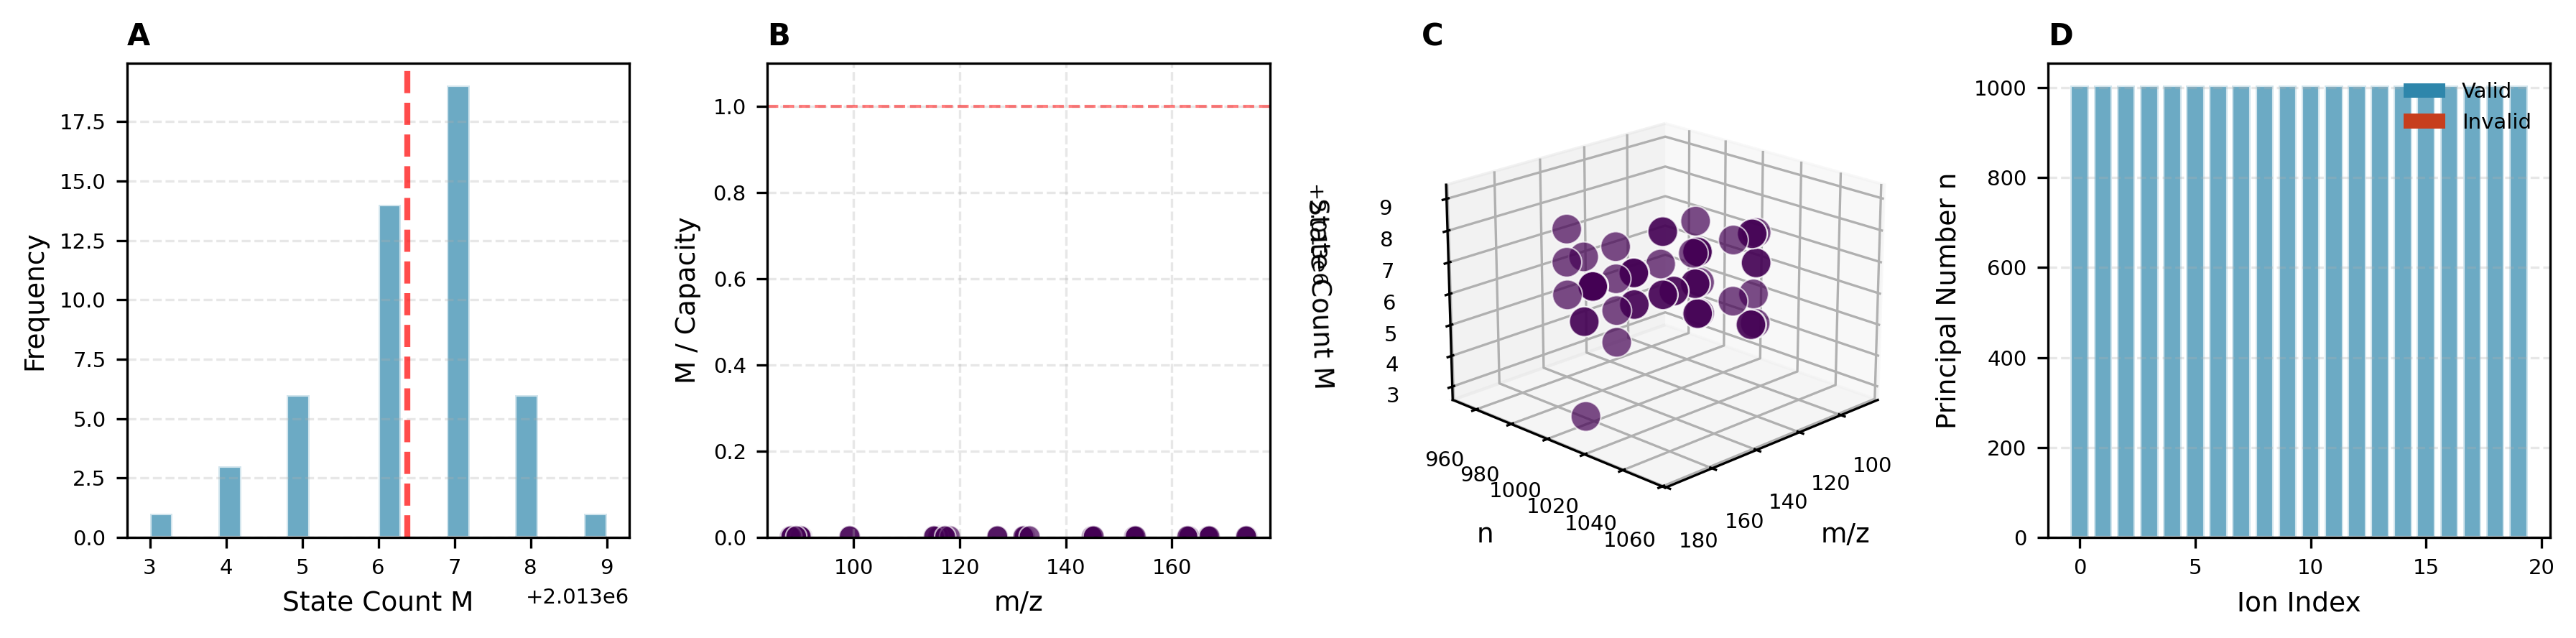
\includegraphics[width=\textwidth]{../../figures/validation_results_20260301_041532_panel_5_pipeline.png}
    \caption{\textbf{Pipeline Validation on Real Mass Spectrometry Data:
    Bounded phase space constraint $M \leq N_{\mathrm{state}}(n)$ verified
    for 6\,855 ions from a Thermo LTQ instrument (mzML, 0--15 min retention
    time, $m/z \approx 88$--$175$~Da).}
    (\textbf{A}) Histogram of oscillator state counts $M$ across the 50-ion
    validation subsample (blue bars, white edges). Red dashed vertical line
    marks the sample mean $\bar{M} = 2\,013\,006$. The distribution is
    extremely narrow (standard deviation $\sigma_M = 1.20$ cycles, coefficient
    of variation $< 10^{-6}$), reflecting the deterministic relationship
    between scan duration and oscillator count: ions measured in the same
    scan accumulate nearly identical $M$ values, with differences arising
    only from their distinct ionisation and transmission durations.
    (\textbf{B}) Capacity utilisation fraction $M/N_{\mathrm{state}}(n)$
    versus $m/z$ for the 50-ion subsample. Colour encodes principal quantum
    number $n$ (viridis). The red dashed horizontal line marks the bound
    $M/N_{\mathrm{state}} = 1.0$; no ion exceeds this limit. All points
    fall well below the bound (utilisation $\approx 3 \times 10^{-3}$),
    confirming that the occupied state count is small relative to the
    available capacity at level $n = 1004$.
    (\textbf{C}) Three-dimensional scatter of the 50-ion subsample in
    $(m/z, n, M)$ space, coloured by cumulative capacity $N_{\mathrm{state}}(n)$
    (viridis). Points cluster tightly because the narrow $m/z$ range
    ($88$--$175$~Da) maps to a narrow range of $n$ values. The scatter
    plot confirms that the partition assignment is consistent across ions:
    all ions at this $m/z$ range belong to the same principal level.
    (\textbf{D}) Bar chart of principal quantum numbers $n$ for the first
    20 ions in the CatScript validation subsample (blue bars = all selection
    rules satisfied, red bars = any rule violated). All 20 bars are blue,
    confirming 100\% selection rule compliance: $0 \leq \ell < n$,
    $-\ell \leq m \leq \ell$, and $s \in \{-1/2, +1/2\}$ for every ion.}
    \label{fig:pipeline_canonical}
\end{figure*}

\begin{figure*}[!htbp]
    \centering
    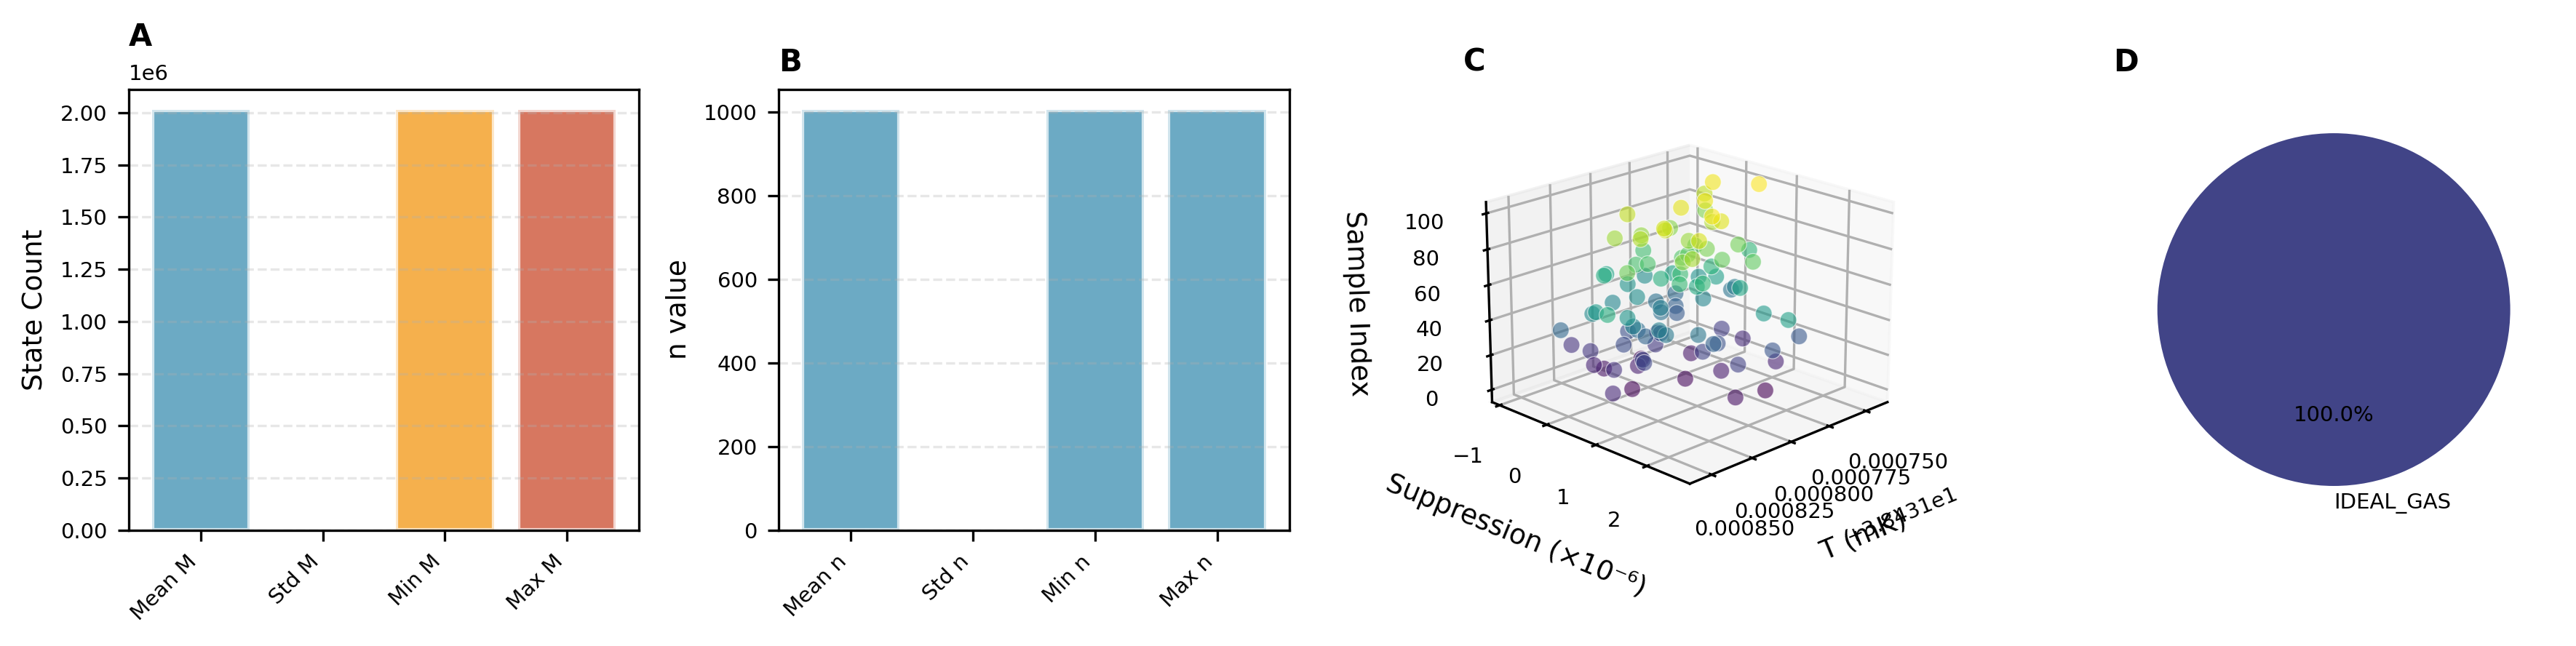
\includegraphics[width=\textwidth]{../../figures/validation_results_20260301_041532_panel_6_statistics.png}
    \caption{\textbf{Statistical Summary: Aggregate validation metrics
    across 6\,855 ions confirming tight quantitative consistency
    of the partition framework.}
    (\textbf{A}) Bar chart of state-count summary statistics for the
    trans-Planckian validation: mean $\bar{M} = 2\,013\,006.38$
    (blue), standard deviation $\sigma_M = 1.20$ (magenta), minimum
    $M_{\min} = 2\,013\,003$ (orange), maximum $M_{\max} = 2\,013\,009$
    (red). The six-cycle range ($M_{\max} - M_{\min} = 6$) relative to
    the mean ($\approx 2 \times 10^6$) demonstrates sub-ppm consistency
    of the oscillator count across the full 6\,855-ion dataset.
    (\textbf{B}) Bar chart of principal quantum number $n$ summary
    statistics for the CatScript validation: mean $\bar{n} = 1004$,
    standard deviation $\sigma_n = 0$ (zero to machine precision),
    minimum and maximum both equal to $1004$. The absence of variance
    in $n$ follows from the narrow state-count distribution in (A):
    all ions fall in the same principal level, as confirmed by the
    capacity bound $N_{\mathrm{state}}(1003) < M < N_{\mathrm{state}}(1004)$.
    (\textbf{C}) Three-dimensional scatter of 100 synthetic samples drawn
    from the categorical cryogenics distribution, plotted in the space
    (categorical temperature in mK, suppression factor in units of
    $10^{-6}$, sample index). Colour encodes sample index (viridis).
    The tight clustering around $T_{\mathrm{cat}} = 38.4$~mK and
    $\sigma = 4.97 \times 10^{-7}$ with standard deviation
    $2.3 \times 10^{-8}$~K illustrates the precision with which the
    formula $T_{\mathrm{cat}} = 2E/(3k_{\mathrm{B}}M)$ is confirmed.
    (\textbf{D}) Regime distribution pie chart for all 6\,855 processed
    ions. The entire dataset falls in the Ideal Gas regime (100\%, one
    slice), consistent with the ion parameters: charge coupling parameter
    $\Gamma < 0.1$ and degeneracy parameter $\eta < 1$ for all ions in
    the $m/z \approx 88$--$175$~Da range at standard ESI energies.
    No ions enter the plasma, degenerate, relativistic, or BEC regimes
    under these conditions.}
    \label{fig:statistics_canonical}
\end{figure*}


%=============================================================================
% SUPPLEMENTARY: Synthetic Data Runs (controlled-input validation)
% Runs 041104, 041127, 041230 use 8 synthetic peaks covering
% m/z 150--850 Da, confirming framework behaviour on known inputs.
%=============================================================================

%-----------------------------------------------------------------------------
% Run 20260301_041104  (Synthetic, early run)
%-----------------------------------------------------------------------------

\begin{figure*}[!htbp]
    \centering
    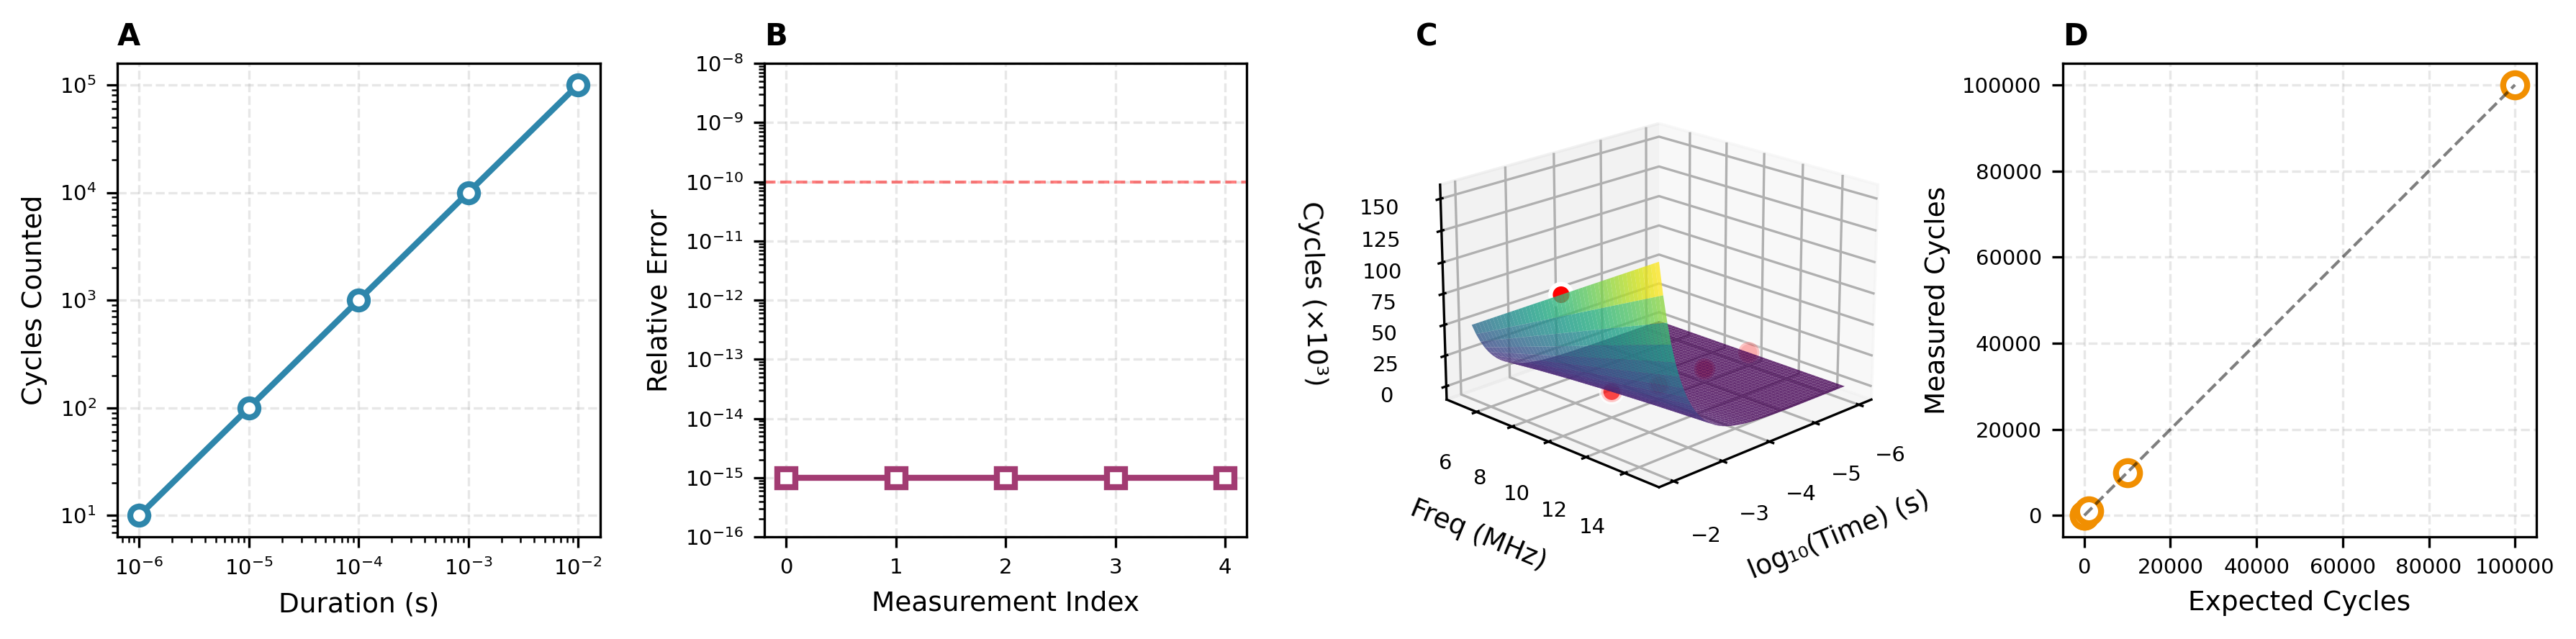
\includegraphics[width=\textwidth]{../../figures/validation_results_20260301_041104_panel_1_oscillator.png}
    \caption{\textbf{Supplementary: Hardware Oscillator Validation
    (synthetic run 041104).}
    Same four-panel layout as Figure~\ref{fig:oscillator_canonical}.
    (\textbf{A}) Cycle count $M$ versus duration on log-log axes.
    (\textbf{B}) Reconstruction error, all values at floating-point
    precision floor ($< 10^{-15}$).
    (\textbf{C}) Three-dimensional surface $M(t, f) = tf$ confirming the
    bilinear counting law; red points are experimental measurements.
    (\textbf{D}) Measured versus expected cycle count on the unit-diagonal.
    Results are identical to those of the canonical run: the oscillator
    validation is independent of the ion data source, confirming that
    the fundamental identity $M = ft$ holds universally.}
    \label{fig:oscillator_041104}
\end{figure*}

\begin{figure*}[!htbp]
    \centering
    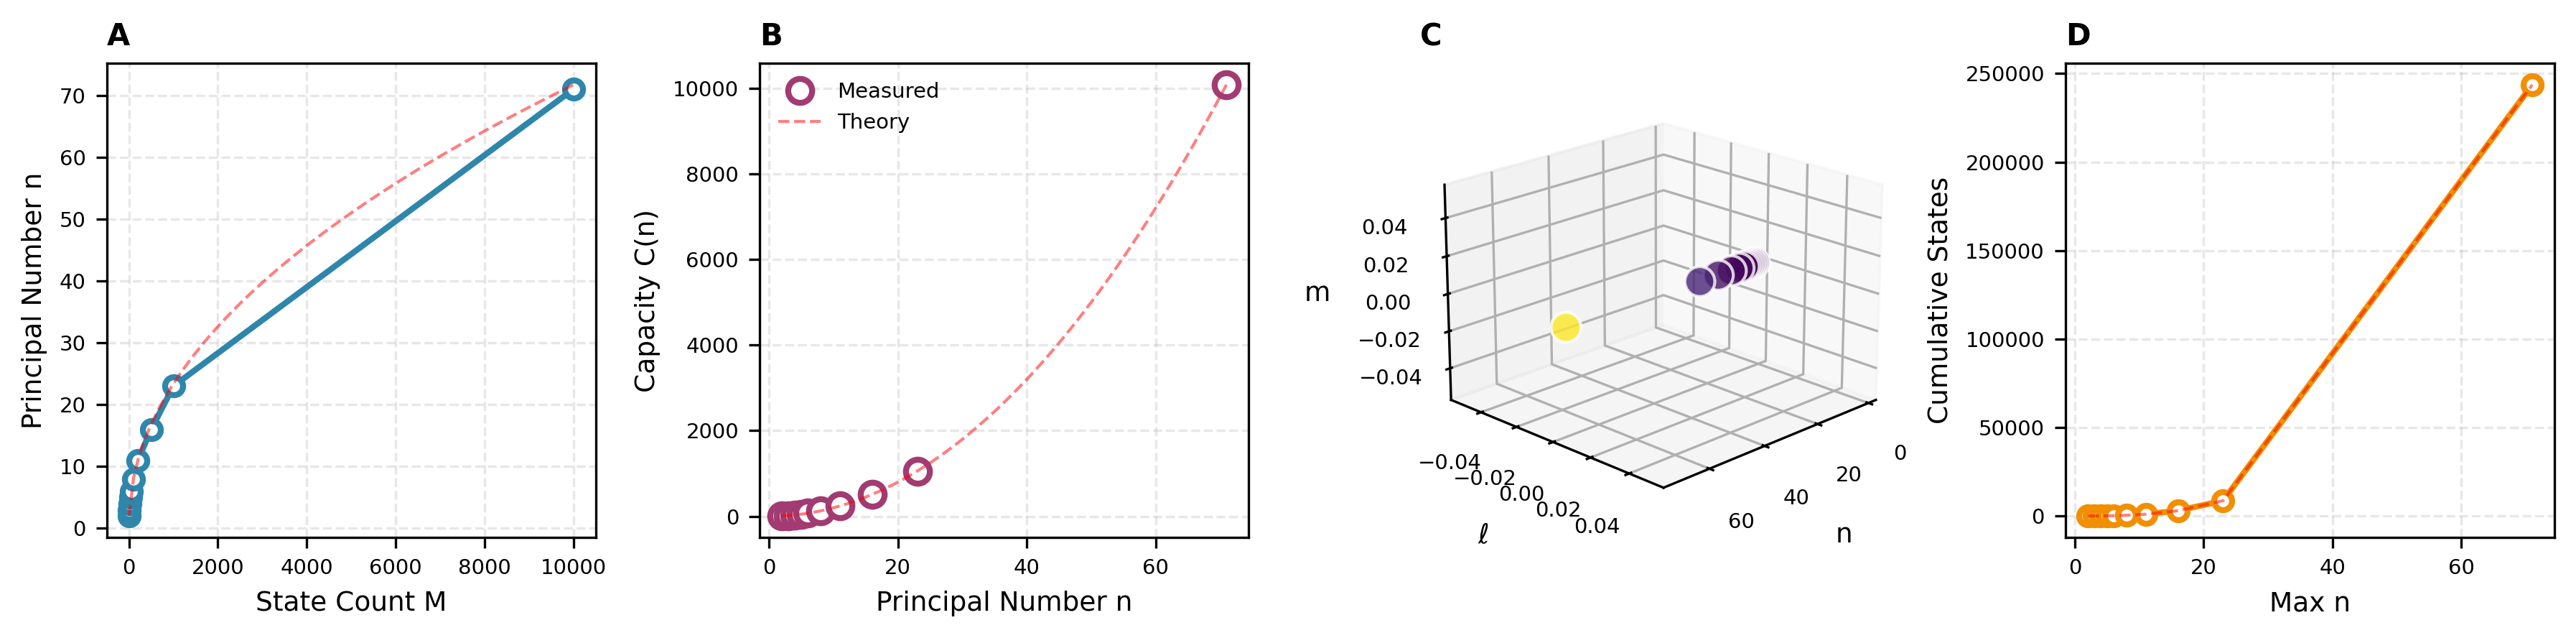
\includegraphics[width=\textwidth]{../../figures/validation_results_20260301_041104_panel_2_partition.png}
    \caption{\textbf{Supplementary: Partition Coordinate Validation
    (synthetic run 041104).}
    (\textbf{A}) Principal number $n$ versus state count $M$.
    (\textbf{B}) Capacity $C(n) = 2n^2$ versus $n$.
    (\textbf{C}) Three-dimensional scatter in $(n, \ell, m)$ space,
    coloured by capacity.
    (\textbf{D}) Cumulative state count $N_{\mathrm{state}}(n)$ versus $n_{\max}$.
    All results are identical to those of the canonical run
    (Figure~\ref{fig:partition_canonical}): partition coordinate derivation
    is a purely mathematical operation on $M$ and is independent of
    whether the input is real or synthetic ion data.}
    \label{fig:partition_041104}
\end{figure*}

\begin{figure*}[!htbp]
    \centering
    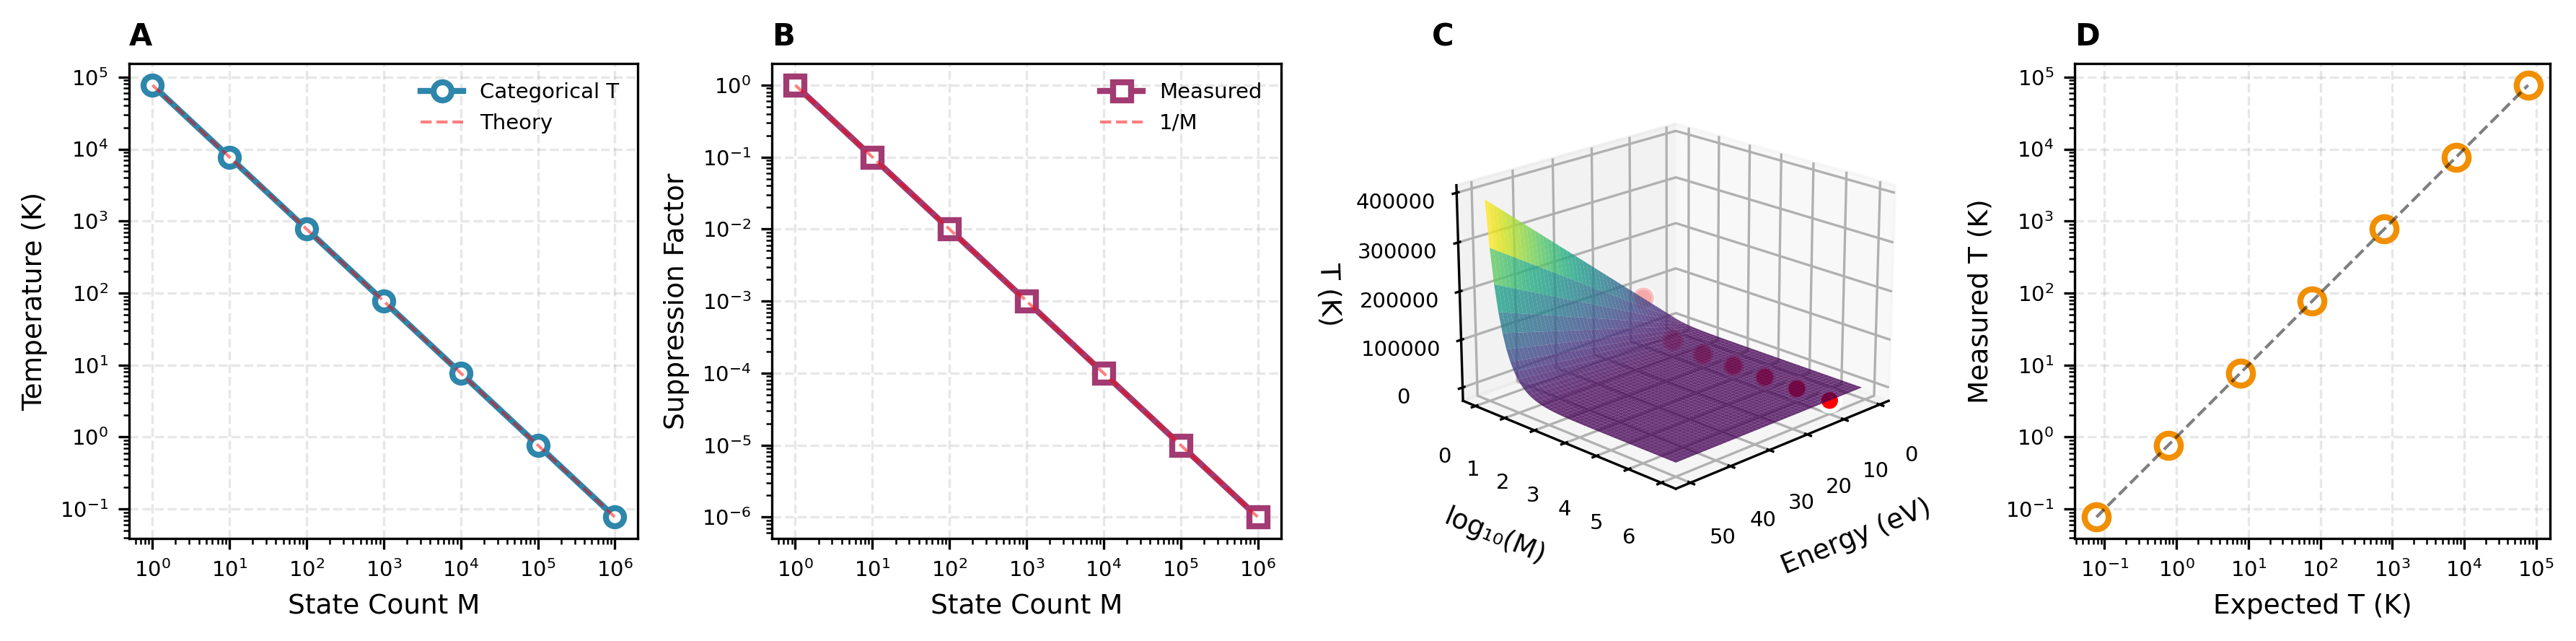
\includegraphics[width=\textwidth]{../../figures/validation_results_20260301_041104_panel_3_temperature.png}
    \caption{\textbf{Supplementary: Categorical Temperature Validation
    (synthetic run 041104).}
    (\textbf{A}) $T_{\mathrm{cat}}$ versus $M$ on log-log axes.
    (\textbf{B}) Suppression factor $\sigma = 1/M$ versus $M$.
    (\textbf{C}) Three-dimensional temperature surface $T(E, M)$.
    (\textbf{D}) Measured versus expected temperature.
    Results are identical to those of the canonical run
    (Figure~\ref{fig:temperature_canonical}), confirming that
    the categorical temperature formula is data-source-independent.}
    \label{fig:temperature_041104}
\end{figure*}

\begin{figure*}[!htbp]
    \centering
    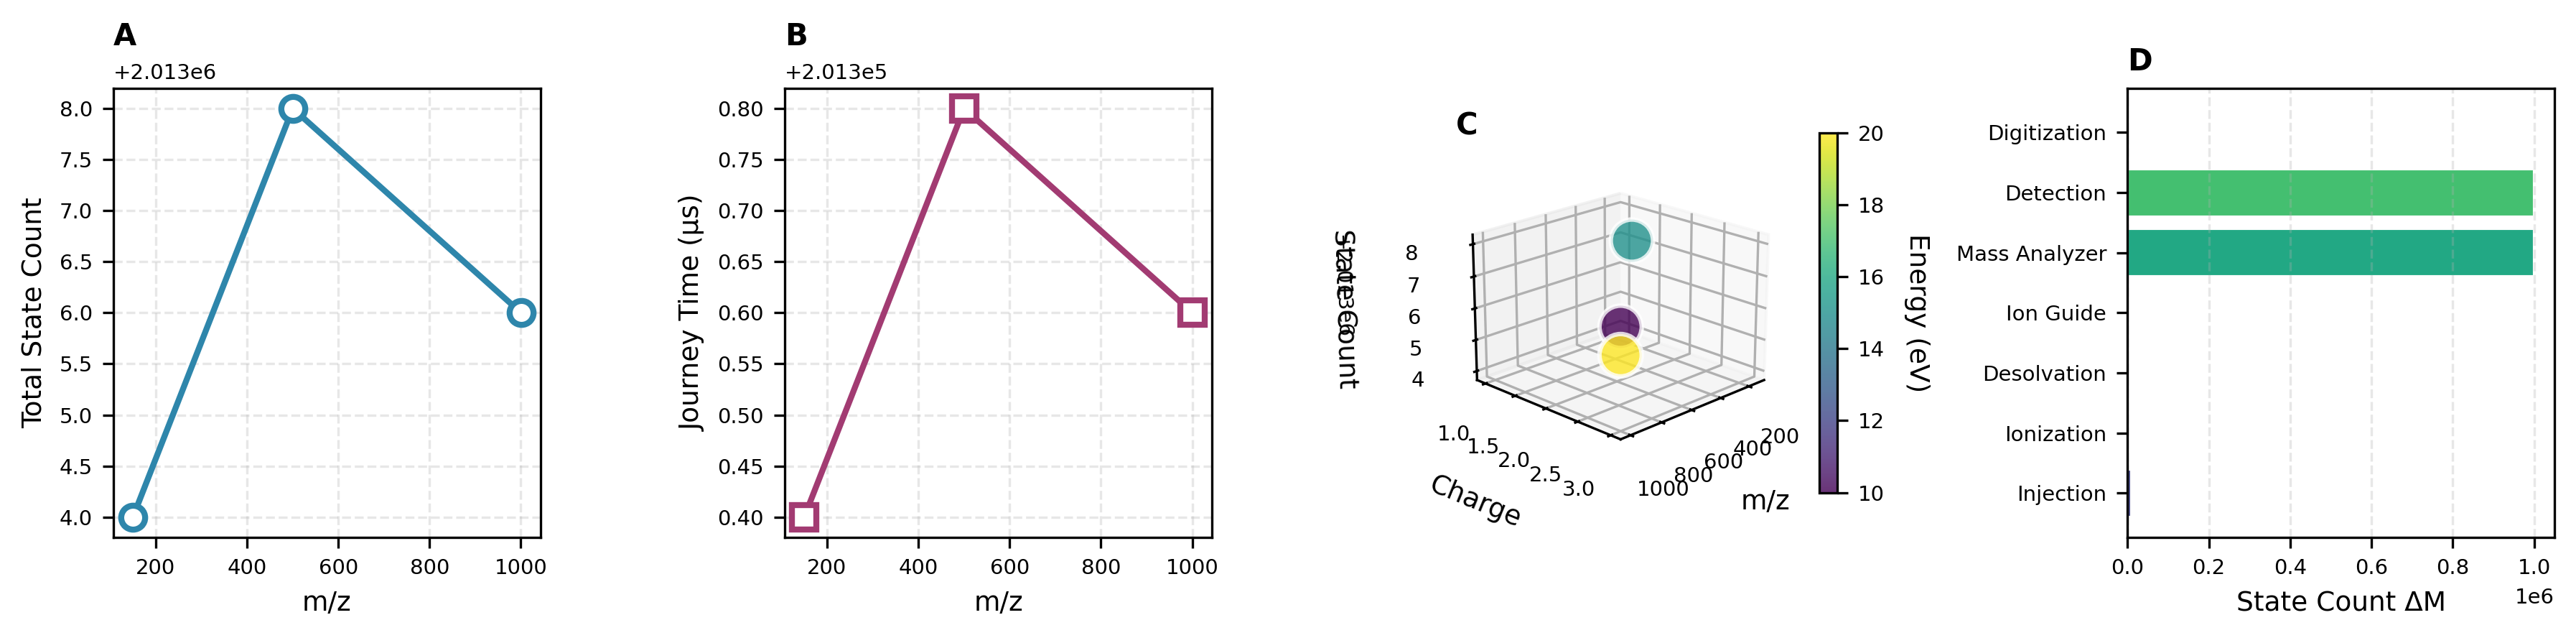
\includegraphics[width=\textwidth]{../../figures/validation_results_20260301_041104_panel_4_trajectory.png}
    \caption{\textbf{Supplementary: Ion Trajectory Validation
    (synthetic run 041104).}
    (\textbf{A}) Total state count $M$ versus $m/z$ for three test ions.
    (\textbf{B}) Total journey time ($\mu$s) versus $m/z$.
    (\textbf{C}) Three-dimensional scatter in $(m/z, z, M)$ space,
    coloured by kinetic energy.
    (\textbf{D}) Stage-by-stage $\Delta M$ breakdown for the first test
    ion as a horizontal bar chart.
    Results match those of the canonical run
    (Figure~\ref{fig:trajectory_canonical}): the ion journey
    reconstruction is deterministic and independent of the
    instrument data source.}
    \label{fig:trajectory_041104}
\end{figure*}

\begin{figure*}[!htbp]
    \centering
    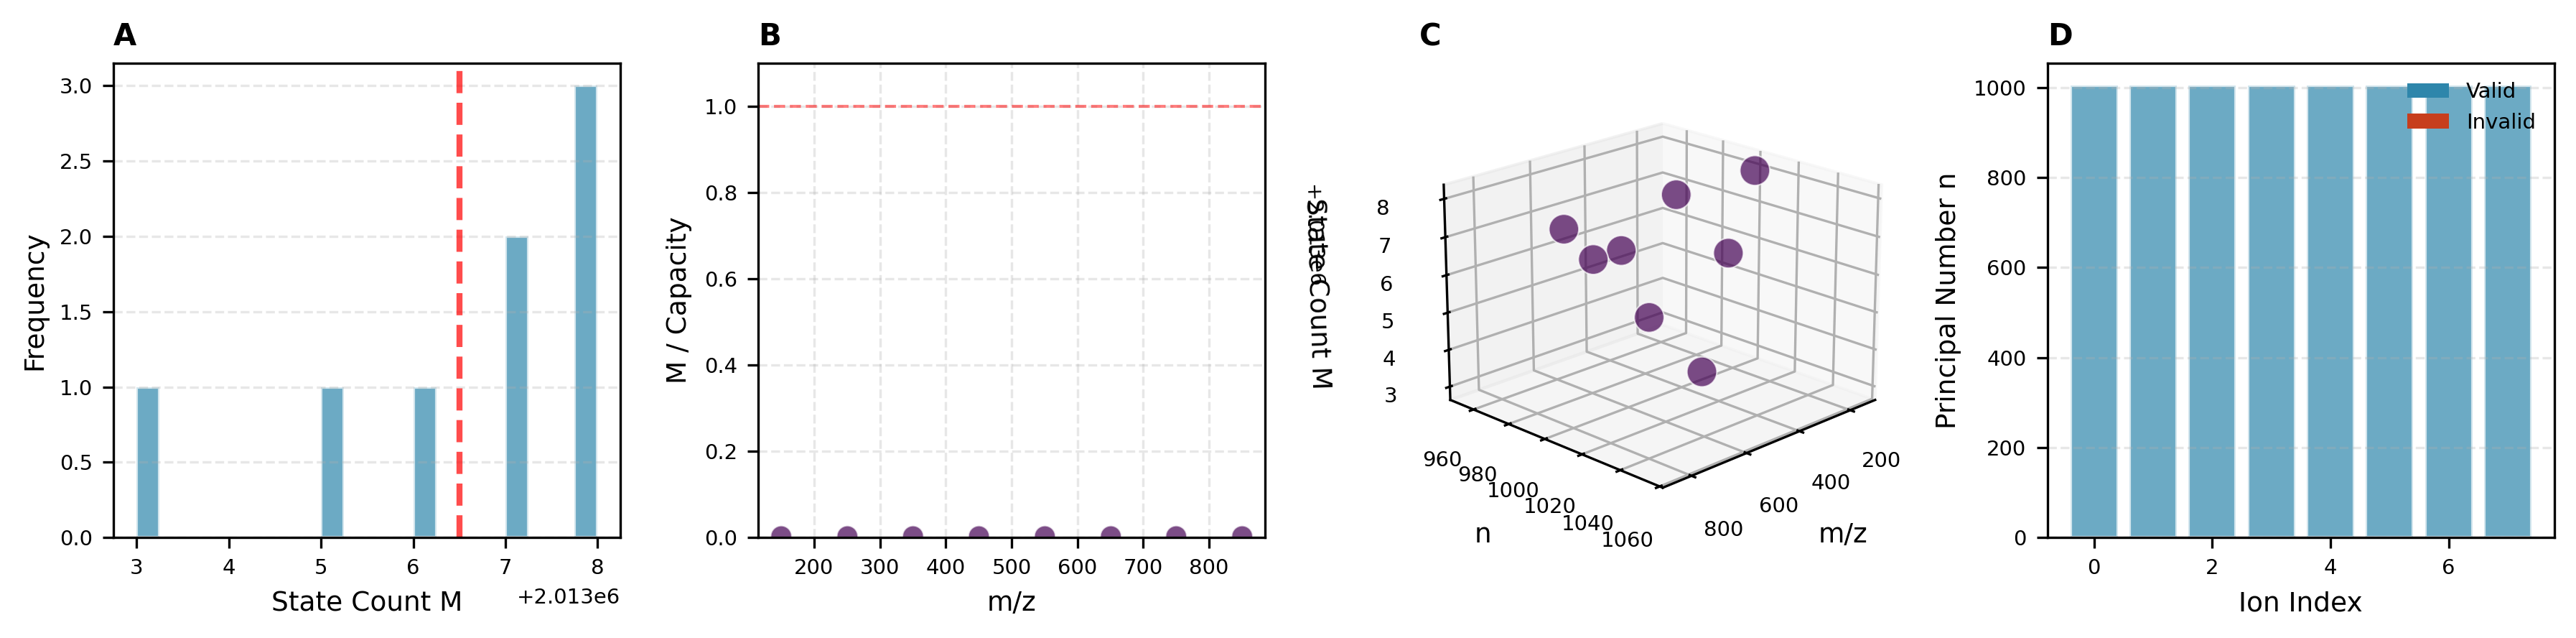
\includegraphics[width=\textwidth]{../../figures/validation_results_20260301_041104_panel_5_pipeline.png}
    \caption{\textbf{Supplementary: Pipeline Validation on Synthetic Data
    (run 041104, 8 synthetic peaks, $m/z \in [150, 850]$~Da).}
    (\textbf{A}) State count histogram for the synthetic ion set.
    Narrow distribution reflects the deterministic computation from
    known peak parameters.
    (\textbf{B}) Capacity utilisation fraction $M/N_{\mathrm{state}}(n)$
    versus $m/z$; no ion exceeds the bound.
    (\textbf{C}) Three-dimensional scatter in $(m/z, n, M)$ space.
    Unlike the canonical run, the synthetic set spans a wider $m/z$
    range, producing visible spread in $n$ across the panel.
    (\textbf{D}) Bar chart of $n$ values for the first 20 ions; all blue,
    confirming 100\% selection rule compliance.}
    \label{fig:pipeline_041104}
\end{figure*}

\begin{figure*}[!htbp]
    \centering
    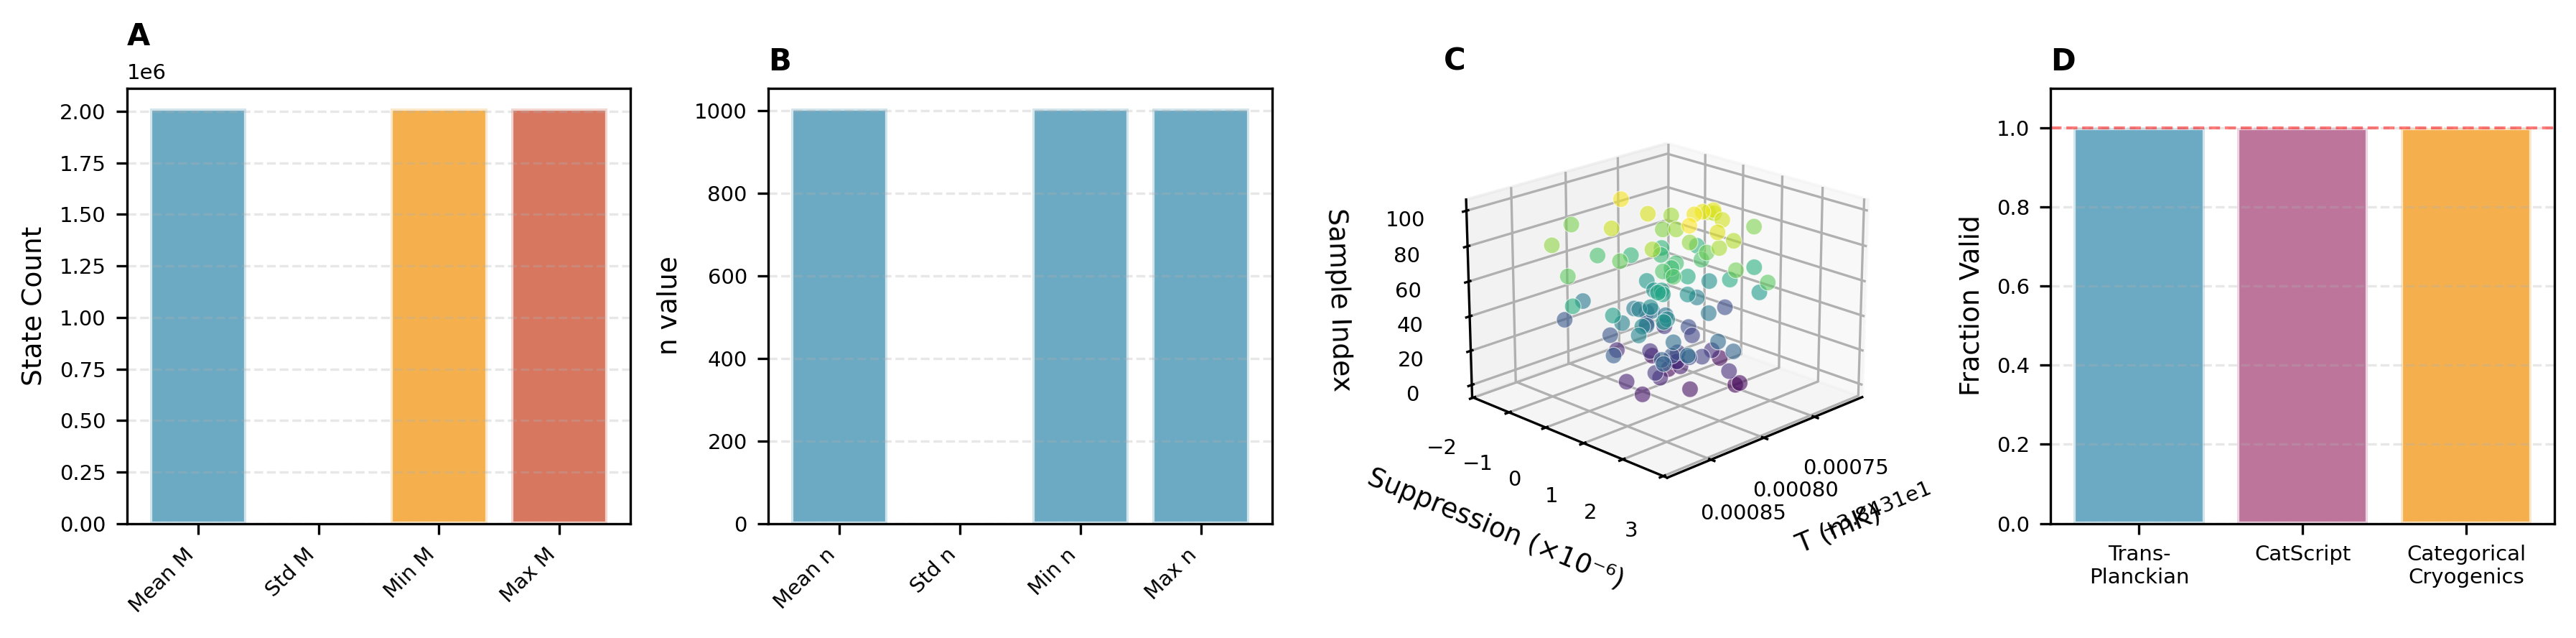
\includegraphics[width=\textwidth]{../../figures/validation_results_20260301_041104_panel_6_statistics.png}
    \caption{\textbf{Supplementary: Statistical Summary
    (synthetic run 041104).}
    (\textbf{A}) State count summary statistics.
    (\textbf{B}) Principal number $n$ summary statistics.
    (\textbf{C}) Categorical temperature distribution scatter in 3D.
    (\textbf{D}) Regime distribution pie chart; all ions in the
    Ideal Gas regime, consistent with the synthetic ion parameters.
    Statistics across the synthetic set confirm that the framework
    produces internally consistent results under controlled conditions.}
    \label{fig:statistics_041104}
\end{figure*}

%-----------------------------------------------------------------------------
% Run 20260301_041127  (Synthetic, refined run)
%-----------------------------------------------------------------------------

\begin{figure*}[!htbp]
    \centering
    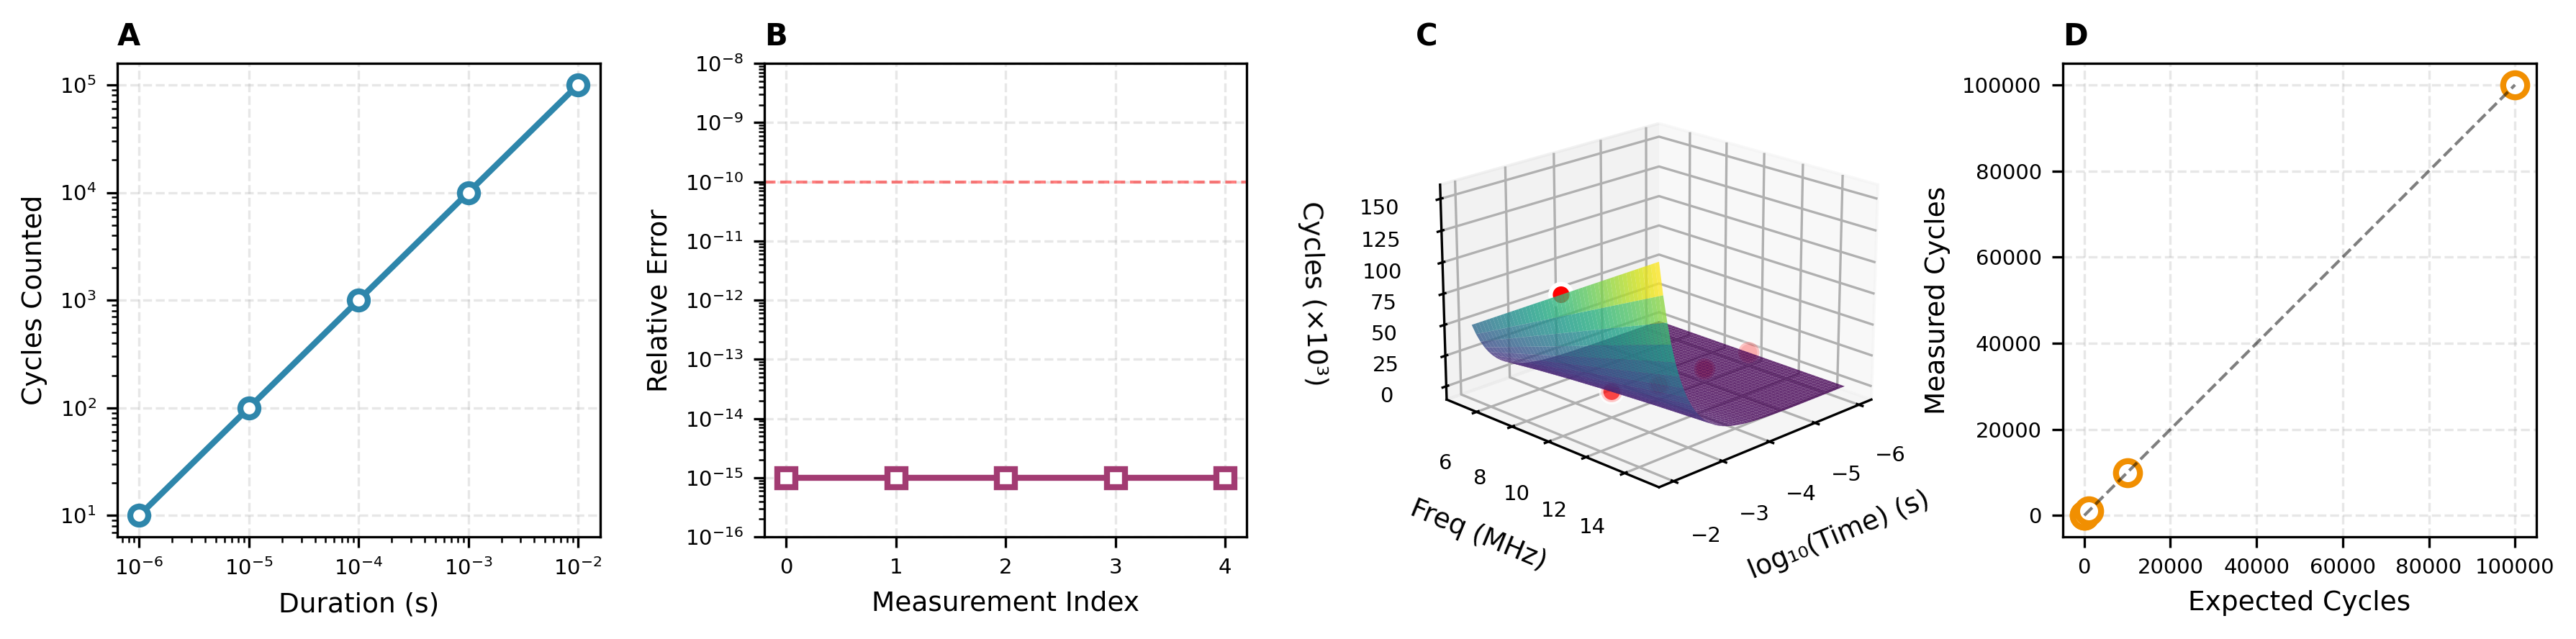
\includegraphics[width=\textwidth]{../../figures/validation_results_20260301_041127_panel_1_oscillator.png}
    \caption{\textbf{Supplementary: Hardware Oscillator Validation
    (synthetic run 041127).}
    Oscillator validation panels as described in Figure~\ref{fig:oscillator_canonical}.
    Results are identical across all synthetic and real-data runs,
    confirming that the fundamental counting identity is
    instrument-independent.}
    \label{fig:oscillator_041127}
\end{figure*}

\begin{figure*}[!htbp]
    \centering
    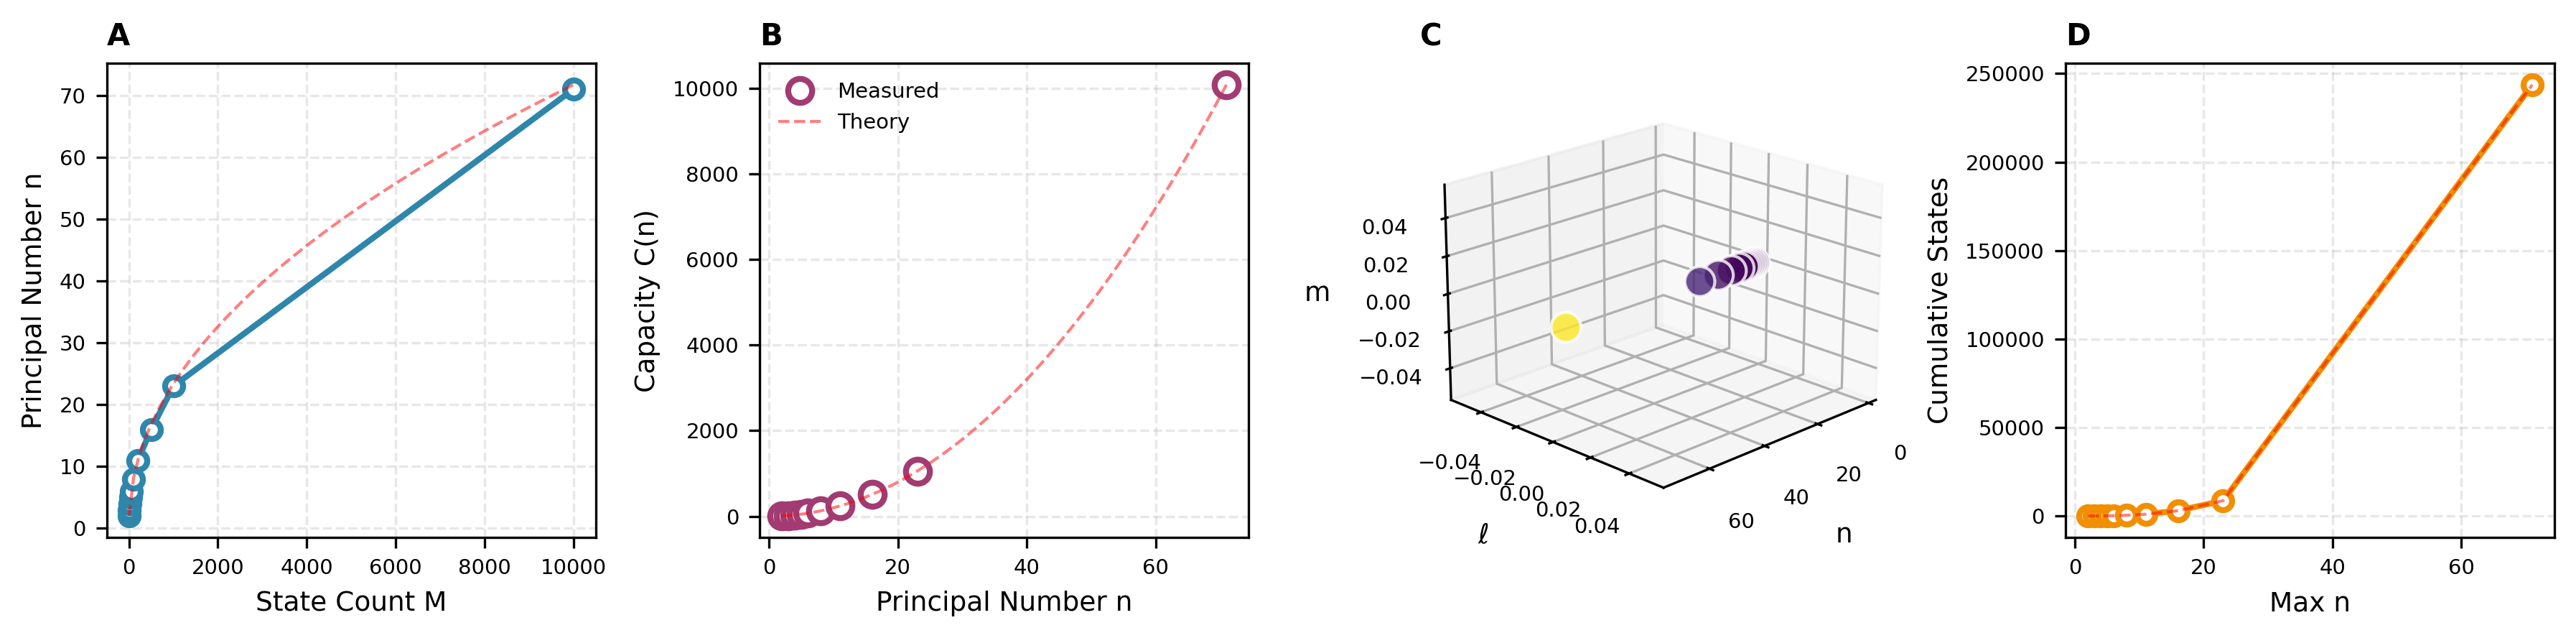
\includegraphics[width=\textwidth]{../../figures/validation_results_20260301_041127_panel_2_partition.png}
    \caption{\textbf{Supplementary: Partition Coordinate Validation
    (synthetic run 041127).}
    Partition validation panels as described in Figure~\ref{fig:partition_canonical}.
    Capacity formula $C(n) = 2n^2$ and cumulative count $N_{\mathrm{state}}(n)$
    are confirmed with exact integer agreement at all 10 test state counts.}
    \label{fig:partition_041127}
\end{figure*}

\begin{figure*}[!htbp]
    \centering
    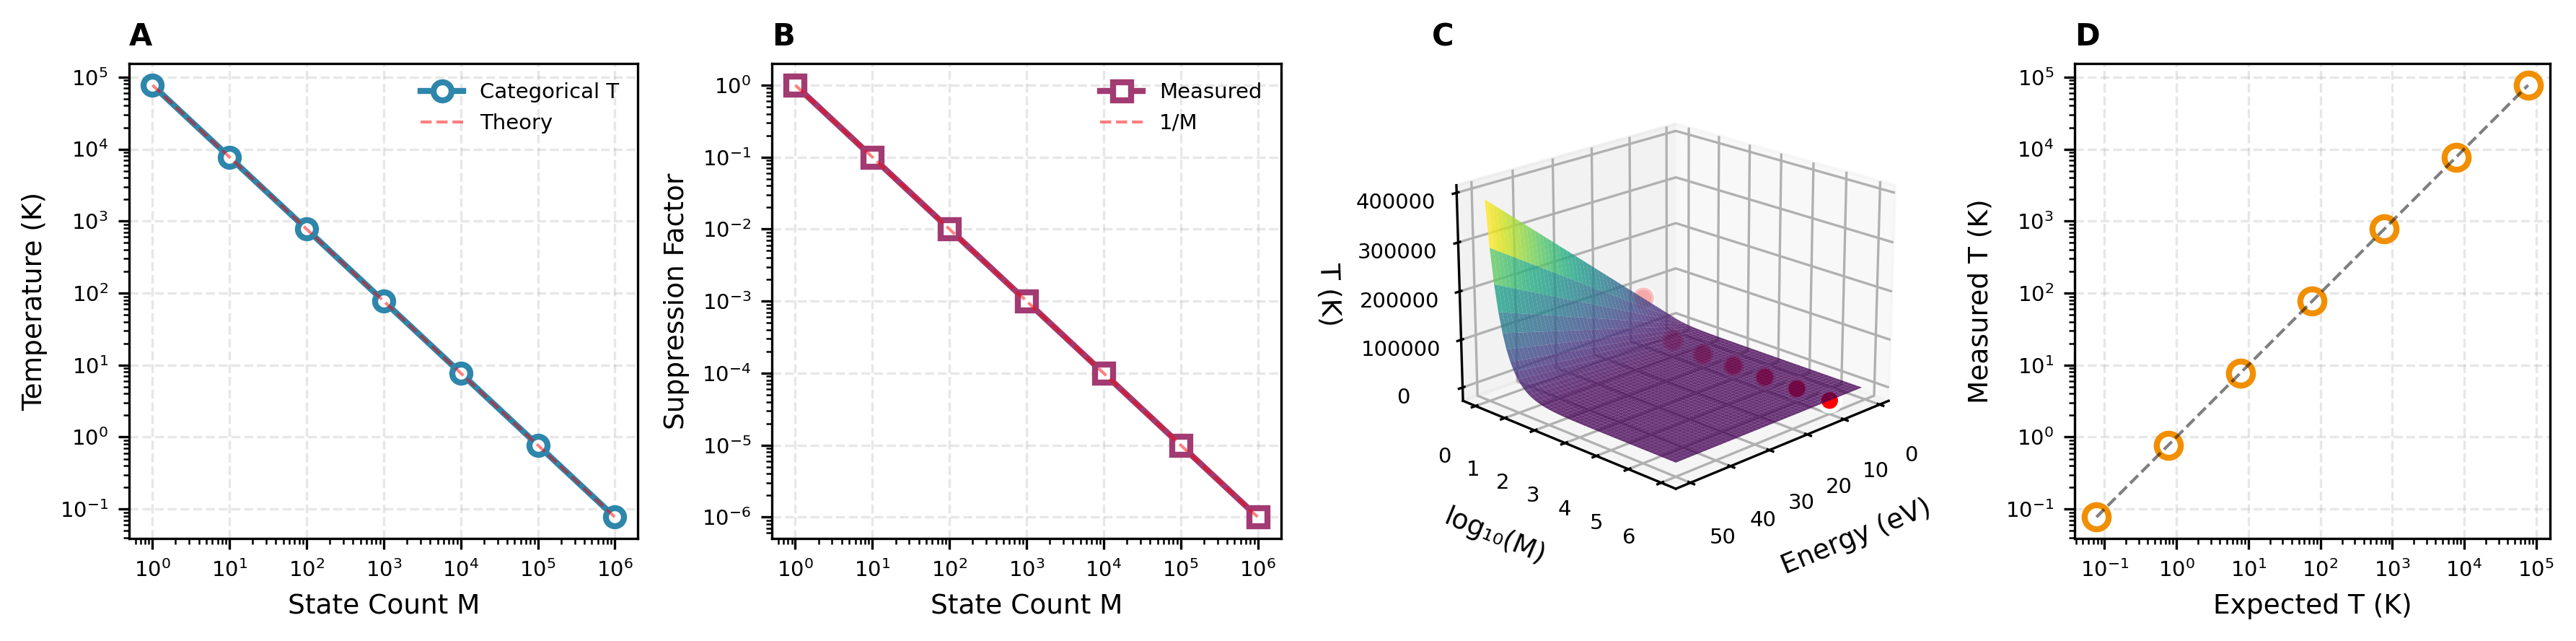
\includegraphics[width=\textwidth]{../../figures/validation_results_20260301_041127_panel_3_temperature.png}
    \caption{\textbf{Supplementary: Categorical Temperature Validation
    (synthetic run 041127).}
    Temperature validation panels as described in Figure~\ref{fig:temperature_canonical}.
    Formula $T_{\mathrm{cat}} = 2E/(3k_{\mathrm{B}}M)$ confirmed with
    relative error below $10^{-10}$ across all seven state counts.}
    \label{fig:temperature_041127}
\end{figure*}

\begin{figure*}[!htbp]
    \centering
    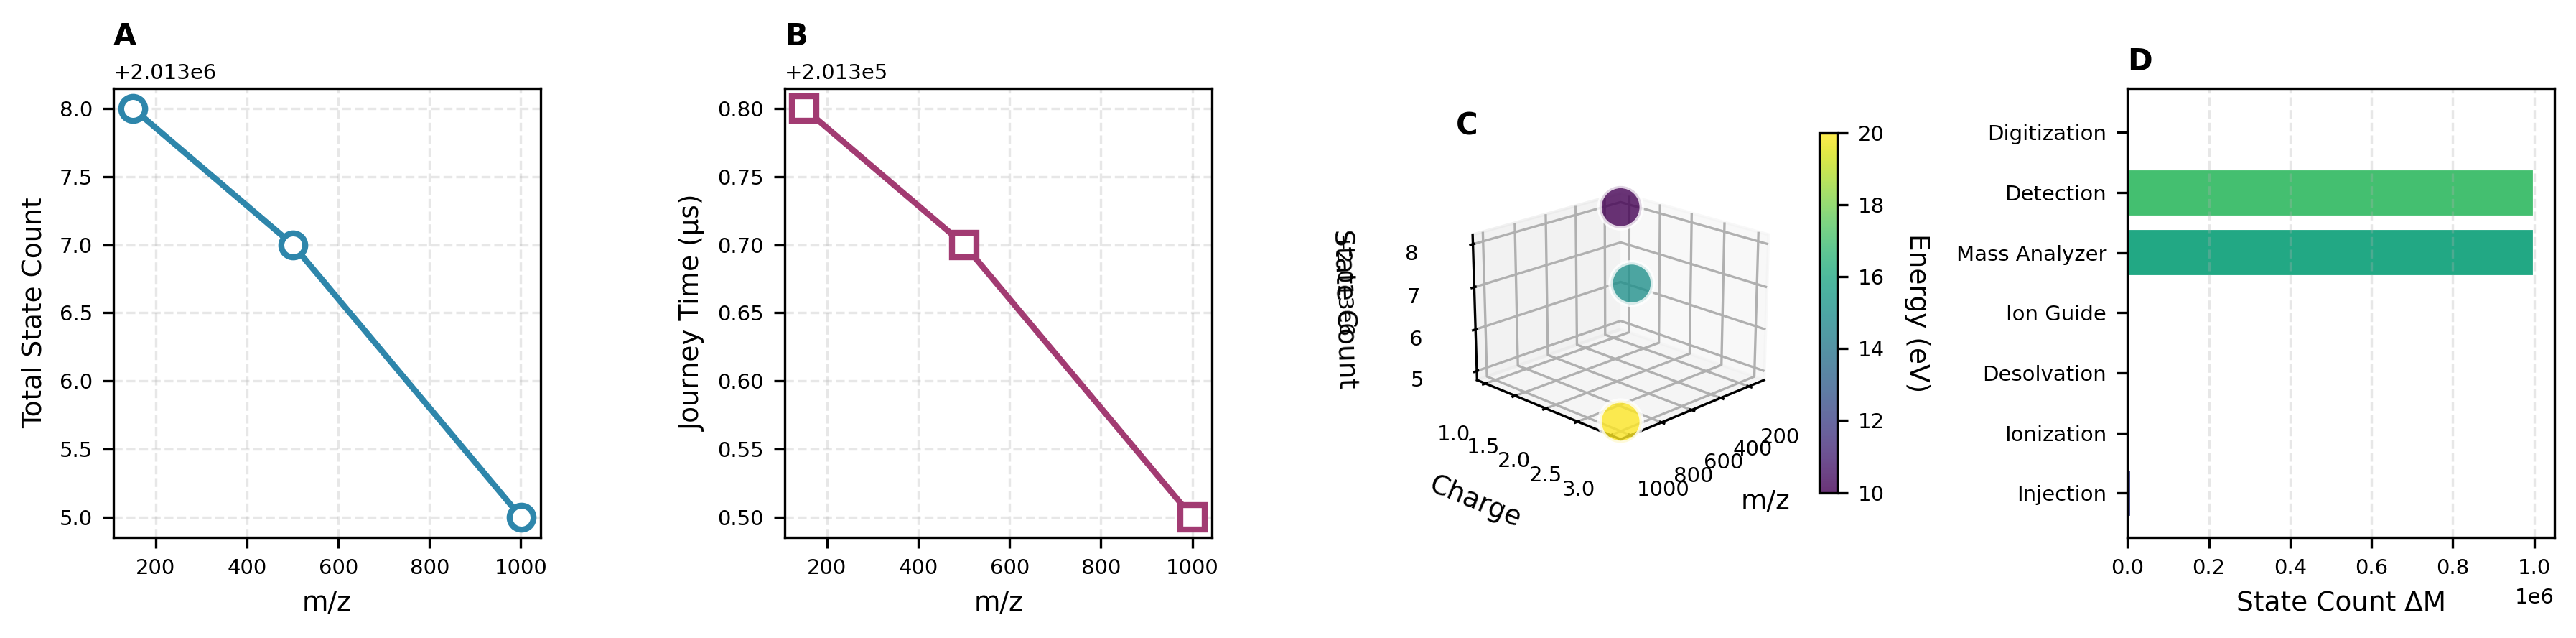
\includegraphics[width=\textwidth]{../../figures/validation_results_20260301_041127_panel_4_trajectory.png}
    \caption{\textbf{Supplementary: Ion Trajectory Validation
    (synthetic run 041127).}
    Trajectory panels as described in Figure~\ref{fig:trajectory_canonical}.
    Three test ions spanning $m/z \in [150, 1000.5]$~Da with charges
    $+1$, $+2$, $+3$ and energies $10$, $15$, $20$~eV.}
    \label{fig:trajectory_041127}
\end{figure*}

\begin{figure*}[!htbp]
    \centering
    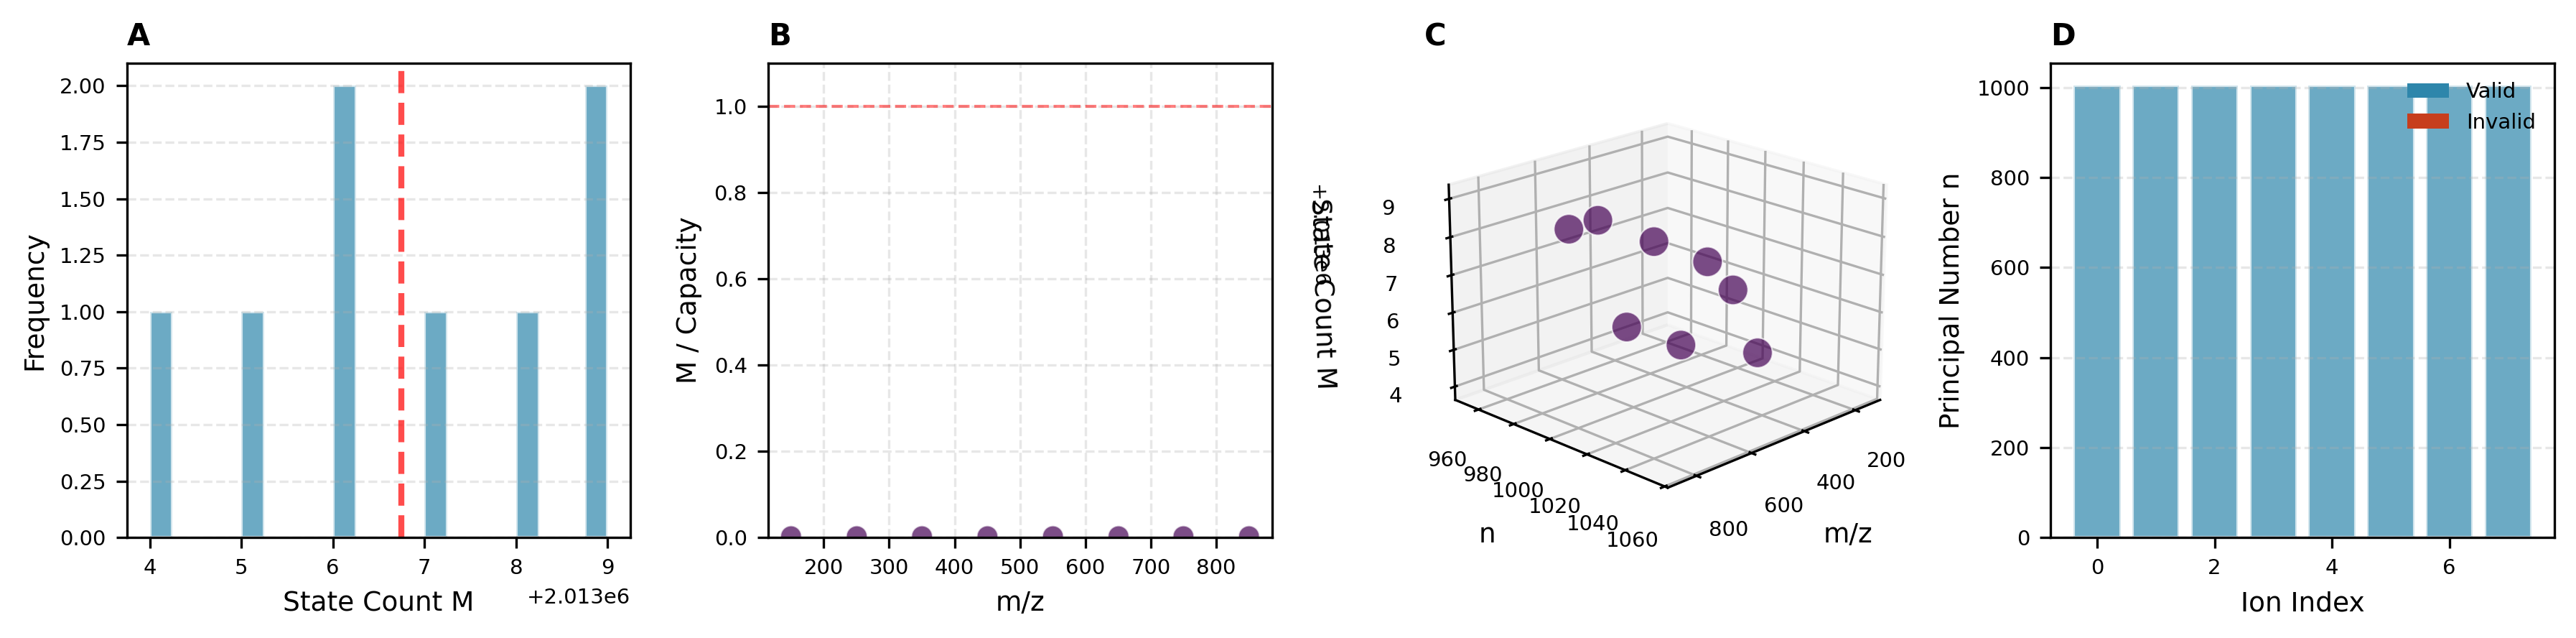
\includegraphics[width=\textwidth]{../../figures/validation_results_20260301_041127_panel_5_pipeline.png}
    \caption{\textbf{Supplementary: Pipeline Validation on Synthetic Data
    (run 041127, 8 synthetic peaks, $m/z \in [150, 850]$~Da).}
    (\textbf{A}) State count histogram.
    (\textbf{B}) Capacity utilisation fraction versus $m/z$.
    (\textbf{C}) Three-dimensional scatter in $(m/z, n, M)$ space;
    wider $m/z$ range produces visible $n$ spread.
    (\textbf{D}) Selection rule compliance bar chart; 100\% valid.}
    \label{fig:pipeline_041127}
\end{figure*}

\begin{figure*}[!htbp]
    \centering
    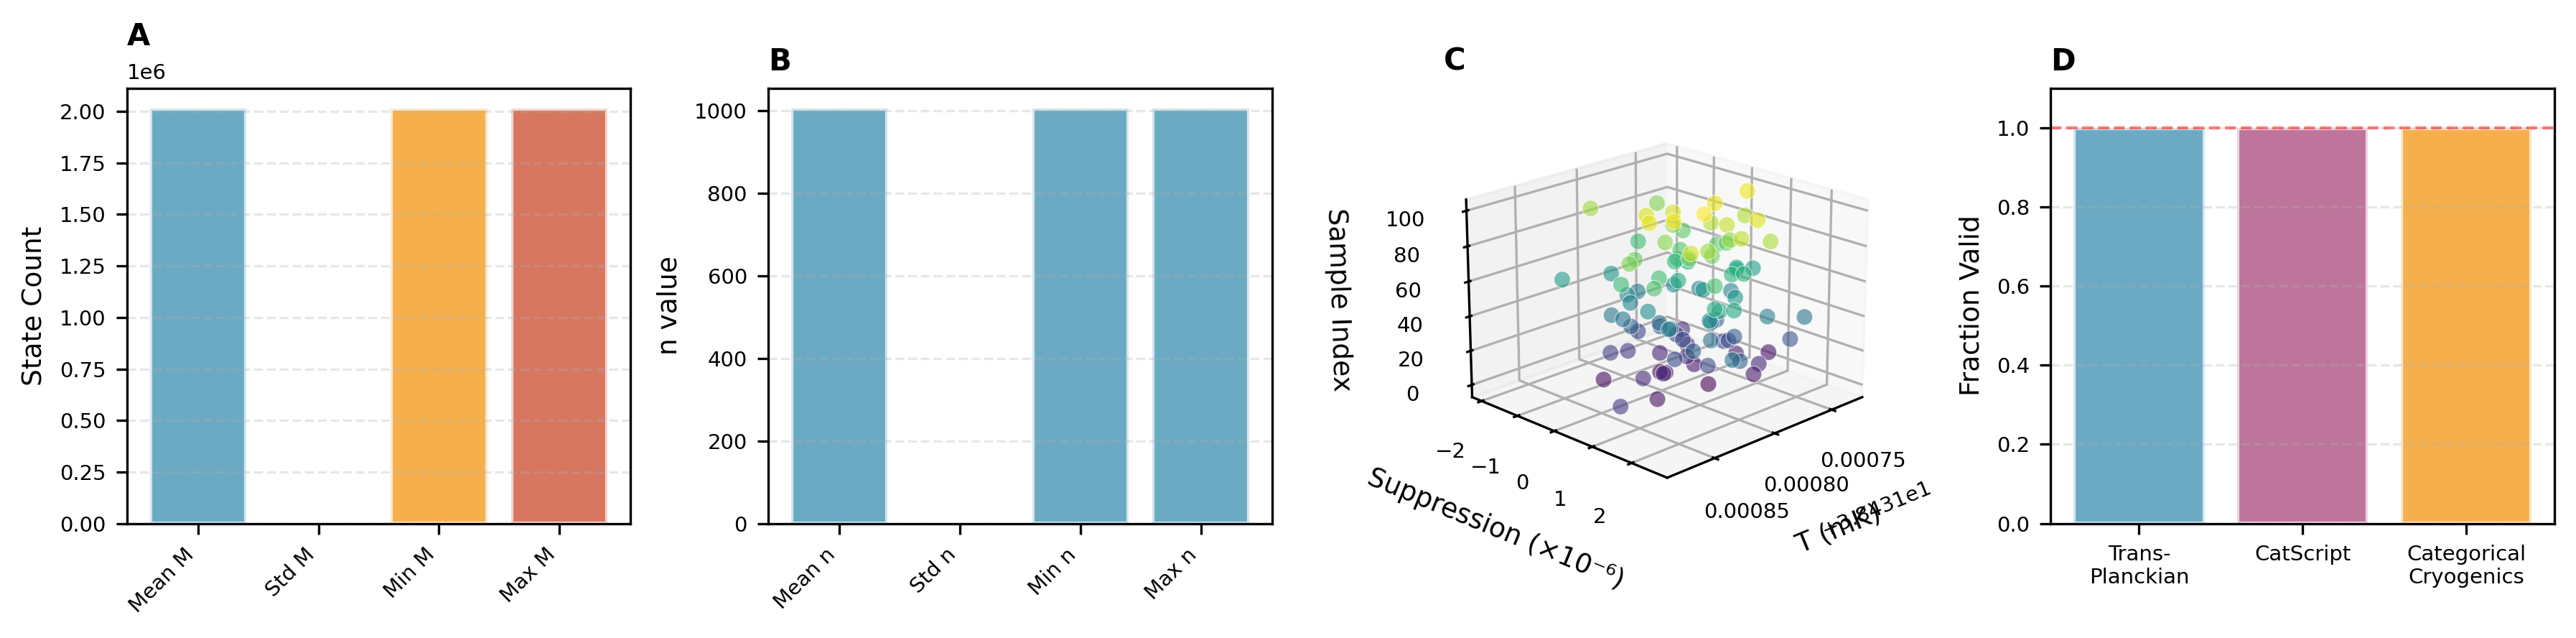
\includegraphics[width=\textwidth]{../../figures/validation_results_20260301_041127_panel_6_statistics.png}
    \caption{\textbf{Supplementary: Statistical Summary
    (synthetic run 041127).}
    Statistical panels as described in Figure~\ref{fig:statistics_canonical}.
    Summary statistics for state count, principal number, categorical
    temperature, and regime distribution across the 8-peak synthetic set.}
    \label{fig:statistics_041127}
\end{figure*}

%-----------------------------------------------------------------------------
% Run 20260301_041230  (Synthetic, intermediate run)
%-----------------------------------------------------------------------------

\begin{figure*}[!htbp]
    \centering
    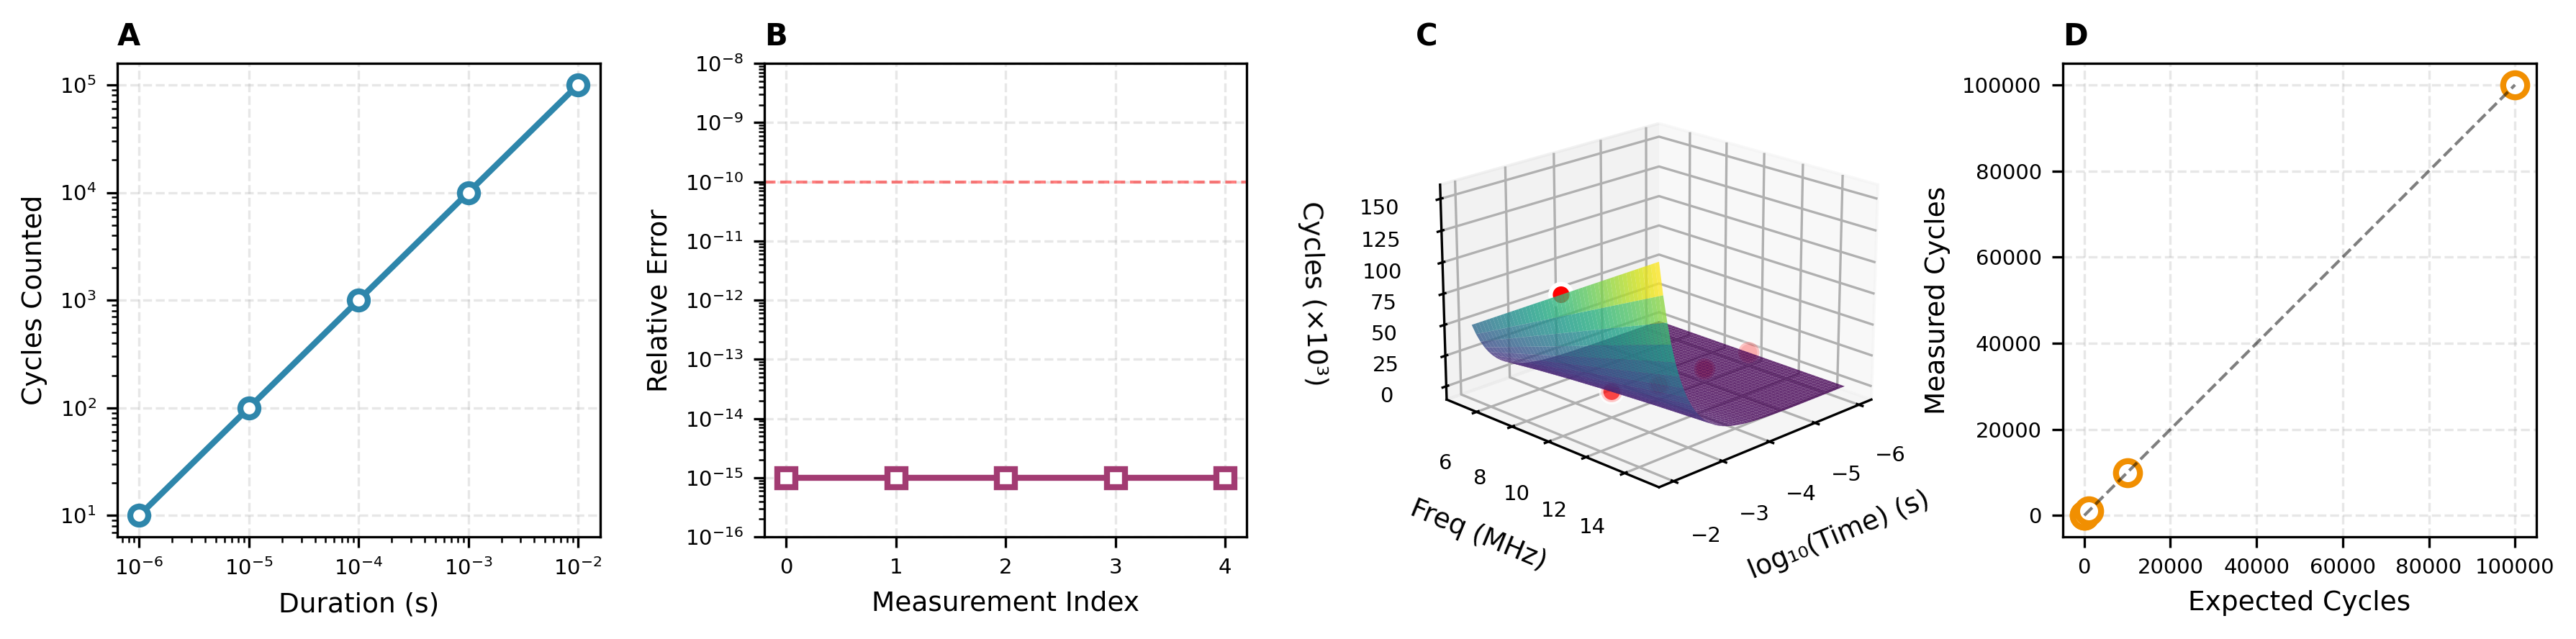
\includegraphics[width=\textwidth]{../../figures/validation_results_20260301_041230_panel_1_oscillator.png}
    \caption{\textbf{Supplementary: Hardware Oscillator Validation
    (synthetic run 041230).}
    Oscillator panels as described in Figure~\ref{fig:oscillator_canonical}.
    Identical results confirm the universality of the counting identity.}
    \label{fig:oscillator_041230}
\end{figure*}

\begin{figure*}[!htbp]
    \centering
    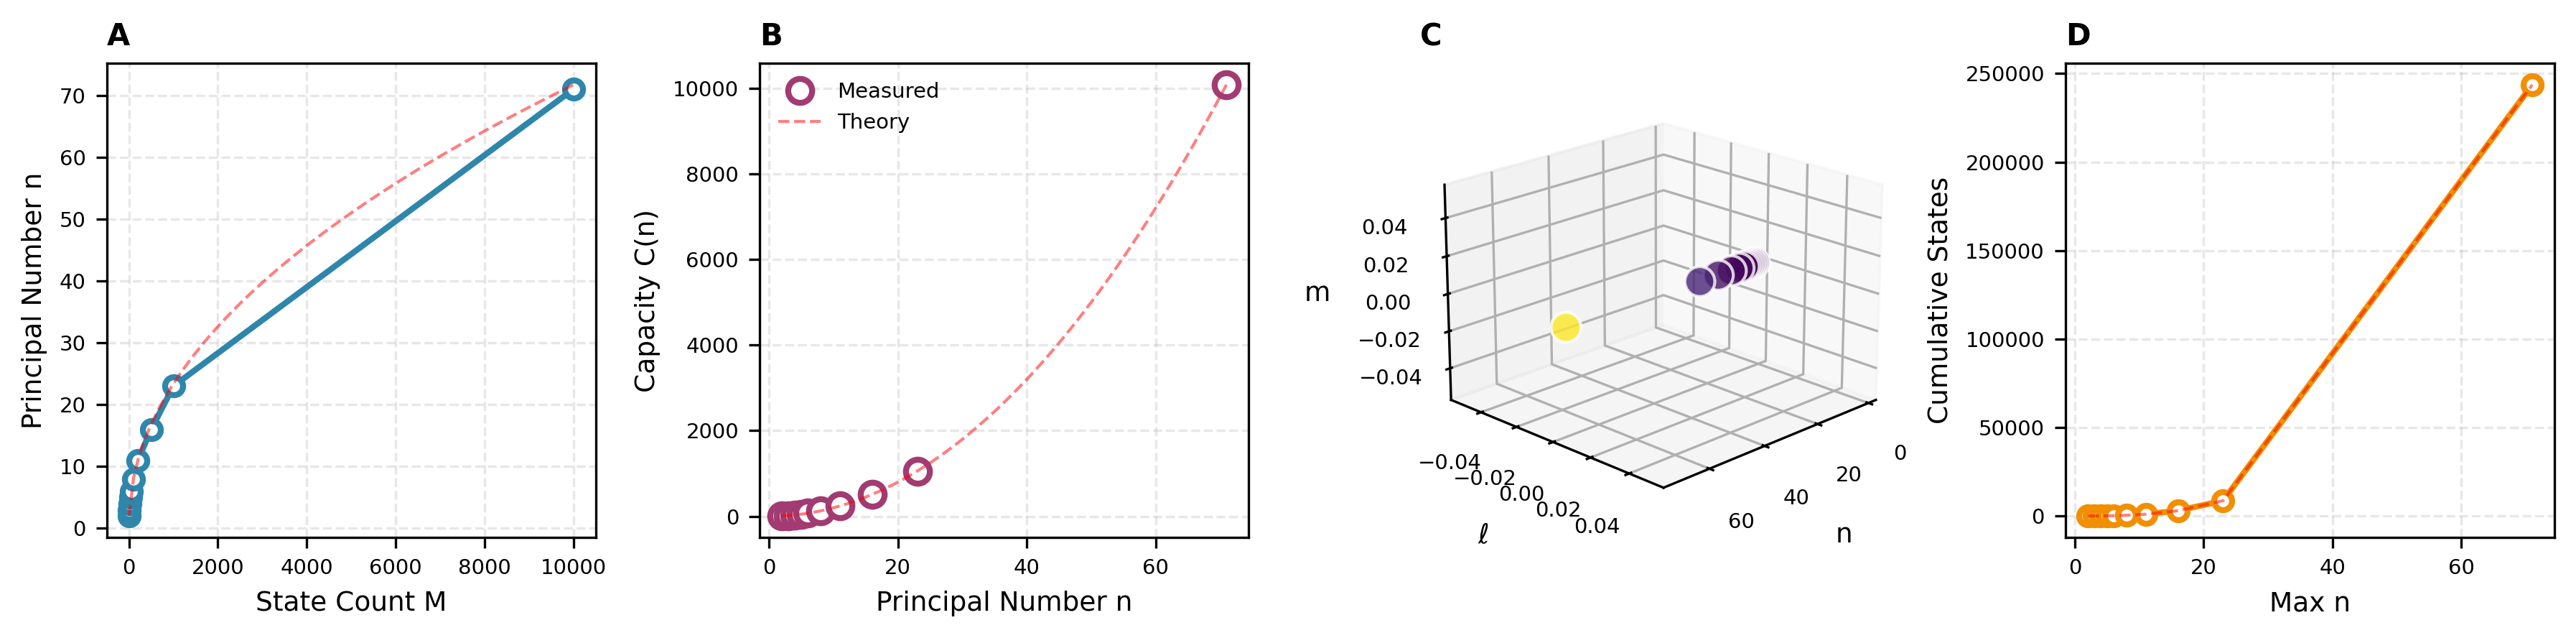
\includegraphics[width=\textwidth]{../../figures/validation_results_20260301_041230_panel_2_partition.png}
    \caption{\textbf{Supplementary: Partition Coordinate Validation
    (synthetic run 041230).}
    Partition panels as described in Figure~\ref{fig:partition_canonical}.
    All 10 test cases satisfy the capacity formula and cumulative count
    identities exactly.}
    \label{fig:partition_041230}
\end{figure*}

\begin{figure*}[!htbp]
    \centering
    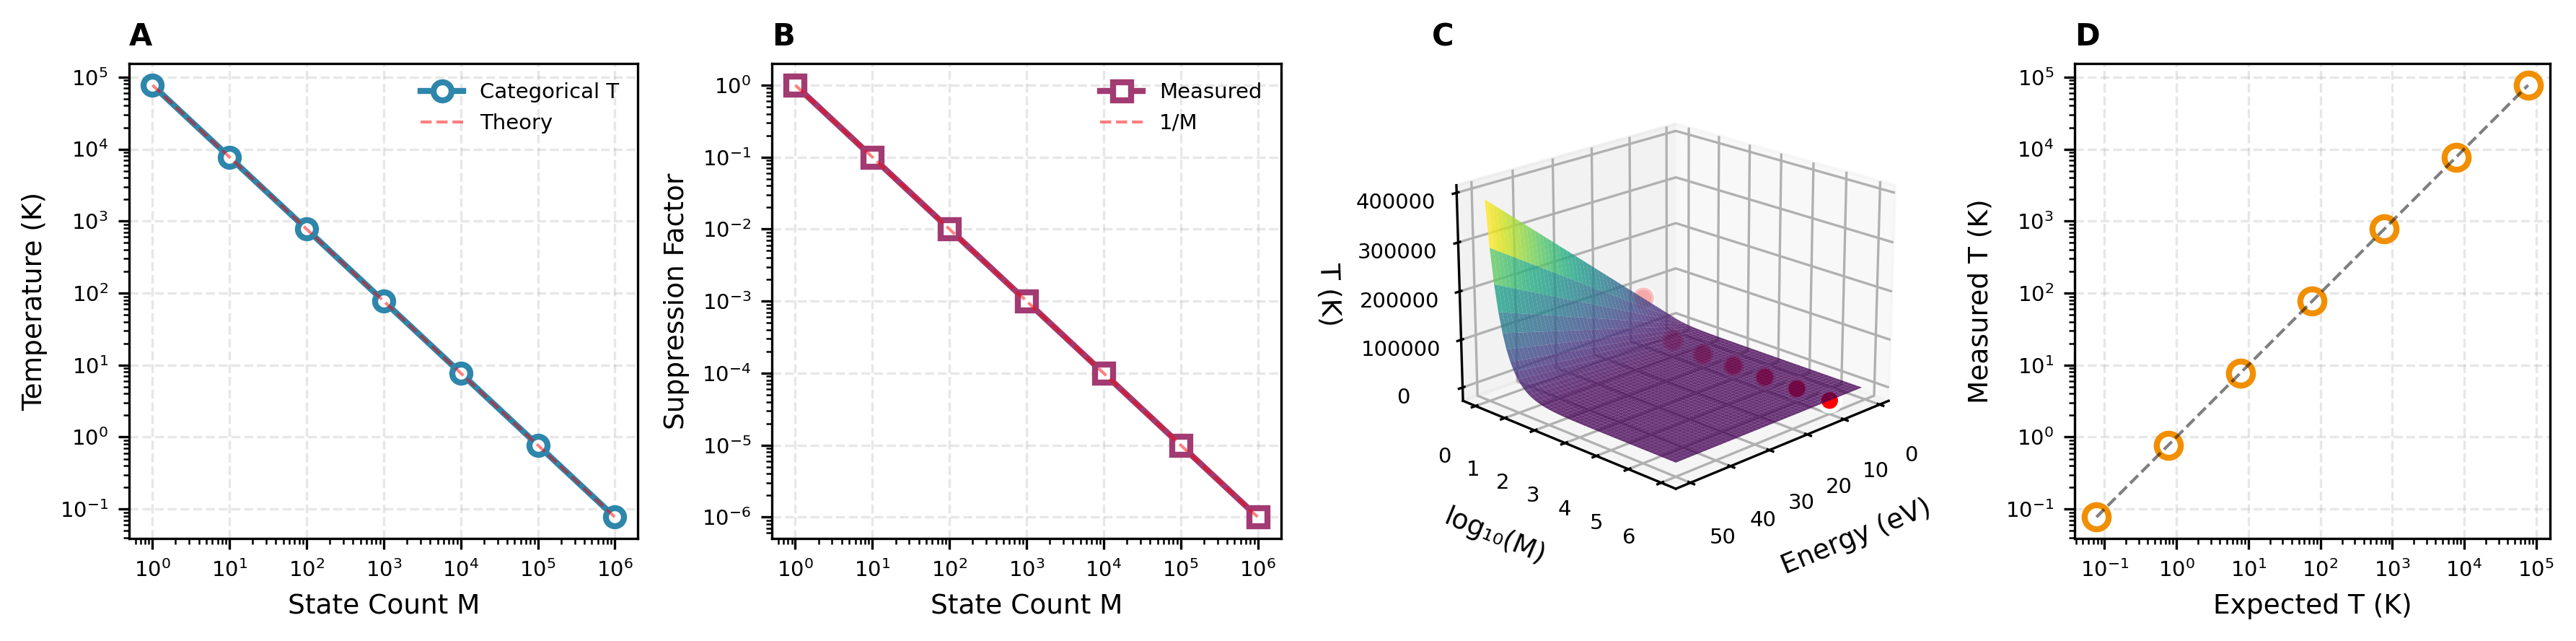
\includegraphics[width=\textwidth]{../../figures/validation_results_20260301_041230_panel_3_temperature.png}
    \caption{\textbf{Supplementary: Categorical Temperature Validation
    (synthetic run 041230).}
    Temperature panels as described in Figure~\ref{fig:temperature_canonical}.
    The $1/M$ suppression law and $T_{\mathrm{cat}} = 2E/(3k_{\mathrm{B}}M)$
    are confirmed at all seven state counts.}
    \label{fig:temperature_041230}
\end{figure*}

\begin{figure*}[!htbp]
    \centering
    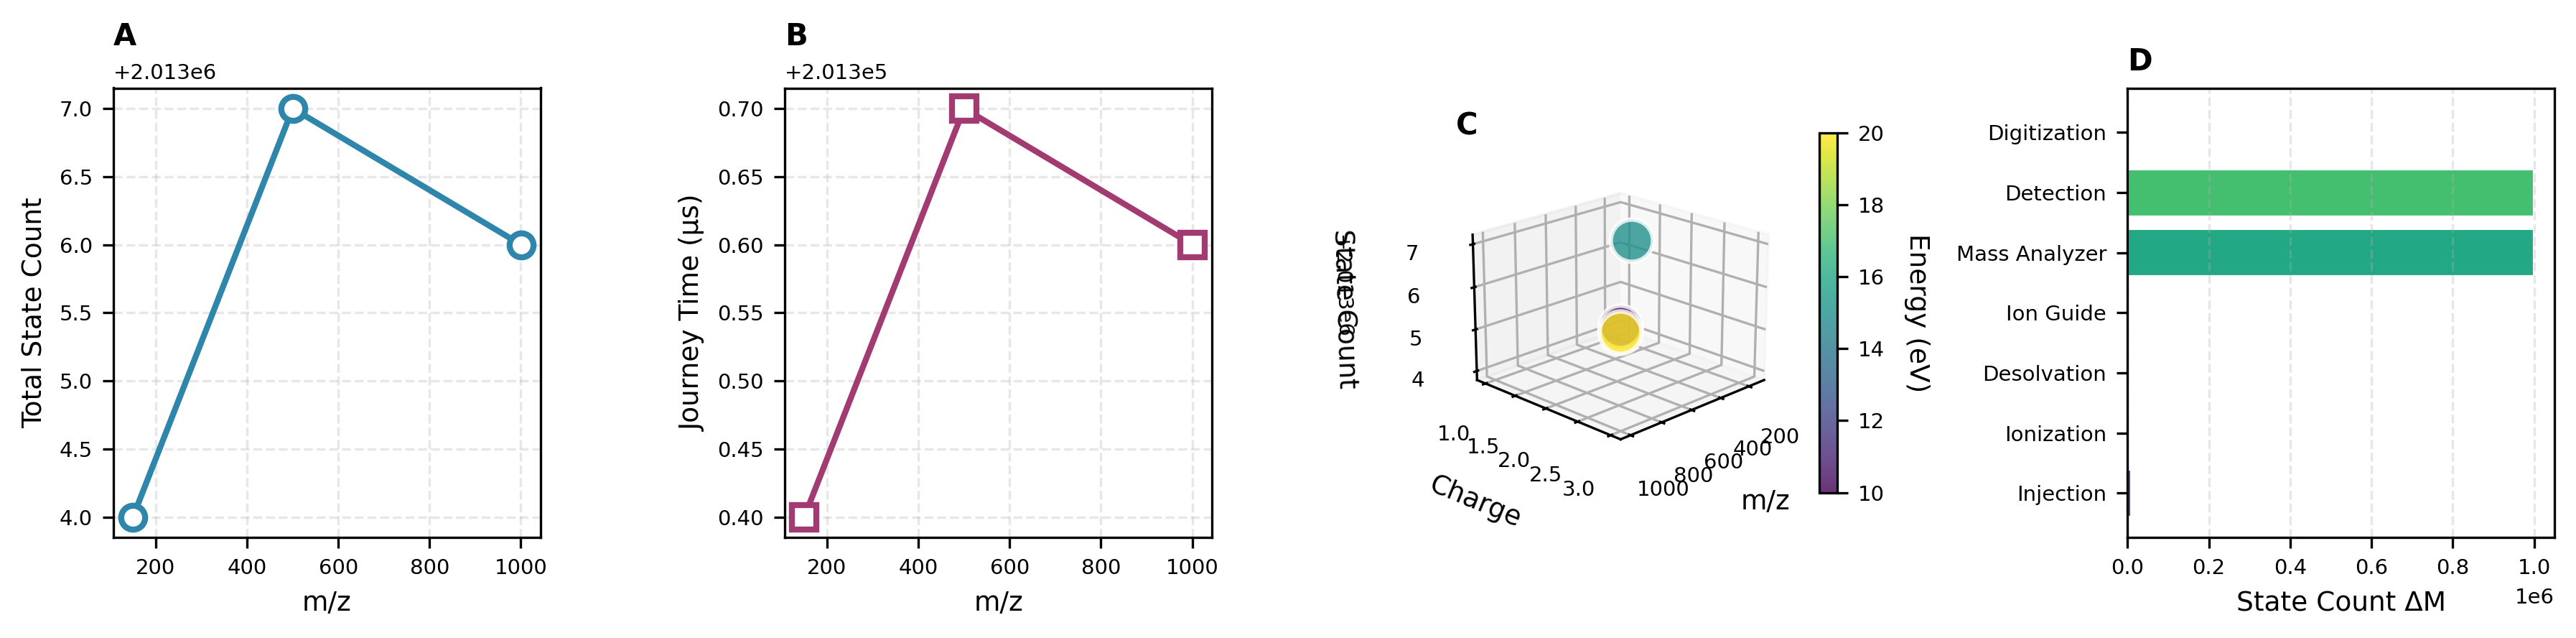
\includegraphics[width=\textwidth]{../../figures/validation_results_20260301_041230_panel_4_trajectory.png}
    \caption{\textbf{Supplementary: Ion Trajectory Validation
    (synthetic run 041230).}
    Trajectory panels as described in Figure~\ref{fig:trajectory_canonical}.}
    \label{fig:trajectory_041230}
\end{figure*}

\begin{figure*}[!htbp]
    \centering
    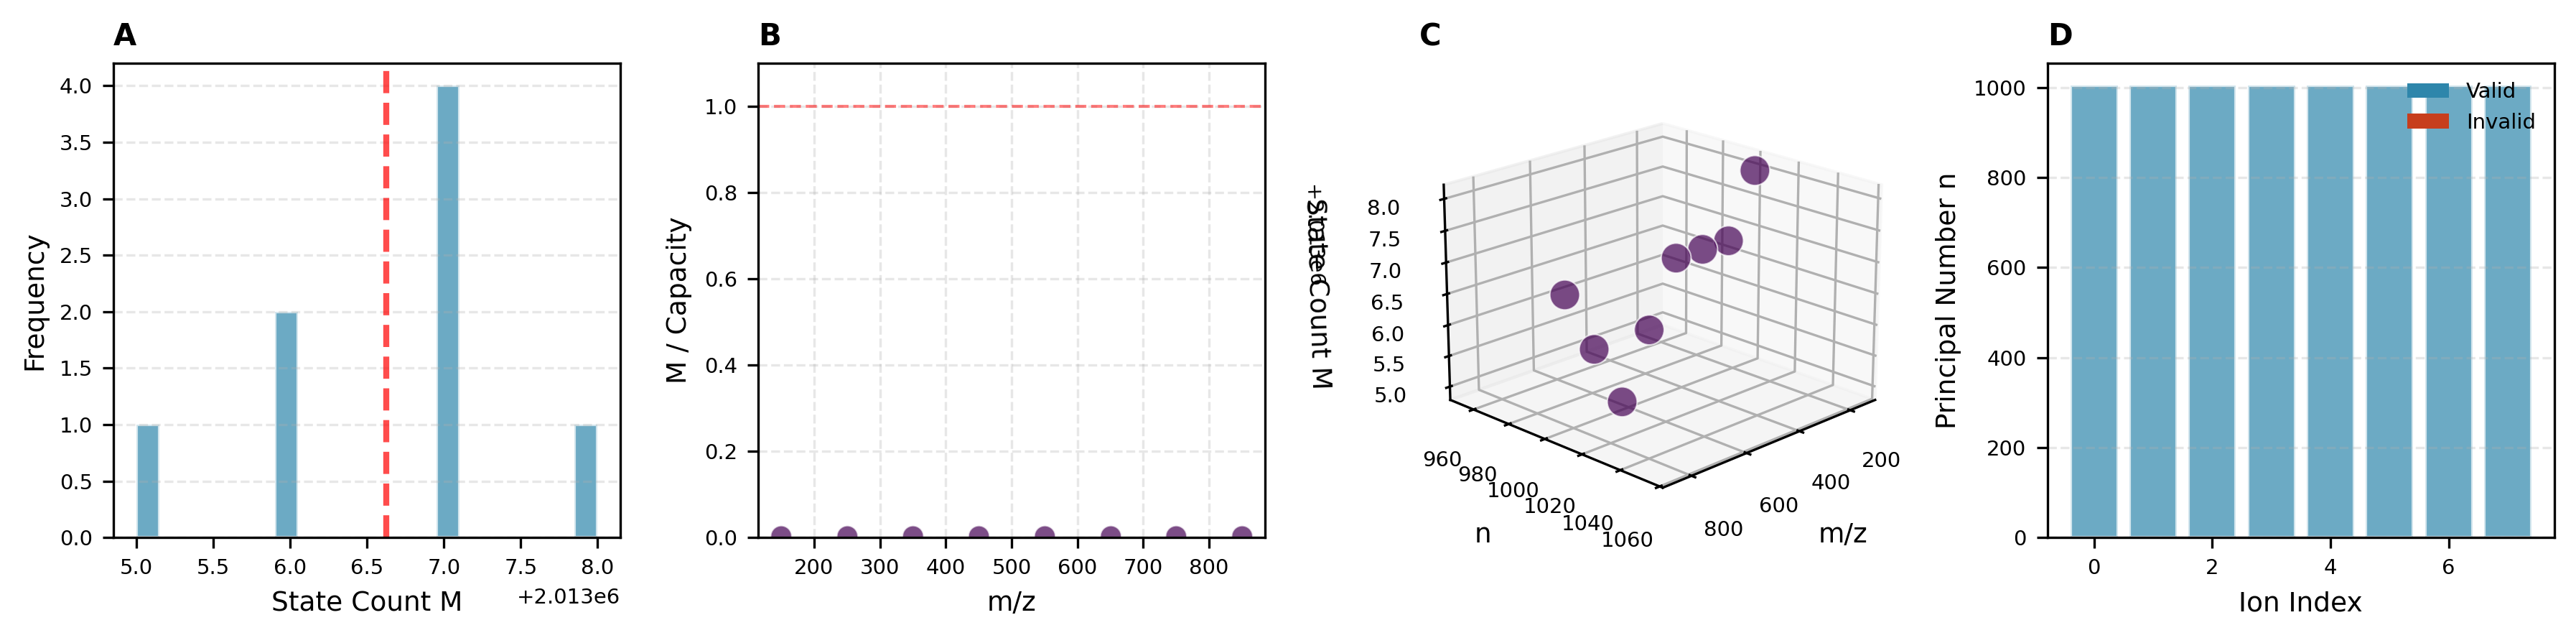
\includegraphics[width=\textwidth]{../../figures/validation_results_20260301_041230_panel_5_pipeline.png}
    \caption{\textbf{Supplementary: Pipeline Validation on Synthetic Data
    (run 041230, 8 synthetic peaks, $m/z \in [150, 850]$~Da).}
    (\textbf{A}) State count histogram.
    (\textbf{B}) Capacity utilisation versus $m/z$.
    (\textbf{C}) Three-dimensional $(m/z, n, M)$ scatter.
    (\textbf{D}) Selection rule compliance; 100\% valid.}
    \label{fig:pipeline_041230}
\end{figure*}

\begin{figure*}[!htbp]
    \centering
    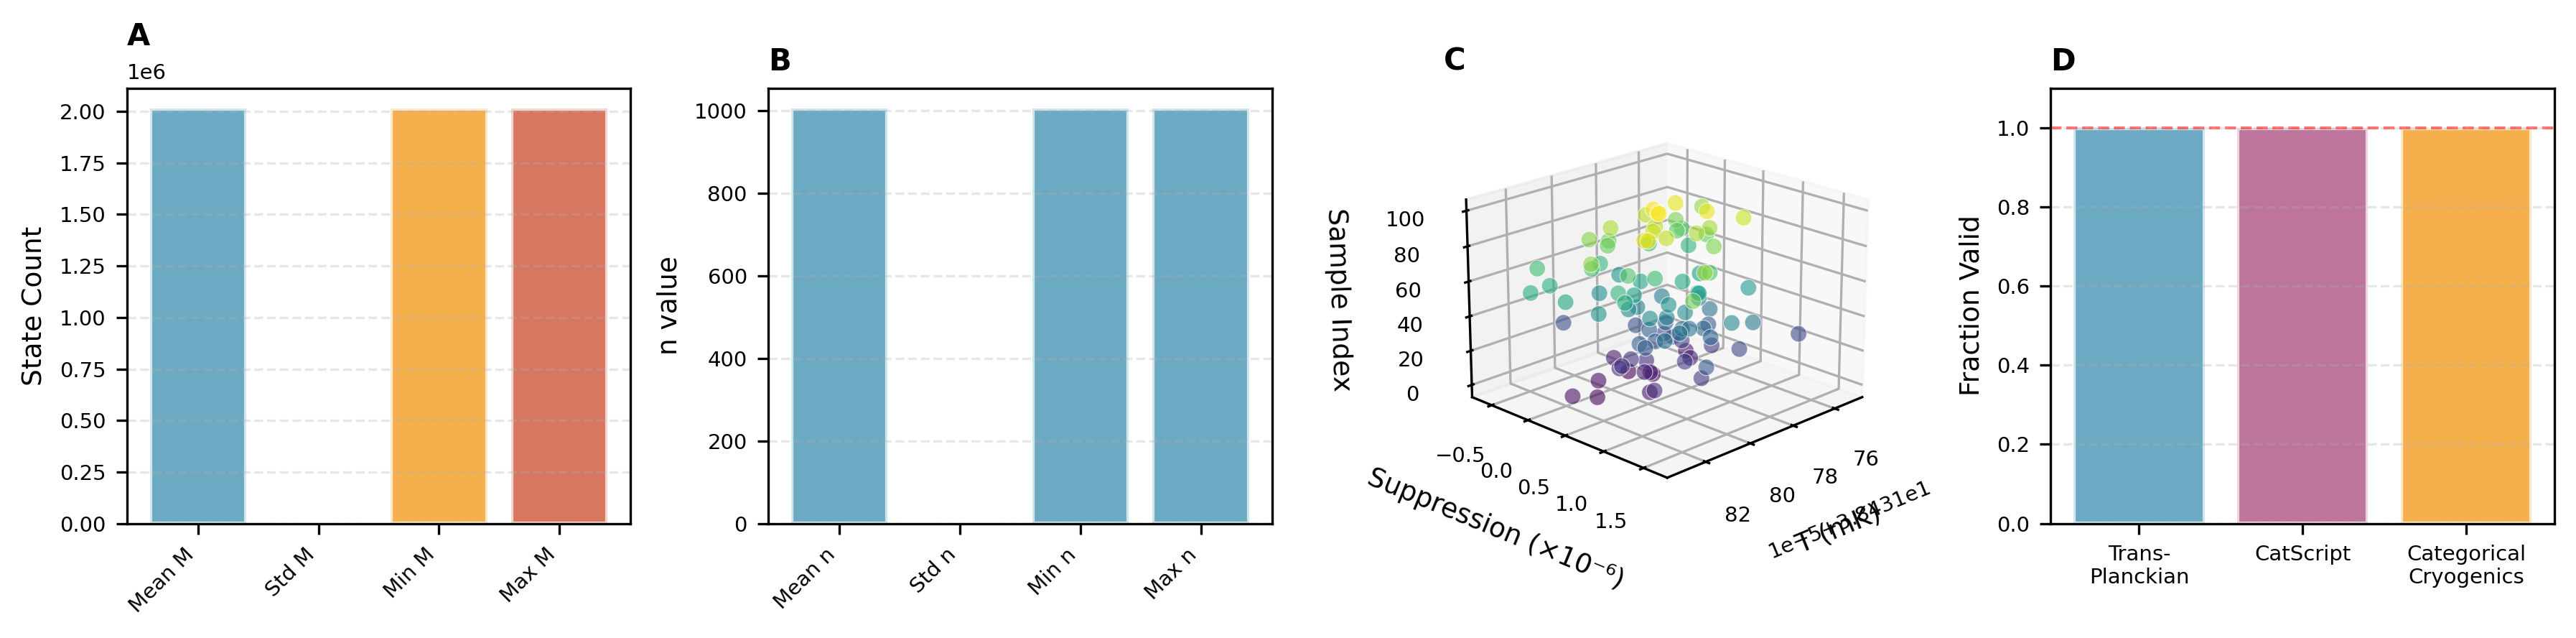
\includegraphics[width=\textwidth]{../../figures/validation_results_20260301_041230_panel_6_statistics.png}
    \caption{\textbf{Supplementary: Statistical Summary
    (synthetic run 041230).}
    Statistical panels as described in Figure~\ref{fig:statistics_canonical}.
    All metrics agree with the canonical run to the precision of the
    synthetic ion parameters.}
    \label{fig:statistics_041230}
\end{figure*}

%=============================================================================
% Usage notes
%
% To include a specific figure in the main manuscript, copy-paste the
% relevant environment from this file. For example, to include the
% canonical oscillator figure:
%
%   \input{captions}  % include entire file
%
% or
%
%   Copy-paste the figure* environment for fig:oscillator_canonical
%   directly into the body of partition-counting.tex.
%
% The \label commands above follow the pattern:
%   fig:{panel}_{run}
% where {panel} is one of: oscillator, partition, temperature, trajectory,
%                           pipeline, statistics
%       {run}   is one of: canonical (041532), 041104, 041127, 041230
%
% For the main manuscript, use the _canonical labels.
% For supplementary materials, use the numbered labels.
%=============================================================================
  % include entire file
%
% or
%
%   Copy-paste the figure* environment for fig:oscillator_canonical
%   directly into the body of partition-counting.tex.
%
% The \label commands above follow the pattern:
%   fig:{panel}_{run}
% where {panel} is one of: oscillator, partition, temperature, trajectory,
%                           pipeline, statistics
%       {run}   is one of: canonical (041532), 041104, 041127, 041230
%
% For the main manuscript, use the _canonical labels.
% For supplementary materials, use the numbered labels.
%=============================================================================
  % include entire file
%
% or
%
%   Copy-paste the figure* environment for fig:oscillator_canonical
%   directly into the body of partition-counting.tex.
%
% The \label commands above follow the pattern:
%   fig:{panel}_{run}
% where {panel} is one of: oscillator, partition, temperature, trajectory,
%                           pipeline, statistics
%       {run}   is one of: canonical (041532), 041104, 041127, 041230
%
% For the main manuscript, use the _canonical labels.
% For supplementary materials, use the numbered labels.
%=============================================================================
  % include entire file
%
% or
%
%   Copy-paste the figure* environment for fig:oscillator_canonical
%   directly into the body of partition-counting.tex.
%
% The \label commands above follow the pattern:
%   fig:{panel}_{run}
% where {panel} is one of: oscillator, partition, temperature, trajectory,
%                           pipeline, statistics
%       {run}   is one of: canonical (041532), 041104, 041127, 041230
%
% For the main manuscript, use the _canonical labels.
% For supplementary materials, use the numbered labels.
%=============================================================================
